\documentclass[openany]{now} % creates
%\pdfoutput=1 % not needed for lualatex
\usepackage{luatexja}
\usepackage[match]{luatexja-fontspec}
\setmainjfont{Hiragino Mincho ProN}
\usepackage{enumerate}
\usepackage{graphicx} \usepackage{bmpsize}
%\usepackage[draft]{graphicx} % uncomment to avoid including images

\graphicspath{{./images/}}
\usepackage{mystyle}
\usepackage{amsmath,amssymb}
\usepackage{notations}

\floatstyle{ruled}
\newfloat{boxfloat}{h}{boxfloat}[chapter]{
\title{Computational Optimal Transport}
\author{%
Gabriel Peyr\'e\\CNRS and DMA, ENS
\and 
Marco Cuturi \\Google and CREST, ENSAE}}

\begin{document}

\maketitle

\begin{verbatim}@article{COTFNT,
year = {2019},
volume = {11},
journal = {Foundations and Trends in Machine Learning},
title = {Computational Optimal Transport},
number = {5-6},
pages = {355--607}
author = {Gabriel Peyr\'e and Marco Cuturi}
}\end{verbatim}

\tableofcontents

\mainmatter


% !TEX root = ../ComputationalOTFnT.tex

\begin{abstract}
最適輸送（OT）理論は、フランスの数学者ガスパール・モンジュ（1746--1818）の言葉を借りて非公式に説明することができる：シャベルを手にした作業員が、建設現場に積まれた大きな砂山を移動させなければならない。作業員の目標は、その砂をすべて使って、指定された形状（例えば、巨大な砂の城）の目標となる砂山を築くことである。当然ながら、作業員は総労力を最小化したいと考え、それは例えばシャベル一杯の砂を運ぶのに要する総距離や総時間として定量化される。
%
OTに関心を持つ数学者たちは、この問題を二つの確率分布——同じ体積を持つ二つの異なる砂山——を比較する問題として定式化する。彼らは、最初の砂山を二番目の砂山へと変形、\emph{輸送}、または再形成するあらゆる可能な方法を考慮し、砂の一粒をある場所から別の場所へ移動させるのにどれだけのコストがかかるかという「局所的な」考慮を用いて、そのような各輸送に「大域的な」コストを関連付ける。数学者たちは、その最小コストの輸送の性質と、その効率的な計算に関心を持っている。
%
その最小コストは分布間の距離を定義するだけでなく、確率分布の空間上に豊かな幾何学的構造をもたらす。その構造は、これらの分布が定義される基礎となる「地上」空間の重要な幾何学的性質を借用するという意味で正準的である。例えば、基礎空間がユークリッド空間である場合、補間、重心、凸性、関数の勾配といった重要な概念は、OT幾何学を備えた分布の空間に自然に拡張される。

%To illustrate this problem, consider the ``mines and factories'' problem: Suppose that the first distribution describes the spatial distribution of a raw resource. Typically, such a raw resource is dug from the earth at several mines. definitionThese resources must be transformed to be of any use, and this is carried out at factories. Ideally, each mine would have next to it a factory able to process its production of raw resources so as to minimize any transportation cost. This is of course not the case in general: factories of varying size and locations are likely to form a distribution with very different caracteristics , whose consumption and locations describe a second distribution. In this example, the cost function might describe

% Despite this relatively abstract description, optimal transport theory answers many basic questions related to the way our economy works, such as in the ``mines and factories'' problem: The first pile of sand is distributed across an entire country, and each grain of sand represents a unit of a useful raw resource; the target pile is peaked where those resources are needed, typically in factories, where they are meant to be processed. In that scenario, one seeks the least costly way to move all these resources, given the knowledge of all costs needed to ship a unit of resource from any storage point to any factory.

OTは多くの場面で、異なる形で（再）発見されてきており、豊かな歴史を持っている。モンジュの先駆的な仕事は工学的問題に動機づけられていたが、1920年代のトルストイ、1940年代のヒッチコック、カントロヴィッチ、クープマンスが物流と経済学におけるその重要性を確立した。ダンツィグは1949年に線形計画法の枠組みの中でこれを数値的に解き、OTに最適化における確固たる基盤を与えた。OTはその後1990年代に解析学者たち、特にブレニエによって再検討され、同時にコンピュータビジョンの分野ではアースムーバー距離の名前で知られるようになった。
%
近年、大規模な問題次元にスケール可能な近似ソルバーの登場により、OTの普及にさらなる革命が起きている。その結果、OTは画像科学（色やテクスチャ処理など）、グラフィックス（形状操作）、機械学習（回帰、分類、生成モデリング）における様々な問題を解決するためにますます活用されるようになっている。

本論文は数値手法に重点を置いてOTをレビューし、新しいアルゴリズムの設計を導くことができるOTの理論的性質を扱う。
%
特に、OTがデータ科学において有用性を見出す助けとなった最近の効率的アルゴリズムの波に焦点を当てる。わずか数年の間に提案されたOTの多くの一般化に重要な位置を与え、それらを統計的推論、カーネル法、情報理論に由来する関連アプローチと結びつける。
%
すべての図は、付属のウェブサイト\footnote{\url{https://optimaltransport.github.io/}}で公開されているコードを用いて再現可能である。このウェブサイトでは書籍プロジェクト「Computational Optimal Transport」を公開している。スライドや計算リソースも掲載されている。
\end{abstract}
%
% !TEX root = ../ComputationalOTFnT.tex

\chapter{序論}
\label{c-intro} % a label for the chapter, to refer to it later



%\begin{rem}[This is a test.]
%\label{rem-test1}
%This is a test.
%\end{rem}
%
%\begin{mdframed}\begin{rem}[This is a test.] This is a test.
%\label{rem-test2}
%\end{rem}
%\end{mdframed}
%
%
%\begin{rem}[This is a test.]
%\begin{mdframed}
%This is a test.
%\label{rem-test2}
%\end{mdframed}
%\end{rem}
%
%Ref to~\ref{rem-test1}.
%
%Ref to~\ref{rem-test2}

最短経路の原理は、人生と科学におけるほとんどの意思決定を導く：ある商品、人、または一つの情報がある地点で利用可能であり、目標地点に送る必要がある場合、可能な限り少ない労力を用いることが望ましい。これは通常、平面上では直線に沿って、より複雑な距離空間では測地線に沿ってアイテムを移動させることで達成される。最適輸送の理論は、一度に一つのアイテムだけを移動させるのではなく、複数のアイテム（またはその連続的な分布）をある配置から別の配置へ同時に移動させる問題に関わる場合に、その直感を一般化する。学校の教師が証言できるように、個人のグループの輸送を計画し、到着時に指定された目標配置に到達するという制約のもとで行うことは、一人の個人に対して行うよりもかなり複雑である。実際、グループや分布の観点で考えることは、\citet{Monge1781}の先駆的な研究で最初に示唆された、より高度な数学的形式主義を必要とする。しかし、その形式主義が一見どれほど複雑に見えようとも、この問題は我々の日常生活と深く具体的なつながりを持っている。輸送は、人であれ商品であれ情報であれ、一つのアイテムだけを移動させることは非常に稀である。物流、生産計画、ネットワークルーティングにおけるすべての主要な経済問題は分布の移動を伴い、その系譜は最適輸送に関するすべての先駆的な文献に現れている。実際、\citet{tolstoi1930methods}、\citet{Hitchcock41}、\citet{Kantorovich42}はすべて実用的な関心に導かれていた。それからわずか数年後、主に1980年代以降になって、数学者たちは\citet{Brenier91}らの研究のおかげで、この理論が凸性、偏微分方程式、統計学との深いつながりを持つ、研究のための肥沃な土壌を提供することを発見した。ミレニアムの変わり目に、コンピュータ科学、画像科学、そしてより一般的にデータ科学の研究者たちは、最適輸送理論が、特徴量の集合や記述子という形で容易に利用可能な分布を、異なるより抽象的な文脈で研究するための非常に強力なツールを提供することを理解した。
%

最適輸送に関するいくつかの参考書が執筆されており、\citeauthor{Villani03}（\citeyear{Villani03,Villani09}）による二つの最近の専門書、\citeauthor{rachev1998mass}（\citeyear{rachev1998mass,rachev1998mass2}）によるもの、そしてより最近では\citet{SantambrogioBook}によるものがある。これらの書籍に例示されるように、この理論におけるより形式的で抽象的な概念は、それ自体で数百ページに値する。最適輸送が応用ツールとして次第に確立されてきた今（例えば経済学において、最近\citet{galichon2016optimal}が提唱したように）、我々はその豊かな文献と計算的な観点のバランスを取ることを試み、データ科学、特に画像科学と機械学習への応用を中心に据えた。この意味で、\citet{kolouri2017optimal}による最近のレビューの動機に従いつつ、より広い範囲をカバーすることを試みる。
%
究極的に、我々の目標はOTの実用的な有効性を支える主要な理論的洞察の概観を提示し、これらの洞察を高速な計算スキームに変換する方法の説明により多くの時間を費やすことである。
%
第\ref{c-continuous}章、第\ref{c-algo-basics}章、第\ref{c-entropic}章、第\ref{c-variational}章、第\ref{c-extensions}章の本体は、確率ベクトルまたは離散ヒストグラムの空間における最適輸送が誘導する幾何学の研究に専ら充てられている。
%
より上級の読者を対象として、同じ章内で薄い灰色のボックスにおいて、離散測度に特化した最適輸送のより一般的な数学的解説も与える。離散測度はその確率の重みによって定義されるが、それらの重みが定義される位置によっても定義される。これらの位置は通常、連続的な距離空間内に取られ、ランダム現象をモデル化するための第二の重要な自由度を与える。
%This corresponds to the case where the support of the considered measures can take arbitrary values in a continuous space, giving a second important degree of freedom, beyond just weights, when comparing probability measures.
%
最後に、第三のそして最も技術的な解説の層は濃い灰色のボックスで示され、離散である必要のない任意の測度を扱い、特に基底測度に関する密度を持つことができる。これは伝統的にOT理論に関するほとんどの古典的教科書のデフォルトの設定であるが、実用的な応用においては一般にそれほど重要な役割を果たさない。
%
第\ref{c-algo-semidiscr}章から第\ref{c-statistical}章は、連続測度と離散測度の相互作用を扱い、したがってより数学的な志向を持つ読者を対象としている。

計算最適輸送の分野は、本稿執筆時点において依然として極めて活発な分野である。したがって、この調査で触れていない多種多様なトピックが存在する。順不同で挙げると、分布的にロバストな最適化\citep{NIPS2015_5745,esfahani2018data,NIPS2018_7534,NIPS2018_8015}（パラメータ推定が、入力データの一定のワッサーシュタイン距離内にある任意のデータ測度の最悪の経験的リスクを最小化することで行われる）、ワッサーシュタイン幾何学におけるランジュバン・モンテカルロサンプリングアルゴリズムの収束\citep{dalalyan2017user,pmlr-v65-dalalyan17a,pmlr-v75-bernton18a}、低次元設定における二乗ユークリッドコストを持つOTをモンジュ・アンペール方程式を用いて解く他の数値手法\citep{froese2011convergent,benamou2014numerical,sulman2011efficient}（注意~\ref{rem:MA}で簡単に言及されるのみ）がある。


%\begin{figure}[h!]
%\centering
%\begin{tabular}{@{}c@{\hspace{5mm}}c@{}}
%
\includegraphics[width=.45\linewidth]{barycenters-1d/bary-eucl}  &
%
\includegraphics[width=.45\linewidth]{barycenters-1d/bary-ot}
%\end{tabular}
%\caption{\label{fig-w-vs-eucl}
%Comparison of Wasserstein vs. Euclidean average. \todo{Blabla}
%}
%\end{figure}


%%%%%%%%%%%%%%%%%%%%%%%%%%%%%%%%%%
\section*{記法}

\begin{itemize}
	\item $\range{n}$：整数の集合$\{1,\dots,n\}$。
	\item $\ones_{n,m}$：$\RR^{n\times m}$のすべての要素が$1$に等しい行列。$\ones_{n}$：全要素が1のベクトル。
	\item $\Identity_n$：サイズ$n\times n$の単位行列。
	\item $u\in\RR^n$に対して、$\diag(u)$は対角成分が$u$でそれ以外が零の$n\times n$行列。
	\item $\simplex_n$：$n$個のビンを持つ確率単体、すなわち$\RR^n_+$における確率ベクトルの集合。
	\item $(\a,\b)$：単体$\simplex_n \times \simplex_m$におけるヒストグラム。
	\item $(\al,\be)$：空間$(\X,\Y)$上に定義された測度。
	\item $\frac{\d\al}{\d\be}$：測度$\al$の$\be$に関する相対密度。
	\item $\density{\al} = \frac{\d\al}{\d x}$：測度$\al$のルベーグ測度に関する密度。
	\item $(\al=\sum_i \a_i \delta_{x_i},\be=\sum_j \b_j \delta_{y_j})$：$x_1,\dots,x_n\in\X$および$y_1,\dots,y_m\in\Y$上に台を持つ離散測度。
	\item $\c(x,y)$：地上コスト、関連するペアワイズコスト行列$\C_{i,j}=(\c(x_i,y_j))_{i,j}$は$\al,\be$の台上で評価される。
	\item $\pi$：$\al$と$\be$の間のカップリング測度、すなわち任意の$A\subset\X$に対して$\pi(A\times \Y)= \al(A)$、かつ任意の部分集合$B\subset \Y$に対して$\pi(\X\times B)= \be(B)$を満たす。離散測度に対して$\pi = \sum_{i,j} \P_{i,j}\delta_{(x_i,y_j)}$。
	\item $\Couplings(\al,\be)$：カップリング測度の集合、離散測度に対して$\CouplingsD(\a,\b)$。
	\item $\Potentials(\c)$：許容双対ポテンシャルの集合；離散測度に対して$\PotentialsD(\C)$。
	\item $\T : \X \rightarrow \Y$：モンジュ写像、典型的には$\T_\sharp \al = \be$を満たす。
	\item $(\al_t)_{t=0}^1$：動的測度、$\al_{t=0}=\al_0$かつ$\al_{t=1}=\al_1$。
	\item $\speed$：ベナムー・ブレニエ定式化における速度；$\Moment=\al \speed$：運動量。
	\item $(\f,\g)$：双対ポテンシャル、離散測度に対して$(\fD,\gD)$は双対変数。
	\item $(\uD,\vD) \eqdef (e^{\fD/\varepsilon},e^{\gD/\varepsilon})$：シンクホーンスケーリング。
	\item $\K \eqdef e^{-\C/\varepsilon}$：シンクホーンのためのギブスカーネル。
	% entropy
	\item $\flow$：$\Wass_1$型問題（ダイバージェンス制約下の最適化）のためのフロー。
	\item $\MKD_\C(\a,\b)$および$\MK_\c(\al,\be)$：コスト$\C$（ヒストグラム）および$\c$（任意の測度）を持つOTに関連する最適化問題の値。
	\item $\WassD_p(\a,\b)$および$\Wass_p(\al,\be)$：地上距離行列$\distD$（ヒストグラム）および距離$\dist$（任意の測度）に関連する$p$-ワッサーシュタイン距離。
	\item $\lambda\in\simplex_S$：$S$個の測度の重心を計算するために使用される重みベクトル。
	\item $\dotp{\cdot}{\cdot}$：通常のユークリッド内積；同じサイズの二つの行列$A$と$B$に対して、$\dotp{A}{B} \eqdef \trace(A^\top B)$はフロベニウス内積。
	\item $\f\oplus \g(x,y) \eqdef f(x)+g(y)$、二つの関数$\f : \X \rightarrow \RR, \g : \Y \rightarrow \RR$に対して、
		$\f \oplus \g : \X\times \Y \rightarrow \RR$を定義する。
	\item $\fD \oplus \gD \eqdef \fD \ones_m^\top + \ones_n \gD^\top \in \RR^{n\times m}$、二つのベクトル$\fD\in\RR^n$、$\gD\in\RR^m$に対して。
	\item $\al \otimes \be$は$\X \times \Y$上の積測度、\ie
		$\int_{\X \times \Y} g(x,y) \d(\al\otimes\be)(x,y) \eqdef \int_{\X \times \Y} g(x,y) \d\al(x) \d\be(y)$。
	\item $\a \otimes \b \eqdef \a \b^\top \in \RR^{n \times m}$。
	\item $\uD \odot \vD = (\uD_i \vD_i) \in \RR^n$、$(\uD, \vD) \in (\RR^n)^2$に対して。
\end{itemize}
% !TEX root = ../ComputationalOTFnT.tex

\chapter{理論的基礎}
\label{c-continuous}

この章では、最適輸送の基礎を説明する。まず確率ベクトル$(\a,\b)$間の最適マッチングとカップリングに関連する概念を導入し、この計算を離散測度$(\al,\be)$間の輸送へと段階的に一般化し、最後に任意の測度に対する一般的な設定を扱う。初読の際には、これらの最後の細部は省略してもよく、読者は確率ベクトル、すなわちヒストグラム間の計算のみに焦点を当てればよい。それが第~\ref{c-algo-basics}章および第~\ref{c-entropic}章で詳述するアルゴリズムを実装するための唯一の前提条件である。より経験豊富な読者は、任意の測度に適用可能な定式化を検討することで問題のより深い理解に到達し、より高度な問題（例えば、点群の位置を移動させる問題や、連続密度から点がサンプリングされる統計的設定など）に適用できるようになるだろう。

%%%%%%%%%%%%%%%%%%%%%%%%%%%%%%%%%%%%%%%%%%%%
\section{ヒストグラムと測度}

確率単体に属する任意の要素$\a \in \simplex_n$に対して、ヒストグラムおよび確率ベクトルという用語を同義に使用する。
\eq{
	\simplex_n \eqdef \enscond{\a \in \RR_+^n}{ \sum_{i=1}^n \a_i = 1 }.
}
本レビューの大部分は、単体上で最適輸送が誘導する幾何学の研究に専ら焦点を当てている。% A more versatile presentation takes advantage of the formalism of discrete measures, which corresponds to handling both the weights contained in a probability vector and the positions associated with the bins of the histogram (the support of the measure). % This formalism can be used implicitly to handle histograms of arbitrary size $n$ and with possibly varying positions. Lastly, the third and most technical layer of exposition deals with arbitrary measures (\ie which need not be discrete, typically continuous with respect to a base measure).


%%%%%%%%%%%%%%
\begin{rem1}{離散測度}
重み$\a$と位置$x_1,\dots,x_n\in\X$を持つ離散測度は次のように表される。
\eql{\label{eq-discr-meas}
	\al = \sum_{i=1}^n \a_i \de_{x_i},
}
ここで$\de_x$は位置$x$におけるディラック測度であり、直感的には位置$x$に無限に集中した単位質量である。このような測度は、さらに$\a\in\simplex_n$であれば確率測度を表し、より一般にベクトル$\a$のすべての要素が非負であれば正測度を表す。質量のない位置が考慮される退化した場合を避けるため、離散測度を考える際には$\a$のすべての要素が正であると仮定する。
\end{rem1}
%%%%%%%%%%%%%%



%%%%%%%%%%%%%%
\begin{rem2}{一般の測度}
最適輸送の便利な特徴は、離散と連続のいずれか、またはその両方の測度を同一の枠組みで扱えることである。そのために、空間$\X$上のラドン測度の集合$\Mm(\X)$を用いる。この集合の厳密な定義には、$\X$が距離（通常$\dist$と記す）を備えていることが必要である。なぜなら、測度には連続関数（$f \in \Cc(\X)$と記す）に対する積分（テスト）を通じてのみアクセスできるからである。

離散測度$\al$に対する$f \in \Cc(\X)$の積分は和として計算される。
\eq{
	\int_\X f(x) \d\al(x) = \sum_{i=1}^n \a_i f(x_i).
}
%
より一般的な測度、例えば$\X=\RR^\dim$（ここで$\dim \in \NN^*$は次元）上の測度は、ルベーグ測度に関する密度$\d\al(x)=\density{\al}(x)\d x$を持つことがある。これはしばしば$\density{\al} = \frac{\d\al}{\d x}$と記され、次を意味する。
\eq{
	\foralls h \in \Cc(\RR^\dim), \quad
	\int_{\RR^\dim} h(x) \d\al(x) =  \int_{\RR^\dim} h(x) \density{\al}(x) \d x.
}
%
任意の測度$\al \in \Mm(\X)$（密度を持つ必要もなく、ディラック測度の和である必要もない）は、任意の連続関数$f \in \Cc(\X)$に対して積分でき$\int_\X f(x) \d\al(x) \in \RR$が得られるという事実によって定義される。$\X$がコンパクトでない場合は、$f$がコンパクト台を持つか、少なくとも無限遠で$0$に収束することも課す必要がある。
%
したがって、測度はある意味で関数より「正則性が低い」が、超関数（滑らかな関数との双対として定義される）よりは正則性が高い。例えば、ディラック測度の導関数は測度ではない。
%
$\Mm_+(\X)$で$\X$上のすべての正測度の集合を表す。確率測度の集合は$\Mm_+^1(\X)$と記され、任意の$\al \in \Mm_+^1(\X)$が正であり、かつ$\al(\X)=\int_\Xx \d\al = 1$であることを意味する。
%
図~\ref{fig-measures}は、本書で考える、ヒストグラム以外のさまざまなクラスの測度の視覚化を提供する。
\end{rem2}
%%%%%%%%%%%%%%


\begin{figure}[h!]
\centering
\begin{tabular}{@{}c@{\hspace{1mm}}c@{\hspace{1mm}}c@{\hspace{1mm}}c@{}}

\includegraphics[width=.24\linewidth]{measures/discrete-1d.pdf}&

\includegraphics[width=.15\linewidth]{measures/discrete-2d}&

\includegraphics[width=.24\linewidth]{measures/density-1d}&

\includegraphics[width=.22\linewidth]{measures/density-2d}\\
離散 $d=1$ & 離散 $d=2$ & 密度 $d=1$ & 密度 $d=2$
\end{tabular}
\caption{\label{fig-measures}
離散分布$\al = \sum_{i=1}^n \a_i \de_{x_i}$（赤は経験的一様分布$\a_i=1/n$に対応し、青は任意の分布に対応）および密度$\d\al(x)=\density{\al}(x)\d x$（紫）の模式図。1次元および2次元の場合を示す。1次元の離散分布はステムプロット（長さは$\a_i$に等しい）で表示され、2次元では点群を用いて表示される（この場合、半径は$\a_i$に等しいか、より視覚的に正確な表現として面積が$\a_i$に等しい）。
}
\end{figure}





%%%%%%%%%%%%%%%%%%%%%%%%%%%%%%%%%%%%%%%%%%%%
\section{割当問題とモンジュ問題}

コスト行列$(\C_{i,j})_{i \in \range{n}, j \in \range{m}}$が与えられ、$n=m$と仮定すると、最適割当問題は$n$個の要素の置換の集合$\Perm(n)$における全単射$\si$を求める問題であり、次を解く。
\eql{\label{eq-optimal-assignment}
	\umin{\si \in \Perm(n)} \frac{1}{n}\sum_{i=1}^n \C_{i,\si(i)}.
}
素朴には、集合$\Perm(n)$のすべての置換を用いて上記のコスト関数を評価できる。しかし、その集合のサイズは$n!$であり、小さな$n$でさえ巨大である。例えば、$n$がわずか70でもその集合は$10^{100}$を超える要素を持つことを考えよ~\citep{Dantzig1983}。したがって、この問題は置換の集合上でコスト関数を最適化する効率的なアルゴリズムが存在する場合にのみ解くことができ、それが\S\ref{s-auction}の主題である。

\begin{rem}[一意性] 最適割当問題は複数の最適解を持つ場合があることに注意せよ。例えば、$n=m=2$であり、行列$\C$が辺の長さ$1$の2次元正方形の4つの頂点間のペアワイズ距離行列であるとする（図~\ref{fig-non-unique-matching}の左のプロットに示す）。この場合、2つの割当のみが存在し、両方とも最適である。
\end{rem}


\begin{figure}[h!]
\centering

\includegraphics[width=.8\linewidth]{non-unique-optimal-matching/non-unique-optimal-matching}
\caption{\label{fig-non-unique-matching}
左：測度$\alpha$の青い点と測度$\beta$の赤い点はペアワイズに等距離である。したがって、マッチング$\sigma=(1,2)$（実線）と$\sigma=(2,1)$（点線）の両方が最適である。右：モンジュ写像は青い測度$\alpha$を赤い測度$\beta$に対応させることができる。重み$\alpha_i$は各位置のディスクの面積に比例して表示されている。ここでの写像は$T(x_1)=T(x_2)=y_2$、$T(x_3)=y_3$であり、$4\leq i\leq 7$に対して$T(x_i)=y_1$である。
}
\end{figure}


%%%%%%%%%
\begin{rem1}{離散測度間のモンジュ問題}\label{rem-monge1}
離散測度
\eql{\label{eq-pair-discr}
	\al = \sum_{i=1}^n \a_i \de_{x_i}
	\qandq
	\be = \sum_{j=1}^m \b_j \de_{y_j},
}
に対して、\citeauthor{Monge1781}の問題~\citeyearpar{Monge1781}は、各点$x_i$を単一の点$y_j$に対応させ、$\al$の質量を$\be$の質量に押し出す写像を求める。すなわち、写像$T:\{x_1,\dots, x_n\}\rightarrow \{y_1,\dots,y_m\}$は次を満たさなければならない。
\eql{\label{eq-monge-constr}
	\foralls j \in \range{m}, \quad
	\b_j = \sum_{ i : \T(x_i) = y_j } \a_i ,
}
これをコンパクトな形で$\T_\sharp \al = \be$と書く。$\b$のすべての要素が正であるため、この写像は必然的に全射である。
%
この写像は、点$(x,y) \in \X \times \Y$に対して定義されるコスト関数$\c(x,y)$によってパラメータ化される輸送コストを最小化しなければならない。
\eql{\label{eq-monge-discr}
	\umin{\T} \enscond{ \sum_{i} \c(x_i,\T(x_i))  }{ \T_\sharp \al = \be } .
}
このような離散点間の写像は、すべての$x$および$y$が異なると仮定すれば、添字$\si : \range{n} \rightarrow \range{m}$を用いて$j=\si(i)$のように符号化でき、質量保存は次のように書かれる。
\eq{
	\sum_{i \in \si^{-1}(j)} \a_i = \b_j,
}
ここで逆$\si^{-1}(j)$は$j$の原像集合として理解する。$n=m$かつすべての重みが一様、すなわち$\a_i=\b_j=1/n$である特殊な場合には、質量保存制約は$\T$が全単射であることを意味し、$\T(x_i)=y_{\si(i)}$となり、モンジュ問題は最適マッチング問題~\eqref{eq-optimal-assignment}と等価になる。ここでコスト行列は
\eq{
	\C_{i,j} \eqdef \c(x_i,y_j).
}
$n\ne m$の場合、最適性は別として、モンジュ写像はある離散測度から別の離散測度へ存在しないこともあることに注意せよ。これは重みベクトルが両立しない場合に起こり、目標測度がソース測度より多くの点を持つ場合、すなわち$n<m$の場合に常にそうなる。例えば、図~\ref{fig-non-unique-matching}の右のプロットは$\al$から$\be$への（最適な）モンジュ写像を示しているが、$\be$から$\al$へのモンジュ写像は存在しない。
\end{rem1}
%%%%%%%%%


%%%%%%%
\begin{rem2}{押し出し作用素}\label{rem-push-f}
連続写像$\T : \X \rightarrow \Y$に対して、対応する押し出し作用素$\T_\sharp : \Mm(\X) \rightarrow \Mm(\Y)$を定義する。
%
離散測度~\eqref{eq-discr-meas}に対して、押し出し操作は単に測度の台にあるすべての点の位置を移動させることからなる。
\eq{
	\T_{\sharp} \al \eqdef \sum_i \a_i \de_{\T(x_i)}.
}
より一般的な測度に対して、例えば密度を持つ測度に対しては、押し出しの概念は確率測度の空間的な変更（または輸送）を記述する上で基本的な役割を果たす。厳密な定義は以下のとおりである。

\begin{defn}[押し出し]\label{defn-pushfwd}
$\T : \X \rightarrow \Y$に対して、ある$\al \in \Mm(\X)$の押し出し測度$\be = \T_\sharp \al \in \Mm(\Y)$は次を満たす。
\eql{\label{eq-push-fwd}
	\foralls h \in \Cc(\Y), \quad \int_\Y h(y) \d \be(y) = \int_\X h(\T(x)) \d\al(x).
	% = \int_X h(T(x)) \density{\al}(x) \d x %%%% y=T(x)   dy=|T'(x)| dx
	% = \int_Y h(y) \density{\al}(T^{-1}(y)) 1/|T'(x)| \d y
	% = \int_Y h(y) \density{\be}(y) \d y
	%  \density{\al}(T^{-1}(y)) 1/|T'(x)| = \density{\be}(y)
}
同値な表現として、任意の可測集合$B \subset \Y$に対して、次が成り立つ。
\eql{\label{eq-equiv-pushfwd}
	\be(B) = \al( \enscond{x \in \X}{\T(x) \in B} ) = \al( T^{-1}(B) ).
}
$\T_\sharp$は正値性と全質量を保存するので、$\al \in \Mm_+^1(\X)$ならば$\T_\sharp \al \in \Mm_+^1(\Y)$となることに注意せよ。
\end{defn}

直感的には、可測写像$T: \X\rightarrow \Y$は単一の点をある可測空間から別の可測空間へ移動させる関数として解釈できる。$T_\sharp$は$T$の拡張であり、$\X$上の確率測度全体を$\Y$上の新しい確率測度へ移動させることができる。作用素$T_\sharp$は、測度$\al$の各要素的質量を写像$T$を適用して$\X$上から$\Y$上の要素的質量へと\emph{押し出す}。押し出し作用素$\T_\sharp : \Mm_+^1(\X) \rightarrow \Mm_+^1(\Y)$は、2つの測度$\al_1,\al_2$に対して$T_\sharp(\al_1+\al_2)=T_\sharp\al_1+ T_\sharp\al_2$という意味で\emph{線形}であることに注意せよ。
\end{rem2}
%%%%%%%

%%%%%%%
\begin{rem2}{多変量密度に対する押し出し}
$\RR^\dim$上の密度$(\density{\al},\density{\be})$を持つ測度に対して（$\T$が滑らかで全単射であると仮定して）、公式~\eqref{eq-push-fwd}における変数変換を明示的に行うと、押し出しが積分公式における変数変換として密度に対して線形に作用することが示される。実際、次が成り立つ。
\eql{\label{eq-pfwd-density}
	\density{\al}(x) = |\det(\T'(x))|  \density{\be}(\T(x)),
}
ここで$\T'(x) \in \RR^{\dim \times \dim}$は$T$のヤコビ行列（$T$の各座標の勾配を取って形成される行列）である。
これは次を意味する。
\eq{
	|\det(\T'(x))| = \frac{ \density{\al}(x) }{ \density{\be}(\T(x)) }.
}
\end{rem2}
%%%%%%%


%%%%%%%
\begin{rem2}{任意の測度間のモンジュ問題}\label{rem-monge2}
モンジュ問題~\eqref{eq-monge-discr}は、2つの任意の確率測度$(\al,\be)$が2つの空間$(\X,\Y)$上に台を持ち、写像$\T : \X \rightarrow \Y$を通じて結ばれる場合に拡張でき、次を最小化する。
\eql{\label{eq-monge-continuous}
	\umin{\T} \enscond{ \int_{\X} \c(x,\T(x)) \d \al(x)  }{  \T_\sharp \al = \be }.
}
制約$\T_\sharp \al = \be$は、$\T$が$\al$の質量を$\be$へ押し出すことを意味し、注意~\ref{rem-push-f}で定義された押し出し作用素を用いている。
\end{rem2}
%%%%%%%


%%%%%%%
\begin{rem2}{押し出しと引き戻し}
測度の押し出し$\T_\sharp$は、関数の引き戻し$\T^\sharp : \Cc(\Y) \rightarrow \Cc(\X)$と混同してはならない。後者は関数間の「ワーピング」に対応し、$g \in \Cc(\Y)$に$\T^\sharp g = g \circ \T$を対応させる線形写像として定義される。押し出しと引き戻しは実際には互いに随伴であり、次の意味においてそうである。
\eq{
	\foralls (\al,g) \in \Mm(\X) \times \Cc(\Y), \quad
	\int_\Y g \d( \T_\sharp\al ) = \int_\X (\T^\sharp g) \d\al.
}
$(\al,\be)$が固定された測度（例えば$\RR^\dim$上のルベーグ測度）に関する密度$(\density{\al},\density{\be})$を持つ場合でも、$\T_\sharp \al$は~\eqref{eq-pfwd-density}におけるヤコビアンの存在により$\T^\sharp \density{\be}$を密度として持つわけではないことに注意せよ。
%
これが、最適輸送を画像レジストレーションに使用する際に注意が必要な理由である。なぜなら、最適輸送は画像ワーピング法としては機能しないからである。
%
図~\ref{fig-push-pull}はこれらの押し出しと引き戻し作用素の区別を示している。
\end{rem2}
%%%%%%%


\begin{figure}[h!]
\centering
\begin{tabular}{@{}c@{\hspace{5mm}}c@{}}

\includegraphics[width=.3\linewidth]{push-pull/push-forward}&

\includegraphics[width=.3\linewidth]{push-pull/pull-back}\\
測度の押し出し & 関数の引き戻し
\end{tabular}
\caption{\label{fig-push-pull}
押し出し作用素$\T_\sharp$（任意の測度を入力として取ることができる）と引き戻し作用素$\T^\sharp$（関数、特に密度に作用する）の比較。
}
\end{figure}



%%%%%%%%%%%%%%
\begin{rem2}{測度と確率変数}\label{rem-meas-random}
	ラドン測度は確率変数の分布を表すものとしても見ることができる。$\X$上の確率変数$X$は実際にはある抽象的な（しばしば不特定の）確率空間$(\Om,\PP)$からの写像$X : \Om \rightarrow \X$であり、その分布$\al$は$\PP(X \in A) = \al(A)=\int_A \d\al(x)$を満たすラドン測度$\al \in \Mm_+^1(\X)$である。
	%
	同値に、これは$\PP$の$X$による押し出し$\al=X_\sharp\PP$である。
	%
	$\T : \X \rightarrow \Y$に対して別の押し出し$\be = \T_\sharp\al$を~\eqref{eq-push-fwd}に従って適用することは、別の確率変数$Y=\T(X) : \om \in \Om \rightarrow \T(X(\om)) \in Y$を定義することと等価であり、$\be$は$Y$の分布となる。
	%
	$Y$からのランダムサンプル$y$の抽出は、$X$から抽出した$x$に対して単に$y=\T(x)$を計算することで達成される。
\end{rem2}
%%%%%%%%%%%%%%


%%%%%%%%%%%%%%%%%%%%%%%%%%%%%%%%%%%%%%%%%%%%
\section{カントロヴィッチ緩和}\label{sec-kantorovich-relaxation}

%%%%%
%\paragraph{Limitations of the Monge Problem}

割当問題、および注意~\ref{rem-monge1}で提示されたモンジュ問題におけるその一般化は、実際の問題に見られるような離散測度を研究するために常に適切とは限らない。実際、割当問題は置換問題として定式化されているため、\emph{同じ}サイズの\emph{一様な}ヒストグラムの比較にのみ使用できる。非一様な重みを持つ離散測度への直接的な一般化はモンジュの押し出し写像の形式を用いて行うことができるが、質量保存制約~\eqref{eq-monge-constr}を満たす実行可能解が存在しない場合にはその定式化も退化し得る（注意~\ref{rem-monge1}の末尾を参照）。さらに、割当問題~\eqref{eq-monge-discr}は組合せ的であり、モンジュ問題~\eqref{eq-monge-continuous}の実行可能集合は、質量保存制約を満たすすべての押し出し測度からなる集合として連続的にパラメータ化されているにもかかわらず、\emph{非凸}である。したがって、いずれも元の定式化のまま取り組むと解くことが困難である。

%%%%%%
% \paragraph{Kantorovich's relaxation} Redundant
\citet{Kantorovich42}の鍵となるアイデアは、輸送の決定論的な性質、すなわちソース点$x_i$が別の点または位置$y_{\sigma_i}$あるいは$T(x_i)$にのみ割り当てられるという事実を緩和することである。カントロヴィッチは代わりに、任意の点$x_i$の質量が複数の位置に分配される可能性を提案する。カントロヴィッチは質量輸送が\emph{決定論的}であるべきという考えから離れ、代わりに\emph{確率論的}な輸送を考え、現在一般に\emph{質量分割}として知られるもの、すなわちソースから複数のターゲットへの分割を可能にする。この柔軟性は、置換$\sigma$や写像$T$の代わりに、カップリング行列$\P  \in \RR_+^{n \times m}$を用いて符号化される。ここで$\P_{i,j}$はビン$i$からビン$j$へ、あるいは離散測度~\eqref{eq-pair-discr}の形式では$x_i$から$y_j$へ流れる質量の量を表す。許容カップリングはモンジュ写像よりもはるかに単純な特徴付けを持つ。
\eql{\label{eq-discr-couplings}
	\CouplingsD(\a,\b) \eqdef \enscond{ \P \in \RR_+^{n \times m} }{
		\P \ones_m = \a \qandq
		\transp{\P} \ones_n = \b
	},
}
ここで次の行列-ベクトル記法を用いた。
\eq{
	\P \ones_m = \left(\sum_j \P_{i,j}\right)_i \in \RR^n
	\qandq
	\transp{\P} \ones_n = \left(\sum_i \P_{i,j}\right)_j \in \RR^m.
}
行列の集合$\CouplingsD(\a,\b)$は有界であり$n+m$個の等式制約で定義されるため、凸多面体（有限個の行列の凸包）である~\citep[\S8.1]{brualdi2006combinatorial}。

%
さらに、モンジュの定式化（図~\ref{fig-non-unique-matching}の右のプロットに示すように）が本質的に非対称であるのに対し、カントロヴィッチの緩和された定式化は常に対称的である。すなわち、カップリング$\P$が$\CouplingsD(\a,\b)$に属するのは$\transp{\P}$が$\CouplingsD(\b,\a)$に属する場合であり、かつその場合に限る。カントロヴィッチの最適輸送問題は次のように読まれる。
\eql{\label{eq-mk-discr}
	\MKD_{\C}(\a,\b) \eqdef
	\umin{\P \in \CouplingsD(\a,\b)}
		\dotp{\C}{\P} \eqdef \sum_{i,j} \C_{i,j} \P_{i,j}.
}
これは線形計画問題であり（第~\ref{c-algo-basics}章を参照）、そのような計画問題の場合に通常そうであるように、その最適解は必ずしも一意ではない。

\begin{rem}[鉱山と工場]\label{rem-kantorovich-primal} カントロヴィッチ問題は、以下の資源配分問題において非常に自然な例示を見出す（\citet{Hitchcock41}も参照）。ある事業者が$n$個の倉庫と$m$個の工場を運営しているとする。各倉庫には工場が適切に稼働するために必要な貴重な原材料が含まれている。より正確には、各倉庫は整数$i$でインデックス付けされ、$\a_i$単位の原材料を含む。これらの原材料はすべて工場に移動させなければならず、工場$j$が適切に機能するためには所定の量$\b_j$が必要である。倉庫$i$から工場$j$へ資源を移送するために、事業者は1単位の資源を位置$i$から位置$j$に移動させるのに$\C_{i,j}$を請求する運送会社を利用できる。運送会社は輸送の独占権を持ち、経済のすべての主体に同一の線形価格体系を適用するものとする。すなわち、$i$から$j$へ$a$単位の資源を輸送するコストは$a\times \C_{i,j}$に等しい。

上記の問題に直面して、事業者は式~\eqref{eq-mk-discr}で記述される線形計画問題を解き、各ペア$i,j$に対して倉庫$i$から工場$j$へ輸送すべき物品の量$\P_{i,j}$を定量化する輸送計画$\P^\star$を得ることを選択する。事業者はその計画を実行するために、運送会社に合計$\dotp{\P^\star}{\C}$を支払う。
\end{rem}

%%%%%%%
\paragraph{カップリングとしての置換行列}

置換$\si\in\Perm(n)$に対して、対応する置換行列を$\P_{\si}$と書く。
	\eql{\label{eq-perm-matrices}
		\foralls (i,j) \in \range{n}^2, \quad
		(\P_{\si})_{i,j} = \choice{
			1/n \qifq j=\si_i, \\
			0 \quad\text{otherwise.}
		}
	}
この場合、次を確認できる。
\eq{\dotp{\C}{\P_{\si}}=\frac{1}{n}\sum_{i=1}^n \C_{i,\si_i},}
これは割当問題~\eqref{eq-optimal-assignment}が、カップリング$\P$を正確に置換行列に制限したカントロヴィッチ問題~\eqref{eq-mk-discr}として書き直せることを示している。
\eq{\umin{\si \in \Perm(n)} \frac{1}{n}\sum_{i=1}^n \C_{i,\si(i)} = \umin{\si \in \Perm(n)} \dotp{\C}{\P_{\si}}.}
次に、置換行列の集合が\citeauthor{birkhoff}多面体$\CouplingsD(\ones_n/n,\ones_n/n)$に真に含まれることが容易に確認できる。実際、任意の置換$\si$に対して$\P_{\si}\ones=\ones_n$かつ$\transp{\P_{\si}}\ones=\ones_n$が成り立つ一方、$\ones_n\transp{\ones_n}/n^2$は有効なカップリングであるが置換行列ではない。したがって、$\dotp{\C}{\P}$の最小値は、置換行列のみを考える場合よりもすべての輸送計画を考える場合のほうが必然的に小さい。
$$ \MKD_{\C}(\ones_n/n,\ones_n/n) \leq \umin{\si \in \Perm(n)} \dotp{\C}{\P_{\si}}.$$

次の命題は、これらの問題が実際には同じ最適値をもたらすこと、すなわち2つの一様測度$\a=\b=\ones_n/n$間のカントロヴィッチ問題~\eqref{eq-mk-discr}を最小化する置換行列が常に見つかることを示す。したがって、カントロヴィッチ緩和は割当問題において\emph{タイト}である。%Note however that some computational algorithm, which are combinatorial in nature, are dedicated to the case of uniform histograms with the same number of points (see Chapter~\ref{c-algo-basics}).
%
図~\ref{fig-matching-kantorovitch}の左側には、この特殊ケースに対応する最適マッチングの2次元の例を示す。
%

\begin{prop}[マッチングに対するカントロヴィッチ]\label{prop-matching-kanto}
	$m=n$かつ$\a=\b=\ones_n/n$ならば、問題~\eqref{eq-mk-discr}の最適解$\P_{\si^\star}$が存在し、それは問題~\eqref{eq-optimal-assignment}の最適置換$\si^\star \in \Perm(n)$に対応する置換行列である。
\end{prop}

\begin{proof}
	\citeauthor{birkhoff}の定理~\citeyearpar{birkhoff}は、$\CouplingsD(\ones_n/n,\ones_n/n)$の端点の集合が置換行列の集合に等しいことを述べている。線形計画の基本定理~\citep[Theorem 2.7]{bertsimas1997introduction}は、空でない多面体上の線形目的関数の最小値は、有限であれば、多面体の端点で達成されることを述べている。
\end{proof}

\begin{figure}[h!]
\centering
\begin{tabular}{@{}c@{\hspace{5mm}}c@{}}

\includegraphics[width=.4\linewidth]{matching-kantorovitch/matching}&

\includegraphics[width=.4\linewidth]{matching-kantorovitch/weighted}
\end{tabular}
\caption{\label{fig-matching-kantorovitch}
%
最適マッチングと一般的なカップリングの比較。$x_i$と$y_j$の間の黒い線分は、表示された最適カップリング$\P_{i,j}$の~\eqref{eq-mk-discr}を解く非ゼロ要素を示す。
%
左：最適マッチング。命題~\ref{prop-matching-kanto}の設定（同じ点数$n=m$の経験測度）に対応。
%
右：これら2つの重み付き点群はマッチングできない。代わりに、カントロヴィッチカップリングを用いて2つの任意の離散測度を対応させることができる。
}
\end{figure}


%%%%%%%
\begin{rem1}{離散測度間のカントロヴィッチ問題}
形式~\eqref{eq-pair-discr}の離散測度$\al,\be$に対して、$\al,\be$の台の点間のすべてのペアワイズコストを行列$\C$に格納する。すなわち$\C_{i,j} \eqdef \c(x_i,y_j)$として、次を定義する。
\eql{\label{eq-kanto-discr}
	\MK_\c(\al,\be) \eqdef \MKD_{\C}(\a,\b).
}
したがって、離散測度間の最適輸送のカントロヴィッチ定式化は、コスト行列$\C$が$\al$と$\be$の台に依存することを除いて、それらに対応する確率重みベクトル$\a,\b$間の問題と同じである。ただし、記法$\MK_\c(\al,\be)$はある状況で有用である。なぜなら、確率重みと台の点の\emph{両方}への依存性を明示するからであり、後者はコスト関数$\c$を通じてのみ考慮される。
\end{rem1}
%%%%%%%


\begin{figure}[h!]
\centering
\begin{tabular}{@{}c@{\hspace{5mm}}c@{\hspace{5mm}}c@{}}

\includegraphics[width=.3\linewidth]{settings/discrete}&

\includegraphics[width=.3\linewidth]{settings/semi-discrete}&

\includegraphics[width=.3\linewidth]{settings/continuous}\\
離散 & 半離散 & 連続
\end{tabular}
\caption{\label{fig-settings}
カントロヴィッチ最適輸送の3つの主要なシナリオで遭遇する入力測度$(\al,\be)$とカップリング$\Couplings(\al,\be)$の模式図。第~\ref{c-algo-semidiscr}章は半離散の設定に特化している。
}
\end{figure}



%%%%%%%
\begin{rem1}{最適割当とカップリングの応用}
最適輸送計画それ自体（カップリング$\P$またはモンジュ写像$\T$が存在する場合のいずれかとして）は、データサイエンス、特に画像処理において多くの応用を見出している。例えば、コントラスト均等化~\citep{delon2004midway}やテクスチャ合成~\citet{gutierrez2017optimal}に使用されてきた。
%
画像科学への最適輸送の応用の重要な部分は、画像マッチング~\citep{zhu2007image,wang2013linear,museyko2009application,li2013novel}、画像融合~\citep{courty2016optimal}、医用画像処理~\citep{wang2011optimal}、形状レジストレーション~\citep{makihara2010earth,lai2014multi,su2015optimal}、および画像透かし~\citep{mathon2014optimal}に関するものである。天体物理学では、最適輸送は初期宇宙の再構成に使用されてきた~\citep{FrischNaturee}。
%
最適輸送は音楽の採譜~\citep{flamary2016optimal}にも使用されており、経済学ではマッチングデータの解釈に多数の応用がある~\citep{galichon2016optimal}。
%
最後に、最適輸送技術を用いて（またはそれに着想を得て）計算された輸送写像は、サンプリング~\citep{reich2013nonparametric,oliver2014minimization}やベイズ推論~\citep{kim2013efficient,el2012bayesian}を行う上でも有用であることを記しておく。
\end{rem1}
%%%%%%%


%%%%%%%
\begin{rem2}{任意の測度間のカントロヴィッチ問題} $\MK_\c$の定義~\eqref{eq-kanto-discr}は、積空間上の同時分布であるカップリング$\pi \in \Mm_+^1(\X \times \Y)$を考えることにより任意の測度に拡張される。離散の場合は、この積測度を$\pi = \sum_{i,j} \P_{i,j} \de_{(x_i,y_j)}$の形に課す特殊な状況である。一般の場合、質量保存制約~\eqref{eq-discr-couplings}は同時確率分布に対する周辺制約として書き直されるべきである。
\eql{\label{eq-coupling-generic}
	\Couplings(\al,\be) \eqdef
	\enscond{
		\pi \in \Mm_+^1(\X \times \Y)
	}{
		P_{\X\sharp} \pi = \al
		\qandq
		P_{\Y\sharp} \pi = \be
	}.
}
ここで$P_{\X\sharp}$と$P_{\Y\sharp}$は射影$P_\X(x,y)=x$と$P_\Y(x,y)=y$の押し出し（定義~\ref{defn-pushfwd}を参照）である。
%
図~\ref{fig-settings}は、異なるクラスの問題（離散測度と密度）に対してこれらのカップリング制約がどのように変換されるかを示している。
%
\eqref{eq-equiv-pushfwd}を用いると、これらの周辺制約は集合$A \subset \X$および$B \subset \Y$に対して$\pi(A \times \Y)=\al(A)$かつ$\pi(\X \times B)=\be(B)$を課すことと等価である。
%
カントロヴィッチ問題~\eqref{eq-mk-discr}は次のように一般化される。
\eql{\label{eq-mk-generic}
	\MK_\c(\al,\be) \eqdef
	\umin{\pi \in \Couplings(\al,\be)}
		\int_{\X \times \Y} \c(x,y) \d\pi(x,y).
}
これは測度の空間上の無限次元線形計画問題である。$(\X,\Y)$がコンパクト空間で$c$が連続であれば、常に解が存在することを容易に示せる。実際、$\Couplings(\al,\be)$は測度の弱位相に対してコンパクトであり（注意~\ref{dfn-weak-conv}を参照）、$\pi \mapsto \int c \d\pi$はこの位相に対する連続関数であり、制約集合は空でない（例えば$\al \otimes \be \in \Couplings(\al,\be)$）。
%
図~\ref{fig-couplings}は~\eqref{eq-mk-generic}を解く離散および連続の最適カップリングの例を示す。
%
図~\ref{fig-couplings-simple}は離散および連続の周辺分布を含む、最適な1次元カップリングの他の例を示す。
%
\todoK{Explain that proof of existence of minimizers (\ie the inf is a min) follows from classical reasoning in variational calculus, especially if the spaces $(\X,\Y)$ are compact (or the support of the input measure) and the cost $\c$ is continuous. Indeed, the topology to use is the weak topology of measure (Definition~\ref{dfn-weak-conv}) and then the function is continuous on a compact. }
\end{rem2}
%%%%%%%

\begin{figure}[h!]
\centering
\begin{tabular}{@{}c@{\hspace{10mm}}c@{}}

\includegraphics[width=.3\linewidth]{couplings/couplings-continuous}&

\includegraphics[width=.3\linewidth]{couplings/couplings-discr}
\end{tabular}
\caption{\label{fig-couplings}
左：密度を持つ2つの1次元測度間の~\eqref{eq-coupling-generic}を解く「連続」カップリング$\pi$。カップリングはモンジュ写像のグラフ$(x,\T(x))$に沿って局在化している（黒で表示）。
%
右：形式~\eqref{eq-pair-discr}の2つの離散測度間の~\eqref{eq-mk-discr}を解く「離散」カップリング$\T$。正のエントリ$\T_{i,j}$は位置$(i,j)$に$\T_{i,j}$に比例する半径の黒いディスクとして表示されている。
}
\end{figure}


\begin{figure}[h!]
\centering
\begin{tabular}{@{}c@{}c@{}c@{}c@{}}

\includegraphics[width=.24\linewidth]{couplings/couplings-1}&

\includegraphics[width=.24\linewidth]{couplings/couplings-2}&

\includegraphics[width=.24\linewidth]{couplings/couplings-3}&

\includegraphics[width=.24\linewidth]{couplings/couplings-4}
\end{tabular}
\caption{\label{fig-couplings-simple}
1次元分布間の最適カップリングの4つの簡単な例。上に写像として（矢印）、下にカップリングとして表現されている。\citet{Levy2017review}に着想を得た。
}
\end{figure}



%%%%%%%%%%%%%%
\begin{rem2}{確率論的解釈}
カントロヴィッチの問題は、注意~\ref{rem-meas-random}に従い、確率変数のプリズムを通じて再解釈できる。実際、問題~\eqref{eq-mk-generic}は次と等価である。
\eql{\label{eq-ot-proba-interpretation}
	\MK_\c(\al,\be) = \umin{(X,Y)} \enscond{ \EE_{(X,Y)}(c(X,Y)) }{ X \sim \al, Y \sim \be },
}
ここで$(X,Y)$は$\X \times \Y$上の確率変数の組であり、$X \sim \al$（あるいは$Y \sim \be$）は$X$（あるいは$Y$）の法則が測度として$\al$（あるいは$\be$）でなければならないことを意味する。組$(X,Y)$の法則は、積空間$\X \times \Y$上の$\pi \in \Couplings(\al,\be)$である。
\end{rem2}
%%%%%%%%%%%%%%



%%%%%%%%%%%%%%%%%%%%%%%%%%%%%%%%%%%%%%%%%%%%
\section{最適輸送の距離的性質}

最適輸送の重要な特徴は、コスト行列が適切な性質を満たす限り、ヒストグラムおよび確率測度間の距離を定義することである。実際、最適輸送は点間の基底距離をヒストグラムまたは測度間の距離に持ち上げる正準的な方法として理解できる。

まず、\citet{RubTomGui00}によって最初に導入された用語を用いて、「基底計量」行列$\C$が固定され、ビン間の置換コストを表し、比較したい複数のヒストグラムにわたって共有される場合を考える。次の命題は、最適輸送がこれらのビン上に台を持つヒストグラム間の有効な距離を提供することを述べている。

\begin{prop}\label{prop-metric-histo}
$n=m$とし、ある$p \geq 1$に対して$\C=\distD^p=(\distD_{i,j}^p)_{i,j} \in \RR^{n \times n}$とする。ここで$\distD \in \RR_+^{n \times n}$は$\range{n}$上の距離であり、すなわち
\begin{enumerate}[label=(\roman*)]
	\item $\distD \in \RR_+^{n \times n}$は対称である。
	\item $\distD_{i,j}=0$であるのは$i=j$の場合に限る。
	\item $\foralls (i,j,k) \in \range{n}^3, \distD_{i,k} \leq \distD_{i,j}+\distD_{j,k}$。
\end{enumerate}
このとき
\eql{\label{eq-wass-p-disc}
	\WassD_p(\a,\b) \eqdef \MKD_{\distD^p}(\a,\b)^{1/p}
}
（$\WassD_p$は$\distD$に依存することに注意）は$\Si_n$上の$p$-ワッサーシュタイン距離を定義する。すなわち$\WassD_p$は対称であり、正であり、$\WassD_p(\a,\b)=0$であるのは$\a = \b$の場合に限り、三角不等式
\eq{
	\foralls \a,\b,\VectMode{c} \in \Si_n, \quad \WassD_p(\a,\VectMode{c}) \leq \WassD_p(\a,\b) + \WassD_p(\b,\VectMode{c}).
}
を満たす。
\end{prop}

\begin{proof}
距離の対称性と正定値性は容易に証明できる。$\C = \distD^p$は対角成分が零であるから、$\WassD_p(\a,\a)=0$であり、対応する最適輸送行列は$\P^\star=\diag(\a)$である。$\distD^p$のすべての非対角要素の正値性により、$\a\ne \b$のとき$\WassD_p(\a,\b)>0$である（この場合、許容カップリングは必然的に対角の外側に非ゼロ要素を持つため）。$\distD^p$の対称性により、$\WassD_p(\a,\b)$自体が対称関数である。


任意の測度に対するワッサーシュタイン距離の三角不等式を証明するために、\citet[Theorem 7.3]{Villani03}は貼り合わせ補題を用い、所定の構造を持つカップリングの存在を強調する。
% Closed forms for such couplings exist in the discrete case which we can readily use.
離散設定では、この貼り合わせカップリングの明示的な構成は簡単である。
%
$\a,\b,\VectMode{c} \in\simplex_n$とする。$\P$と$\Q$をそれぞれ$\a$と$\b$間、および$\b$と$\VectMode{c}$間の輸送問題の2つの最適解とする。
%
$\b$のゼロ座標から生じ得る問題を回避するため、$\tilde\b_j \eqdef \b_j$（$\b_j>0$の場合）、$\tilde{\b}_j\eqdef 1$（それ以外の場合）となるベクトル$\tilde{\b}$を定義し、次を書く。
\eq{
	\SS \eqdef \P \diag(1/\tilde{\b}) \Q \in \RR_+^{n \times n},
}
そして$\SS \in \CouplingsD(\a,\VectMode{c})$であることに注意する。なぜなら
\eq{
	\SS \ones_n  = \P \diag(1/\tilde{\b}) \Q \ones_n = \P (\b / \tilde{\b}) = \P \ones_{\Supp(\b)} = \a,
}
ここで$\ones_{\Supp(\b)}$は$\b_j>0$であるインデックス$j$の位置に1を持ちそれ以外はゼロであるサイズ$n$のベクトルを表し、$\b_j=0$であるような$j$に対しては必然的に$\P_{i,j} = 0$であるから$\P \ones_{\Supp(\b)} = \P \ones = \a$であるという事実を用いている。同様に$\transp{\SS} \ones_n = \VectMode{c}$が確認できる。三角不等式は次から従う。
\begin{align*}
\WassD_p(\a,\VectMode{c})&=\left(\min_{\P\in U(\a,\VectMode{c})}\dotp{\P}{\distD^p}\right)^{1/p} \leq \dotp{\SS}{\distD^p}^{1/p}\\
&= \left(\sum_{ik} \distD^p_{ik}\sum_{j} \frac{\P_{ij}\Q_{jk}}{\tilde{\b}_j}\right)^{1/p} \leq \left(\sum_{ijk} \left(\distD_{ij}+\distD_{jk}\right)^p \frac{\P_{ij}\Q_{jk}}{\tilde{\b}_j}\right)^{1/p} \\
& \leq \left(\sum_{ijk} \distD^p_{ij} \frac{\P_{ij}\Q_{jk}}{\tilde{\b}_j}\right)^{1/p} + \left(\sum_{ijk}\distD^p_{jk} \frac{\P_{ij}\Q_{jk}}{\tilde{\b}_j}\right)^{1/p}.
\end{align*}
第一の不等式は$\SS$の準最適性による。第二は$\distD$の要素に対する三角不等式であり、第三はミンコフスキーの不等式から来る。したがって次を得る。
\begin{align*}
\WassD_p(\a,\VectMode{c})& \leq \left(\sum_{ij} \distD^p_{ij}\P_{ij} \sum_k \frac{\Q_{jk}}{\tilde{\b}_j}\right)^{1/p} + \left(\sum_{jk} \distD^p_{jk} \Q_{jk} \sum_i \frac{\P_{ij}}{\tilde{\b}_j}\right)^{1/p}\\
&= \left(\sum_{ij} \distD^p_{ij}\P_{ij}\right)^{1/p} + \left(\sum_{jk} \distD^p_{jk} \Q_{jk}\right)^{1/p}\\
&= \WassD_p(\a,\b) +\WassD_p(\b,\c),
\end{align*}
これで証明が完了する。
\end{proof}


%%%%%%%
\begin{rem}[$0<p\leq 1$の場合]
$0 < p \leq 1$ならば、$\distD^p$自体が距離であることに注意せよ。これは、$p\geq 1$の場合には$\WassD_p(\a,\b)$が距離であるのに対し、$p \leq 1$の場合には実際には$\WassD_p(\a,\b)^p$が単体上の距離を定義することを意味する。
\end{rem}
%%%%%%%


%%%%%%%
\begin{rem1}{ワッサーシュタイン距離の応用}
最適輸送距離がビン間の基底計量をそのようなビン上のヒストグラム間の距離に自動的に「持ち上げる」という事実は、ヒストグラムを比較するためのコンピュータビジョンや機械学習の応用における有力な手法となっている。
%
これらの分野では、古典的なアプローチとして局所的な特徴量（例えば画像記述子）を「プーリング」し、検索、クラスタリング、または分類を行うために特徴量の経験分布のヒストグラム（いわゆるbag of features）を計算する方法がある。例えば~\citep{oliva2001modeling}を参照。
%
同様の考えに沿って、最適輸送距離は持ち上げられた特徴空間上で信号および画像解析を行うために使用できる~\citep{thorpe2017transportation}。
%
検索とクラスタリングへの応用は画期的な論文~\citep{RubTomGui00}によって開始され、一部の応用（例えばコンピュータビジョン~\citep{pele2008linear,Pele-iccv2009}）に適した閾値行列$\C$に対するより高速なアルゴリズムに伴い新たな応用が生まれた。
%
より最近の応用では、bag-of-wordsに対するearth mover's distanceの使用が強調されており、次元削減~\citep{pmlr-v51-rolet16}やテキスト分類~\citep{kusner2015word,huang2016supervised}を行うため、またはbag-of-wordsを出力する多クラス分類器を訓練するための代替損失を定義するため~\citep{FrognerNIPS}に使用されている。
%
\citet{kolouri2017optimal}は信号処理と機械学習へのそのような応用の最近の概観を提供している。
\end{rem1}
%%%%%%%




%%%%%%%
\begin{rem1}{測度間のワッサーシュタイン距離}
命題~\ref{prop-metric-histo}は、離散である必要のない任意の測度を扱うように一般化できる。

\begin{prop}\label{prop-metric-measure}
$\X=\Y$と仮定し、ある$p \geq 1$に対して$\c(x,y)=\dist(x,y)^p$とする。ここで$\dist$は$\X$上の距離であり、すなわち
\begin{enumerate}[label=(\roman*)]
	\item  $\dist(x,y) = \dist(y,x) \geq 0$、
	\item  $\dist(x,y)=0$であるのは$x=y$の場合に限る、
	\item  $\foralls (x,y,z) \in \X^3, \dist(x,z) \leq \dist(x,y)+\dist(y,z)$。
\end{enumerate}
このとき、$\X$上の$p$-ワッサーシュタイン距離
\eql{\label{eq-defn-wass-dist}
	\Wass_p(\al,\be) \eqdef \MK_{\dist^p}(\al,\be)^{1/p}
}
（$\Wass_p$は$\dist$に依存することに注意）は確かに距離である。すなわち$\Wass_p$は対称であり、非負であり、$\Wass_p(\al,\be)=0$であるのは$\al = \be$の場合に限り、三角不等式
\eq{
	\foralls (\al,\be,\ga) \in  \Mm_+^1(\X)^3, \quad \Wass_p(\al,\ga) \leq \Wass_p(\al,\be) + \Wass_p(\be,\ga).
}
を満たす。
\end{prop}
\begin{proof}
証明は命題~\ref{prop-metric-histo}と同じアプローチに従い、$(\al,\be)$間および$(\be,\ga)$間の最適カップリングを「貼り合わせる」ことで得られる$(\al,\ga)$間のカップリングの存在に依拠する。
\end{proof}
\end{rem1}
%%%%%%%


%%%%%%%
\begin{rem2}{幾何学的直感と弱収束}
ワッサーシュタイン距離$\Wass_p$は多くの重要な性質を持ち、最も重要なのは弱距離であるということ、すなわち台が重ならない特異分布（例えば離散分布）を比較し、2つの分布の台の空間的なずれを定量化できることである。
%
特に、「古典的な」距離（またはダイバージェンス）は離散分布間で定義すらされない（$L^2$ノルムは基底測度に関する密度を持つ連続測度にのみ適用でき、離散$\ell^2$ノルムは位置$(x_i,y_j)$が予め定められた離散集合の値を取る場合にのみ正しく機能する）。これとは鮮明に対照的に、任意の$p> 0$に対して$\Wass_p^p(\de_x,\de_y) = \dist(x,y)$が成り立つ。実際、$\Couplings(\de_x,\de_y)=\{ \delta_{x,y}\}$であることに注意すれば、カントロヴィッチ問題は実行可能解を1つだけ持つので、$\Wass_p^p(\de_x,\de_y)$は必然的に$(\dist(x,y)^p)^{1/p}=\dist(x,y)$である。これは$x \rightarrow y$ならば$\Wass_p(\de_x,\de_y) \rightarrow 0$であることを示す。
%
この性質は、$\Wass_p$が弱収束を定量化する方法であることに対応する。これを以下で定義する。

\begin{defn}[弱収束]\label{dfn-weak-conv}
	コンパクトな定義域$\Xx$上で、$(\al_k)_k$が$\Mm_+^1(\Xx)$において$\al$に弱収束する（$\al_k \rightharpoonup \al$と記す）とは、任意の連続関数$g \in \Cc(\Xx)$に対して$\int_\Xx g \d\al_k \rightarrow \int_\Xx g \d\al$が成り立つことである。
	%
	非コンパクトな定義域では$g$に追加の減衰条件を課す必要がある。
	%
	この弱収束の概念は、確率ベクトルの法則収束に対応する。
\end{defn}

この収束は$\Wass_p(\al_k,\al) \rightarrow 0$と等価であることが示せる~\citep[Theorem 6.8]{Villani09}（非有界距離空間では$p$次までのモーメントの収束も必要）。
\end{rem2}
%%%%%%%


%%%%%%%%%%%%%%
\begin{rem1}{平行移動}
ユークリッド空間$\X=\RR^\dim$上で基底コスト$c(x,y)=\norm{x-y}^2$に対するワッサーシュタイン距離の良い性質は、平行移動を分離できることである。実際、$T_{\tau} : x \mapsto x-\tau$を平行移動作用素とすると、次が成り立つ。
\eq{
	\Wass_2(T_{\tau\sharp} \al,T_{\tau'\sharp} \be)^2  =
	\Wass_2(\al,\be)^2 - 2\dotp{\tau-\tau'}{ \mean_{\al}-\mean_{\be} } + \norm{\tau-\tau'}^2,
}
\todoK{Check this!}
ここで$\mean_{\al} \eqdef \int_\X x \d\al(x) \in \RR^\dim$は$\al$の平均である。
%
特に、これは距離の以下の良い分解を意味する。
\eq{
	\Wass_2(\al,\be)^2  = \Wass_2(\tilde\al,\tilde{\be})^2  + \norm{\mean_{\al}-\mean_{\be}}^2,
}
ここで$(\tilde\al,\tilde{\be})$は「中心化された」零平均測度$\tilde\al=T_{\mean_{\al}\sharp}\al$である。
\end{rem1}
%%%%%%%%%%%%%%
\pagebreak
%%%%%%%
\begin{rem1}{$p = +\infty$の場合}\label{rem-p-inf}
非形式的には、$p \rightarrow +\infty$における$\Wass_p^p$の極限は
\eql{\label{eq-wass-infty}
	\Wass_{\infty}(\al,\be) \eqdef
	\umin{\pi \in \Couplings(\al,\be)}
		\usup{(x,y) \in \Supp(\pi)} d(x,y),
}
であり、ここで上限は$\X^2$上の測度$\pi$に従う本質的上限として理解されるべきである。
%
$p<+\infty$の場合とは対照的に、これは非凸最適化問題であり、数値的に解くことも理論的に研究することも困難である。$\Wass_{\infty}$距離は$(\al,\be)$の台間のハウスドルフ距離と関連している。\S~\ref{sec-hausdorff}を参照されたい。詳細は~\citep{champion2008wasserstein}を参照。
\end{rem1}
%%%%%%%



%%%%%%%%%%%%%%%%%%%%%%%%%%%%%%%%%%%%%%%%%%%%
\section{双対問題}

カントロヴィッチ問題~\eqref{eq-mk-discr}は制約付き凸最小化問題であり、そのため自然にいわゆる双対問題、すなわち制約付き凹最大化問題と対にすることができる。次の基本的な命題は主問題と双対問題の関係を説明する。

\begin{prop}\label{prop-duality-discr}
カントロヴィッチ問題~\eqref{eq-mk-discr}は次の双対問題を認める。
\eql{\label{eq-dual}
	\MKD_\C(\a,\b) =
	\umax{(\fD,\gD) \in \PotentialsD(\C)} \dotp{\fD}{\a} + \dotp{\gD}{\b},
}
ここで許容双対変数の集合は
\eql{\label{eq-feasible-potential}
	\PotentialsD(\C) \eqdef \enscond{
		(\fD,\gD) \in \RR^n \times \RR^m
	}{ \foralls (i,j) \in \range{n} \times \range{m}, \fD \oplus \gD \leq \C }.
}
このような双対変数はしばしば「カントロヴィッチポテンシャル」と呼ばれる。
\end{prop}

\begin{proof}
この結果は、線形計画の強双対性に関するより一般的な結果~\citep[p. 148, Theo. 4.4]{bertsimas1997introduction}の直接的な帰結である。証明の容易な部分、すなわち式~\eqref{eq-dual}の右辺が$\MKD_\C(\a,\b)$の下界であることの確認は、次の節の注意~\ref{rem-duality}で議論する。
%
完全を期して、ラグランジュ双対性を用いて結果を導出する。\eqref{eq-mk-discr}に対応するラグランジアンは次のように読まれる。
\eql{\label{eq-mk-lagr}
	\umin{\P \geq 0} \umax{ (\fD,\gD) \in \RR^n \times \RR^m }
		\dotp{\C}{\P} + \dotp{\a - \P\ones_m}{\fD} + \dotp{\b - \transp{\P} \ones_n}{\gD}.
}
上記の最小と最大を交換する。これは線形計画問題（有限次元の場合）を考えるときに常に可能であり\todoK{donner une ref}、次を得る。
\eq{
	\umax{ (\fD,\gD) \in \RR^n \times \RR^m }
	\dotp{\a}{\fD} + \dotp{\b}{\gD}
	+ \umin{\P \geq 0}
		\dotp{\C - \fD\transp{\ones_m} - \ones_n \transp{\gD}}{\P}.
}
次に注目すべきは
\eq{
	\umin{\P \geq 0} \dotp{\Q}{\P} =
	\choice{
		0 \qifq \Q \geq 0,\\
		-\infty \quad \text{otherwise}
	}
}
であり、したがって制約は$\C - \fD\transp{\ones_m} - \ones_n \transp{\gD} = \C-\fD\oplus \gD \geq 0$と読まれる。
\end{proof}

ラグランジアン~\eqref{eq-mk-lagr}に対する主双対最適性関係により、最適輸送計画の台を特定できる（\S\ref{s-complementary}も参照）。
\eql{\label{eq-mk-pd-rel}
\{(i,j) \in \range{n} \times \range{m} : \P_{i,j}>0\} \subset \enscond{(i,j) \in \range{n} \times \range{m}}{ \fD_i+\gD_j=\C_{i,j} }.
}


\begin{rem}\label{rem-kantorovich-dual}
注意~\ref{rem-kantorovich-primal}でカントロヴィッチ問題に与えた解釈に続き、双対問題の直感的な説明を行う。その設定では、事業者が全体の資源を倉庫から工場へ可能な限り低コストで移動させたいことを思い出されたい。事業者は~\eqref{eq-mk-discr}を解き、$\P^\star$に示された指示に従い、運送会社に$\dotp{\P^\star}{\C}$を支払うことでこれを行える。

\emph{物流のアウトソーシング。} 事業者が線形計画問題~\eqref{eq-mk-discr}を解く計算手段を持っていないと仮定する。事業者はその代わりにそのタスクをベンダーにアウトソーシングすることを決定する。ベンダーは以下の構造の価格体系を選択する。ベンダーは物流タスクを物品の集荷と配送に分割し、各倉庫$i$で1単位の資源を集荷するために集荷価格$\fD_i$を（その単位がどこに送られるかに関係なく）適用し、工場$j$に1単位の資源を配送するために価格$\gD_j$を（その単位がどの倉庫から来るかに関係なく）適用する。合計では、倉庫$i$に正確に$\a_i$単位があり工場$j$に$\b_j$が必要であるから、ベンダーはこの価格体系の結果として事業者の物流問題を解決するために$\dotp{\fD}{\a}+\dotp{\gD}{\b}$の価格を要求する。

\emph{価格の設定。} ベンダーが使用する価格体系は、かなり自然に任意の負の価格を許容することに注意せよ。実際、ベンダーが倉庫に価格ベクトル$\fD$を、工場に価格ベクトル$\gD$を適用する場合、$\fD$のすべてのエントリを任意の数だけ同時に減少させ$\gD$のすべてのエントリを同じ数だけ増加させても合計請求額は変わらない。なぜなら、すべての倉庫の資源の総量は工場に配送されるべきものと等しいからである。つまり、ベンダーは物品の一部を集荷するために事業者に支払うことで極端に良い取引をしているように見せかけることができるが、配送料をそれだけ多く請求することでその損失を補填できる。これを知った上で、ベンダーはそのサービスに対してできるだけ多く請求したいので、ベクトル$\fD$と$\gD$をできるだけ高く設定する。

\emph{価格の確認。} 競合するベンダーがいない場合、事業者はベンダーの価格が妥当であるかを確認する簡単な方法を考えなければならない。一つの方法は、事業者が問題~\eqref{eq-mk-discr}を解いて最も効率的な計画の価格$\MKD_{\C}(\a,\b)$を計算し、ベンダーの提示がその金額以下であるか確認することである。しかし、事業者はそもそもそのような長い計算を行う余裕がないことを思い出されたい。幸い、事業者がベンダーの提案が競争力あるかどうかを確認するはるかに効率的な方法がある。$\fD_i$はベンダーが$i$で1単位を集荷するために請求する価格であり、$\gD_j$は$j$に1単位を配送するための価格であることを思い出されたい。したがって、ベンダーの価格体系は$i$から$j$へ1単位の資源を移送するコストが正確に$\fD_i+\gD_j$であることを意味する。しかし、事業者は$i$から$j$へ1単位を輸送するために運送会社が請求する価格が$\C_{i,j}$であることも知っている。したがって、任意のペア$i,j$に対して合計価格$\fD_i+\gD_j$が$\C_{i,j}$より厳密に大きければ、ベンダーはそのタスクに対して運送会社が請求する公正な価格よりも多く請求しており、事業者はベンダーの提案を拒否すべきである。


\begin{figure}[h!]
\centering

\includegraphics[width=\linewidth]{dual-solutions-overlay/dual_sols_final}
\caption{\label{dual-solutions-overlay}
左のプロットでは、それぞれ青い点と赤い四角で表される2つの離散測度$\al$と$\be$の間の最適輸送問題を考える。これらのマーカーの面積は各位置の重みに比例している。このプロットは二次ユークリッドコストを用いた最適輸送$\P^\star$も表示している。この配置に対応する双対（カントロヴィッチ）ポテンシャル$\fD^\star$と$\gD^\star$も右のプロットに表示されている。$\alpha$の各点に「価格」$\fD_i^\star$があるので（$\gD$と$\beta$についても同様）、その点の色は右のカラーマップを用いて得られた値を表す。これらのポテンシャルは相対価格として解釈でき、最適な輸送計画の下で$\al$の各位置で質量を移動させる個別コスト、あるいは逆に$\be$の任意の点に質量を送るコストを示す。したがって、最適輸送コストは左のすべての弧の長さの二乗にそれらの太さを乗じた和に等しく、あるいは双対定式化を用いて、右のプロットの各マーカーの面積にその値（色で符号化）を乗じた和に等しい。}
\end{figure}


\emph{双対問題としての最適価格。} したがって、事業者はすべてのペア$i,j$に対してベンダーが提供する価格が$\fD_i+\gD_j \leq \C_{i,j}$を満たすことを確認することが利益にかなう。事業者がベンダーの提供した価格ベクトルがこれら$n\times m$個の不等式に適合することを確認したとする。事業者はベンダーの提案が魅力的であると結論できるだろうか？ 手計算で素早く計算すると、事業者は確かにその提案を受け入れることが利益にかなうと結論する。実際、事業者のいかなる輸送計画$\P$もコスト$\dotp{\P}{\C}=\sum_{i,j} \P_{i,j}\C_{i,j}$を持つので、事業者はこれら$n\times m$個の不等式を適用して、任意の輸送計画$\P$（最適なもの$\P^\star$を含む）に対して、周辺制約から次が成り立つと結論できる。
\eq{\begin{aligned}
	\sum_{i,j} \P_{i,j}\C_{i,j} &\geq \sum_{i,j} \P_{i,j} \left(\fD_{i} + \gD_j\right) = \left(\sum_{i} \fD_{i} \sum_{j} \P_{i,j}\right) + \left(\sum_{j} \gD_{j} \sum_{i} \P_{i,j}\right)\\ 	& =\dotp{\fD}{\a}+\dotp{\gD}{\b},
\end{aligned}}
したがって、自分でその仕事を行う\emph{いかなる}試みも必然的にベンダーの価格より高くつくことを観察する。

これを知った上で、ベンダーは$\dotp{\fD}{\a}+\dotp{\gD}{\b}$を最大化する価格の組$\fD,\gD$を見つけなければならないが、提案が受け入れられるためにはすべての$i,j$に対して少なくとも$\fD_i+\gD_j\leq \C_{i,j}$という基本的な不等式を満たさなければならず、これが問題~\eqref{eq-dual}となる。後に\S\ref{s-kantorovich}で示すように、ベンダーが得る最良の価格は、実際に事業者が$\MKD_{\C}(\a,\b)$を計算して得られる最良の可能なコストと正確に等しいことを示すことができる。

図~\ref{dual-solutions-overlay}は同一の輸送問題から生じる主問題と双対問題の解を示している。左では、青い点が倉庫を、赤い点が工場を表し、これらの点の面積は確率重み$\a,\b$を表し、それらの間のリンクは最適輸送を表し、その幅は輸送量に比例する。ベンダーが問題~\eqref{eq-dual}を最適化した結果として得られる最適価格が右に示されている。価格は平均がゼロになるように選ばれている。最も高い相対価格は、図の左下にある孤立した倉庫での物品集荷と、右上に位置する工場への物品配送から生じている。
\end{rem}



%%%%%%%
\begin{rem2}{任意の測度間の双対問題}
	この主双対構成を任意の測度に拡張するためには、測度は自然に連続関数と双対性の関係にあること（測度には連続関数に対する積分を通じてのみアクセスできる）を認識することが重要である。双対性は以下の命題で形式化され、離散測度を扱う場合には命題~\ref{prop-duality-discr}に帰着する。

	\begin{prop}
	次が成り立つ。
	\eql{\label{eq-dual-generic}
		\MK_\c(\al,\be) =
		\usup{(\f,\g) \in \Potentials(\c)}
			\int_\X \f(x) \d\al(x) + \int_\Y \g(y) \d\be(y),
	}
	ここで許容双対ポテンシャルの集合は
	\eql{\label{eq-dfn-pot-dual}
		\Potentials(\c) \eqdef \enscond{
			(\f,\g) \in \Cc(\X) \times \Cc(\Y)
		}{
			\forall (x,y), \f(x)+\g(y) \leq \c(x,y)
		}.
	}
	ここで$(\f,\g)$は連続関数の組であり、離散の場合と同様に「カントロヴィッチポテンシャル」とも呼ばれる。
	\end{prop}

	\todoK{\begin{proof}
	TODO.
	\end{proof}
	}

	離散の場合~\eqref{eq-dual}は、双対ベクトルが連続ポテンシャルのサンプルであることに対応する。すなわち$(\fD_i,\gD_j)=(\f(x_i),\g(y_j))$である。
	%
	主双対最適性条件により最適計画の台を追跡でき、\eqref{eq-mk-pd-rel}は次のように一般化される。
	\eql{\label{eq-mk-pd-rel-cont}
		\Supp(\pi) \subset \enscond{(x,y) \in \X \times \Y}{ \f(x)+\g(y)=\c(x,y) }.
	}

	主問題~\eqref{eq-mk-generic}とは対照的に、\eqref{eq-dual-generic}の解の存在を示すことは自明ではない。なぜなら制約集合$\Potentials(\c)$はコンパクトではなく、最小化すべき関数は強制的でないからである。
	%
	\S\ref{s-c-transform}で詳述する$c$変換の機構を用いると、$c(x,y)=\dist(x,y)^p$（$p\geq 1$の場合）において、最適な$(\f,\g)$は必然的にリプシッツ正則であることを示すことができ、制約をコンパクトなものに置き換えることが可能になる。
\end{rem2}
%%%%%%%

%%%%%%%
\begin{rem2}{制約なし双対問題}\label{rem-uncons-dual}
$\int_\X \d\mu=\int_\Y\d\nu = 1$の場合、制約付き双対問題~\eqref{eq-dual-generic}を制約なしの問題に置き換えることができる。
\eql{\label{eq-dual-uncons}
	\MK_\c(\al,\be) =
		\usup{(\f,\g) \in \Cc(\X) \times \Cc(\Y)}
			\int_\X \f\d\al + \int_\Y \g \d\be
			+ \umin{\X \otimes \Y} ( c - f \oplus g ),
}
ここで$(f\oplus g)(x,y)=f(x)+g(y)$と記した。ここでの最小値は測度$\mu \otimes \nu$に付随する本質的上限として考えるべきであり、すなわち$f$または$g$が$\mu$および$\nu$の零測度の集合上で変更されても変化しない。
%
この代替的な双対定式化はFrancis Bachから指摘を受けたものである。
%
これは主問題~\eqref{eq-mk-generic}に冗長な制約$\int \d\pi=1$を加えることで得られる。
\end{rem2}
%%%%%%%


%%%%%%%
\begin{rem2}{モンジュ--カントロヴィッチの等価性---ブレニエの定理}\label{rem-exist-mongemap}
以下の定理はしばしば\citet{Brenier91}に帰せられ、$\RR^\dim$において$p=2$の場合、2つの入力測度のうち少なくとも一方が密度を持ち、2次のモーメントを持つ測度に対して、カントロヴィッチ問題とモンジュ問題が等価であることを保証する。興味ある読者は、\citet{cuesta1989,ruschendorf1990characterization}によるほぼ同時期に発表された同じ結果の変種、特に~\citep{MR923203}の原論文や\citet{knott1984optimal}による先駆的な結果も参照されたい。

\begin{thm}[ブレニエ]
	$\X=\Y=\RR^\dim$かつ$c(x,y)=\norm{x-y}^2$の場合、2つの入力測度のうち少なくとも一方（$\al$と記す）がルベーグ測度に関する密度$\density{\al}$を持つならば、カントロヴィッチの定式化~\eqref{eq-mk-generic}における最適な$\pi$は一意であり、「モンジュ写像」$\T : \RR^\dim \rightarrow \RR^\dim$のグラフ$(x,\T(x))$上に台を持つ。これは$\pi = (\Id,\T)_{\sharp} \mu$を意味し、すなわち
\eql{\label{eq-brenier-map}
	\foralls h \in \Cc(\X \times \Y), \quad
		\int_{\X \times \Y} h(x,y) \d \pi(x,y) = \int_{\X} h(x,\T(x)) \d\mu(x).
}
さらに、この写像$\T$は凸関数$\phi$の勾配$\T(x) = \nabla\phi(x)$として一意に定義され、$\phi$は$(\nabla\phi)_\sharp \mu=\nu$を満たす（加法定数の違いを除いて）一意の凸関数である。この凸関数は~\eqref{eq-dual-generic}を解く双対ポテンシャル$\f$と$\phi(x)=\frac{\norm{x}^2}{2}-\f(x)$の関係にある。
\end{thm}

\begin{proof}
	証明の主要な要素を概説する。詳細は例えば~\citep{SantambrogioBook}に見出せる。
	%
	$\int c \d\pi = C_{\al,\be} - 2 \int \dotp{x}{y}\d\pi(x,y)$であることに注意する。ここで定数は$C_{\al,\be} = \int \norm{x}^2\d\al(x) + \int \norm{y}^2\d\be(y)$である。\eqref{eq-mk-generic}を解く代わりに、次の問題を考えることができる。
	\eq{
		\umax{\pi \in \Couplings(\al,\be)}
			\int_{\X \times \Y} \dotp{x}{y} \d\pi(x,y),
	}
	その双対問題は
	\eql{\label{eq-brenier-proof-1}
		\umin{(\phi,\psi)}
		\enscond{
			\int_\X \phi \d\al + \int_\Y \psi \d\be
		}{
			\forall (x,y), \quad \phi(x)+\psi(y) \geq \dotp{x}{y}
		}.
	}
	これらの変数と~\eqref{eq-dfn-pot-dual}のものとの関係は
	$(\phi,\psi) = (\frac{\norm{\cdot}^2}{2}-\f,\frac{\norm{\cdot}^2}{2}-\g)$
	である。
	%
	制約を次で置き換えることができる。
	\eql{\label{eq-brenier-proof-leg}
		\foralls y, \quad \psi(y) \geq \phi^*(y) \eqdef \usup{x} \dotp{x}{y} - \phi(x).
	}
	ここで$\phi^*$は$\phi$のルジャンドル変換であり、線形形式の上限として凸関数である（\eqref{eq-legendre}も参照）。\eqref{eq-brenier-proof-2}に現れる目的関数は線形であり積分測度は正であるから、$\psi$に関して明示的に最小化し$\psi=\phi^*$と設定して、制約なし問題を考えることができる。
	\eql{\label{eq-brenier-proof-2}
		\umin{\phi} \int_\X \phi \d\al + \int_\Y \phi^* \d\be;
	}
	\S\ref{sec-c-transforms}および\S\ref{s-c-transform}も参照されたい。そこではこのアイデアがそれぞれ離散設定と一般のコスト$\c(x,y)$に対して適用されている。
	%
	この議論を2回繰り返すことで、$\phi$を$\phi^{**}$（凸関数）で置き換えることができ、したがって~\eqref{eq-brenier-proof-2}において$\phi$が凸であることを課せる。
	%
	条件~\eqref{eq-mk-pd-rel-cont}は、最適な$\pi$が$\enscond{(x,y)}{\phi(x)+\phi^*(y)=\dotp{x}{y}}$上に台を持つことを示し、そのような$y$はルジャンドル変換の最小化~\eqref{eq-brenier-proof-leg}において最適であり、その最適性条件は$y \in \partial \phi(x)$と読まれる。
	%
	$\phi$は凸であるからほとんどいたるところ微分可能であり、$\al$が密度を持つので$\al$-ほとんどいたるところ微分可能でもある。
	%
	これは各$x$に対して、対応する$y$が$\al$-ほとんどいたるところ$y = \nabla\phi(x)$として一意に定義されることを示し、必然的に$\pi = (\Id,\nabla\phi)_\sharp \al$であることを示す。
\end{proof}

この結果は、非特異密度を持つ$\Wass_2$の設定において、モンジュ問題~\eqref{eq-monge-continuous}とそのカントロヴィッチ緩和~\eqref{eq-mk-generic}が等しいこと（緩和がタイトであること）を示している。これは割当の場合~\eqref{prop-matching-kanto}に対する命題~\ref{prop-matching-kanto}の連続版であり、周辺分布が等しく一様のとき最適輸送問題の最小値が置換行列（離散写像）で達成されることを述べている。
%
最適輸送写像が凸関数の勾配でなければならないというブレニエの定理は、1次元以上における増加関数の概念の有用な一般化を提供する。これが、最適輸送が任意の次元での分位関数を定義するために使用でき、それが分位回帰問題への応用に有用である主な理由である~\citep{carlier2016vector}。

この定理は多くの方向に拡張できることにも注意せよ。
%
$\al$が密度を持つという条件は、$\al$がハウスドルフ次元$\dim-1$未満の「小さな集合」（例えば超曲面）に質量を与えないという条件に弱められる。
%
$\c(x,y)=h(x-y)$の形のコスト（$h$は狭義凸関数）も考えることができる。
\end{rem2}
%%%%%%%


%%%%%%%
\begin{rem2}{モンジュ--アンペール方程式}\label{rem:MA}
密度を持つ測度に対して、\eqref{eq-pfwd-density}を用いると、$\phi$は以下のモンジュ--アンペール型方程式を解く（加法定数の違いを除いて）一意の凸関数であることが得られる。
\eql{\label{eq-monge-ampere}
	\det(\partial^2\phi(x))  \density{\be}(\nabla\phi(x)) = \density{\al}(x)
}
ここで$\partial^2\phi(x) \in \RR^{\dim \times \dim}$は$\phi$のヘッセ行列である。モンジュ--アンペール作用素$\det(\partial^2\phi(x))$は非線形退化ラプラシアンとして理解できる。小さな変位の極限において$\phi=\Id + \epsilon\psi$とすると、滑らかな写像に対して次のようにラプラシアン$\Delta$が線形化として回復される。
\eq{
	\det(\partial^2\phi(x)) = 1 + \epsilon \Delta \psi(x) + o(\epsilon).
}
%
凸性制約は$\det(\partial^2\phi(x)) \geq 0$を強制し、この方程式が解を持つために必要である。
%
モンジュ--アンペール方程式の理論的解析、特にその解の正則性に関する膨大な文献がある。例えば~\citep{gutierrez2016monge}を参照されたい。興味ある読者は\citet{caffarelli2003monge}のレビュー論文を参照されたい。
%
主要な困難は、一般的には解が滑らかである必要はなく、入力測度が任意の場合（例えばディラック質量）にはアレクサンドロフ解の理論に頼る必要があることである。
%
固定された右辺$f$に対するモンジュ--アンペール方程式$\det(\partial^2 \phi(x)) = f(x)$のより単純な場合には多くの解法が提案されてきた。例えば~\citep{benamou2016monotone}およびそこでの参考文献を参照されたい。特に、異方的凸関数の捕捉には特別な注意が必要であり、通常の有限差分は不正確になり得る。
%
最適輸送において$f$が実際には$\nabla \phi$に依存する場合、方程式~\eqref{eq-monge-ampere}の離散化と境界条件は、\citep{benamou2014numerical}およびそこでの参考文献で概説される技術的課題をもたらす。
%
不動点反復に基づく関連する解法が画像レジストレーションに適用されていることにも注意されたい~\citep{haker2004optimal}。
\end{rem2}
%%%%%%%


%%%%%%%%%%%%%%%%%%%%%%%%%%%%%%%%%%%%%%%%%%%%
\section{特殊ケース}\label{sec:specialcases}

一般に、最適輸送距離の計算は数値的に困難である。\S\S \ref{c-algo-basics}、\ref{c-entropic}、および\ref{c-dynamic}でさまざまな数値解法を詳述する前に、まず最適輸送問題の解決が比較的容易な特殊な有利なケースを概観する。


%%%%%%%
\begin{rem}[2値コスト行列と1-ノルム]\label{rem-binary}
コスト行列$\C$が対角上で0、それ以外で$1$である場合、すなわち$\C=\ones_{n\times n}-\Identity_n$のとき、$\a$と$\b$間の1-ワッサーシュタイン距離はそれらの差の1-ノルムに等しいこと、$\MKD_\C(\a,\b)=\norm{\a-\b}_1$が容易に確認できる。
\end{rem}
%%%%%%%

%%%%%%%
\begin{rem1}{クロネッカーコスト関数と全変動}
上記の注意~\ref{rem-binary}に加えて、$c(x,y)$が$x=y$のとき0、$x\ne y$のとき1である場合に、この結果が任意の測度に拡張されることも容易に確認できる。2つの離散測度$\al$と$\be$間の最適輸送距離はそれらの全変動距離に等しい（例~\ref{exmp-tv}も参照）。
\end{rem1}
%%%%%%%



%%%%%%%
\begin{rem1}{1次元の場合---経験測度}\label{rem-1d-empir}
ここでは$\X=\RR$とする。$\al = \frac{1}{n}\sum_{i=1}^n \de_{x_i}$および$\be = \frac{1}{n}\sum_{j=1}^n \de_{y_j}$と仮定し、（一般性を失うことなく）点が順序付けられていると仮定する。すなわち$x_1 \leq x_2 \leq \cdots \leq x_n$かつ$y_1 \leq y_2 \leq \cdots \leq y_n$とすると、次の簡単な公式が成り立つ。
\eql{\label{eq-1d-empirical}
	\Wass_p(\al,\be)^p = \frac{1}{n} \sum_{i=1}^n |x_i-y_i|^p,
}
すなわち局所的には（点がすべて異なると仮定すれば）、$\Wass_p(\al,\be)$は$\al$と$\be$の順序付けられた値の2つのベクトル間の$\ell^p$ノルムである。この主張は局所的にのみ有効であり、値の一部が変化するたびに順序（およびそれらのベクトル表現）が変わり得るという意味でそうである。この公式は注意~\ref{rem-1d-ot-generic}で詳述されるより一般的な設定の簡単な帰結である。
%
図~\ref{fig-1d-discrete}の上段は、同じ点数の経験測度間の1次元輸送写像を示している。下段は、この単調写像が任意の離散測度にどのように一般化されるかを示している。


この1次元計算を活用して、\citet{delon-circle}が示したように円上の最適輸送も効率的に計算することが可能である。
%
コストが距離の凹関数である場合、特に$p<1$の場合、最適輸送計画の挙動は大きく異なるが、効率的な解法も存在することに注意せよ~\citep{delon-concave}。
\end{rem1}
%%%%%%%


\begin{figure}[h!]
\centering

\includegraphics[width=.65\linewidth]{1d-discrete/1d-schematic}
\caption{\label{fig-1d-discrete}
1次元最適カップリング：各矢印$x_i \rightarrow y_j$は最適カップリングにおける非ゼロの$\P_{i,j}$を示す。
%
上段：同じ点数の経験測度（最適マッチング）。
下段：一般的な場合。
%
これは単調再配列に対応する。$x_i \leq x_{i'}$が$\P_{i,j} \neq 0, \P_{i',j'} \neq 0$を満たすならば、必然的に$y_j \leq y_{j'}$である。
}
\end{figure}


% \bar x_{\si_1(i)} --> \bar y_{\si_2(i)}  k --> \si_2(\si_1^{-1}(k))
%%%%%%%
\begin{rem1}{ヒストグラム均等化}
1次元の最適輸送はヒストグラム均等化に使用でき、グレースケール画像のパレットの正規化への応用がある。図~\ref{fig-hist-eq}を参照されたい。この場合、$(\bar x_i)_i$と$(\bar y_j)_j$は2つの入力画像のすべてのピクセルの灰色レベル（$0$が黒、$1$が白、およびそれらの間のすべての値）を予め定められた順序（すなわち列方向）で列挙したものである。各画像のピクセル数が同じで$n\times m$に等しいと仮定すると、これらの色レベルをソートすることで注意~\ref{rem-1d-empir}のように$x_i = \bar x_{\si_1(i)}$および$y_j = \bar y_{\si_2(j)}$が定義される。ここで$\si_1, \si_2 : \{1,\ldots,nm\} \rightarrow \{1,\ldots,nm\}$は置換であり、$\si \eqdef \si_2 \circ \si_1^{-1}$が2つの離散分布間の最適割当となる。画像処理の応用では、$(\bar y_{\si(i)})_i$は$\bar x$の均等化されたバージョンの色値を定義し、その経験分布は$\bar y$のものと正確に一致する。その画像の均等化されたバージョンは、その$nm$次元ベクトルをサイズ$n\times m$の画像として折り返すことで復元できる。また、$t \in [0,1] \mapsto (1-t) \bar x_{i} + t \bar y_{\si(i)}$は元の画像と均等化されたものとの間の補間を定義し、そのピクセルの経験分布は入力のものの間の変位補間（\eqref{eq-displacement-1d-cumul}で定義）である。
\end{rem1}
%%%%%%%

\begin{figure}[h!]
\centering
\begin{tabular}{@{}c@{\hspace{1mm}}c@{\hspace{1mm}}c@{\hspace{1mm}}c@{\hspace{1mm}}c@{\hspace{1mm}}@{}}
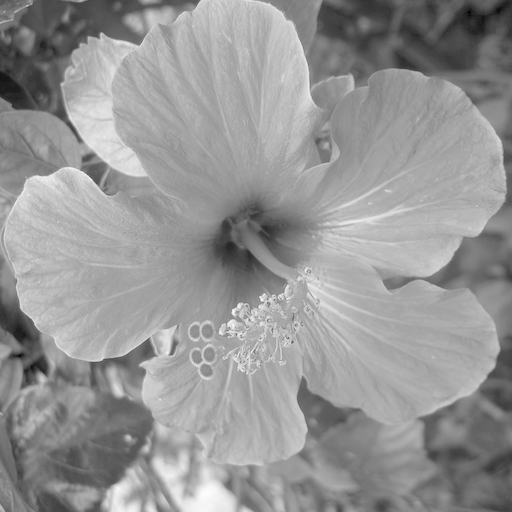
\includegraphics[width=.19\linewidth]{hist-eq/equalized-1}&
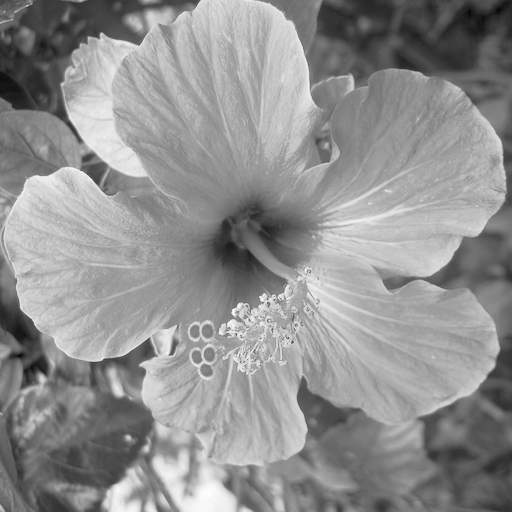
\includegraphics[width=.19\linewidth]{hist-eq/equalized-3}&
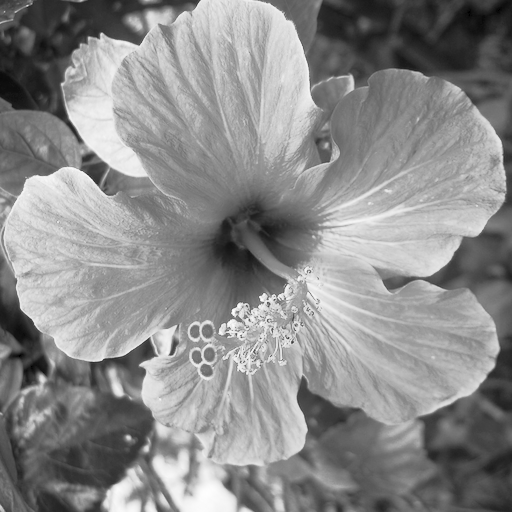
\includegraphics[width=.19\linewidth]{hist-eq/equalized-5}&
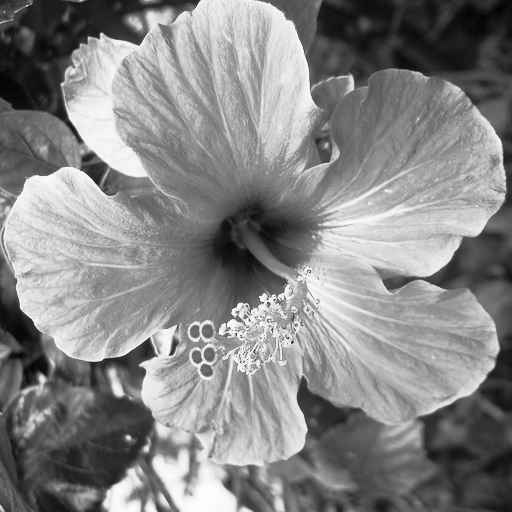
\includegraphics[width=.19\linewidth]{hist-eq/equalized-7}&
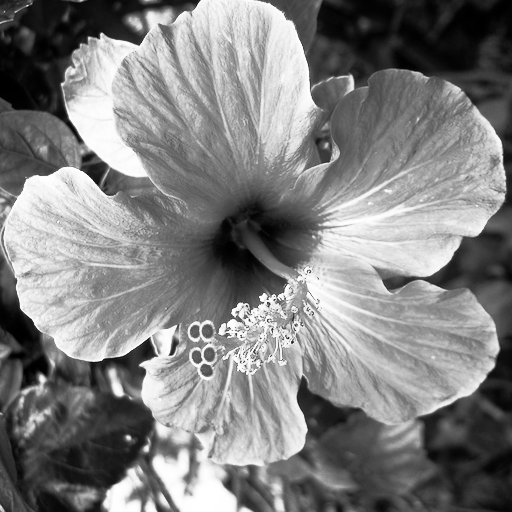
\includegraphics[width=.19\linewidth]{hist-eq/equalized-9}\\

\includegraphics[width=.19\linewidth]{hist-eq/equalize-1}&

\includegraphics[width=.19\linewidth]{hist-eq/equalize-3}&

\includegraphics[width=.19\linewidth]{hist-eq/equalize-5}&

\includegraphics[width=.19\linewidth]{hist-eq/equalize-7}&

\includegraphics[width=.19\linewidth]{hist-eq/equalize-9}\\
$t=0$ & $t=0.25$& $t=0.5$& $t=.75$& $t=1$
\end{tabular}
\caption{\label{fig-hist-eq}
画像処理のためのヒストグラム均等化。$t$はヒストグラム間の変位補間をパラメータ化する。
}
\end{figure}


%%%%%%%
\begin{rem2}{1次元の場合---一般的な場合}\label{rem-1d-ot-generic}
$\RR$上の測度$\al$に対して、$\RR$から$\rightarrow [0,1]$への累積分布関数を次のように導入する。
\eql{\label{eq-cumul-defn}
	\foralls x \in \RR, \quad \cumul{\al}(x) \eqdef \int_{-\infty}^x \d\al,
}
およびその擬逆関数$\cumul{\al}^{-1} : [0,1] \rightarrow \RR \cup \{-\infty\}$
\eql{\label{eq-pseudo-inv-cum}
	\foralls r \in [0,1], \quad \cumul{\al}^{-1}(r) = \umin{x} \enscond{x \in \RR \cup \{-\infty\} }{ \cumul{\al}(x) \geq r }.
}
%
この関数は$\alpha$の一般化分位関数とも呼ばれる。任意の$p \geq 1$に対して、次が成り立つ。
\eql{\label{eq-wass-cumul}
	\Wass_p(\al,\be)^p = \norm{ \cumul{\al}^{-1} - \cumul{\be}^{-1} }_{L^p([0,1])}^p = \int_0^1 | \cumul{\al}^{-1}(r) - \cumul{\be}^{-1}(r) |^p \d r.
}
これは、写像$\al \mapsto \cumul{\al}^{-1}$を通じて、ワッサーシュタイン距離が$L^p$ノルムを備えた線形空間と等距離であること、あるいは同値に、実数直線上の測度に対するワッサーシュタイン距離がヒルベルト的距離であることを意味する。
これにより1次元最適輸送の幾何学は非常に単純になるが、高次元のそれとは大きく異なる。高次元ではヒルベルト的ではなく、これは命題~\ref{prop-negative-definite}および\S\ref{sec-non-embeddability}でより一般的に議論される。
%
$p=1$の場合、さらに単純な公式が成り立つ。
\begin{align}\label{eq-w1-1d}
	\Wass_1(\al,\be) &= \norm{ \cumul{\al} - \cumul{\be} }_{L^1(\RR)} =
	\int_\RR | \cumul{\al}(x) - \cumul{\be}(x) | \d x \\
	&= \int_\RR \abs{ \int_{-\infty}^x \d(\al-\be) } \d x,
\end{align}
これは$\Wass_1$がノルムであることを示す（任意の次元への一般化については\S\ref{sec-w1-eucl}を参照）。
%
$\T_\sharp \al=\be$を満たす最適モンジュ写像$\T$は次で定義される。
\eql{\label{eq-OT-map-1d}
 	\T = \cumul{\be}^{-1} \circ \cumul{\al}.
}
図~\ref{fig-1d-ot}は累積関数を用いた1次元最適輸送の計算を示している。変位補間も表示されており、\eqref{eq-displacement-1d-cumul}で詳述されるように計算される。注意~\ref{rem-bary-1d}も参照されたい。1次元における最適輸送の性質の詳細な調査については、\cite[Chapter 2]{SantambrogioBook}を参照されたい。
\end{rem2}
%%%%%%%


\newcommand{\MyFigCumulMeas}[1]{\includegraphics[width=.33\linewidth]{1d-cumulative/#1}}
\newcommand{\MyFigCumulCum}[1]{\includegraphics[width=.24\linewidth]{1d-cumulative/#1}}
\begin{figure}[ht!]
\centering
\begin{tabular}{@{}c@{\hspace{1mm}}c@{\hspace{1mm}}c@{}}
\MyFigCumulMeas{input-mu}&
\MyFigCumulMeas{input-nu}&
\MyFigCumulMeas{interp-bary}\\
$\mu$ & $\nu$ & ${ (t\T+(1-t)\Id)_\sharp \mu}$
\end{tabular}
%%%%
\begin{tabular}{@{}c@{\hspace{2mm}}c@{\hspace{2mm}}c@{\hspace{2mm}}c@{}}
\MyFigCumulCum{cumul}&
\MyFigCumulCum{icumul}&
\MyFigCumulCum{transports}&
\MyFigCumulCum{interp-cumul}\\
$(\cumul{\al},\cumul{\be})$ &
$(\cumul{\al}^{-1},\cumul{\be}^{-1})$ &
$(T,T^{-1})$ &
$(1-t)\cumul{\al}^{-1}+t\cumul{\be}^{-1}$
\end{tabular}
\caption{\label{fig-1d-ot}
\eqref{eq-OT-map-1d}で詳述される累積関数を用いた、2つの1次元測度間の最適輸送と変位補間の計算。
}
\end{figure}

%%%%%%%
\begin{rem2}{ガウス分布間の距離}\label{rem-dist-gaussians}
$\al = \Nn(\mean_\al,\cov_\al)$と$\be = \Nn(\mean_\be,\cov_\be)$が$\RR^\dim$上の2つのガウス分布であるとき、次の写像
\eql{\label{eq-transport-Bures}T:x\mapsto \mean_\be + A(x-\mean_\al),}
ここで
$$A=\cov_\al^{-\tfrac{1}{2}}\Big(\cov_\al^{\tfrac{1}{2}}\cov_\be\cov_\al^{\tfrac{1}{2}}\Big)^{\tfrac{1}{2}}\cov_\al^{-\tfrac{1}{2}}=\transp{A},$$
が$T_\sharp \rho_\al = \rho_\be$を満たすことを示すことができる。実際、変数変換の公式~\eqref{eq-pfwd-density}が満たされることに注意すればよい。なぜなら
$$
\begin{aligned}\rho_\be(T(x))&=\det(2\pi\cov_\be)^{-\tfrac{1}{2}} \exp(-\dotp{T(x)-\mean_\be}{\cov_\be^{-1}(T(x)-\mean_\be)})\\
&= \det(2\pi\cov_\be)^{-\tfrac{1}{2}} \exp(-\dotp{ x-\mean_\al}{\transp{A}\cov_\be^{-1}A(x-\mean_\al)}) \\
&= \det(2\pi\cov_\be)^{-\tfrac{1}{2}} \exp(-\dotp{ x-\mean_\al}{\cov_\al^{-1}(x-\mean_\al)}),
\end{aligned}$$
であり、$T$は線形写像であるから
$$|\det T'(x)|= \det A = \left(\frac{\det\cov_\be}{\det\cov_\al}\right)^{\tfrac{1}{2}}$$
 であり、したがって$\rho_\al=|\det T'| \rho_\be$すなわち$T_\sharp \al = \be$が回復される。ここで$T$は凸関数$\psi:x\mapsto \tfrac{1}{2}\dotp{x-\mean_\al}{A (x-\mean_\al)} + \dotp{\mean_\be}{x}$の勾配であることに注目し、\citeauthor{Brenier91}の定理~\citeyearpar{Brenier91}（注意~\ref{rem-exist-mongemap}を参照）を用いて$T$が最適であると結論する。写像$T$と対応するポテンシャル$\psi$の両方が図~\ref{fig-gaussians-2d-T}と図~\ref{fig-gaussians-2d-psi}に示されている。

$\rho_\al$の1次および2次モーメントに関する追加の計算により、この写像の輸送コストは次のようになる。
\eql{\label{eq-dist-gauss}
	\Wass_2^2( \al,\be ) = \norm{ \mean_\al - \mean_\be }^2 + \Bb(\cov_\al,\cov_\be)^2,
}
ここで$\Bb$はいわゆる\citeauthor{bures1969extension}計量~\citeyearpar{bures1969extension}であり、正定値行列間で定義される（\citet{,forrester2016relating}も参照）。
\eql{\label{eq-bure-defn}
	\Bb(\cov_\al,\cov_\be)^2 \eqdef \tr\pa{
		\cov_\al + \cov_\be - 2 ( \cov_\al^{1/2} \cov_\be \cov_\al^{1/2} )^{1/2}
	},
}
ここで$\cov^{1/2}$は行列の平方根である。$\Bb$は共分散行列上の距離であり、$\Bb^2$は両引数に関して凸であることを示せる。\todoK{ref ? proof ? }
$\cov_\al = \diag(r_i)_i$および$\cov_\be = \diag(s_i)_i$が対角行列の場合、ビューレス計量はヘリンジャー距離である。
\eq{
	\Bb(\cov_\al,\cov_\be) = \norm{ \sqrt{r}-\sqrt{s} }_2.
}
1次元ガウス分布の場合、$\Wass_2$はガウス分布の平均と標準偏差$(\mean,\sqrt{\cov})$をプロットした2次元平面上のユークリッド距離となる。図~\ref{fig-1d-gaussian}に示すとおりである。
%
ガウス分布のワッサーシュタイン幾何学の詳細な扱いについては\citet{takatsu2011wasserstein}を参照されたい。ビューレス計量に関する追加の考察については、最近の文献~\citep{malago2018wasserstein,bhatia2018bures}を参照されたい。単語の確率的埋め込みを計算するためのこの計量の最近の応用については~\citep{NIPS2018_8226}を、カルマンフィルタリングのロバストな拡張を計算するための使用については~\citep{NIPS2018_8067}を、再生核ヒルベルト空間における共分散関数への適用については~\citep{NIPS2017_7149}を参照されたい。
\end{rem2}
%%%%%%
\begin{figure}[h!]
\centering

\includegraphics[width=.7\linewidth]{gaussians-2d/gaussians1.pdf}
\caption{\label{fig-gaussians-2d-T} 2つのガウス分布$\rho_\al$と$\rho_\be$。密度の等高線プロットを用いて表され、平均と分散行列はそれぞれ$\mean_\al=(-2,0),\cov_\al=\frac{1}{2}\left(1 -\tfrac{1}{2};-\tfrac{1}{2}  1\right)$および$\mean_\be=(3,1), \cov_\be=\left(2, \tfrac{1}{2}; \tfrac{1}{2}, 1\right)$である。矢印は平面上に取ったランダムな点$x$を始点とし、それらの点の対応する写像$T(x)=\mean_\be + A(x-\mean_\al)$を終点とする。}
\end{figure}



%%%%%%%
\begin{rem2}{楕円等高分布間の距離}\label{rem-dist-elliptic}
\citeauthor{gelbrich1990formula}は注意~\ref{rem-dist-gaussians}で提供されたものよりも一般的な結果を提供する。ガウス分布間のビューレス計量はより一般的に\emph{楕円等高分布}に拡張される~\citeyearpar{gelbrich1990formula}。
%
簡潔に言えば、まず、与えられた平均と共分散行列を持つ2つの測度に対して、これらのそれぞれのパラメータを持つ2つのガウス分布間の距離が2つの測度間のワッサーシュタイン距離の下界であることを示せる~\citep[Theorem 2.1]{gelbrich1990formula}。さらに、閉形式~\eqref{eq-dist-gauss}は楕円等高密度の族に拡張される。2つの密度$\rho_\al$と$\rho_\be$がそのような族に属する場合、すなわち$\rho_\al$と$\rho_\be$が平均と正定値パラメータを用いて任意の点$x$に対して次のように書ける場合、

\eq{\begin{aligned}\rho_\al(x) = \frac{1}{\sqrt{\det(\A)}}h(\dotp{x-\mean_\al}{\A^{-1}(x-\mean_\al)})\\ \rho_\be(x)= \frac{1}{\sqrt{\det(\B)}} h(\dotp{x-\mean_\be}{\B^{-1}(x-\mean_\be)}),\end{aligned}}
同一の非負値関数$h$を用いて、積分$$\int_{\RR^\dim} h(\dotp{x}{x})dx=1$$を満たすとき、それらの最適輸送写像も線形写像\eqref{eq-transport-Bures}であり、ワッサーシュタイン距離も式$\eqref{eq-dist-gauss}$で与えられる。ただし、ビューレス計量のスケーリングが生成関数$h$にのみ依存してわずかに異なる。例えば、そのスケーリングはガウス分布の場合（$h(t)=e^{-t/2}$）は$1$であり、楕円体上の一様分布の場合（$h$が$[0,1]$の指示関数）は$1/(\dim+2)$である。この結果は、楕円分布の共分散行列がその正定値パラメータの定数倍であること~\citep[Theo. 4(ii)]{gomez2003survey}と、楕円分布間のワッサーシュタイン距離がそれらの共分散行列間のビューレス距離の関数であること~\citep[Cor. 2.5]{gelbrich1990formula}から従う。
\end{rem2}
%%%%%%
\begin{figure}[h!]
\centering

\includegraphics[width=.85\linewidth]{gaussians-2d/gaussians2.pdf}
\caption{\protect\label{fig-gaussians-2d-psi} 図~\ref{fig-gaussians-2d-T}で定義されたものと同じガウス分布$\rho_\al$と$\rho_\be$。今回は曲面として表現されている。上の曲面は$T=\nabla \psi$を満たすブレニエポテンシャル$\psi$であり、加法定数の違いを除いて定義される（ここでは+50）。視覚的な目的のため、両方のガウス密度は100倍されている。}
\end{figure}

\begin{figure}[h!]
\centering
\begin{tabular}{@{}c@{\hspace{1mm}}c@{}}

\includegraphics[width=.35\linewidth]{gaussian-1d/interp-density}

\includegraphics[width=.25\linewidth]{gaussian-1d/gaussian-param}
\end{tabular}
\caption{\label{fig-1d-gaussian}
2つの1次元ガウス分布間の変位補間の計算。
%
ガウス密度を$\Gg_{m,\si}(x) \eqdef \frac{1}{\sqrt{2\pi}s}e^{-\frac{(x-m)^2}{2s^2}}$と記すと、補間$\Gg_{(1-t)m_0+t m_1,(1-t)\si_0+t \si_1}$を示す。
}
\end{figure}



\todoK{Maybe cover the case of translation / scaling of the same input. Explain that $\Wass$ is invariant to isometries. }

% !TEX root = ../ComputationalOTFnT.tex

\chapter{アルゴリズムの基礎}
\label{c-algo-basics} % a label for the chapter, to refer to it later

本章では、主問題~\eqref{eq-mk-discr}またはその双対~\eqref{eq-dual}で記述される最適輸送の離散定式化を解くために用いられる、組合せ最適化および線形計画法における最も一般的なアルゴリズム的手法について述べる。

これらのアルゴリズムの起源は第二次世界大戦にまで遡ることができ、戦前の\citeauthor{tolstoi1930methods}の先駆的な研究 \citeyearpar{tolstoi1930methods}、あるいは戦中に~\citet{Hitchcock41}および\citet{Kantorovich42}が、利用可能な資源を消費地へ最適に配分するという一般的な問題を定式化した時期に始まる。これらの定式化、および後の~\citet{koopmans1949optimum}による貢献は、いずれもその問題を解くための\emph{証明可能に}正しいアルゴリズムを提供するには至らなかった（巡回違反法は~\citet{tolstoi1939metody}によってヒューリスティックとして既に提案されていた）。線形計画法の分野が十分に成熟し、シンプレックス法が提案されるまで、これらの問題を厳密に解くことはできなかった。

線形計画法の目的は、目的関数が線形であり、制約が関心のある変数に関する線形（不）等式であるような最適化問題を解くことである。最適輸送問題はこの記述に適合するため、この広いクラスの問題の特殊な場合である。しかしながら、最適輸送はすべての線形計画の中でも真に特別であると言える。第一に、\citeauthor{dantzig1991}が線形計画を解こうとした初期の動機は、輸送問題を解くこととと密接に関連していた~\citep[p. 210]{dantzig49econometrica}。第二に、特殊な場合に過ぎないにもかかわらず、最適輸送問題は最適化の分野で注目され続けた。それは、最適輸送問題が最小費用ネットワークフローとして知られる線形計画の重要なクラスと関連し、実際には等価であることが、~\citet{ford1962flows}の結果により~\citep[p. 213, Lem. 9.3]{korte2012combinatorial}間もなく理解されたためである。そのため、OT問題は数理計画法の誕生~\citep{Dantzig51}以来、特に注目されてきており、新しい読者に最適化を紹介するために今なお広く用いられている~\citep[\S1, p. 4]{nocedal}。

\section{Kantorovichの線形計画}\label{s-kantorovich}
式~\eqref{eq-mk-discr}で主OT問題を既に導入した：
\eql{\label{eq-mk-discr-algo}
	\MKD_{\C}(\a,\b) =
	\umin{\P \in \CouplingsD(\a,\b)}
		\sum_{i\in \range{n}, j \in \range{m}} \C_{i,j} \P_{i,j}.
}
線形計画法の文献との関連を明確にするために、上記の式を\emph{標準}形の線形計画、すなわち線形目的関数、行列と定数ベクトルで定義される等式制約、および変数の非負制約を持つ線形計画として定式化できる。$\Identity_n$をサイズ$n$の単位行列、$\otimes$をクロネッカー積とする。${(n+m) \times nm}$行列
$$
\mathbf{A}= \begin{bmatrix}
	\transp{\ones_{n}} \otimes \Identity_m \\
	\Identity_n \otimes \transp{\ones_{m}}
\end{bmatrix}\in\RR^{(n+m)\times nm}
$$
は、任意の$\P$が$\CouplingsD(\a,\b)$に属するために満たすべき行和および列和の制約を符号化するために用いることができる。そのために、行列$\P\in\RR^{n\times m}$をベクトル$\p\in\RR^{nm}$として表し、$\p$の第$i+n(j-1)$要素が$\P_{ij}$に等しくなるようにする（$\P$は列方向に列挙される）と、以下の同値が得られる：
$$\P\in \RR^{n\times m}\in \CouplingsD(\a,\b) \Leftrightarrow \p\in\RR^{nm}_+, \mathbf{A}\p = \bigl[\begin{smallmatrix}\a\\ \b \end{smallmatrix} \bigr].$$
したがって、元の最適輸送問題を以下のように書くことができる：
\eql{\label{eq-mk-discr-primal}
	\MKD_{\C}(\a,\b) =
	\umin{\substack{\p \in \RR^{nm}_+\\
		\mathbf{A}\p = \bigl[\begin{smallmatrix}\a\\ \b \end{smallmatrix} \bigr]}} \transp{\cc}\p,
}
ここで$nm$次元ベクトル$\cc$はコスト行列$\C$の列を積み重ねたものに等しい。

\begin{rem}\label{rem-transportation-polytope} 上記の$n+m$個の制約のうち一つは冗長であること、言い換えれば、行列$A$の行ベクトルは線形独立ではないことに注意されたい。実際、最初の$n$行と後続の$m$行をそれぞれ足し合わせると同じベクトルが得られる（すなわち$A \bigl[\begin{smallmatrix} \ones_n\\\zeros_m \end{smallmatrix}\bigr] = A \bigl[\begin{smallmatrix} \zeros_n\\\ones_m\end{smallmatrix}\bigr]=\transp{\ones_{nm}}$）。$A$の一つの行とそれに対応する$\bigl[\begin{smallmatrix}\a\\ \b \end{smallmatrix}\bigr]$のエントリを除去しても、適切に定義された線形系が得られることが示せる。簡潔さのため、また$\a$と$\b$を非対称に扱うことを避けるため、以下では冗長な定式化を維持し、いくつかの計算で退化が生じることに留意する。\end{rem}

式~\eqref{eq-mk-discr-primal}に対応する双対問題は、線形計画法における双対性~\citep[p. 143]{bertsimas1997introduction}に従い、以下のように定義される：
\eql{\label{eq-mk-discr-dual}
	\MKD_{\C}(\a,\b) =
	\umax{\substack{\hD \in \RR^{n+m}\\
		\transp{A}\hD \leq \cc}}  \transp{\bigl[\begin{smallmatrix}\a\\ \b \end{smallmatrix} \bigr]}\hD.
}

この計画問題は式~\eqref{prop-duality-discr}で示されたものと正確に等価であることに注意されたい。


\begin{rem}\label{rem-duality} 上記の双対性の結果の簡潔な導出を示す。これは注~\ref{rem-kantorovich-dual}で展開された議論の直接的な定式化と見なすことができる。強双対性、すなわち主問題~\eqref{eq-mk-discr-primal}と双対問題~\eqref{eq-mk-discr-dual}の最適値が実際に一致するという事実は、より長い証明を要する~\citep[\S4.10]{bertsimas1997introduction}。記法を簡略化するため、$\q=\bigl[\begin{smallmatrix}\a\\ \b \end{smallmatrix} \bigr]$と書く。
ここで、最適輸送問題の緩和された主問題を考える。制約$\mathbf{A}\p=\q$はもはや必ずしも強制されず、代わりに任意のコストベクトル$\hD\in\RR^{n+m}$によってパラメータ化されたコスト$\transp{\hD}(\mathbf{A}\p-\q)$が課される。
この緩和の最適値はコストベクトル$\hD$に直接依存し、以下のように書ける：
$$\LagrangeMKD(\hD)\eqdef \umin{\p \in \RR^{nm}_+} \transp{\cc}\p-\transp{\hD}(\mathbf{A}\p-\q).$$
まず、この緩和問題は$\p$に対する周辺制約を持たないことに注意する。この最小化はより多くの$\p$の解を許容するため、$\LagrangeMKD(\hD)$は$\bar{z}=\MKD_{\C}(\a,\b)$よりも小さくなることが期待される。実際、主問題\eqref{eq-mk-discr-algo}の任意の最適解を$\p^\star$と書くと、
$$\umin{\p \in \RR^{nm}_+} \transp{\cc}\p-\transp{\hD}(\mathbf{A}\p-\q) \leq \transp{\cc}\p^\star-\transp{\hD}(\mathbf{A}\p^\star-\q)=\transp{\cc}\p^\star=\bar{z}.$$
したがって、上記のアプローチは、任意のコストベクトル$\hD$に対して元の問題~\eqref{eq-mk-discr-algo}の最適な上界を計算するための問題を定義する。この関数は$\MKD$のLagrange双対関数と呼ばれる。
双対理論の目的は、\emph{任意の}コストベクトル$\hD$に対して$\LagrangeMKD$を\emph{最大化}することにより、最良の下界$\underline{z}$を計算することである。すなわち
$$
	\underline{z}=\umax{\hD} \pa{ \LagrangeMKD(\hD)=\umax{\hD} \transp{\hD}\q + \umin{\p \in \RR^{nm}_+} \transp{(\cc-\transp{A}\hD)}\p }.
$$
$\p$に関する最小化を含む第二項は、$\transp{\cc}- \transp{A}\hD$のいずれかの座標が負であれば$-\infty$になることが容易に示される。
実際、例えばある添字$i\leq n+m$に対して$\cc_i-(\transp{A}\hD)_i<0$であれば、$\p$として正準基底ベクトル$\e_i$に任意の大きな正の値を掛けたものを取ることで、非有界な値が得られる。
下界$\LagrangeMKD(\hD)$を最大化しようとする場合、$\transp{A}\hD\leq \cc$を満たすベクトル$\hD$に制限することが合理的であり、その場合の最良の下界は$$\underline{z}=	\umax{\substack{\hD \in \RR^{n+m}\\\transp{A}\hD \leq \cc}}\transp{\hD}\q.$$となる。これにより弱双対性の結果、すなわち$\underline{z}\leq \bar{z}$が証明された。
\end{rem}


\section{$\C$変換}\label{sec-c-transforms} 本節では、双対最適輸送問題~\eqref{eq-mk-discr-dual}の重要な性質を示す。この性質は\S\ref{s-c-transform}における半離散最適輸送問題で用いる際により重要な意味を持つ。本節は、双対変数を行和と列和の制約に従って分離する元の定式化~\eqref{eq-dual}に基づいている：
\eql{\label{eq-dual-discrete-split}\MKD_\C(\a,\b) = \umax{(\fD,\gD) \in \PotentialsD(\C)} \dotp{\fD}{\a} + \dotp{\gD}{\b}.
}
任意の双対実行可能対$(\fD,\gD)$を考える。$\fD$の値を「固定」すれば、$\gD$に対する最良のベクトル解は$\fD$の$\C$変換ベクトルであることに気付く。これを$\fD^{\,\C}\in\RR^m$と書き、以下で定義される：
\eq{(\fD^{\,\C})_j = \min_{i\in \range{n}} \C_{ij}-\fD_i,}
実際、$(\fD,\fD^{\,\C})\in\PotentialsD(\C)$であること、および$\fD^{\,\C}$がこの制約を満たす最大のベクトルであることが容易に証明できる。したがって、
\eq{\dotp{\fD}{\a} + \dotp{\gD}{\b} \leq \dotp{\fD}{\a} + \dotp{\fD^{\,\C}}{\b}.}
が成り立つ。この結果により、まず双対問題を単一変数$\fD$で表される区分的アフィン凹最大化問題として再定式化できる：
\eql{\label{eq-semidual-discret}\MKD_\C(\a,\b) = \umax{\fD\in\RR^{n}} \dotp{\fD}{\a} + \dotp{\fD^{\,\C}}{\b}.}

この結果を一旦脇に置くと、$\gD$の値を「固定」して$\gD$の$\bar{\C}$変換、すなわちベクトル$\gD^{\bar{\C}}\in\RR^n$を以下で定義すれば、もちろん同じ議論が成り立つ：
\eq{(\gD^{\bar{\C}})_i = \min_{j\in \range{m}} \C_{ij}-\gD_j,}
目的関数の増加は異なり、
\eq{\dotp{\fD}{\a} + \dotp{\gD}{\b} \leq \dotp{\gD^{\bar{\C}}}{\a} + \dotp{\gD}{\b}.}
与えられた$\fD$から出発して、$\fD$を改善するために$\C$変換と$\bar{\C}$変換を複数回交互に適用したくなる。実際、以下の不等式の列が得られる：
\eq{
	\dotp{\fD}{\a} + \dotp{\fD^{\,\C}}{\b} \leq \dotp{\fD^{\,\C\bar{\C}}}{\a} + \dotp{\fD^{\,\C}}{\b}\leq  \dotp{\fD^{\,\C\bar{\C}}}{\a} + \dotp{\fD^{\,\C\bar{\C}\C}}{\b}\leq  \dots
}
これらの反復の各ステップで目的関数が真に増加することを期待するかもしれない。しかし、$\C$変換と$\bar{\C}$変換を交互に適用するとすぐに停滞するため、これはうまくいかない。

\begin{prop}\label{prop-ccc-2}以下の等式が成り立つ。ここでベクトル間の不等号は要素ごとに理解されるものとする：
	\begin{enumerate}[label=(\roman*)]
	\item $\fD\leq \fD\,' \Rightarrow \fD^{\,\C}\geq \fD\,'^{\,\C}$,
	\item $\fD^{\,\C\bar{\C}} \geq \fD$, $\gD^{\bar{\C}\C} \geq \gD$,
	\item $\fD^{\,\C\bar{\C}\C}=\fD^{\,\C}.$
\end{enumerate}
\end{prop}
\begin{proof} 第一の不等式は$\C$変換の定義から従う。$\fD^{\,\C\bar{\C}}$の定義を展開すると
\eq{\left(\fD^{\,\C\bar{\C}}\right)_i= \min_{j\in \range{m}} \C_{ij}-\fD^{\,\C}_j = \min_{j\in \range{m}} \C_{ij}- \min_{i'\in \range{n}} \C_{i'j}-\fD_{i
'}.}
ここで、$-\min_{i'\in \range{n}} \C_{i'j}-\fD_{i'} \geq -(\C_{ij}-\fD_i)$であるから、
\eq{\left(\fD^{\,\C\bar{\C}}\right)_i \geq \min_{j\in \range{m}} \C_{ij}- \C_{ij}+\fD_i = \fD_i.}
が回復される。関係式$\gD^{\bar{\C}\C} \geq \gD$も同様に得られる。次に、$\gD=\fD^{\,\C}$とおく。すると、$\gD^{\bar{\C}}=\fD^{\,\C\bar{\C}}\geq \fD$である。したがって、結果(i)を用いると$\fD^{\,\C\bar{\C}\C}\leq \fD^{\,\C}$が得られる。結果(ii)により$\fD^{\,\C\bar{\C}\C}\geq \fD^{\,\C}$であるから、等式が証明される。
\end{proof}
%Applying the $\C\bar{\C}$ transform more than once has therefore no impact.


\section{相補スラック性}\label{s-complementary}

主問題~\eqref{eq-mk-discr-primal}と双対問題~\eqref{eq-mk-discr-dual},~\eqref{eq-dual}は独立に解くことができ、最適な主変数$\P^{\star}$および双対変数$(\fD^{\star},\gD^{\star})$が得られる。以下の命題はそれらの関係を特徴づける。

\begin{prop}\label{prop-primal-dual-optimal}$\P^\star$および$\fD^\star,\gD^\star$をそれぞれ主問題~\eqref{eq-dual-generic}および双対問題~\eqref{eq-mk-discr}の最適解とする。このとき、任意の対$(i,j)\in\range{n}\times\range{m}$に対して、$\P^\star_{i,j}(\C_{i,j}-\fD^\star_i+\gD^\star_j)=0$が成り立つ。言い換えれば、$\P^\star_{i,j}>0$ならば必然的に$\fD^\star_i+\gD^\star_j=\C_{i,j}$であり、$\fD^\star_i+\gD^\star_j<\C_{i,j}$ならば必然的に$\P^\star_{i,j}=0$である。
\end{prop}
\begin{proof} 強双対性により$\dotp{\P^\star}{\C} = \dotp{\fD^\star}{\a}+\dotp{\gD^\star}{\b}$が成り立つ。$\P^\star\ones_m = \a$および$\transp{\P^\star}\ones_n = \b$であることを想起すると、
	$$\begin{aligned}\dotp{\fD^\star}{\a}+\dotp{\gD^\star}{\b} &= \dotp{\fD^\star}{\P^\star\ones_m}+\dotp{\gD^\star}{\transp{\P^\star}\ones_n}\\&=  \dotp{\fD^\star\transp{\ones_m}}{\P^\star}+\dotp{\ones_n\transp{\gD^\star}}{\P^\star},\end{aligned}$$
	となり、$$\dotp{\P^\star}{\C- \fD^\star\oplus \gD^\star}=0.$$
が得られる。$(\fD^\star,\gD^\star)$は双対制約の多面体~\eqref{eq-feasible-potential}に属するため、行列$\C- \fD^\star\oplus \gD^\star$の各要素は必然的に非負である。したがって、$\P$のすべての要素が非負であることから、上記の内積がゼロに等しいという制約は、$\P_{i,j}>0$である任意の添字対$(i,j)$に対して$\C_{i,j}-(\fD_i+\gD_j)$がゼロでなければならないこと、および$\C_{i,j}>\fD_i+\gD_j$である任意の添字対$(i,j)$に対して$\P_{i,j}=0$でなければならないことを強制する。
\end{proof}

逆の結果もまた成り立つ。まず、主問題と双対問題の二つの変数が相補的であるという概念を定義する。

\begin{defn}\label{def-complementary}
行列$\P\in\RR^{n\times m}$とベクトルの対$(\fD,\gD)$が$\C$に関して相補的であるとは、$\P_{i,j}>0$であるすべての添字対$(i,j)$に対して$\C_{i,j}=\fD_i+\gD_j$も成り立つことをいう。
\end{defn}

主変数と双対変数の実行可能な対が相補的であれば、それらが最適であると結論付けることができる。

\begin{prop}\label{prop-primal-dual-optimality} $\P$と$(\fD,\gD)$がそれぞれ主問題~\eqref{eq-dual-generic}と双対問題~\eqref{eq-mk-discr}の相補的かつ実行可能な解であるならば、$\P$と$(\fD,\gD)$はともに主最適かつ双対最適である。
\end{prop}
\begin{proof}
	弱双対性により、
$$\MKD_{\C}(\a,\b)\leq \dotp{\P}{\C}=\dotp{\P}{\fD\oplus\gD}=\dotp{\a}{\fD}+\dotp{\b}{\gD}\leq \MKD_{\C}(\a,\b)$$
が成り立ち、したがって$\P$と$(\fD,\gD)$はそれぞれ主最適および双対最適である。
\end{proof}


\todoK{
\begin{prop}[主双対関係]
	\todo{something on this?}
\end{prop}
}

\section{輸送多面体の頂点}\label{s-extremal}

凸集合の頂点または端点とは、形式的にはその集合に属する点$\mathbf{x}$であって、その集合に属する$\mathbf{y}$と$\mathbf{z}$が存在し$\mathbf{x}=(\mathbf{y}+\mathbf{z})/2$が成り立つならば、必然的に$\mathbf{x}=\mathbf{y}=\mathbf{z}$であるような点をいう。空でなく有界な実行可能集合を持つ線形計画は、その実行可能集合の頂点（または端点）で最小値を達成する~\citep[p.~65, Theo.~2.7]{bertsimas1997introduction}。主最適輸送問題~\eqref{eq-mk-discr-primal}の実行可能集合$\CouplingsD(\a,\b)$は有界であるため、最適な$\P$の探索を多面体$\CouplingsD(\a,\b)$の端点の集合に限定できる。$\CouplingsD(\a,\b)$で端点となる行列$\P$は、広範な研究の対象となってきた興味深い構造を持つ~\citep[\S8]{brualdi2006combinatorial}。その構造を記述するには、輸送問題を二部グラフの形式で表す必要がある。

\subsection{$\CouplingsD(\a,\b)$のすべての頂点の台の木構造}
$V=(1,2,\dots,n)$と$V'=(1',2',\dots,m')$を二つのノード集合とする。集合$V'$のラベルには$V$のラベルと区別するためにプライムを付ける。それらの和集合$V\cup V'$は$n+m$個のノードを持ち、それらの間のすべての$nm$本の有向辺の集合$\alledges$を$\{ (i,j'), i \in \range{n}, j\in \range{m}\}$とする（ここでは整数$j\leq m$にプライムを付けて$V'$の$j'$を構成する）。各辺$(i,j')$に対して対応するコスト値$\C_{ij}$を関連付ける。$V$と$V'$の間の完全二部グラフ$\mathcal{G}$は$(V\cup V',E)$である。輸送計画はこのグラフ上の、ソース（各ノード$i$から$\a_i$が流出する）およびシンク（各ノード$j'$に$\b_j$が流入する）制約を満たすフローであり、図~\ref{fig-simplex}に非形式的に描かれている。$\CouplingsD(\a,\b)$の端点は以下の性質を持つ~\citep[p.~338,~Theo.~8.1.2]{brualdi2006combinatorial}。

\begin{figure}[h!]
\centering

\includegraphics[width=\linewidth]{algo-basics-tree-solution/networksol}
\caption{\label{fig-simplex}
二部ネットワークフロー問題としての最適輸送問題。ここで$n=3,m=4$である。ソースヒストグラム$\a$のすべての座標は左側のソースノード$1,2,3$として描かれ、ターゲットヒストグラム$\b$のすべての座標はノード$1',2',3',4'$として描かれている。このグラフはすべてのソースノードがすべてのターゲットノードに接続され、追加の辺がないという意味で二部である。各辺$(i,j')$にはコスト$\C_{ij}$が関連付けられている。実行可能なフローが右側に表示されている。命題~\ref{prop-extremal}は、少なくとも一つの巡回$((1,1'),(2,1'),(2,4'),(1,4'))$が存在するため、このフローが端点ではないことを示している。
}
\end{figure}


\begin{figure}[h!]
\centering

\includegraphics[width=\linewidth]{algo-basics-tree-solution/tree-sol2}
\caption{\label{fig-perturb}
台のグラフに巡回を持つ解$\P$は、$\P$がそれらの平均となるような二つの実行可能解$\Q$および$\RRd$を得るために摂動でき、それにより$\P$が端点であることが否定される。
}
\end{figure}

\begin{prop}[端点解]\label{prop-extremal}
$\P$を多面体$\CouplingsD(\a,\b)$の端点とする。$S(\P)\subset \alledges$を辺の部分集合$\{(i,j'), i\in\range{n}, j\in\range{m} \text{ such that } \P_{ij}>0\}$とする。このとき、グラフ$G(\P)\eqdef (V\cup V',S(\P))$は巡回を持たない。特に、$\P$は$n+m-1$個を超える非零要素を持つことができない。
 \end{prop}
\begin{proof}
背理法による。$\P$が多面体$\CouplingsD(\a,\b)$の端点であり、その対応する辺の集合$S(\P)$（簡潔に$F$と書く）に対してグラフ$G=(V\cup V',F)$が巡回を含むと仮定する。すなわち、$k>1$と相異なる添字の列$i_1,\dots,i_{k-1}\in\range{n}$および$j_1,\dots,j_{k-1}\in\range{m}$が存在し、以下に示す辺の集合$H$が$F$の部分集合を形成する。$$H=\left\{(i_1,j_1'), (i_2,j_1'), (i_2,j_2'),\dots,(i_k,j_k'),(i_1,j_k')\right\}.$$
	ここで、$\P=(\Q+\RRd)/2$を満たす二つの実行可能行列$\Q$と$\RRd$を構成する。そのために、$H$に対応する\emph{有向}巡回$\bar{H}$、すなわち対の列$i_1\rightarrow j_1', j_1' \rightarrow i_2, i_2 \rightarrow j_2',\dots, i_k \rightarrow j_k' , j_k' \rightarrow i_1$、および基本フロー量$\varepsilon < \min_{(i,j')\in F}\P_{ij}$を考える。
	摂動行列$\E$を、その$(i,j)$要素が$i\rightarrow j' \in \bar{H}$ならば$\varepsilon$、$j\rightarrow i'\in \bar{H}$ならば$-\varepsilon$、それ以外は零であるように定義する。行列$\Q=\P+\E$と$\RRd=\P-\E$を図~\ref{fig-perturb}に示されるように定義する。$\varepsilon$が十分小さいため、$\Q$と$\RRd$のすべての要素は非負である。構成上、$\E$はすべての要素がゼロの行（もしくは列）を持つか、$i_1,\dots,i_k$（もしくは$j_1,\dots,j_k$）で添字付けられた行（もしくは列）について、一つの要素が$\varepsilon$でもう一つが$-\varepsilon$であるかのいずれかである。したがって、$\E$は$\E\ones_{m}=\zeros_{n}$かつ$\transp{\E}\ones_{n}=\zeros_{m}$を満たし、$\Q$と$\RRd$は$\P$と同じ周辺分布を持ち、よって実行可能である。最後に$\P=(\Q+\RRd)/2$であり、$\Q,\RRd\ne \P$であるから、$\P$が端点であるという事実に矛盾する。$k$個のノードを持ち巡回のないグラフは$k-1$本を超える辺を持てないため、$S(\P)$は$n+m-1$本を超える辺を持てず、したがって$\P$は$n+m-1$個を超える非零要素を持てない。
\end{proof}

\subsection{北西隅法}\label{subsec-northwest}
北西（NW）隅法は、最大$n+m$回の操作で多面体$\CouplingsD(\a,\b)$の頂点を生成するヒューリスティックである。このヒューリスティックは、次節で概説するネットワークシンプレックスのような、主変数に基づいて動作するアルゴリズムの初期化において役割を果たす。

この規則は、$\P_{1,1}$に可能な限り大きな値を与えることから始まり、$\min(\a_1,\b_1)$に設定する。各ステップにおいて、要素$\P_{i,j}$は行制約$i$、列制約$j$、または可能であれば両方を飽和させるように選ばれる。添字$i,j$は次のように更新される：第一の場合は$i$を増やし、第二の場合は$j$を増やし、第三の場合は$i$と$j$の両方を増やす。この規則は$\P_{n,m}$に値が割り当てられるまで続く。

形式的には、アルゴリズムは以下のように動作する：$i$と$j$を$1$に初期化し、$r\leftarrow\a_1,c\leftarrow \b_1$とする。$i\leq n$かつ$j\leq m$の間、$t\leftarrow \min(r,c)$、$\P_{i,j}\leftarrow t$、$r\leftarrow r-t$、$c\leftarrow s-t$とし、$r=0$ならば$i$を増やし、$i\leq n$ならば$r\leftarrow\a_i$と更新する；$c=0$ならば$j$を増やし、$j\leq n$ならば$c\leftarrow \b_j$と更新する；繰り返す。以下は$\a=[0.2,0.5,0.3]$および$\b=[0.5,0.1,0.4]$を仮定した場合のこの手順の例である：
$$\begin{aligned}\begin{bmatrix} \bullet & 0 & 0 \\ 0 & 0 & 0 \\ 0& 0 & 0\end{bmatrix} &\rightarrow \begin{bmatrix} 0.2 & 0 & 0 \\ \bullet & 0 & 0 \\ 0& 0 & 0\end{bmatrix} &\rightarrow \begin{bmatrix} 0.2 & 0 & 0 \\ 0.3 & \bullet & 0 \\ 0& 0 & 0\end{bmatrix}\\ &\rightarrow \begin{bmatrix} 0.2 & 0 & 0 \\ 0.3 &0.1 &\bullet \\ 0& 0 & 0\end{bmatrix} &\rightarrow \begin{bmatrix} 0.2 & 0 & 0 \\ 0.3 &0.1 &0.1 \\ 0& 0 & \bullet\end{bmatrix} & \rightarrow \begin{bmatrix} 0.2 & 0 & 0 \\ 0.3 &0.1 &0.1 \\ 0& 0 & 0.3\end{bmatrix}\end{aligned}$$
このヒューリスティックにより得られる一意な計画を$\NW(\a,\b)$と書く。

しかし、$\a$と$\b$の順序を任意に置換し、対応するNW隅テーブルを計算し、列と行の順序を再度反転してテーブルを$\CouplingsD(\a,\b)$に復元することで、はるかに多くのNW隅解を得られることに注意されたい：$\sigma=(3,1,2),\sigma'=(3,2,1)$とすると、$\a_\sigma=[0.3,0.2,0.5], \b_{\sigma'}=[0.4,0.1,0.5]$、および$\sigma^{-1}=(2,3,1),\sigma'=(3,2,1)$となる。以下を観察されたい：
\begin{gather*}
\NW(\a_\sigma,\b_{\sigma'}) = \begin{bmatrix} 0.3 & 0 & 0 \\ 0.1 & 0.1 & 0 \\ 0& 0 & 0.5\end{bmatrix} \in \CouplingsD(\a_\sigma,\b_{\sigma'}),\\
\NW_{\sigma^{-1}\sigma'^{-1}}(\a_\sigma,\b_{\sigma'})= \begin{bmatrix} 0 & 0.1 & 0.1 \\ 0.5 & 0 & 0 \\ 0& 0 & 0.3\end{bmatrix}\in \CouplingsD(\a,\b).
\end{gather*}

$\mathcal{N}(\a,\b)$をこの方法で生成可能なすべてのNW隅解の集合とする：
$$\mathcal{N}(\a,\b)\eqdef\{ \NW_{\sigma^{-1}\sigma'^{-1}}(r_\sigma,c_{\sigma'}), \sigma,\sigma'\in S_d\}.$$
すべてのNW隅解は、構成上、最大$n+m-1$個の非零要素を持つ。NW隅法は$\a_\sigma$と$\b_\sigma'$に対して構成上一意なテーブルを生成するが、同じテーブルを与える行・列置換の対$(\sigma,\sigma')$は指数的に多く存在し得る~\citep[p. 2]{stougie2002polynomial}。$\mathcal{N}(\a,\b)$は$\CouplingsD(\a,\b)$の端点集合の（通常は真の）部分集合を形成する~\citep[Cor. 8.1.4]{brualdi2006combinatorial}。



\section{ネットワークシンプレックスのヒューリスティックな説明}\label{s-networksimplex}

グラフ$G(\P)=(V\cup V',S(\P))$が巡回を持たない実行可能行列$\P$を考える。$\P$は$n+m-1$個以下の非零要素を持ち、命題~\ref{prop-extremal}により$\CouplingsD(\a,\b)$の頂点である。
%
命題~\ref{prop-primal-dual-optimality}に従えば、$\P$が最適であることを証明するには、実行可能（すなわち$\C-\fD\oplus\gD$が非負の要素を持つ）かつ$\P$に相補的（$S(\P)$の添字対$(i,j')$が$\C_{i,j}=\fD_i+\gD_j$を満たす）な双対解$(\fD,\gD)$を得れば十分である。
%
ネットワークシンプレックスは二つの単純な原理に基づいている：各実行可能な主解$\P$に対して相補的な対$(\fD,\gD)$を関連付けることができる。
%
その対が実行可能であれば最適に到達している。そうでなければ、$\P$を実行可能性を保ちつつ修正し、その相補的な対$(\fD,\gD)$が実行可能性に近づくように変更することを考える。

\subsection{$\P$に相補的な双対対の取得}\label{subsec-obtaining}
シンプレックス法はまず、任意の端点解$\P$に相補的な双対変数の対$(\fD,\gD)$を関連付けることから始める。これは、$S(\P)$の任意の$(i,j')$に対して$\fD_i+\gD_j$が$\C_{i,j}$に等しくなるような二つのベクトル$\fD$と$\gD$を見つけることで単純に実行される。ただし、これ自体は$(\fD,\gD)$の実行可能性を保証しないことに注意する。

\begin{figure}[h!]
	\centering
	
\includegraphics[width=\linewidth]{algo-basics-tree-solution/f_of_P}
	\caption{\label{fig-f_of_P}
	実行可能な輸送$\P$と、それに対応する辺の集合$S(\P)$およびグラフ$G(\P)$。見て分かるように、グラフ$G(\P)=(\{1,\dots,5,1',\dots,6'\},S(\P))$は森であり、木グラフの和集合として表せる。この場合は三つの木からなる。}
\end{figure}


$s$を$S(\P)$の濃度とする。$\P$が端点であるため、$s\leq n+m-1$である。$G(\P)$が巡回を持たないため、$G(\P)$は図~\ref{fig-f_of_P}に示されるように木または森（木の和集合）である。$\P$に相補的な対$(\fD,\gD)$を目指して、$n+m$個の変数に対する以下の$s$本の線形等式制約を考える：
\begin{equation}\label{eq-dual-variables}
	\begin{array}{ccc}
\fD_{i_1}+\gD_{j_1}&=&\C_{i_1,j_1}\\
\fD_{i_2}+\gD_{j_1}&=&\C_{i_2,j_1}\\
\vdots & = & \vdots\\
\fD_{i_s}+\gD_{j_s}&=&\C_{i_s,j_s},\\
\end{array}
\end{equation}
ここで$S(\P)$の要素は$(i_1,j_1'),\dots,(i_s,j_s')$と列挙されている。

$s\leq n+m-1 < n+m$であるから、上記の線形系~\eqref{eq-dual-variables}は常に不定である。この退化は、$\CouplingsD(\a,\b)$の$n+m$個の制約によるパラメータ化が$n+m$個の双対変数をもたらすことから部分的に解釈できる。注~\ref{rem-transportation-polytope}で概説されたより注意深い定式化では、$n+m-1$個の制約のみを持つ等価な定式化が得られ、したがって$n+m-1$個の双対変数となる。しかし、$s$は$n+m-1$よりも真に小さくなることもある：これは$G(\P)$が二つ以上の木の非連結和である場合に生じる。例えば、図~\ref{fig-f_of_P}では$5+6=11$個の双対変数（各ノードに一つ）があるが、これら$11$個のノード間の辺は$8$本、すなわち$(\fD,\gD)$を定義する線形方程式は$8$本しかない。したがって、この設定では$G(\P)$の連結成分の数だけ不定な双対変数が存在する。

$G(\P)$に列挙された木の一つを考える。その木がソースノード間に$k$個のノード$i_1,\dots,i_k$、ターゲットノード間に$l$個のノード$j_1',\dots,j_{l}'$を持ち、$r\eqdef k+l$ノードと$r-1$本の辺を持つとする。これは$\fD$の$k$個の変数と$\gD$の$l$個の変数に対応し、$r-1$本の線形方程式で結ばれている。不定性を解消するには、その木の根ノードを任意に選び、対応する双対変数に値$0$を割り当てればよい。そこから、幅優先探索または深さ優先探索を用いて木を走査し、その木内の他のすべての双対変数の値を決定する一連の単純な変数代入を得ることができる。これは図~\ref{fig-tree-linear-solve}に示されている。この手順を$\P$のグラフ内のすべての木に対して繰り返すことで、$\P$に相補的な双対変数の対$(\fD,\gD)$が得られる。

\begin{figure}[h!]
	\centering
	
\includegraphics[width=\linewidth]{algo-basics-tree-solution/tree-linear-solve}
	\caption{\label{fig-tree-linear-solve}
 図~\ref{fig-f_of_P}に示されたグラフ$G(\P)$の最初の木に現れる五つのノードに対応する五つの双対変数$\fD_1,\fD_2,\gD_1,\gD_2,\gD_3$は、コスト行列$\C$の対応する要素を含む四つの線形方程式で結ばれている。この系は退化しているため、その木の根を選び（この例ではノード1）、対応する変数を$0$に設定し、根から木を走査（幅優先または深さ優先）することで、残りの四つの双対変数の値を反復的に求める。}
\end{figure}

\subsection{ネットワークシンプレックスの更新}
前節で得られた双対対$(\fD,\gD)$は、すべての$i,j$に対して$\fD_i+\gD_j\leq \C_{i,j}$が成り立つという意味で実行可能である可能性がある。その場合、命題~\ref{prop-primal-dual-optimality}により最適解に到達している。そうでない場合、すなわち$\fD_i+\gD_j> \C_{i,j}$となる$i,j$が存在する場合、ネットワークシンプレックスアルゴリズムが作動する。まず、グラフ$G$を実行可能解$\P$に対応するグラフ$G(\P)$に等しく初期化し、違反辺$(i,j')$を$G$に追加する。すると二つの場合が生じ得る：
\begin{enumerate}[label={(\alph*)}]
	\item $G$が（依然として）森である場合。これは$(i,j')$が既存の二つの部分木を繋ぐ場合に生じ得る。\S\ref{subsec-obtaining}で概説したアプローチをグラフ$G$に適用して新しい相補的双対ベクトル$(\fD,\gD)$を得ることができる。この追加は$n+m$個の双対変数の不定性を一つ除去するだけであり、主変数$\P$には何ら変更をもたらさないことに注意する。$(i,j')$はグラフ$G$に入ったが$\P_{i,j}$は$0$のままであるという意味で、この更新は通常退化と呼ばれる。ただし、$G(\P)$は$G$に含まれている。

	\item $G$が巡回を持つ場合。この場合、$G$が依然として森であることを保証するために$G$から辺を除去する必要があり、同時に$\P$を修正して$\P$が実行可能かつ$G(\P)$が$G$に含まれるようにする必要がある。これらの操作はすべて、$\P_{i,j}$の値を増加させ、検出された巡回に現れる$\P$の他の要素を修正することで実行できる。その方法は、命題~\ref{prop-extremal}の証明で用いたものと非常に類似している。より正確には、その巡回を$(i_1,j_1'), (j_1',i_2), (i_2,j_2'),\dots, (i_l,j_l'),(j_l',i_{l+1})$と書く。ただし、$i_1=i_{l+1}=i$として経路が$i$で始まり$i$で終わる巡回であることを保証し、$j_1=j$として巡回が追加された辺$\{i,j\}$から正の方向に始まることを強調する。すべての「正の」辺$(i_k,j_k')$（$k\leq l$に対して）のフローを増加させ、「負の」辺$(j_k',i_{k+1})$（$k\leq l$に対して）のフローを減少させて、更新された主解$\tilde{\P}$を得る。これは以下の要素を除いて$\P$に等しい：
$$\forall k\leq l,\quad \tilde{\P}_{i_k,j_k}:= \P_{i_k,j_k}+\theta;\quad \tilde{\P}_{i_{k+1},j_k}:= \P_{i_{k+1},j_k}-\theta.$$
ここで、$\theta$はその巡回を用いて添字$i,j$で可能な最大の増加量である。$\theta$の値は、巡回により負の影響を受ける最小のフロー、すなわち$\min_{k} \P_{i_{k+1},j_k}$で制御される。この更新は図~\ref{fig-simplex-update}に示されている。$k^\star$をその最小値を達成する添字とする。次に、$G$から$(i_{k^\star+1},j_{k^\star})$を除去し、\S\ref{subsec-obtaining}で概説したアプローチを用いて新しい双対変数$(\fD,\gD)$を計算することで更新を終了する。
\end{enumerate}

\subsection{主解の改善} 必ずしも当初の動機ではなかったが、上記の操作が$\P$のコストを改善することしかできないことを示すことができる。追加された辺が巡回を生じなかった場合、すなわち上記の場合{(a)}では、主解は変更されない。巡回が生じた場合、すなわち場合{(b)}では、$\P$は$\tilde{\P}$に更新され、以下の等式が成り立つ：
\eq{
\dotp{\tilde{\P}}{\C}-\dotp{\P}{\C}= \theta \left(\;\sum_{k=1}^{l} \C_{i_k,j_k} - \sum_{k=1}^{l}\C_{i_{k+1},j_k}\right).
}
ここで、前回の反復の最後に計算された双対ベクトル$(\fD,\gD)$を用いる。これらは$\f_{i_k}+\g_{i_k}=\C_{i_k,j_k}$かつ$\f_{i_{k+1}}+\g_{i_k}=\C_{i_{k+1},j_k}$をもともと$G$にあった\emph{すべての}辺に対して満たし、以下の等式をもたらす：
\eq{
\begin{aligned}\sum_{k=1}^{l} \C_{i_k,j_k} - \sum_{k=1}^{l}\C_{i_{k+1},j_k} &= \C_{i,j} + \sum_{k=2}^{l} \fD_{i_k}+\gD_{j_k} - \sum_{k=1}^{l} \fD_{i_{k+1}}+\gD_{j_k}\\
	&= \C_{i,j} - (\fD_{i} +\gD_{j}).
\end{aligned}
}
この項は、定義上、$i,j$が$C_{i,j} < \fD_{i} -\gD_{j}$であるために選ばれたことから負である。したがって、$\theta>0$ならば、\eq{\dotp{\tilde{\P}}{\C}=\dotp{\P}{\C}+\theta\left(\C_{i,j}-(\fD_{i} -\fD_{g})\right)<\dotp{\P}{\C}.}
$\theta=0$の場合（$G$と$G(\P)$が異なる場合に生じ得る）、グラフ$G$が変更されるだけで$\P$は変化しない。


\begin{figure}[h!]
	\centering
	
\includegraphics[width=\linewidth]{algo-basics-tree-solution/simplex-update}
	\caption{\label{fig-simplex-update}
辺$\{i,j\}$をグラフ$G(\P)$に追加すると、(a) この追加後もグラフが森のままとなる場合があり、その場合は\S\ref{subsec-obtaining}で概説したアプローチに従って$\fD,\gD$を再計算できる；(b.1) この辺の追加により巡回が生じ、そこから有向経路を定義できる；(b.2) その経路を用いて$\P_{i,j}$の値を増加させ、フローの実行可能性制約を維持するためにその変更を巡回に沿って伝播させることができる。これは巡回により負の影響を受ける辺の一つのフローが$0$に減少するまで続く。これにより巡回が除去され$\P$が更新される。}
\end{figure}

したがって、ネットワークシンプレックスアルゴリズムは以下のように要約できる：\S\ref{subsec-northwest}で述べたNW隅法などにより与えられる端点解$\P$でアルゴリズムを初期化する。グラフ$G$を$G(\P)$で初期化する。\S\ref{subsec-obtaining}で述べた$G$内の木構造を用いた線形系の解法により、$\P$に相補的な双対変数の対$(\fD,\gD)$を計算する。{(i)} 制約$\C- \fD\oplus \gD\geq 0$に対する違反添字対を探す；見つからなければ$\P$は最適であり停止する。違反対$(i,j')$があれば、{(ii)} 辺$(i,j')$を$G$に追加する。$G$が依然として巡回を持たなければ、$(\fD,\gD)$をそれに応じて更新する；巡回があれば、$(i,j')$が正としてラベル付けされるように向きを付け、その巡回中の最小フロー値を持つ負の辺を除去し、図~\ref{fig-simplex-update}に示されるように$\P,G$を更新し、それに応じて相補的な対$\fD,\gD$を構築する；{(i)}に戻る。上記の操作の一部はグラフ操作（巡回検出、木走査）を必要とし、この文脈で効率的に実装できる。詳細は(\cite[\S5]{bertsekas1998network})に述べられている。

\citet{Orlin1997}がネットワークシンプレックスの多項式時間計算量を最初に証明した。\citet{Tarjan1997}はその直後に、ピボット辺の選択を支援するより効率的なデータ構造に依拠する改良された計算量$O\left(\,(n+m)nm \log(n+m)\log\left((n+m)\|\C\|_\infty\right)\,\right)$を示した。



%\paragraph{Improvement on $\P$.} Introducing a new edge $\{i,j\}$ in $G(\P)$ only because that pair violated the complementary requirement, namely because $\fD_i+\gD_j$ is strictly larger that $\C_{i,j}$, may seem like a valid approach to get closer to the goal of obtaining a feasible pair $(\fD,\gD)$ but it does not necessarily explain why this would result in a better solution $\P$ at all.

\section{双対上昇法}\label{s-dual-ascent}

双対上昇法はネットワークシンプレックスに数十年先立つものであり、\citet{borchardt1865investigando}の研究、および後に\citet{Kuhn1955}によって再述されたK\"onigとEgerv\'aryの研究にまで遡ることができる。ハンガリアン法はこの族で最もよく知られたアルゴリズムであり、$\a$と$\b$が等しくともに一様分布である特殊な場合、すなわち$\a=\b=\ones_n/n$の場合にのみ動作する。以下では、より一般的な双対上昇法の族の簡潔な説明を行う。これには最大流問題の知識が必要である(\cite[\S7.5]{bertsimas1997introduction})。上述の主問題で提示されたネットワークシンプレックスとは対照的に、双対上昇法は各反復において双対実行可能解を維持し、$\fD$と$\gD$に疎なベクトルを加えることでその目的関数値を徐々に改善する。我々の説明は主に(\cite[\S7.7]{bertsimas1997introduction})に基づいており、以下の定義から始まる。

\begin{defn} $S\subset\range{n},S'\subset\range{m}'\eqdef \{1',\dots,m'\}$に対して、$\ones_S$を$S$に列挙される添字で$1$、それ以外で$0$の$\RR^n$のベクトル、同様に$\ones_{S'}$を$S'$の添字を持つ$\RR^m$のベクトルと書く。
\end{defn}

以下では、$(\fD,\gD)$を$\PotentialsD(\C)$の実行可能な双対対とする。これは、すべての対$(i,j')\in\range{n}\times\range{m}'$に対して$\fD_i+\gD_j\leq\C_{ij}$が成り立つことを意味する。$(i,j')$が$\fD_i+\gD_j=\C_{ij}$のとき\emph{均衡}対（または辺）と呼び、$\fD_i+\gD_j<\C_{ij}$のとき\emph{非活性}と呼ぶ。この規約のもと、実行可能な双対対$(\fD,\gD)$が集合$S$と$S'$で添字付けられた疎なベクトルを用いて摂動されても実行可能であり続ける条件を記述する簡単な結果から始める。

\begin{prop}\label{prop-feasibility-dual-pair}
$(\tilde{\fD},\tilde{\gD})\eqdef(\fD,\gD)+\varepsilon(\ones_S,-\ones_{S'})$が十分小さい$\varepsilon>0$に対して双対実行可能であるための条件は、すべての$i\in S$に対して$(i,j')$が均衡であれば$j'\in S'$であることである。
\end{prop}
\begin{proof}
任意の$i\in S$に対して、$(i,j')$が非活性であるすべての$j'\in\range{m}'$、すなわち$\fD_i+\gD_j<\C_{ij}$であるすべての$j'$の集合$\mathcal{I}_{i}$を考える。$\varepsilon_i \eqdef \min_{j\in I_{i}} \C_{i,j}-\fD_i-\gD_j$を、$j'\in \mathcal{I}_i$に対応する制約を違反することなく$\fD_i$を増加させることのできる最小のマージンと定義する。実際、$\varepsilon\leq \varepsilon_i$ならば任意の$j'\in \mathcal{I}_i$に対して$\tilde{\fD}_i+\tilde{\gD}_j<\C_{i,j}$が成り立つ。次に、$i$に関連する均衡辺の集合$\mathcal{B}_i$を考える。$\mathcal{B}_i=\range{m}'\setminus \mathcal{I}_i$であることに注意する。上記の仮定は$j'\in\mathcal{B}_i\Rightarrow j'\in S'$である。したがって、$j'\in\mathcal{B}_i$に対して$\tilde{\fD}_i+\tilde{\gD}_j=\fD_i+\gD_j=\C_{i,j}$が成り立つ。結果として、不等式$\tilde{\fD}_i+\tilde{\gD}_j\leq \C_{i,j}$は任意の$j\in \range{m}'$に対して保証される。許容される最小の増加量、すなわち$\min_{i\in S} \varepsilon_i$よりも小さい増加$\varepsilon$を選ぶと、$(\tilde{\fD},\tilde{\gD})$が双対実行可能であることが回復される。
\end{proof}

\S\ref{subsec-obtaining}で示したネットワークシンプレックスの反復の主な動機は、実行可能な主解$\P$から出発して相補的な実行可能双対対$(\fD,\gD)$を得ることである。その目標を達成するため、$\P$はその相補的双対対が双対実行可能性に到達するよう徐々に修正される。対称的なアプローチ、すなわち実行可能な双対変数から出発して実行可能な主変数$\P$を得るアプローチが、双対上昇法の動機となっている。以下の命題は双対上昇法の主要なエンジンであり、$(\fD,\gD)$に対して実行可能性を維持する上昇方向の存在を（構成的に）保証する。その方向は、ネットワークシンプレックスと同様に、候補の主解$\P$を設計し、その非実行可能性が$(\fD,\gD)$の更新を導くことで構築される。

\begin{prop}\label{prop-dual-ascent-dir} $(\fD,\gD)$が問題~\eqref{eq-dual-discrete-split}に対して最適であるか、または$S\subset\range{n},S'\subset\range{m}'$が存在して$(\tilde{\fD},\tilde{\gD})\eqdef(\fD,\gD)+\varepsilon(\ones_S,-\ones_{S'})$が十分小さい$\varepsilon>0$に対して実行可能でありかつ真に良い目的関数値を持つかのいずれかである。
\end{prop}
\begin{proof}
まず、$(\fD,\gD)$に相補的な主変数$\P$を考える。そのために、均衡辺の集合$\mathcal{B}$、すなわち$\fD_i+\gD_j=\C_{i,j}$であるすべての対$(i,j')\in\range{n}\times\range{m}'$を定め、頂点$\{1,\dots,n,1',\dots,m'\}$が$\mathcal{B}$の辺のみで結ばれた二部グラフを形成する。これに、ソースノード$s$をすべてのノード$i\in\range{n}$に\emph{容量制限付き}辺（容量$\a_i$）で接続し、ターミナルノード$t$をすべてのノード$j'\in\range{m}'$に容量$\b_j$の辺で接続して補完する。図~\ref{fig-dualascent}に示される通りである。Ford--Fulkersonアルゴリズム(\cite[p. 305]{bertsimas1997introduction})をこのネットワークに適用して最大流$\mathbf{F}$を計算できる。すなわち、$(i,j')\in \mathcal{B}$で添字付けられる$n+m+|\mathcal{B}|$個の非負値の族$f_{si}\leq \a_i, f_{ij'}, f_{j't}\leq\b_j$で、流量保存制約を満たし$\sum_i f_{si}$が最大であるものを求める。この流$\mathbf{F}$のスループットが$1$に等しければ、$\fD,\gD$に構成上相補的な実行可能主解$\P$が$\mathbf{F}$から抽出でき、$(i,j')\in \mathcal{B}$に対して$\P_{i,j}=f_{ij'}$、それ以外では零と定義する。これにより命題~\ref{prop-primal-dual-optimality}から$(\fD,\gD)$と$\P$の最適性が得られる。$\mathbf{F}$のスループットが$1$より真に小さい場合、ラベリングアルゴリズムは$s$から反復的に到達可能で$\mathbf{F}$が容量制約を飽和させないノード、およびラベル付けされたノードにフローを供給するノードをラベル付け（識別）する。ラベル付けされたノードは空でない集合$Q$に格納され、$\mathbf{F}$の最適性によりターミナルノード$t$は含まれない（厳密な提示は\citealt[p. 308]{bertsimas1997introduction}を参照）。$Q$は二つの集合$S=Q\cap\range{n}$と$S'=Q\cap\range{m}'$に分割できる。総スループットが$1$より真に小さいと仮定しているため、$S\ne\emptyset$である。まず、$i\in S$かつ$(i,j)$が均衡であれば、$j'$は必然的に$S'$に属することに注意する。実際、すべての辺$(i,j')$は構成上無限容量を持つため、ラベリングアルゴリズムは$i$を$S$に含めると必然的に$j'$にも到達する。命題~\ref{prop-feasibility-dual-pair}により、$\tilde{\fD},\tilde{\gD}$の実行可能性を保証する十分小さい$\varepsilon$が存在する。$(\tilde{\fD},\tilde{\gD})$が$(\fD,\gD)$よりも良い目的関数値を持つことを保証するためには、$\transp{\ones_S}{\a}-\transp{\ones_{S'}}{\b}>0$を証明する必要がある。$\bar{S}=\range{n}\setminus S$、$\bar{S'}=\range{m}'\setminus S'$とし、
$$A = \sum_{i\in S} f_{si}, \quad B = \sum_{i\in \bar{S}} f_{si}, \quad C = \sum_{j'\in S'} f_{j't}, \quad D = \sum_{j'\in \bar{S'}} f_{j't}.$$
と定義する。総最大流は$s$から出発するため$A+B$に等しく、同時に$t$に到着するため$C+D$にも等しい。流量保存制約により、同じ流はまた$B+C$にも等しく、したがって$A=C$である。一方、ラベリングアルゴリズムの定義により、$S$のすべての$i$に対して$f_{si}<\a_i$であり、$\bar{S}'$の$j'$に対しては$t$が最適流により$S'$に含まれないため$f_{j't}=\b_j$である。したがって$A<\transp{\ones_S}\a$かつ$C=\transp{\ones_S'}\b$である。よって$\transp{\ones_S}\a-\transp{\ones_S'}\b>A-C=0$が成り立つ。
\end{proof}

\begin{figure}[h!]
\centering

\includegraphics[width=\linewidth]{algo-basics-tree-solution/dual_ascent}
\caption{\label{fig-dualascent}
図~\ref{fig-f_of_P}で最初に導入した周辺分布を含む輸送問題を考える。$n=5, m=6$である。二つの実行可能な双対ベクトル$\fD,\gD$が与えられたとき、$(\fD,\gD)$に相補的な「最良の」フロー行列$P$を求めようとする。これは$\P$が$\fD_i+\gD_j=\C_{i,j}$となる添字に対応する辺$(i,j')$でのみ正の値を取れることを意味する。これはプロット(a)で点線で表されている。そのグラフ構造で達成できる最良のフローは、抽象的なソースノード$s$から$i\in\range{n}$とラベル付けされたすべてのノードへの辺、抽象的なターミナルノード$t$から$j\in\range{m'}$の$j'$とラベル付けされたすべてのノードへの辺を持つ容量制限付きネットワークにおける最大流問題として定式化できる。ここで辺$(s,i),(j',t), i\in \range{n},j\in\range{m}$の容量はそれぞれ$\a_i,\b_j$であり、他はすべて無限である。Ford--Fulkersonアルゴリズム(\cite[p. 305]{bertsimas1997introduction})を適用してそのような最大流を計算できるが、プロット(b)に示されるように、問題を解くために必要な$1$単位の質量のうち$0.74$単位しか達成できない。最大流アルゴリズムで使われるサブルーチンの一つであるラベリングアルゴリズム(\cite[p. 308]{bertsimas1997introduction})を用いて、$s$から飽和していないフローを受け取るノード（および再帰的にそのすべての後続ノード）を識別でき、プロット(c)ではオレンジの線で示されている。ラベリングアルゴリズムはまた、ラベル付けされたノードに正のフローを送るノードもデフォルトで追加する。この基準によりノード$3$が選択され、$3'$への赤い線で示されている。ラベル付けされたノードは集合$S,S'$にグループ化でき、$\fD,\gD$を変更して異なるグラフを得ることで、より高いフローを得るためにより良く活用できるノードを識別する。証明にはプロット(d)に記述された部分フロー和が関わる。}
\end{figure}

双対上昇法は、実行可能性を保証し目的関数を改善する集合$S,S'$により生成される任意のベクトルで実行可能解$(\fD,\gD)$を修正することで進む。集合$S,S'$が命題~\ref{prop-dual-ascent-dir}の証明で構成的に与えられたものであり、ステップ長$\varepsilon$が命題~\ref{prop-feasibility-dual-pair}の証明で定義されたものである場合、\emph{主双対法}として知られる方法が回復される。この方法はマッチング問題に対してはハンガリアン法に帰着される。双対上昇法はネットワークシンプレックスの双対変形と類似点を持つが、少なくとも二つの重要な点で異なる。シンプレックス型の方法は、現在の解が常に実行可能集合の\emph{端点}（双対の場合は$\PotentialsD(\C)$）であることを保証するが、ここで提示された双対上昇法はそのような仮定を置かず、実行可能集合の内部にある反復点を自由に生成できる。さらに、双対ネットワークシンプレックスが$(\fD,\gD)$を修正して線形（周辺制約）を満たす主解$\P$を生成し、非負性は収束時にのみ満たされるのに対して、双対上昇法は常に非負であるが必ずしも周辺制約を満たさない主解$\P$を構築する。

\section{競売アルゴリズム}\label{s-auction}
競売アルゴリズムは~\citet{bertsekas1981new}によって最初に提案され、後に~\citep{bertsekas1988dual}で改良された。このアルゴリズムにはいくつかの経済学的解釈が提案されている（例えば\citet{bertsekas1992auction}を参照）。このアルゴリズムは任意の周辺分布に対して適用可能であるが、ここでは最適割当問題を解くための定式化で提示する。

\paragraph{相補スラック性。} 最適割当問題では、最適輸送問題に対して示した主双対条件がより定式化しやすくなることに注意する。任意の端点解$\P$は\todoK{there always exist a permutation solution, but the converse it not true}必然的にある$\si$に対する置換行列$\P_\si$である（式~\eqref{prop-primal-dual-optimality}を参照）。最適な主変数$\P_{\si^\star}$と双対変数$\fD^\star,\gD^\star$が与えられると、
$$
\fD^\star_i + \gD^\star_{\si^\star_i} = \C_{i,{\si_i^\star}}.
$$
が必然的に成り立つ。また、\S\ref{sec-c-transforms}で述べた$\C$変換の原理により、$\fD^\star$は$\gD^{\bar\C}$に等しく選ぶことができることを想起されたい。したがって、
\eql{\label{eq-dual-conditions-assign-1}
\C_{i,\si^\star_i} - \gD^\star_{\si_i}  = \min_{j} \C_{i,j} - \gD^\star_{j}.
}
逆に、あるベクトル$\gD$と置換$\sigma$が存在して
\eql{\label{eq-dual-conditions-assign}
\C_{i,\si_i} - \gD_{\si_i}  = \min_{j} \C_{i,j} - \gD_{j}
}
が成り立つならば、それらはともに最適であること、すなわち$\si$が最適割当であり$\gD^{\bar\C},\gD$が最適双対対であることが容易に示される。


\paragraph{部分割当と$\varepsilon$-相補スラック性。} 競売アルゴリズムの目標は、三つ組$S,\xi,\gD$を反復的に修正することである。ここで$S$は$\range{n}$の部分集合、$\xi$は部分割当ベクトル（$S$から$\range{n}$への単射）、$\gD$は双対ベクトルである。双対ベクトルは\emph{近似的な}相補スラック性~\eqref{eq-dual-conditions-assign}を満たす解に収束することを意図しており、$S$は$\xi$が置換を記述するにつれて$\range{n}$を覆うように成長する。アルゴリズムは各反復後に以下の三つの性質を維持することで動作する：
\begin{enumerate}[label={(\alph*)}]
	\item $\forall i\in S,\quad \C_{i,\xi_i} - \gD_{\xi_i}  \leq \varepsilon + \min_{j} \C_{i,j} - \gD_{j}$（$\varepsilon$-CS）。
	\item $S$のサイズは各反復で増加することしかできない。
	\item ある添字$i$が存在して$\gD_i$が少なくとも$\varepsilon$だけ減少する。
\end{enumerate}

\paragraph{競売アルゴリズムの更新。} 点$j$が与えられると、競売アルゴリズムは通常の$\C$変換に現れる最適値だけでなく、二番目に良い値も使用する：
$$j^1_i \in \argmin_{j} \C_{i,j} - \gD_{j}, \quad j^2_i \in \argmin_{j\ne j^1_i} \C_{i,j} - \gD_{j}, $$
以下の更新を、$i\notin S$である添字$i$に対する$\gD$の更新、および$S$と$\xi$の更新として定義する：
\begin{enumerate}\item \textbf{$\gD$の更新}：$\gD$の第$j^1_i$要素から、$\varepsilon$と調整コスト$\{\C_{i,j}-\gD_j\}_j$の最低値と二番目の最低値の差の和を引く：
\eql{
\begin{aligned}
	\gD_{j^1_{i}} &\leftarrow \gD_{j^1_{i}} - \underbrace{\left((\C_{i,j^2_{i}}-\gD_{j^2_{i}})-(\C_{i,j^1_{i}}-\gD_{j^1_{i}})+\varepsilon\right)}_{\geq \varepsilon >0}\label{eq-auction-update}\\
	&= \C_{i,j^1_{i}} - (\C_{i,j^2_{i}}-\gD_{j^2_{i}}) -\varepsilon.\\
\end{aligned}
}
\item \textbf{$S$と$\xi$の更新}：$\xi_{i'}=j^1_{i}$となる添字$i'\in S$が存在すれば、$S\leftarrow S\setminus \{i'\}$として除去する。$\xi_{i}=j^1_{i}$と設定し、$i$を$S$に追加する。$S\leftarrow S \cup \{i\}.$
\end{enumerate}

\paragraph{アルゴリズムの性質。} アルゴリズムは割当点の空集合$S=\emptyset$、割当なし、空の部分割当ベクトル$\xi$、および$\gD=\zeros_n$から開始し、$S=\range{n}$で終了し、終了するまで上記の両ステップを繰り返す。性質{(b)}と{(c)}が各反復後に成り立つことは、更新の性質から明らかである（式~\eqref{eq-auction-update}を見れば十分である）。$\varepsilon$-相補スラック性は最初の反復で容易に満たされる。この場合$S=\emptyset$であるためである。反復がこの性質を保存するという事実は以下の命題で示される。
%Show::: $(\fD^{\,\tau})_i < (\fD^{\,\C\bar{\C}})_i$
\begin{prop} 競売アルゴリズムは各反復において$\varepsilon$-相補スラック性を維持する。
\end{prop}
\begin{proof}
	$\gD,\xi,S$をある反復の開始時の三つの変数とする。したがって、任意の$i'\in S$に対して
	$$\C_{i,\xi_{i'}} - \gD_{\xi_{i'}}  \leq \varepsilon + \min_{j} \C_{{i'},j} - \gD_{j} $$
が成り立つと仮定する。ここで反復で考慮される特定の$i\notin S$を考える。三つの更新が行われる：$\gD,\xi,S$は添字$j^1_i$と$j^2_i$を用いて$\gD^{\text{n}},\xi^{\text{n}},S^{\text{n}}$に更新される。より正確には、$\gD^{\text{n}}$は要素$j^1_i$を除いて$\gD$に等しく、その値は
$$\gD_{j^1_{i}}^\text{n} = \gD_{j^1_{i}} - \left((\C_{i,j^2_{i}}-\gD_{j^2_{i}})-(\C_{i,j^1_{i}}-\gD_{j^1_{i}})\right)-\varepsilon \leq \gD_{j^1_{i}}-\varepsilon$$,
$\xi^{\text{n}}$は第$i$要素が$j^1_i$に等しい点を除いて$\xi$に等しく、$S^{\text{n}}$は$\{i\}$と$S$の和集合に等しい（一つの要素が除去される可能性がある）。$\gD^{\text{n}}$の更新は次のように書き直せる：
$$\gD^{\text{n}}_{j^1_i}= \C_{i,j^1_{i}} - (\C_{i,j^2_{i}}-\gD_{j^2_{i}}) -\varepsilon;$$
したがって
$$\C_{i,j^1_{i}} - \gD^{\text{n}}_{j^1_i}=  \varepsilon + (\C_{i,j^2_{i}}-\gD_{j^2_{i}}) = \varepsilon+\min_{j\ne j^1_i} (\C_{i,j}-\gD_{j}).$$
$-\gD\leq -\gD^{\text{n}}$であるから、
$$\C_{i,j^1_{i}} - \gD^{\text{n}}_{j^1_i} = \varepsilon + \min_{j\ne j^1_i} (\C_{i,j}-\gD_{j})\leq \varepsilon+\min_{j\ne j^1_i} (\C_{i,j}-\gD^{\text{n}}_{j}),$$
が得られ、$j=j^1_i$に対しても不等式は明らかに成り立つため、添字$i$に対する$\varepsilon$-相補スラック性が得られる。他の添字$i'\ne i$に対しては、同様に$\gD^{\text{n}}\leq\gD$であるから、以下の不等式の列が成り立つ：
$$\C_{i,\xi^{\text{n}}_{i'}} - \gD^{\text{n}}_{\xi^{\text{n}}_{i'}} = \C_{i,\xi_{i'}} - \gD_{\xi_{i'}} \leq \varepsilon + \min_{j} \C_{{i'},j} - \gD_{j} \leq \varepsilon + \min_{j} \C_{{i'},j} - \gD^{n}_{j}. $$
\end{proof}

\begin{prop} 競売アルゴリズムのステップ数は最大$N=n\|\C\|_\infty/\varepsilon$である。
\end{prop}
\begin{proof}アルゴリズムが$T>N$ステップ後に停止していないと仮定する。すると、$\xi$の像に含まれない添字$j$が存在し、その価格座標$\gD_j$は一度も更新されず$\gD_j=0$のままである。この場合、$n>\|\C\|_\infty/\varepsilon$回更新された添字$j'$は存在し得ない。実際、もしそうであれば任意の添字$i$に対して
$$\gD_{j'}\leq-n\varepsilon<-\|\C\|_\infty\leq -\C_{i,j} = \gD_j-\C_{i,j},$$
が成り立ち、すべての$i$に対して
$$\C_{i,j'}-\gD_{j'}> \C_{i,j}+ (\C_{i,j}-\gD_j),$$
となるが、これは$\varepsilon$-CSに矛盾する。したがって、各変数の更新回数は$\|C\|_\infty/\varepsilon$を超えないため、総反復回数$T$は$n\|\C\|_\infty/\varepsilon=N$を超えることができない。
\end{proof}

\begin{rem} この結果は、アルゴリズムが終了するための素朴な演算回数として$N^3\|\C\|_\infty/\varepsilon$を与えることに注意されたい。この計算量は、$\varepsilon$の値を各反復で減少させる巧妙な方法である$\varepsilon$スケーリングを用いることで$N^3 \log\|\C\|_\infty$に削減できる(\cite[p. 264]{bertsekas1998network})。
\end{rem}

\begin{prop} 競売アルゴリズムは、コストが$n\varepsilon$だけ準最適な割当を見つける。
\end{prop}
\begin{proof}
	$\sigma,\gD^\star$をコスト行列$\C$の割当問題の主および双対最適解とし、最適値を$$t^\star=\sum \C_{i,\sigma_i} = \sum_i \min_{j}\C_{i,j}-\gD^\star_j+\sum_j\gD^\star_j.$$とする。
$\xi,\gD$を終了時に競売アルゴリズムが出力する解とする。$\varepsilon$-CS条件により、任意の$i\in S$に対して
$$\min_{j} \C_{i,j} - \gD_{j}\geq \C_{i,\xi_i} - \gD_{\xi_i} -\varepsilon.$$
が成り立つ。したがって、$\gD$の準最適性によりまず
	$$\begin{aligned}t^\star&\geq \sum_i \left(\min_{j} \C_{i,j}-\gD_{j}\right) + \sum_j \gD_j\\
&\geq
	\sum_i -\varepsilon+\left(\C_{i,\xi_i}-\gD_{\xi_i}\right) + \sum_j \gD_j = -n\varepsilon + \sum_i \C_{i,\xi_j} \geq  - n\varepsilon + t^\star.\end{aligned},$$
が得られる。ここで第二の不等式は$\varepsilon$-CSから、次の等式は$\gD_{\xi_i}$の項と$\gD_{j}$の和の打消しから、最後の不等式は置換としての$\xi$の準最適性から従う。
\end{proof}


したがって、競売アルゴリズムは$\C$変換の機構を利用する別の方法と見なすことができる。次に、正則化に基づく別のアプローチ、いわゆるSinkhornアルゴリズムを探究する。これは~\citep{schmitzer2016stabilized}で議論されているように、競売アルゴリズムとも類似点がある。
% $\fD^{\,\C\bar{\C}\C}\geq \fD^{\,\C}$ implies that $\fD^{\,\C\bar{\C}\C\bar{\C}}\leq \fD^{\,\C\bar{\C}}$
%

最後に、Euclid空間の低次元正則格子上では、これらの古典的な線形ソルバーにマルチスケール戦略を組み合わせることで、大幅な高速化が可能であることを注記する~\citep{schmitzer2016sparse,oberman2015efficient}。




%\section{Interior point methods}\label{s-ipm}
% \begin{rem}\label{rem:duality}Recall that a simple argument can help us recover the dual problem from the primal. For convenience, let us write $\q=\bigl[\begin{smallmatrix}\a\\ \b \end{smallmatrix} \bigr]$.
% 	Let $\U$ be the feasible set $\{\p\in\mathbb{R}^{nm}, \mathbf{A}\p = \q\}$.
% 	The feasible set's indicator function $\iota_\U$, such that $\iota_{\U}(\p)=0$ if $\p\in \U$ and $\infty$ otherwise,
% 	can be written as $\max_{\hD\in\mathbb{R}^{n+m}} -\hD^T(\mathbf{A}\p-\q)$.
% 	Indeed, the optimal value of that problem is obviously 0 when $\p$ is such that $\mathbf{A}\p=\q$, and $\infty$ otherwise, since it suffices to take for $\hD$ any negative constant that is large enough, and multiply it by vector $\mathbf{A}\p-\q$ to obtain an arbitrarily large objective value. Therefore, using the extended definition of convex functions, we have that
% $$\begin{aligned}
% \umin{\substack{\p \in \RR^{nm}_+\\\mathbf{A}\p = \q}} \cc^T\p & = \umin{\p \in \RR^{nm}_+} \cc^T\p + \iota_S(\p) =\umin{\p \in \RR^{nm}_+} \cc^T\p + \max_{\hD\in\mathbb{R}^{n+m}} -\hD^T(\mathbf{A}\p-\q)
% \\ & = \umin{\p \in \RR^{nm}_+}  \max_{\hD\in\mathbb{R}^{n+m}}  \cc^T\p - \hD^T(\mathbf{A}\p-\q)
% \\ & = \max_{\hD\in\mathbb{R}^{n+m}} \hD^T\q + \umin{\p \in \RR^{nm}_+} (\cc-\transp{\mathbf{A}}\hD)^T\p.
% \end{aligned}$$
% where we have assumed in the third line that one can inverse the orders of $\min$ and $\max$ problems. One can also notice that the term $\umin{\p \in \RR^{nm}_+} (\cc-\transp{\mathbf{A}}\hD)^T\p$ is minus the indicator function of the set $\R=\{\hD, \transp{\mathbf{A}}\hD\leq \cc\}$. Indeed, if any element of vector $\transp{\mathbf{A}}\hD$ is strictly bigger than $\cc$, say at index $i$, then the $i$-th element of $\cc-\transp{\mathbf{A}}\hD$ is negative, and it suffices to take for $\p$ the null vector except for its $i$-th index with an arbitrary large value to obtain and arbitrarily small value for the minimum. Therefore we have that
% $$
% \umin{\substack{\p \in \RR^{nm}_+\\\mathbf{A}\p = \q}} \cc^T\p = \max_{\hD\in\mathbb{R}^{n+m}} (\transp{\mathbf{A}}\hD)^T\q -\iota_{\R}(\hD)= \max_{\substack{\hD\in\mathbb{R}^{n+m}\\ \transp{\mathbf{A}}\hD\leq \cc}}\hD^T\q
% $$
% For a thorough and rigorous duality argument we refer the reader to~\cite[\S4.3]{bertsimas1997introduction}:
% \end{rem}

% !TEX root = ../ComputationalOTFnT.tex

\chapter{最適輸送のエントロピー正則化}
\label{c-entropic}

この章では、最適輸送のカントロビッチ定式化とその多くの一般化に対する近似解を求めるための数値スキームの族を導入する。これはもとの問題にエントロピー正則化ペナルティを加えることで動作する。この正則化にはいくつかの重要な利点があり、それらを総合すると非常に有用なツールとなる：正則化された問題の最小化は単純な交互最小化スキームで解くことができる；そのスキームは単純な行列-ベクトル積の反復に帰着し、GPU上での実行に特に適している；一部の応用では、これらの行列-ベクトル積は$n\times m$のコスト行列を格納する必要がなく、カーネル評価へのアクセスのみを必要とする；大規模な測度群が同じ台を共有する場合、これらの行列-ベクトル積はすべて行列-行列積として実行でき、大幅な高速化が得られる；得られる近似距離は入力ヒストグラムの重みとDirac測度の位置に関して滑らかであり、自動微分を用いて微分可能である。

%%%%%%%%%%%%%%%%%%%%%%%%%%%%%%%%%%%%%%%%%%%
\section{エントロピー正則化}

カップリング行列の離散エントロピーは次のように定義される
\eql{\label{eq-discr-entropy}
	\HD(\P) \eqdef -\sum_{i,j} \P_{i,j} (\log(\P_{i,j})-1),
}
ベクトルに対しても同様の定義が成り立ち、$\a_j$のいずれかの成分が0または負の場合は$\HD(\a) = -\infty$とする規約を設ける。関数$\HD$は1-強凹関数である。なぜならそのHesse行列は$\partial^2 \HD(P)=-\diag(1/\P_{i,j})$であり$\P_{i,j} \leq 1$だからである。最適輸送のエントロピー正則化のアイデアは、$-\HD$を正則化関数として用い、もとの輸送問題~\eqref{eq-mk-discr}の近似解を得ることである：
\eql{\label{eq-regularized-discr}
	\MKD_\C^\varepsilon(\a,\b) \eqdef
	\umin{\P \in \CouplingsD(\a,\b)}
		\dotp{\P}{\C} - \varepsilon \HD(\P).
}
目的関数は$\varepsilon$-強凸関数であるため、問題(\ref{eq-regularized-discr})は一意の最適解を持つ。最適輸送問題をエントロピー項で正則化するというアイデアは、交通理論におけるモデリングのアイデアにまで遡ることができる~\citep{wilson1969use}：ネットワークにおける実際の交通パターンは、最適輸送問題の解によって予測されるものとは一致しない。実際、後者は~\eqref{eq-mk-discr}の最適カップリングのスパース性の結果として少数のルートに依存する傾向があるのに対し、前者はより拡散的である。このスパース性を緩和するために、交通の研究者は「重力」モデル~\citep{erlander1980optimal}と呼ばれるモデルを提案し、周辺分布と輸送コストが与えられた場合に、より「ぼやけた」交通予測を形成できるようにした。

図~\ref{fig-impact-eps}は、単体$\simplex_3$（したがって2次元の三角形として可視化できる）上の線形計画法を正則化するエントロピーの効果を示している。エントロピーがもとのLP解を三角形の境界から押し離す様子に注目されたい。最適な$\P_\varepsilon$は徐々に三角形の「エントロピー的中心」に向かって移動する。これは以下の命題でさらに詳しく述べる。正則化された問題の解がもとの線形計画法の最適解に収束することは~\citet{CominettiAsympt}によって研究されており、精密な漸近展開が与えられている。


\begin{figure}[h!]
\centering

\includegraphics[width=.7\linewidth]{entropic/simplex}
\caption{\label{fig-impact-eps}
単体上の線形関数の最適化に対する$\varepsilon$の影響、様々な$\varepsilon$に対して$\P_\varepsilon = \argmin_{\P \in \simplex_3} \dotp{\C}{\P}-\varepsilon\HD(\P)$を解く。
}
\end{figure}


\begin{prop}[$\varepsilon$に関する収束]\label{prop-convergence-eps}
~\eqref{eq-regularized-discr}の一意の解$\P_\varepsilon$は、カントロビッチ問題のすべての最適解の集合の中で最大エントロピーを持つ最適解に収束する。すなわち
\eql{\label{eq-entropy-conv-1}
	\P_\varepsilon \overset{\varepsilon \rightarrow 0}{\longrightarrow}
	\uargmin{\P} \enscond{ -\HD(\P) }{
		\P \in \CouplingsD(\a,\b), \dotp{\P}{\C} = \MKD_\C(\a,\b),
	}
}
したがって特に
\eq{
	\MKD_\C^\varepsilon(\a,\b) \overset{\varepsilon \rightarrow 0}{\longrightarrow} \MKD_\C(\a,\b).
}
また
\eql{\label{eq-entropy-conv-2}
	\P_\varepsilon \overset{\varepsilon \rightarrow \infty}{\longrightarrow}
	\a \otimes \b = \a \transp{\b} = (\a_i \b_j)_{i,j}.
}
\end{prop}
\begin{proof}
	 $\varepsilon_\ell \rightarrow 0$かつ$\varepsilon_\ell > 0$である列$(\varepsilon_\ell)_\ell$を考える。
 	$\varepsilon=\varepsilon_\ell$のときの~\eqref{eq-regularized-discr}の解を$\P_\ell$と表す。
	%
	$\CouplingsD(\a,\b)$は有界であるため、（簡単のため添字を付け替えない）部分列を抽出して$\P_\ell \rightarrow \P^\star$とすることができる。$\CouplingsD(\a,\b)$は閉集合であるから、$\P^\star \in \CouplingsD(\a,\b)$である。$\dotp{\C}{\P} = \MKD_\C(\a,\b)$を満たす任意の$\P$を考える。$\P$と$\P_\ell$がそれぞれの最適化問題（$\varepsilon=0$と$\varepsilon=\varepsilon_\ell$）に対して最適であることから、
 	\eql{\label{eq-proof-gamma-conv}
 		0 \leq \dotp{\C}{\P_\ell} - \dotp{\C}{\P} \leq \varepsilon_\ell ( \HD(\P_\ell)-\HD(\P) ).
 	}
 	$\HD$は連続であるから、この式で$\ell \rightarrow +\infty$の極限をとると
 	$\dotp{\C}{\P^\star} = \dotp{\C}{\P}$が得られ、$\P^\star$は~\eqref{eq-entropy-conv-1}の実行可能点である。さらに、~\eqref{eq-proof-gamma-conv}で$\varepsilon_\ell$で割って極限をとると
 	$\HD(\P) \leq \HD(\P^\star)$が得られ、$\P^\star$が~\eqref{eq-entropy-conv-1}の解であることが示される。$-\HD$の狭義凸性によりこの計画の解$\P_0^\star$は一意であるから、$\P^\star = \P_0^\star$であり、列全体が収束する。
	%
	$\varepsilon\rightarrow+\infty$の極限においても同様の証明により、むしろ問題
	\eq{
		\umin{\P \in \CouplingsD(\a,\b)} -\HD(\P),
	}
	を考えるべきであり、その解は$\a \otimes \b$である。
\end{proof}

式~\eqref{eq-entropy-conv-1}は、小さな正則化$\varepsilon$に対して、解が最大エントロピー最適輸送カップリングに収束することを述べている。
%
対照的に、~\eqref{eq-entropy-conv-2}は、大きな正則化に対して、解が規定された周辺分布$\a,\b$の間の最大エントロピーカップリング、すなわち$\a,\b$に従って分布する2つの独立な確率変数の同時確率に収束することを示している。
%
この収束のより精密な分析は~\citet{CominettiAsympt}によって行われており、$\varepsilon=0$（resp., $\varepsilon=+\infty$）の近傍における$\varepsilon$（resp., $1/\varepsilon$）の1次展開を含む。
%
図~\ref{fig-entropic-densities}と図~\ref{fig-entropic}はこれら2つの収束の効果を視覚的に示している。重要な知見は、$\varepsilon$が増加するにつれて、最適カップリングはますますスパースでなくなり（所定の閾値より大きい成分を持つという意味で）、その結果、計算アルゴリズムの高速化（\S\ref{sec-sinkhorn}で検討）と統計的収束の高速化（\S\ref{sec-entropy-ot-mmd}で示される）の両方の効果をもたらすということである。

\newcommand{\myfigSinkEps}[1]{%
\imgBox{\includegraphics[width=.23\linewidth]{sinkhorn-eps/evol-img-#1}}}
\newcommand{\myfigSinkEpsV}[1]{\includegraphics[width=.24\linewidth]{sinkhorn-eps/evol-3d-#1}}

\begin{figure}[h!]
\centering
\begin{tabular}{@{}c@{}c@{}c@{}c@{}}
\myfigSinkEps{1} &
\myfigSinkEps{3} &
\myfigSinkEps{4} &
\myfigSinkEps{5} \\
\myfigSinkEpsV{1} &
\myfigSinkEpsV{3} &
\myfigSinkEpsV{4} &
\myfigSinkEpsV{5} \\
$\varepsilon=10$ &
$\varepsilon=1$ &
$\varepsilon=10^{-1}$ &
$\varepsilon=10^{-2}$
\end{tabular}
\caption{\label{fig-entropic-densities}
カップリングに対する$\varepsilon$の影響、命題~\ref{prop-convergence-eps}の図解。
%
上段：2つの1次元密度間。下段：同じ点数$n=m$の2つの2次元離散経験密度間（最適な$(\P_{i,j})_{i,j}$の小さな閾値以上の成分のみが$x_i$と$y_j$の間の線分として表示されている）。
}
\end{figure}


\begin{figure}[h!]
\centering

\includegraphics[width=\linewidth]{entropic/matching-2d}
\caption{\label{fig-entropic}
同じ点数$n=m$の2つの2次元離散経験密度間のカップリングに対する$\varepsilon$の影響（最適な$(\P_{i,j})_{i,j}$の小さな閾値以上の成分のみが$x_i$と$y_j$の間の線分として表示されている）。
}
\end{figure}

カップリング間のKullback-Leibler・ダイバージェンスを次のように定義すると
\eql{\label{eq-kl-defn}
	\KLD(\P|\K) \eqdef \sum_{i,j}  \P_{i,j} \log\pa{\frac{\P_{i,j}}{\K_{i,j}}} - \P_{i,j} + \K_{i,j},
}
~\eqref{eq-regularized-discr}の一意の解$\P_\varepsilon$は、コスト行列$\C$に関連するGibbsカーネルの$\CouplingsD(\a,\b)$への射影として得られる
\eq{
	\K_{i,j} \eqdef e^{-\frac{\C_{i,j}}{\varepsilon}}.
}
実際、上の定義を用いると
\eql{\label{eq-kl-proj}
	\P_\varepsilon = \Proj_{\CouplingsD(\a,\b)}^\KLD(\K) \eqdef \uargmin{\P \in \CouplingsD(\a,\b)} \KLD(\P|\K).
}




%%%%%
\begin{rem1}{離散測度間のエントロピー正則化}\label{rem:entrop-reg}
~\eqref{eq-discr-meas}の形の離散測度に対して、正則化された輸送の定義は自然に次のように拡張される
\eql{\label{eq-entropic-disc-meas}
	\MK_\c^\varepsilon(\al,\be) \eqdef \MKD_\C^\varepsilon(\a,\b),
}
コスト$\C_{i,j}=\c(x_i,y_j)$であり、入力測度を支持する位置$(x_i,y_j)$への依存性を強調している。
\end{rem1}
%%%%%


%%%%%
\begin{rem2}{一般的な定式化}
離散エントロピーを直積測度$\d\al\otimes\d\be(x,y) \eqdef \d\al(x)\d\be(y)$に関する相対エントロピーで置き換えることで任意の測度を考えることができ、~\eqref{eq-mk-generic}に対する正則化された対応物として次を提案する
\eql{\label{eq-entropic-generic}
	\MK_\c^\varepsilon(\al,\be) \eqdef
	\umin{\pi \in \Couplings(\al,\be)}
		\int_{\X \times \Y} c(x,y) \d\pi(x,y) + \varepsilon \KL(\pi|\al\otimes\be),
}
ここで相対エントロピーは離散Kullback-Leibler・ダイバージェンス~\eqref{eq-kl-defn}の一般化である
\eql{\label{eq-defn-rel-entropy}
\begin{aligned}	 \KL(\pi|\xi) \eqdef \int_{\X \times \Y} \log\Big( \frac{\d \pi}{\d\xi}(x,y) \Big) \d\pi(x,y)\\
	  + \int_{\X \times \Y} (\d\xi(x,y)-\d\pi(x,y)),
	  \end{aligned}
}
$\pi$が$\xi$に関する密度$\frac{\d \pi}{\d\xi}$を持たない場合は$\KL(\pi|\xi)=+\infty$と約束する。
%
~\eqref{eq-entropic-generic}でエントロピー正則化項$\KL(\cdot|\al\otimes\be)$を定義するために選んだ基準測度$\al\otimes\be$は特別な役割を果たさないことを認識することが重要である；以下の命題が述べるように、その台のみが重要である。

\begin{prop}
	任意の$\pi \in \Couplings(\al,\be)$に対して、$(\al,\be)$と同じゼロ測度集合を持つ任意の$(\al',\be')$（したがって互いに密度を持つ）に対して
	\eq{
		\KL(\pi|\al\otimes\be) = \KL(\pi|\al'\otimes\be') - \KL(\al\otimes\be|\al'\otimes\be').
	}
\end{prop}
\todoK{
\begin{proof}
	\todo{Prove it}
\end{proof}
}

この命題は、~\eqref{eq-entropic-generic}において$\KL(\cdot|\al\otimes\be)$の代わりに$\KL(\cdot|\al'\otimes\be')$を選んでも同じ解が得られることを示している。


式~\eqref{eq-entropic-generic}は射影問題として再定式化できる
\eql{\label{eq-entropic-generic-proj}
	\umin{\pi \in \Couplings(\al,\be)} \KL(\pi|\Kk),
}
ここで$\Kk$はGibbs分布$\d\Kk(x,y) \eqdef e^{-\frac{c(x,y)}{\varepsilon}} \d\mu(x)\d\nu(y)$である。
%
この問題は「静的Schrödinger問題」~\citep{LeonardSchroedinger,RuschendorfThomsen}と呼ばれることが多い。これはもともとSchrödingerが統計物理学において考えた問題である~\citep{Schroedinger31}。
%
$\varepsilon \rightarrow 0$のとき、~\eqref{eq-entropic-generic-proj}の一意の解は~\eqref{eq-mk-generic}の最大エントロピー解に収束する；~\citep{leonard2012schrodinger,2017-carlier-SIMA}を参照。
%
\S\ref{sec-entropic-dynamic}では、2つの測度の点を結ぶ経路の空間上でのSchrödinger問題の代替的な「動的」定式化を詳しく述べる。
\end{rem2}
%%%%%

%%%%%
\begin{rem2}{相互エントロピー}
~\eqref{eq-ot-proba-interpretation}と同様に、確率変数を用いて\eqref{eq-entropic-generic}を次のように言い換えることができる
\eq{
	\MK_\c^\varepsilon(\al,\be) = \umin{(X,Y)} \enscond{ \EE_{(X,Y)}(c(X,Y)) + \epsilon \text{I}(X,Y) }{ X \sim \al, Y \sim \be },
}
ここで$\pi$を$(X,Y)$の分布として、$\text{I}(X,Y) \eqdef \KL(\pi|\al\otimes\be)$は2つの確率変数間のいわゆる相互情報量である。$\text{I}(X,Y) \geq 0$であり、$\text{I}(X,Y)=0$となるのは2つの確率変数が独立である場合に限る。
\end{rem2}

%%%%%
\begin{rem2}{独立性とカップリング}
	カップリング$\pi \in \Couplings(\al,\be)$は、$(\X,\Y)$上で定義された確率変数の組$(X,Y)$の分布を記述する。ここで$X$（resp., $Y$）は法則$\al$（resp., $\be$）に従う。
	%
	命題~\ref{prop-convergence-eps}は一般的な（必ずしも離散でない）測度に対しても成り立つ。したがって~\eqref{eq-entropic-generic}の解$\pi_\varepsilon$は$\varepsilon \rightarrow+\infty$でテンソル積カップリング$\al \otimes \be$に収束する。このカップリング$\al \otimes \be$は確率変数$(X,Y)$が独立であることに対応する。
	%
	対照的に、$\varepsilon \rightarrow 0$のとき、$\pi_\varepsilon$はOT問題~\eqref{eq-mk-generic}の解$\pi_0$に収束する。$\X=\Y=\RR^\dim$において、$\al$と$\be$がLebesgue測度に関する密度を持つ場合、注意~\ref{rem-exist-mongemap}で詳述するように、$\pi_0$は一意であり、全単射のMonge写像$\T : \RR^\dim \rightarrow \RR^\dim$のグラフ上に台を持つ。この場合、$Y=\T(X)$かつ$X=\T^{-1}(Y)$であるため、$(X,Y)$はある意味で完全に従属している。
	%
	$\dim=1$の単純な1次元の場合、$X$と$Y$の従属構造を視覚化する便利な方法は、同時分布$\pi$に付随するコピュラ$\xi_\pi$を用いることである。~\eqref{eq-cumul-defn}で定義された累積分布関数は、カップリングに対して次のように拡張される
	\eq{
		\foralls (x,y) \in \RR^2, \quad
		\cumul{\pi}(x,y) \eqdef \int_{-\infty}^x \int_{-\infty}^y \d\pi.
	}
	コピュラは次のように定義される
	\eq{
		\foralls (s,t) \in [0,1]^2, \quad
		\xi_{\pi}(s,t) \eqdef \cumul{\pi}( \cumul{\al}^{-1}(s),\cumul{\be}^{-1}(t) ),
	}
	ここで累積分布関数の擬似逆関数は~\eqref{eq-pseudo-inv-cum}で定義される。
	%
	独立な変数の場合、$\varepsilon=+\infty$、すなわち$\pi=\al\otimes \be$のとき、$\xi_{\pi_{+\infty}}(s,t)=st$となる。
	%
	対照的に、完全に従属する変数の場合、$\varepsilon=+\infty$のとき、$\xi_{\pi_0}(s,t)=\min(s,t)$となる。
	%
	図~\ref{fig-entropic-copula}は、エントロピー正則化がこれら2つの極端な場合を補間するコピュラ$\xi_{\pi_\varepsilon}$をどのように生成するかを示している。
\end{rem2}
%%%%%

% G B D H
\newcommand{\myfigSinkCopul}[1]{\imgBox{\includegraphics[width=.185\linewidth,trim=65 55 45 40,clip]{sinkhorn-copula/evol-#1}}}
\begin{figure}[h!]
\centering
\begin{tabular}{@{}c@{\hspace{5mm}}c@{}}

\includegraphics[width=.4\linewidth]{sinkhorn-copula/input-1} &

\includegraphics[width=.4\linewidth]{sinkhorn-copula/input-2}\\
{\color{red}$\al$} & {\color{blue}$\be$}
\end{tabular}
%
\begin{tabular}{@{}c@{}c@{}c@{}c@{}c@{}}
\myfigSinkCopul{levelsets-1} &
\myfigSinkCopul{levelsets-2} &
\myfigSinkCopul{levelsets-3} &
\myfigSinkCopul{levelsets-4} &
\myfigSinkCopul{levelsets-5} \\
\myfigSinkCopul{copula-1} &
\myfigSinkCopul{copula-2} &
\myfigSinkCopul{copula-3} &
\myfigSinkCopul{copula-4} &
\myfigSinkCopul{copula-5} \\
{\color[rgb]{1,0,1} $\varepsilon=10$} &
{\color[rgb]{.75,.25,.75} $\varepsilon=1$} &
{\color[rgb]{.5,.5,.5} $\varepsilon=0.5 \cdot 10^{-1}$} &
{\color[rgb]{.25,.75,.25} $\varepsilon=10^{-1}$} &
{\color[rgb]{0,1,0} $\varepsilon=10^{-3}$}
\end{tabular}
\caption{\label{fig-entropic-copula}
上：~\eqref{eq-entropic-generic}の解$\pi_\varepsilon$の$\varepsilon$による変化。
下：コピュラ関数$\xi_{\pi_\varepsilon}$の変化。
}
\end{figure}


%%%%%%%%%%%%%%%%%%%%%%%%%%%%%%%%%%%%%%%%%%%
\section{Sinkhornアルゴリズムとその収束}
\label{sec-sinkhorn}

以下の命題は、~\eqref{eq-regularized-discr}の解が$n+m$個の変数でパラメータ化できる特定の形を持つことを示す。このパラメータ化は本質的に双対的である。なぜなら$\CouplingsD(\a,\b)$におけるカップリング$\P$は$nm$個の変数を持つが$n+m$個の制約を持つからである。

\begin{prop}\label{prop-regularized-primal}
~\eqref{eq-regularized-discr}の解は一意であり、次の形を持つ
\eql{\label{eq-scaling-form}
	\foralls (i,j) \in \range{n} \times \range{m}, \quad \P_{i,j} = \uD_i \K_{i,j} \vD_j
}
ここで$(\uD,\vD) \in \RR_+^n \times \RR_+^m$は2つの（未知の）スケーリング変数である。
\end{prop}

\begin{proof}
各周辺制約に対する2つの双対変数$\fD\in\RR^n,\gD\in\RR^m$を導入すると、~\eqref{eq-regularized-discr}のLagrangianは次のようになる
\eq{\label{eq-sinkhorn-lagrangian}
	\Lag(\P,\fD,\gD)= \dotp{\P}{\C} - \varepsilon \HD(\P) - \dotp{\fD}{\P\ones_m-\a}-\dotp{\gD}{\transp{\P}\ones_n-\b}.
}
一階条件から
$$
	\frac{\partial\Lag(\P,\fD,\gD)}{\partial \P_{i,j}}= \C_{i,j} + \varepsilon \log(\P_{i,j}) - \fD_i -\gD_j=0,
$$
が得られ、正則化問題に対する最適カップリング$\P$は$\P_{i,j}=e^{\fD_i/\varepsilon}e^{-\C_{i,j}/\varepsilon}e^{\gD_j/\varepsilon}$と表される。これは非負ベクトル$\uD$と$\vD$を用いて上で与えた形に書き換えることができる。
\end{proof}

%%%
\paragraph{行列スケーリングとしての正則化OT}

式~\eqref{eq-scaling-form}で示された最適解の因子分解は、行列形式で$\P=\diag(\uD)\K\diag(\vD)$と便利に書き換えることができる。
%
したがって変数$(\uD,\vD)$は、$\CouplingsD(\a,\b)$に固有の質量保存制約に対応する次の非線形方程式を満たさなければならない：
\eql{\label{eq-dualsinkhorn-constraints}
	\diag(\uD)\K\diag(\vD)\ones_m=\a,
	\qandq
	\diag(\vD)\K^\top \diag(\uD)\ones_n=\b.
}
これら2つの方程式はさらに簡略化できる。$\diag(\vD)\ones_m$は単に$\vD$であり、$\diag(\uD)$と$\K \vD$の積は
\eql{\label{eq-dualsinkhorn-constraints2}
	\uD \odot (\K \vD) = \a
	\qandq
	\vD \odot (\transp{\K}\uD) = \b,
}
ここで$\odot$はベクトルの成分ごとの積に対応する。この問題は数値解析のコミュニティでは行列スケーリング問題として知られている（~\citep{nemirovski1999complexity}およびその参考文献を参照）。
%
これらの方程式を扱う直観的な方法は、まず$\uD$を式~\eqref{eq-dualsinkhorn-constraints2}の左辺を満たすように修正し、次に$\vD$をその右辺を満たすように修正して、反復的に解くことである。これら2つの更新がSinkhornアルゴリズムを定義する
\eql{\label{eq-sinkhorn}
	\itt{\uD} \eqdef \frac{\a}{\K \it{\vD}}
	\qandq
	\itt{\vD} \eqdef \frac{\b}{\transp{\K}\itt{\uD}},
}
初期値は任意の正ベクトル$\init{\vD} = \ones_m$である。上で用いた2つのベクトル間の除算演算子は成分ごとと理解されたい。異なる初期化は$\uD,\vD$に対して異なる解につながる可能性がある。なぜなら$\uD,\vD$は乗法定数の不定性を持つからである（$\uD,\vD$が\eqref{eq-dualsinkhorn-constraints}を満たすならば、任意の$\lambda>0$に対して$\lambda\uD,\vD/\lambda$も満たす）。
%
しかしながら、これらの反復は収束し（反復射影を用いた正当化については注意~\ref{rem-iterative-projection}を、厳密な縮小性の結果については注意~\ref{rem-global-conv-sinkh}を参照）、すべて同じ最適カップリング$\diag(\uD)\K\diag(\vD)$に帰着する。
%
図~\ref{fig-sinkhorn-convergence}の上段は、Sinkhorn反復によって計算されるカップリング$\diag(\it{\uD})\K\diag(\it{\vD})$の変化を示している。Gibbsカーネル$\K$から~\eqref{eq-regularized-discr}を解く最適カップリングへ、質量を対角線から徐々にずらしながら収束していく様子がわかる。

\begin{rem}[歴史的展望] 反復~\eqref{eq-sinkhorn}は最初に~\citep{yule1912methods,kruithof}に登場した。後にIPFP（iterative proportional fitting procedure）~\citet{DemingStephanIPFP}およびRAS~\citep{bacharach1965estimating}法~\citep{ReviewSinkhorn}として知られるようになった。その収束の証明は~\citet{Sinkhorn64}に帰せられ、アルゴリズムの名前の由来となっている。このアルゴリズムは後に~\citet{Ruschendorf95}によって無限次元に拡張された。この正則化は経済学の分野で最適輸送問題の近似解を得るために使用され、重力モデル~\citep{wilson1969use,erlander1980optimal,erlander1990gravity}の名で知られていた。
% with later contributions~\citep{SinkhornKnopp67,Sinkhorn67}
~\citet{kosowsky1994invisible}により、割当問題の場合、すなわち$\a=\b=\ones_n/n$の場合に「ソフト割当（softassign）」として再ブランド化され、より最近では~\citet{Galichon-Entropic}によって経済学におけるマッチング問題を解くために使用された。
%
この正則化は、~\citep{CuturiSinkhorn}に続いてデータサイエンス（機械学習、ビジョン、グラフィックス、画像処理を含む）において再び注目を集めた。彼らはSinkhornアルゴリズムが最適輸送に対する効率的でスケーラブルな近似を提供することを示した。これは複数のOT問題を同時に解く際のシームレスな並列化（特にGPU上；注意~\ref{rem-parallel}を参照）のおかげであり、またこの正則化された量は線形計画法の定式化とは異なり微分可能な損失関数を定義することも示した（\S\ref{sec-regularized-cost}を参照）。
%
Sinkhornアルゴリズムの拡張と一般化は無数に存在する（例えば\S\ref{sec-generalized}を参照）。例えば、$\a=\b$の場合、対称性を維持するために平均化された射影反復を用いることができる~\citep{knight2014symmetry}。
\end{rem}

\begin{figure}[h!]
\centering

\includegraphics[width=\linewidth]{entropic/sinkhorn-convergence}
\begin{tabular}{c}

\includegraphics[width=.5\linewidth]{entropic/sinkhorn-rates}\\
{\color{blue}$\varepsilon=10$} \quad {\color[rgb]{0.5,0,0.5}$\varepsilon=0.1$} \quad {\color{red}$\varepsilon=10^{-3}$}
\end{tabular}
\caption{\label{fig-sinkhorn-convergence}
上：$\X=[0,1]$上の1次元密度、$c(x,y)=|x-y|^2$、$\varepsilon=0.1$の場合の、Sinkhorn反復の$\ell$回目の反復で計算されるカップリング$\it{\pi_\varepsilon}=\diag(\it{\uD})\K\diag(\it{\vD})$の変化。
下：周辺制約違反$\log( \|\it{\pi_\varepsilon} \ones_m - \b \|_1 )$で測定したSinkhornの収束速度に対する$\varepsilon$の影響。
}
\end{figure}


%%%%%%%%%%
\begin{rem1}{全体の計算量}\label{rem-complexity-rounding}
	注意深い収束解析により（簡単のため$n=m$を仮定）、\citet{altschuler2017near}は$\varepsilon = \frac{4\log(n)}{\tau}$と設定した場合、$O(\norm{\C}_\infty^3 \log(n) \tau^{-3})$回のSinkhorn反復（有効なカップリング$\hat \P \in \CouplingsD(\a,\b)$を計算するための追加の丸めステップを伴う）で$\dotp{\hat \P}{\C} \leq \MKD_{\C}(\a,\b) + \tau$を保証するのに十分であることを示した。これはSinkhornが非正則化OT問題の$\tau$-近似解を$O(n^2\log(n) \tau^{-3})$演算で計算することを意味する。丸めスキームは、2つのベクトル$\uD\in\RR^n,\vD\in\RR^m$が与えられたとき、以下の更新を行うものである（\cite[Alg. 2]{altschuler2017near}）：
	$$\begin{aligned}
		\uD'& \eqdef \uD\odot\min\left(\frac{\a}{\uD\odot(\K\vD)},\ones_n\right),
		\vD' \eqdef \vD\odot \min\left(\frac{\b}{\vD\odot(\transp{\K}\uD')},\ones_n\right), \\
	\Delta_{\a}& \eqdef \a- \uD'\odot (\K \vD'), \Delta_{\b} \eqdef \b- \vD'\odot (\transp{\K} \uD), \\
	\hat\P& \eqdef \diag(\uD')\K\diag(\vD')+\Delta_{\a} \transp{(\Delta_{\b})}/\norm{\Delta_{\a}}_1.
	\end{aligned}$$
	これにより$\hat\P \in \CouplingsD(\a,\b)$である行列が得られ、$\hat\P$と$\diag(\uD)\K\diag(\vD)$の$1$-ノルムの差は$\diag(\uD)\K\diag(\vD)$の周辺違反によって制御される。すなわち
	$$ \norm{\hat\P-\diag(\uD)\K\diag(\vD)}_1 \leq \norm{\a-\uD\odot(\K\vD)}_1+\norm{\b-\vD\odot(\transp{\K}\uD)}_1.$$
この分野は活発であり、\citet{pmlr-v80-dvurechensky18a}による上記の結果の最近の改善がそれを示している。
\end{rem1}
%%%%%%%%%%

%%%%%%%
\begin{rem}[Sinkhorn反復の数値安定性]\label{rem-stability}
注意~\ref{rem-global-conv-sinkh}と\ref{rem-local-conv}で議論するように、Sinkhornアルゴリズムの収束は$\varepsilon\rightarrow 0$で悪化する。しかし数値計算上の実際では、より単純な理由でその減速が観察されることはまれである：カーネル$\K$の要素の一部がメモリ上に正の数として格納するには小さすぎてゼロになると、Sinkhornアルゴリズムはしばしば終了に失敗する。この結果、行列積$\K\vD$や$\transp{\K}\uD$の成分がますます小さくなってゼロになり、式~\eqref{eq-sinkhorn}のSinkhorn更新で0での除算が生じる。このような問題は、乗数$\uD$と$\vD$の計算を対数領域で行うことで部分的に解決できる。このアプローチは注意~\ref{rem-log-sinkh}で注意深く説明され、問題~\eqref{eq-regularized-discr}の双対の直接的な解法と関連している。
\end{rem}
%%%%%%%

%%%%%%%
\begin{rem}[反復射影との関係]\label{rem-iterative-projection}
\eq{
	\Cc^1_\a \eqdef \enscond{\P}{\P\ones_m=\a}
	\qandq
	\Cc^2_\b \eqdef \enscond{\P}{\transp{\P}\ones_m=\b}
}
と行と列の制約を表すと、$\CouplingsD(\a,\b) = \Cc^1_\a \cap \Cc^2_\b$となる。Bregman反復射影~\citep{bregman1967relaxation}を用いることができる
\eql{\label{eq-kl-sinkh-proj}
	\itt{\P} \eqdef \Proj_{\Cc^1_\a}^{\KLD}(\it{\P})
	\qandq
	\ittt{\P} \eqdef \Proj_{\Cc^2_\b}^{\KLD}(\itt{\P}).
}
集合$\Cc^1_\a$と$\Cc^2_\b$はアフィンであるため、これらの反復は~\eqref{eq-kl-proj}の解に収束することが知られている；~\citep{bregman1967relaxation}を参照。これらの反復はSinkhorn反復~\eqref{eq-sinkhorn}と等価であり、
\eq{\label{eq-sink-matrix}\P^{(2\ell)} \eqdef \diag(\it{\uD}) \K \diag(\it{\vD}),}
と定義すると
\begin{align*}
	\P^{(2\ell+1)} &\eqdef \diag(\itt{\uD}) \K \diag(\it{\vD}) \\
	\qandq
	\P^{(2\ell+2)} &\eqdef \diag(\itt{\uD}) \K \diag(\itt{\vD}).
\end{align*}
しかし実際には、スケーリングベクトルの操作とGibbsカーネルとの乗算のみを必要とする~\eqref{eq-sinkhorn}を用いることが好ましい。これはしばしば高速化できるからである（以下の注意~\ref{rem-separable}と~\ref{rem-geod-heat}を参照）。
\end{rem}
%%%%%%%

%%%%%%%
\begin{rem}[近接点アルゴリズム]
非正則化（$\epsilon=0$）問題~\eqref{eq-mk-discr}の解を近似するために、$\KL$計量に対するいわゆる近接点アルゴリズムを用いてSinkhornアルゴリズムを反復的に使用することが可能である。
%
$F(\P) \eqdef \dotp{\P}{\pi} + \iota_{\CouplingsD(\a,\b)}(\P)$を非正則化目的関数とする。
%
$\KLD$ダイバージェンスに対する近接点反復は、$F$の最小値、ひいては非正則化OT問題~\eqref{eq-mk-discr}の解を次の反復計算によって求める
\eql{\label{eq-prox-point}
	\itt{\P} \eqdef \Prox_{\frac{1}{\epsilon} F}^{\KLD}(\it{\P})
	\eqdef
	\uargmin{\P \in \RR_+^{n \times m}} \KLD(\P|\it{\P}) + \frac{1}{\epsilon} F(\P)
}
任意の$\init{\P}$から出発する（~\eqref{eq-prox-kl}も参照）。
%
近接点アルゴリズムは最も基本的な近接分離法である。
%
Euclid計量に対して最初に導入され（例えば(\citealt{rockafellar1976monotone})を参照）、任意のBregman・ダイバージェンスに拡張される~\citep{censor1992proximal}。したがって特に$\KLD$ダイバージェンスに対して適用できる（注意~\ref{rem-bregman}を参照）。
%
近接作用素は通常閉じた形では利用できないため、何らかの形の部分反復が必要である。
%
~\eqref{eq-prox-point}に現れる最適化は、エントロピー正則化問題~\eqref{eq-regularized-discr}と非常に類似しており、負のエントロピー$-\HD$の代わりに相対エントロピー$\KLD(\cdot|\it{\P})$を用いたものである。
%
命題~\ref{prop-regularized-primal}とSinkhorn反復~\eqref{eq-sinkhorn}は、Gibbsカーネルを$\K=e^{-\frac{\C}{\epsilon}} \odot \it{\P} = ( e^{-\frac{\C_{i,j}}{\epsilon}} \it{\P}_{i,j} )_{i,j}$と定義することで、このより一般的な設定にも適用される。
%
したがって反復~\eqref{eq-prox-point}は、各反復でSinkhornアルゴリズムを実行することで実装できる。
%
簡単のため$\init{\P}=\ones_n \ones_m^\top$と仮定すると、これらの反復は次の形になる
\begin{align*}
	\itt{P} &=
		\diag(\it{\uD}) ( e^{-\frac{\C}{\epsilon}} \odot \it{\P} ) \diag(\it{\vD})\\
		&=
		\diag(\it{\uD} \odot \cdots \odot \init{\uD})
			e^{-\frac{(\ell+1)\C}{\epsilon}} \odot \it{\P} )
		\diag(\it{\vD} \odot \cdots \odot \init{\vD}).
\end{align*}
近接点反復はしたがってカーネル$e^{-\frac{\C}{\epsilon/\ell}}$、すなわち減衰する正則化パラメータ$\epsilon/\ell$を用いてSinkhornアルゴリズムを反復的に適用する。
%
この方法は、Sinkhornと正則化の減衰スケジュールを組み合わせた一連の研究と密接に関連している；例えば~\citep{kosowsky1994invisible}を参照。これらは空間次元が小さい場合に、カップリングを適応的なスパースグリッド上で近似するマルチグリッド戦略と組み合わせることで効率的である~\citep{schmitzer2016stabilized}。
\end{rem}
%%%%%%%


%%%%%%%%%
\begin{rem}[他の正則化]
~\eqref{eq-regularized-discr}のエントロピー項$-\HD(\P)$を任意の狭義凸ペナルティ$R(\P)$に置き換えることが可能である。これは例えば~\citep{dessein2016regularized}で詳述されている。典型的な例は$\ell^2$ノルムの2乗
\eql{\label{eq-quad-regul}
	R(\P) = \sum_{i,j} \P_{i,j}^2 + \iota_{\RR_+}(\P_{i,j});
}
である；~\citep{essid2017quadratically}を参照。
%
別の例として、ツァリスエントロピーの族がある~\citep{muzellec2017tsallis}。
%
ただし、ペナルティ関数が$\P$の成分が非正の場合にも定義される場合（例えば2次正則化~\eqref{eq-quad-regul}がそうである）、周辺制約$\P\ones_m=\a$と$\P^\top \ones_n=\b$に加えて非負制約$\P \geq 0$を追加しなければならないことに注意する。実際、エントロピーを用いる場合は非負制約を無視できる。なぜならそのペナルティには$\P$の成分を正の象限に留める対数項が含まれているからである。これは制約集合がもはやアフィンではなくなり、反復Bregman射影が解に収束しなくなることを意味する。
%
回避策として、~\citeauthor{Dykstra83}のアルゴリズム~(\citeyear{Dykstra83,Dykstra85})（\citealt{bauschke-lewis}も参照）を用いることができ、~\citep{2015-benamou-cisc}で詳述されている。このアルゴリズムは$R$に関連するBregman・ダイバージェンスに従った射影を用いる。Bregman・ダイバージェンスの詳細については注意~\ref{rem-bregman}を参照されたい。問題は、一般にこれらの射影を明示的に計算できないことである。
%
2乗ノルム~\eqref{eq-quad-regul}の場合、これは$(\Cc^1_\a,\Cc^2_\b)$へのEuclid射影（追加の正値制約付き）の計算に対応し、単体上の射影アルゴリズム~\citep{condat2015fast}を用いて効率的に解くことができる。2次正則化のエントロピーに対する主な利点は、最適カップリングのスパースな近似を生成することであるが、これはアルゴリズムが遅くなり、複数の最適輸送を同時に計算する際にSinkhornほど効率的に並列化できないという代償を伴う（\S\ref{rem-parallel}で議論）。図~\ref{fig-quad-regul}はエントロピー正則化と2次正則化による近似を対比している。
\end{rem}
%%%%%%%%%


% G B D H
\newcommand{\myfigRegQuad}[1]{\imgBox{\includegraphics[width=.185\linewidth,trim=65 55 45 40,clip]{quadratic-regul/quadratic-levelsets-#1}}}
\newcommand{\myfigRegEntrop}[1]{\imgBox{\includegraphics[width=.185\linewidth,trim=65 55 45 40,clip]{quadratic-regul/entropy-levelsets-#1}}}

\begin{figure}[h!]
\begin{tabular}{@{}c@{}c@{}c@{}c@{}c@{}}
\myfigRegEntrop{1} &
\myfigRegEntrop{3} &
\myfigRegEntrop{4} &
\myfigRegEntrop{7} &
\myfigRegEntrop{9} \\
{\color[rgb]{.6,.6,0} $\varepsilon=10$} &
{\color[rgb]{.45,.6,.15} $\varepsilon=1$} &
{\color[rgb]{.3,.6,.3} $\varepsilon=0.5 \cdot 10^{-1}$} &
{\color[rgb]{.15,.6,.45} $\varepsilon=10^{-1}$} &
{\color[rgb]{0,.6,.6} $\varepsilon=10^{-3}$} \\
\myfigRegQuad{1} &
\myfigRegQuad{3} &
\myfigRegQuad{4} &
\myfigRegQuad{7} &
\myfigRegQuad{9} \\
{\color[rgb]{.6,.6,0} $\varepsilon=5 \cdot 10^3$} &
{\color[rgb]{.45,.6,.15}$\varepsilon=10^3$} &
{\color[rgb]{.3,.6,.3} $\varepsilon=10^2$} &
{\color[rgb]{.15,.6,.45} $\varepsilon=10$} &
{\color[rgb]{0,.6,.6} $\varepsilon=1$}
\end{tabular}
\caption{\label{fig-quad-regul}
エントロピー正則化$R=-\HD$（上段）と2次正則化$R=\norm{\cdot}^2+\iota_{\RR_+}$（下段）の比較。
周辺分布$(\al,\be)$は図~\ref{fig-entropic-copula}と同じ。
}
\end{figure}



%%%%%%%%%%
\begin{rem1}{重心射影}\label{rem-barycenric-proj}
	注意~\ref{rem:entrop-reg}の設定を再び考える。ここでは離散測度間のOTを近似するためにエントロピー正則化を用いる。\eqref{eq-mk-discr}のカントロビッチ定式化とそのエントロピー正則化~\eqref{eq-regularized-discr}はともにカップリング$\P \in \CouplingsD(\a,\b)$を与える。$\Y=\RR^\dim$の場合に輸送写像$\T : \X \rightarrow \Y$を定義するために、いわゆる重心射影写像を定義できる
	\eql{\label{eq-baryproj}
		\T : x_i \in \X \longmapsto \frac{1}{\a_i} \sum_j \P_{i,j} y_j \in \Y,
	}
	ここで入力測度は~\eqref{eq-pair-discr}の形の離散測度である。この写像は$\al$の台の点$(x_i)_i$に対してのみ定義されることに注意する。
	%
	$\T$が置換行列である場合（命題~\ref{prop-matching-kanto}で詳述）、$\T$はMonge写像に等しく、$\varepsilon \rightarrow 0$のとき、重心射影はそれが一意であればその写像に漸近的に収束する。
	%
	任意の（必ずしも離散でない）測度に対して、~\eqref{eq-mk-generic}またはその正則化版~\eqref{eq-entropic-generic}を解くことでカップリング$\pi \in \Couplings(\al,\be)$が定義される。このカップリング$\pi$は常に$\al \otimes \be$に関する密度$\frac{\d\pi(x,y)}{\d\al(x)\d\be(y)}$を持つことに注意する。したがって写像は次の式で復元できる
	\eql{\label{eq-bary-proj}
		\T : x \in \X \longmapsto \int_\Yy y \frac{\d\pi(x,y)}{\d\al(x)\d\be(y)} \d\be(y).
	}
	$\varepsilon=0$の場合に$\pi$がMonge写像のグラフ上に台を持つとき（注意~\ref{rem-exist-mongemap}を参照）、$\varepsilon>0$を用いるとこの写像の滑らかな近似が得られる。
	%
	このような重心射影は、OTMonge写像を画像処理の問題に適用するのに有用である；カラー変換への応用は図~\ref{fig-colors}を参照。また、Wasserstein計量を備えた確率測度の空間における主測地線の近似を計算するためにも使用されている；~\citep{SeguyCuturi}を参照。
\end{rem1}
%%%%%%%%%



%%%%%%%%%%
\begin{rem1}{Hilbert計量}
~\citep{franklin1989scaling}によって最初に説明されたように、Sinkhornの大域的収束解析は$\RR_{+,*}^n$（正ベクトル）上のHilbert射影計量を用いることで大幅に簡略化される。これは次のように定義される
\eq{
	\foralls (\uD,\uD') \in (\RR_{+,*}^n)^2, \quad
	\Hilbert(\uD,\uD') \eqdef \log \umax{i,j} \frac{ \uD_i \uD_{j}' }{ \uD_{j} \uD_{i}'  }.
}
これは射影錐$\RR_{+,*}^n/\sim$上の距離であることが示される。ここで$\uD \sim \uD'$は$\exists r>0, \uD=r\uD'$を意味する（ベクトルはスケーリングの不定性を除いて等しい、ゆえに「射影的」の名がある）。
%
すなわち$\Hilbert$は三角不等式を満たし、$\Hilbert(\uD,\uD')=0$となるのは$\uD \sim \uD'$の場合に限る。
%
これはHilbertの元来の有界開凸集合上の距離~\citep{hilbert1895gerade}の射影版である。
%
射影錐$\RR_{+,*}^n/\sim$はこの距離に関して完備距離空間である。
%
対数変換により、正の錐の半直線上のHilbert計量は変動半ノルム（加法定数の不定性を持つベクトル間のノルム）と等長である
\eql{\label{eq-hilbert-var}
	\Hilbert(\uD,\uD') = \norm{\log(\uD)-\log(\uD')}_{\text{var}}
}
\eq{
	\qwhereq
	\norm{\fD}_{\text{var}} \eqdef (\max_i \fD_i) - (\min_i \fD_i).
}
%
この変動半ノルムは$\ell^\infty$ノルムと密接に関連しており、常に$\norm{\fD}_{\text{var}}  \leq 2 \norm{\fD}_\infty$が成り立つ。ある固定された$i$に対して$\fD_i=0$を課すと、$\norm{\fD}_\infty \leq \norm{\fD}_{\text{var}}$であるから逆向きの不等式も成り立つ。これらの評価はSinkhornの収束解析に特に有用である（以下の注意~\ref{rem-global-conv-sinkh}を参照）。なぜなら~\eqref{eq-dualsinkhorn-constraints2}を解く双対変数$\fD=\log(\uD)$は加法定数の不定性を持つため、ある$i$に対して$\fD_i=0$を課すことができるからである。
%
Hilbert計量は~\citep{birkhoff1957extensions}と~\citep{samelson1957perron}によって独立に導入された。彼らは以下の基本定理を証明した。これは正行列が正ベクトルの錐上で厳密な縮小写像であることを示している。


\begin{thm}\label{thm-birkoff}
	$\K \in \RR_{+,*}^{n \times m}$とする；すると$(\vD,\vD') \in (\RR_{+,*}^m)^2$に対して
	\eq{
		\Hilbert(\K \vD,\K \vD') \leq \la(\K) \Hilbert(\vD,\vD'),
		\text{ where }
		\choice{
			\la(\K) \eqdef \frac{ \sqrt{\eta(\K)}-1 }{ \sqrt{\eta(\K)}+1 } < 1, \\
			\eta(\K) \eqdef \umax{i,j,k,\ell} \frac{ \K_{i,k} \K_{j,\ell} }{ \K_{j,k} \K_{i,\ell} }.
		}
	}
\end{thm}

図~\ref{fig-h-m}はこの定理を図解している。
\end{rem1}


\begin{figure}[h!]
\centering

\includegraphics[width=.22\linewidth]{hilbert-metric/hilbert-metric} \qquad

\includegraphics[width=.7\linewidth]{hilbert-metric/cones}\\
\caption{\label{fig-h-m}
左：Hilbert計量$\Hilbert$は錐内の半直線上の距離である（ここでは正ベクトル）。
右：正行列$\K$の反復によって誘導される縮小の可視化。
}
\end{figure}


%%%%%%%%%%
\begin{rem1}{Perron-Frobenius}
定理~\ref{thm-birkoff}の典型的な応用は、Perron-Frobeniusの定理の定量的な証明を与えることである。注意~\ref{rem-local-conv}で説明するように、これはSinkhorn反復の局所的な線形化に関連している。$\K^\top \ones_n = \ones_n$を満たす行列$\K \in \RR_+^{n \times n}$は$\simplex_n$を$\simplex_n$に写す。さらに$\K>0$であれば、定理~\ref{thm-birkoff}により計量$\Hilbert$に関して厳密に縮小的であるから、$\K p^\star=p^\star$を満たす一意の不変確率分布$p^\star \in \simplex_n$が存在する。さらに、任意の$p_0 \in \simplex_n$に対して$\Hilbert(\K^\ell p_0,p^\star) \leq \la(\K)^\ell \Hilbert(p_0,p^\star)$、すなわち行列の反復が$p^\star$に線形収束する。これは図~\ref{fig-perron}に図示されている。
\end{rem1}
%%%%%%%%%%

\begin{figure}[h!]
\centering
\begin{tabular}{@{}c@{}c@{}c@{\hspace{10mm}}c@{}}

\includegraphics[width=.22\linewidth]{hilbert-metric/simplex-0}&

\includegraphics[width=.22\linewidth]{hilbert-metric/simplex-1}&

\includegraphics[width=.22\linewidth]{hilbert-metric/simplex-2}&

\includegraphics[width=.22\linewidth]{hilbert-metric/simplex-evol}\\
$\simplex_3$ & $\K \simplex_3$ & $\K^2 \simplex_3$ &  $\{ \K^\ell \simplex_3 \}_\ell$
\end{tabular}
\caption{\label{fig-perron}
$\K^\top \ones_3=\ones_3$を満たす$\K \in \RR_{+,*}^{3 \times 3}$の不変確率分布$p^\star$への$\K^\ell \simplex_3 \rightarrow \{p^\star\}$の変化。
}
\end{figure}




%%%%%%%%%%
\begin{rem11}{大域的収束}{rem-global-conv-sinkh}
次の定理は~\citep{franklin1989scaling}によって証明され、定理~\ref{thm-birkoff}を用いてSinkhorn反復の線形収束を示す。

\begin{thm}
	$(\it{\uD},\it{\vD}) \rightarrow (\uD^\star,\vD^\star)$であり
	\eql{\label{eq-convlin-sinkh}
		\Hilbert(\it{\uD}, \uD^\star) = O(\la(\K)^{2\ell}), \quad
		\Hilbert(\it{\vD}, \vD^\star) = O(\la(\K)^{2\ell}).
	}
	また
	\eql{\label{eq-convsinkh-control}
		\begin{split}
		\Hilbert(\it{\uD}, \uD^\star) &\leq \frac{\Hilbert( \it{\P}\ones_m,\a )}{1-\la(\K)^2}, \\
		\Hilbert(\it{\vD}, \vD^\star) &\leq \frac{\Hilbert( \P^{(\ell),\top} \ones_n,\b )}{1-\la(\K)^2},
		\end{split}
	}
	ここで$\it{\P} \eqdef \diag(\it{\uD}) \K \diag(\it{\vD})$と表した。最後に
	\eql{\label{eq-convlin-sinkh-prim}
		\|\log(\it{\P}) - \log(\P^\star)\|_\infty \leq \Hilbert(\it{\uD}, \uD^\star) + \Hilbert(\it{\vD}, \vD^\star),
	}
	ここで$\P^\star$は~\eqref{eq-regularized-discr}の一意の解である。
\end{thm}

\begin{proof}
	任意の$(\vD,\vD') \in (\RR_{+,*}^m)^2$に対して
	\eq{
		\Hilbert(\vD,\vD') = \Hilbert(\vD/\vD',\ones_m) = \Hilbert(\ones_m/\vD,\ones_m/\vD').
	}
	であることに注意する。これにより
	\begin{align*}
		\Hilbert(\itt{\uD},\uD^\star) &= \Hilbert\pa{ \frac{\a}{\K \it{\vD}}, \frac{\a}{\K \vD^\star} } \\
		&= \Hilbert( \K \it{\vD}, \K \vD^\star ) \leq \la(\K) \Hilbert( \it{\vD}, \vD^\star ),
	\end{align*}
	ここで定理~\ref{thm-birkoff}を用いた。これにより~\eqref{eq-convlin-sinkh}が示される。また三角不等式を用いると
	\begin{align*}
		\Hilbert(\it{\uD},\uD^\star) &\leq \Hilbert(\itt{\uD},\it{\uD}) + \Hilbert(\itt{\uD},\uD^\star) \\
		&\leq \Hilbert\pa{ \frac{\a}{\K \it{\vD}},\it{\uD} } + \la(\K)^2 \Hilbert(\it{\uD},\uD^\star) \\
		&= \Hilbert\pa{ \a,\it{\uD} \odot  ( \K \it{\vD} ) } + \la(\K)^2 \Hilbert(\it{\uD},\uD^\star),
	\end{align*}
	$\it{\uD} \odot  ( \K \it{\vD} ) = \it{\P}\ones_m$であるから、~\eqref{eq-convsinkh-control}の第一部分が得られる（第二部分も同様）。
	%
	~\eqref{eq-convlin-sinkh-prim}の証明は~\citep[Lem. 3]{franklin1989scaling}に従う。
\end{proof}

評価~\eqref{eq-convsinkh-control}は、周辺制約違反に関するある種の誤差測度、例えば$\| \it{\P} \ones_m - \a \|_1$と$\|\transp{\it{\P}} \ones_n - \b \|_1$が、収束を監視するための有用な停止基準であることを示している。
%
~\eqref{eq-hilbert-var}のおかげで、スケーリング変数$(\it{\uD},\it{\vD})$に関するこれらのHilbert計量の収束率は、双対変数$(\it{\fD},\it{\gD}) \eqdef (\varepsilon\log(\it{\uD}),\varepsilon\log(\it{\vD}))$に対する変動ノルム$\norm{\cdot}_{\text{var}}$での線形収束率を与える。

図~\ref{fig-sinkhorn-convergence}の下段は、制約違反に関するこの線形収束率を強調し、$\varepsilon\rightarrow 0$でこの収束率がどのように悪化するかを示している。
%
これらの結果は~\citep{franklin1989scaling}で証明されており、非線形Perron-Frobenius理論~\citep{lemmens2012nonlinear}と密接に関連している。Perron-Frobenius理論は反復の線形化に対応する；~\eqref{eq-linearized-sinkh}を参照。この収束解析は~\citep{linial1998deterministic}によって拡張され、Sinkhornの各反復がスケーリングされたカップリング行列のパーマネントを増加させることが示された。
\end{rem11}
%%%%%%%%%%



%%%%%%%%%%
\begin{rem1}{局所収束}\label{rem-local-conv}
大域的線形収束率~\eqref{eq-convlin-sinkh-prim}はしばしばかなり悲観的であり、特に$\varepsilon=0$のときにMonge写像が存在する場合の$\X=\Y=\RR^d$においてそうである（注意~\ref{rem-monge2}を参照）。大域的収束率は、コスト行列$\C$がランダムに近いより困難な状況ではむしろ鋭く、これらの場合、収束率は$\varepsilon$に関して指数的に悪化し、$1-\la(\K) \sim e^{-1/\varepsilon}$となる。
%
より精密な漸近的収束解析を得るために（例えば高精度の解に関心があり、多数の反復を行う場合）、通常は局所収束率を研究する。
%
Sinkhornの更新を不動点写像$\itt{\fD} = \Phi( \it{\fD} )$の反復として書くことができる。ここで
\eq{
	\Phi \eqdef \Phi_2 \odot \Phi_1
	\qwhereq
	\choice{
		\Phi_1(\fD) = \varepsilon \log \transp{\K} ( e^{\fD/\varepsilon} ) - \log(\b), \\
		\Phi_2(\gD) = \varepsilon \log \K ( e^{\gD/\varepsilon} ) - \log(\a).
	}
}
~\eqref{eq-dual-formulation}を解く最適な$(\fD,\gD)$に対して、$\P = \diag(e^{\fD/\varepsilon}) \K \diag(e^{\gD/\varepsilon})$を~\eqref{eq-regularized-discr}を解く最適カップリングとすると、次のJacobianが得られる：
\eql{\label{eq-linearized-sinkh}
	\partial \Phi(\fD) = \diag(\a)^{-1} \odot \P \odot \diag(\b)^{-1} \odot \transp{\P}.
}
このJacobianは$\partial \Phi(\fD) \ones_n = \ones_n$を満たす正行列であり、したがってPerron-Frobeniusの定理により、固有値$1$に対応する支配的な固有ベクトル$\ones_m$を1つ持つ。$\fD$は定数の不定性を持つため、実際には第2固有値$1-\kappa<1$が局所的な線形収束率を支配し、十分大きな$\ell$に対して
\eq{
	\|\it{\fD}-\fD \| = O( (1-\kappa)^\ell ).
}
%
数値的には、「単純な場合」（例えば$\varepsilon=0$のとき滑らかなMonge写像が存在する場合）において、この収束率は$\kappa \sim \varepsilon$のようにスケーリングする。
%
二重確率的（割当）場合の詳細については~\citep{knight2008sinkhorn}を参照されたい。
\end{rem1}
%%%%%%%%%%






%%%%%%%%%%%%%%%%%%%%%%%%%%%%%%%%%%%%%%%%%%%%%%%%%%%%%%%%%%%%%%%%%%%%%%%%%%%%%
\section{Sinkhorn反復の高速化}

Sinkhorn反復の主な計算ボトルネックは、カーネル$\K$と$\K^\top$に対するベクトル-行列積であり、単純に実装すると計算量は$O(nm)$である。以下では、計算量を大幅に改善できるいくつかの重要なケースを詳述する。

%%%%%%%
\begin{rem}[並列かつGPU向きの計算]\label{rem-parallel} Sinkhornアルゴリズムの簡潔さは、ヒストグラムのペア間の複数の正則化Wasserstein距離を同時に計算するための極めて効率的なアプローチを提供する。
$N$を整数とし、$\a_1,\ldots,\a_N$を$\simplex_n$のヒストグラム、$\b_1,\ldots,\b_N$を$\Sigma_m$のヒストグラムとする。
すべての$N$個の近似距離$\MKD_\C^\varepsilon(\a_1,\b_1),\dots,\MKD_\C^\varepsilon(\a_N,\b_N)$を計算したい。
この場合、すべてのヒストグラムを格納する$n\times N$と$m\times N$の行列を$\A=[\a_1,\dots,\a_N]$と$\B=[\b_1,\dots,\b_N]$と書くと、これら$N$ペアに対するすべてのSinkhorn反復は、例えば次のように設定することで並列に実行できる
\eql{\label{eq-sinkhorn-par}
	\itt{\UD} \eqdef \frac{\A}{\K \it{\VD}}
	\qandq
	\itt{\VD} \eqdef \frac{\B}{\transp{\K}\itt{\UD}},
}
初期値は$\init{\VD} = \ones_{m \times N}$である。ここで$\frac{\cdot}{\cdot}$は行列の成分ごとの除算に対応する。
$\VD$と$\UD$の収束後、正則化距離の（行）ベクトルは次のように簡略化されることが確認できる
$$ \transp{\ones_n} (    \UD\odot \log \UD \odot (   (\K\odot \C) \VD) +  \UD\odot(   (\K\odot \C)(\VD\odot \log \VD)    ) ) \in\RR^{N}.$$
式~\eqref{eq-sinkhorn}で記述される基本的なSinkhorn反復は本質的にGPU向きであることに注意する。なぜならそれらは行列-ベクトル積のみから構成されるからであり、これは例えば~\citet{slomp2011gpu}でマッチング問題を解くために利用された。しかし、式~\eqref{eq-sinkhorn-par}で示される行列-行列演算はさらに良い並列化の機会を提供し、これが大規模なヒストグラム間のOT距離を計算する際のSinkhornアルゴリズムの成功を説明している。
\end{rem}
%%%%%%%

%%%%%%%%%
\begin{rem}[分離可能カーネルに対する高速化]\label{rem-separable} 本節では、各Sinkhorn反復の計算量を大幅に削減できる重要な特殊ケースを考える。このケースは、コスト行列で考慮される各添字$i$と$j$が$d$個の有限集合$\range{n_1},\dots,\range{n_d}$の直積から取られた$d$-組として記述できる場合に発生する
$$i=(i_k)_{k=1}^d, j=(j_k)_{k=1}^d \in \range{n_1}\times\dots\times\range{n_d}.$$
この設定において、添字$i$と$j$の間のコスト$\C_{ij}$がこれらの部分添字に沿って加法的である場合、すなわちそれぞれサイズ$n_1\times n_,\dots,n_d\times n_d$の$d$個の行列$\C^1,\dots,\C^d$が存在して
$$\C_{ij} = \sum_{k=1}^d \C^k_{i_k,j_k},$$
となる場合、直接的な帰結として、Sinkhorn反復に現れるカーネルは分離可能な乗法構造を持つ
\eql{\label{eq-speedup-separable}
\K_{i,j} = \prod_{k=1}^d \K^k_{i_k,j_k}.
}
このような分離可能な乗法構造により、$\K \uD$の非常に高速な（厳密な）評価が可能になる。実際、$\K$をサイズ$n\times n$の行列として実体化する代わりに（$n=\prod_k n_k$は通常次元$d$に関して指数的であるため禁止的なサイズとなる）、各「スライス」に沿って$\uD$に$\K^k$を適用するだけで$\K\uD$を復元できる。$n=m$の場合、計算量は$O(n^2)$の代わりに$O(n^{1+1/d})$に減少する。
%

この高速化の重要な例は、$\Xx=\Yy=[0,1]^d$で基底コストが$q$-ノルムの$q$乗、$$\c(x,y)=\norm{x-y}^q_q=\sum_{i=1}^d |x_i-y_i|^q, \; q>0;$$であり、空間が正則格子で離散化されて$x_i = (i_1/n_1,\ldots,i_d/n_d)$（$i=(i_1,\dots,i_d)\in\range{n_1}\times \dots\times\range{n_d}$）の点のみが考慮される場合に生じる。この場合、$\K$との積は各1次元$n_k\times n_k$畳み込み行列$$\K^k = \begin{bmatrix}\exp(-\left|\frac{r-s}{n_k}\right|^q/ \varepsilon)\end{bmatrix}_{1 \leq r,s\leq n_k}$$を、$k$番目の添字集合に一致するように第1次元を置換したテンソルとして再形成した$\uD$に適用することで、より効率的に実行できる。
%
例えば、$d=2$（平面の場合）かつ$q=2$（2-Wasserstein、Gauss畳み込みに帰着）の場合、ヒストグラム$\a$、したがってSinkhorn乗数$\uD$は$n_1\times n_2$の行列として表現できる。乗数$\uD$が長さ$n_1n_2$のベクトルではなく$n_1\times n_2$の行列として再形成されていることを強調するために$\mathbf{U}$と書く。すると、単純な実装では$(n_1 n_2)^2$演算を必要とする$\K\uD$の計算は、2つの1次元畳み込みを個別に適用して$$(\K^2(\K^1 \mathbf{U})^T)^T=\K^1\mathbf{U}\K^2,$$として得ることができ、$n_1^2n_2^2$演算の代わりに$(n_1^2)n_2+n_1(n_2^2)$演算で$n_1\times n_2$行列が復元される。この例は上で与えた指数$(1+1/d)$と一致することに注意する。$d$がより大きい場合、（適切なサイズのテンソルとして再形成された）$\uD$の各スライスにこれと全く同じ1次元畳み込みを適用する必要があるが、この演算はGPU上で極めて効率的である。
%

この重要な観察は、2次元や3次元の形状データに最適輸送を適用する際の多くの実用的な成功の基盤となっている。~\citep{2015-solomon-siggraph,2016-bonneel-barycoord}で強調されているように、$200^3=8 \times 10^6$もの大きさの格子上に台を持つ分布が扱われている。
\end{rem}
%%%%%%%%%

%%%%%%%%%
\begin{rem}[近似畳み込み]\label{rem-convol-sinkh}
Sinkhorn反復~\eqref{eq-sinkhorn}の主な計算ボトルネックは、$\K$またはその随伴によるベクトルの乗算にある。分離性~\eqref{eq-speedup-separable}を利用する以外にも、カーネルの他の特殊構造を利用することが可能である。最も単純なケースは平行移動不変カーネル$\K_{i,j} = k_{i-j}$であり、これはEuclid空間$\X=\RR^\dim$の固定された一様格子上で測度を離散化する場合に典型的である。このとき$\K \vD = k \star \vD$は畳み込みであり、ほぼ線形時間で畳み込みを近似するいくつかのアルゴリズムが存在する。
%
最も一般的なのはFourier変換$\Ff$による方法であり、簡単のため周期境界条件を仮定すると、$\Ff(k \star \vD)=\Ff(k) \odot \Ff(\vD)$であるからである。しかしこれは不安定な計算につながり、小さな$\varepsilon$に対してはしばしば許容できない。
%
計算を高速化するもう1つの一般的な方法は、例えばデリシュフィルタリング法~\citet{deriche1993recursively}を用いて、自己回帰フィルターの連続適用により畳み込みを近似することである。様々な高速フィルタリング法の比較については~\citep{getreuer2013survey}を参照されたい。
\end{rem}
%%%%%%%%%

%%%%%%%%%
\begin{rem}[熱近似における測地線]\label{rem-geod-heat}
非平面領域では、カーネル$\K$は畳み込みではないが、コストが$\C_{i,j}=d_\Mm(x_i,y_j)^p$（$d_\Mm$は曲面$\Mm$（またはより一般的な多様体）上の測地線距離）の場合、$\K=e^{-\frac{d_\Mm}{\varepsilon}}$のベクトルへの適用の高速近似を行うことも可能である。実際、\citeauthor{varadhan-1967}の公式~\citeyearpar{varadhan-1967}は、このカーネルがLaplacianカーネル（$p=1$の場合）および熱核（$p=2$の場合）に近いことを主張している。
%
ヴァラダンの第1公式は次のように述べる
\eql{\label{eq-varadhan-1}
	-\frac{\sqrt{t}}{2} \log( \Pp_t(x,y) ) = d_\Mm(x,y) + o(t)
	\qwhereq
	\Pp_t \eqdef (\Id - t\De_{\Mm})^{-1},
}
ここで$\De_{\Mm}$は多様体$\Mm$に関連するラプラス-ベルトラミ作用素（半負定値）であり、
$\Pp_t$は積分核であり、$g = \int_\Mm \Pp_t(x,y) f(y) \d y$は$g - t \De_{\Mm} g = f$の解である。
%
ヴァラダンの第2公式は次のように述べる
\eql{\label{eq-varadhan-2}
	\sqrt{ -4 t \log( \Hh_t(x,y) ) } = d_\Mm(x,y) + o(t),
}
ここで$\Hh_t$は、$g_t = \int_\Mm \Hh_t(x,y) f(y) \d y$が時刻$t$における熱方程式
\eq{
	\frac{\partial g_t(x)}{\partial t} = (\Delta_\Mm g_t)(x).
}
の解であるように定義された積分核である。
公式~\eqref{eq-varadhan-1}と~\eqref{eq-varadhan-2}の収束はコンパクト多様体上で一様である。
%
数値的には、領域$\Mm$は離散化され（例えば有限要素法を用いて）、$\De_\Mm$は離散Laplacian行列$L$で近似される。典型的な例は区分線形有限要素を用いる場合であり、$L$は有名なコタンジェントLaplacianとなる（この構成の詳細については~\citep{botsch-2010}を参照）。
%
これらの公式はGibbsカーネル$\K_{i,j}=e^{-\frac{d(x_i,y_j)^p}{\varepsilon}}$との積を効率的に近似するために使用できる。
%
式~\eqref{eq-varadhan-1}は、$p=1$の場合に$\varepsilon=\frac{\sqrt{t}}{2}$とし、$\K$との積を$(\Id-t L)^{-1}$との積で置き換えることを示唆する。これには正定値対称線形系の解法が必要である。
%
式~\eqref{eq-varadhan-2}は、熱流の安定的な解法のための陰的Euler法の$R$ステップと組み合わせると、$p=2$の場合に$\K$との積を$4 t=\varepsilon$として$(\Id-\frac{t}{R} L)^{-R}$との積で置き換えることを示唆する。これには$R$回の線形系の解法が必要である。幸い、これらの線形系は各Sinkhorn反復で解かれるため、スパースなコレスキー分解を事前に計算することで効率的に解ける。行列の行と列の並べ替え~\citep{george1989evolution}を行うことで、2次元多様体に対してほぼ線形のスパース性が得られ、各Sinkhorn反復は線形計算量を持つ（性能は多様体の次元とともに低下する）。
%
ヴァラダンの公式を測地線距離の近似に使用することは~\citep{Crane2013}で最初に提案され、Sinkhorn反復との併用は~\citep{2015-solomon-siggraph}で提案された。
%
\todoK{Maybe add some pedagological figure illustrating the method.}
\end{rem}
%%%%%%%%%


%%%%%%%%%%
\begin{rem}[外挿加速]
	Sinkhornアルゴリズムは（注意~\ref{rem-local-conv}で示されたように）不動点アルゴリズムであるため、標準的な線形または非線形外挿スキームを用いて解の近傍での不動点写像の条件数を改善し、線形収束率を向上させることができる。
	%
	これは逐次過緩和法（例えば~\citep{hadjidimos2000successive}を参照）と類似しており、局所的な線形収束率はある$\kappa>0$に対して$O((1-\kappa)^\ell)$から$O((1-\sqrt{\kappa})^\ell)$に改善される（注意~\ref{rem-local-conv}を参照）。
	%
	詳細については~\citep{2016-peyre-qot}を参照されたい\todoK{citer papier recent Lenaic}。
\end{rem}
%%%%%%%%%%



%%%%%%%%%%%%%%%%%%%%%%%%%%%%%%%%%%%%%%%%%%%%
\section{安定性と対数領域での計算}

注意~\ref{rem-stability}で簡単に述べたように、Sinkhornアルゴリズムは正則化パラメータ$\epsilon$がコスト行列$\C$の成分に比べて小さい場合に数値的なオーバーフローを起こす。この懸念は計算を対数領域で行うことである程度軽減できる。このアプローチの妥当性は、~\eqref{eq-regularized-discr}に関連する双対問題を考えることでより明確になる。この双対問題では対数領域での計算が自然に現れる。

\begin{prop}
次が成り立つ
\eql{\label{eq-dual-formulation}
	\MKD_\C^\varepsilon(\a,\b) = \umax{\fD \in \RR^n,\gD \in \RR^m}
		 \dotp{\fD}{\a} + \dotp{\gD}{\b}
		% - \varepsilon\sum_{i,j} e^{ \frac{\fD_i+\gD_j-\C_{i,j}}{\varepsilon} }.
		- \varepsilon \dotp{e^{\fD/\varepsilon} }{ \K e^{\gD/\varepsilon}}.
}
%
最適な$(\fD,\gD)$は~\eqref{eq-scaling-form}に現れるスケーリング$(\uD,\vD)$と次のように関連する
\eql{\label{eq-entropy-pd}
	(\uD,\vD)=(e^{\fD/\varepsilon},e^{\gD/\varepsilon}).
}
\end{prop}

\begin{proof}
命題~\ref{prop-regularized-primal}の証明の終わりから出発する。そこでは最適な主問題の解$\P$と周辺制約に対する双対乗数$\fD$と$\gD$が次のように関連づけられる
\eq{
	\label{eq-prim-dual-ent}\P_{i,j}=e^{\fD_i/\varepsilon}e^{-\C_{i,j}/\varepsilon}e^{\gD_j/\varepsilon}.
}
式~\eqref{eq-sinkhorn-lagrangian}のLagrangian$\Lag(\P,\fD,\gD)$に、$\fD$と$\gD$の関数としての最適な$\P$を代入すると、Lagrange双対関数は次に等しくなる
\eql{\label{eq-lagrange-dual-naive}
	\fD,\gD \mapsto \dotp{e^{\fD/\varepsilon}}{\left(\K\odot \C\right)e^{\gD/\varepsilon}} - \varepsilon \HD(\diag(e^{\fD/\varepsilon}) \K \diag(e^{\gD/\varepsilon})).
}
$\varepsilon$でスケーリングした$\P$の負エントロピー、すなわち$\varepsilon \dotp{\P}{\log \P - \ones_{n\times m}}$は、$\fD,\gD, \C$の関数として明示的に表すことができ
\begin{align*}
&\dotp{\diag(e^{\fD/\varepsilon}) \K \diag(e^{\gD/\varepsilon})}{\fD\transp{\ones_m}+\ones_n\transp{\gD}-\C-\varepsilon\ones_{n\times m}}\\
&= -\dotp{e^{\fD/\varepsilon}}{\left(\K\odot \C\right)e^{\gD/\varepsilon}} + \dotp{\fD}{\a}+ \dotp{\gD}{\b}-\varepsilon \dotp{e^{\fD/\varepsilon}}{\K e^{\gD/\varepsilon}};
\end{align*}
したがって~\eqref{eq-lagrange-dual-naive}の第1項は上のエントロピーの第1項と相殺される。残りの項が~\eqref{eq-dual-formulation}に現れるものである。
\end{proof}



%%%%%%%%%%
\begin{rem}[双対問題に対するブロック座標上昇としてのSinkhorn]\label{rem-sinkh-block}
制約なし最大化問題~\eqref{eq-dual-formulation}を解く単純なアプローチは、正確な\emph{ブロック座標上昇}戦略を用いることである。すなわち$\fD$と$\gD$を交互に更新して、~\eqref{eq-dual-formulation}の目的関数のこれらの変数に関するそれぞれの勾配をゼロにする。実際、いくつかの基本的な計算の後、~\eqref{eq-dual-formulation}の目的関数を$Q(\fD,\gD)$と書くと
\begin{align}
	\label{eq-dualupadate-sinkh-1}\nabla|_\fD\, Q(\fD,\gD) &=  \a - e^{\fD/\varepsilon}\odot \left(\K e^{\gD/\varepsilon}\right),\\
	\label{eq-dualupadate-sinkh-2}\nabla|_\gD\, Q(\fD,\gD) &=  \b - e^{\gD/\varepsilon}\odot \left(\transp{\K} e^{\fD/\varepsilon}\right).
\end{align}
であることがわかる。ブロック座標上昇はしたがって、任意の$\init{\gD}$から出発して、$l\geq 0$に対して以下の更新を逐次適用することにより閉じた形で実装できる：
\begin{align}
	\label{eq-slse-sinkh-1}\itt{\fD} &= \varepsilon \log \a -\varepsilon\log\left(\K e^{\it{\gD}/\varepsilon}\right), \\
	\label{eq-slse-sinkh-2}\itt{\gD} &= \varepsilon \log \b- \varepsilon\log\left(\transp{\K} e^{\itt{\fD}/\varepsilon}\right).
\end{align}
このような反復は、~\eqref{eq-entropy-pd}で強調された主-双対関係を考慮すると、Sinkhorn反復~\eqref{eq-sinkhorn}と数学的に等価である。実際、任意の反復において
\eq{
	(\it{\fD},\it{\gD}) = \varepsilon ( \log(\it{\uD}), \log(\it{\vD}) ).
}
が回復される。
\end{rem}
%%%%%%%%%%

%%%%%%%%%%
\begin{rem}[ソフト最小値書き換え]
反復~\eqref{eq-slse-sinkh-1}と~\eqref{eq-slse-sinkh-2}は、以下の表記法を用いて別の解釈を与えることができる。実数のベクトル$\z$が与えられたとき、その座標の\emph{ソフト最小値}を$\smine\z$と書く。すなわち
\eql{\label{eq-defn-softmin}
	\smine\z= -\varepsilon \log \sum_i e^{-\z_i/\varepsilon}.
}
$\varepsilon\rightarrow 0$のとき、任意のベクトル$\z$に対して$\smine(\z)$は$\min\,\z$に収束することに注意する。実際、$\smine$は図~\ref{fig-softmin}に示すように、$\min$関数の微分可能な近似として解釈できる。

\begin{figure}[h!]
\centering
\begin{tabular}{@{}c@{\hspace{1mm}}c@{\hspace{1mm}}c@{\hspace{1mm}}c@{\hspace{1mm}}c@{}}
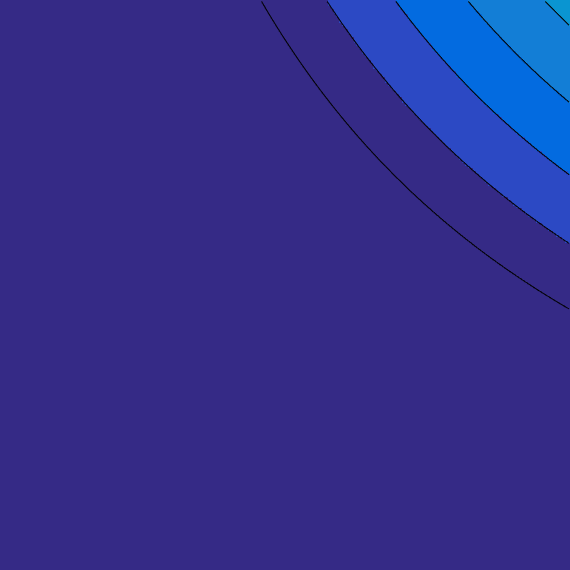
\includegraphics[width=.19\linewidth]{soft-min/lse-1}&
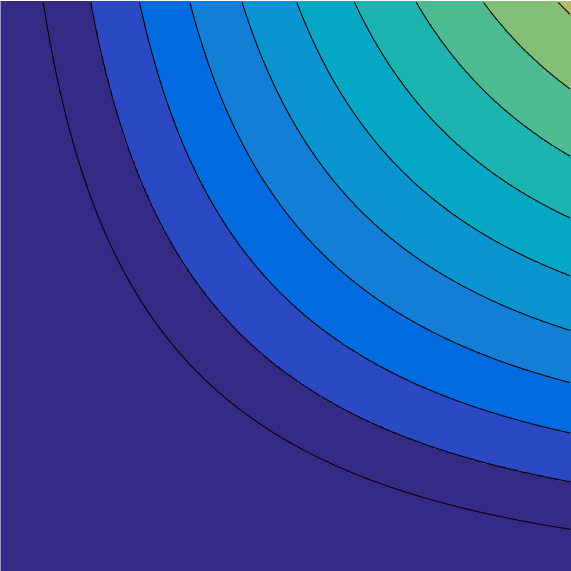
\includegraphics[width=.19\linewidth]{soft-min/lse-05}&
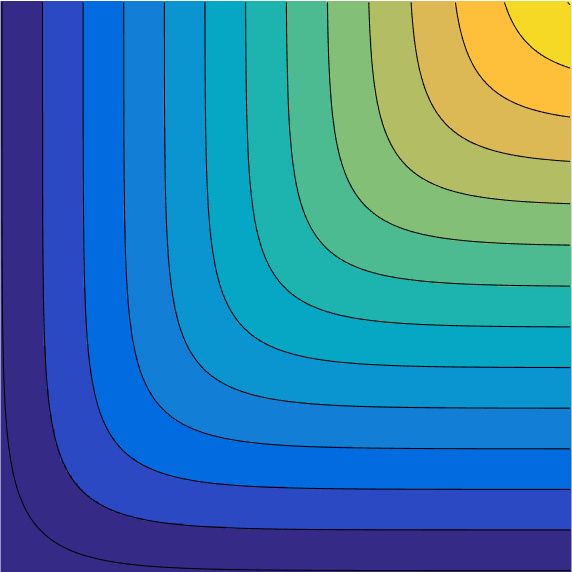
\includegraphics[width=.19\linewidth]{soft-min/lse-01}&
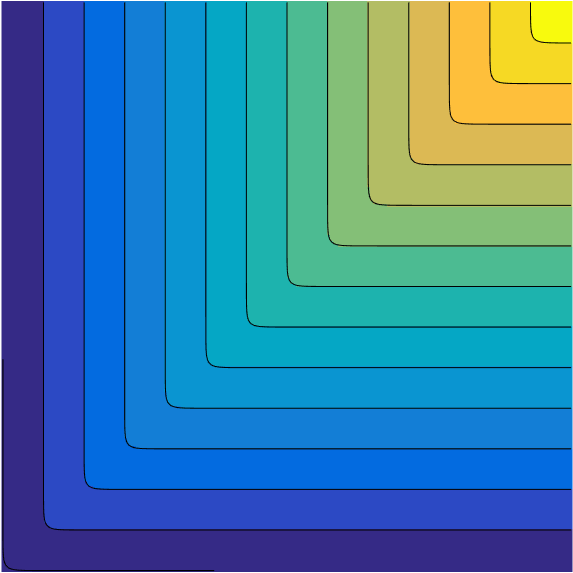
\includegraphics[width=.19\linewidth]{soft-min/lse-001}&
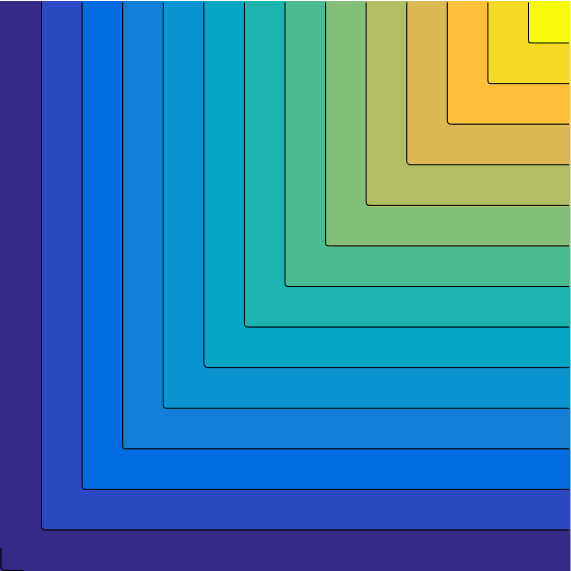
\includegraphics[width=.19\linewidth]{soft-min/lse-0001} \\
$\varepsilon=1$ &
$\varepsilon=0.5$ &
$\varepsilon=10^{-1}$ &
$\varepsilon=10^{-2}$ &
$\varepsilon=10^{-3}$
\end{tabular}
\caption{\label{fig-softmin}
2次元における関数$\smine(\z)$の表示、$\z \in \RR^2$、様々な$\varepsilon$に対して。
}
\end{figure}

この表記法を用いると、式~\eqref{eq-slse-sinkh-1}と~\eqref{eq-slse-sinkh-2}は次のように書き換えられる
\begin{align}
\label{eq-slse-smin-1}(\itt{\fD})_i &= \smine\, (\C_{ij}-\it{\gD}_j)_j + \varepsilon \log \a_i, \\
\label{eq-slse-smin-2}(\itt{\gD})_j &= \smine\, (\C_{ij}-\it{\fD}_i)_i + \varepsilon \log \b_j.
\end{align}
ここで$\smine\, (\C_{ij}-\it{\gD}_j)_j$は行列$(\C-\ones_n (\it{\gD})^\top )$の$j$列のすべての値のソフト最小値を表す。表記を簡略化するために、行列を入力として取り、その列または行のソフト最小値の列ベクトルを出力する演算子を導入する。すなわち、任意の行列$A\in\RR^{n\times m}$に対して
\begin{align*}
	\SMINEr(\A) \eqdef \pa{\smine \pa{\A_{i,j}}_j}_i\in\RR^n,\\
	\SMINEc(\A) \eqdef \pa{\smine \pa{\A_{i,j}}_i}_j\in\RR^m.
\end{align*}
と定義する。これらの演算は\S\ref{sec-semi-discr-entropy}で導入されるエントロピー的$\c$-変換と等価であることに注意する（特に~\eqref{eq-sinkh-c-transf}を参照）。
%
この表記法を用いると、Sinkhornの反復は次のように書ける
\begin{align}
	\label{eq-lse-dual-1}\itt{\fD} &= \SMINEr\, (\C-\ones_n\transp{\it{\gD}}) + \varepsilon \log \a, \\
	\label{eq-lse-dual-2}\itt{\gD} &= \SMINEc\, (\C-\it{\fD}\transp{\ones_m})  + \varepsilon \log \b.
\end{align}
$\varepsilon \rightarrow 0$のとき$\smine$は$\min$に収束するが、$\varepsilon=0$の極限では反復はもはや収束しない。なぜなら交互最小化は制約付き問題では収束せず、これは非正則化双対~\eqref{eq-dual}の場合だからである。
\end{rem}
%%%%%%%%%%



%%%%%%%%%%
\begin{rem}[対数領域Sinkhorn]\label{rem-log-sinkh}
Sinkhorn更新~\eqref{eq-sinkhorn}と数学的に等価であるが、反復~\eqref{eq-slse-smin-1}と~\eqref{eq-slse-smin-2}は、小さな$\varepsilon$の値に対するアンダーフローを回避するために\emph{ログサムエクスポネンシャル}安定化トリックの使用を示唆する。$\underbar{z}=\min \z$と書くと、そのトリックは$\smine \z$を次のように評価することを示唆する
\eql{\label{eq-log-domain-min}
	\smine \z = \underbar{z} -\varepsilon \log \sum_i e^{-(\z_i-\underbar{z})/\varepsilon}.
}
~\eqref{eq-log-domain-min}のように$\underbar{z}$を引いて対数領域反復を安定化する代わりに、実際には以前に計算されたスケーリングを引くことができる。
これは安定化された反復につながる
\begin{align}
	\label{eq-lse-sinkh-1}\itt{\fD} &= \SMINEr( \logP(\it{\fD},\it{\gD}))  + \it{\fD} + \varepsilon\log(\a), \\
	\label{eq-lse-sinkh-2}\itt{\gD} &= \SMINEc( \logP(\itt{\fD},\it{\gD})) + \it{\gD} + \varepsilon \log(\b),
\end{align}
ここで
\eq{
	\logP(\fD,\gD) = \pa{\C_{i,j} - \fD_i - \gD_j}_{i,j}.
}
と定義した。
% The log-sum-exp operators are defined as
% \begin{align*}
% 	\foralls i \in \range{n}, \quad \LSE_1(\logP)_i &= \varepsilon \log \sum_j \exp( \logP_{i,j} ), \\
% 	\foralls j \in \range{m}, \quad \LSE_2(\logP)_j &= \varepsilon \log \sum_i \exp( \logP_{i,j} ).
% \end{align*}
もとの反復~\eqref{eq-sinkhorn}とは対照的に、これらの対数領域反復~\eqref{eq-lse-sinkh-1}と~\eqref{eq-lse-sinkh-2}は任意の$\varepsilon>0$に対して安定である。
なぜなら量$\logP(\fD,\gD)$は反復中に有界に留まるからである。
欠点は、各ステップで$nm$回の$\exp$の計算が必要なことである。
$\SMINEr$または$\SMINEc$の計算は、行列積よりも通常大幅に遅く、行列$\logP$の行ごとのソフト最小値の計算を必要とする。したがって、複数の周辺分布に対するSinkhorn写像の適用を効率的に並列化する方法は存在しない。
%
小さな次元のEuclid領域では、計算を大幅に高速化するために、減衰する$\varepsilon$戦略とスパースグリッドを用いた効率的なマルチスケール解法を開発することが可能である~\citep{schmitzer2016stabilized}。
\end{rem}
%%%%%%%%%%




%%%%%%%%%%
\begin{rem2}{一般的な測度に対する双対}
一般的な（必ずしも離散でない）入力測度$(\al,\be)$に対して、双対問題~\eqref{eq-dual-formulation}は次のようになる
\eql{\label{eq-dual-entropic}
	\usup{(\f,\g) \in \Cc(\X)\times\Cc(\Y)} \int_\X \f \d\al + \int_\Y \g \d\be
		 - \varepsilon \int_{\X\times\Y} e^{ \frac{-c(x,y)+f(x)+g(y)}{\varepsilon} } \d\al(x)\d\be(y).
}
これはもとの問題~\eqref{eq-dual-generic}に現れる制約$\Potentials(\c)$の平滑化に対応し、$\varepsilon \rightarrow 0$の極限で復元される。
%
エントロピー輸送の場合にこれらのカントロビッチポテンシャル$(\f,\g)$の存在（すなわち上限が実際に最大値であること）を証明することは、古典的なOTの場合より容易ではない。なぜなら$c$-変換を使うことができず、ポテンシャルは自動的にLipschitzにならないからである。存在の証明はSinkhorn反復の収束を用いて行うことができる；詳細は~\citep{2016-chizat-sinkhorn}を参照。
\end{rem2}
%%%%%%%%%%




%%%%%%%
\begin{rem2}{制約なしエントロピー双対}
注意~\ref{rem-uncons-dual}と同様に、$\int_\X \d\mu=\int_\Y\d\nu = 1$の場合、代替的な双対定式化を考えることができる
\eql{\label{eq-dual-entropic-alt}
	\usup{(\f,\g) \in \Cc(\X)\times\Cc(\Y)} \int_\X \f \d\al + \int_\Y \g \d\be
		+ \smine( c - f \oplus g ),
}
これは~\eqref{eq-dual-entropic}と同じ最適値を達成する。
%
~\eqref{eq-defn-softmin}と同様に、ソフト最小値（ここでは$\X \times \Y$上）は次のように定義される
\eq{
	\foralls S \in \Cc(\X\times\Y), \quad
	\smine S \eqdef
	- \varepsilon \int_{\X\times\Y} e^{ \frac{-S(x,y)}{\varepsilon} } \d\al(x)\d\be(y)
}
（これは$(\al,\be)$に依存することに注意する）。
%
$\epsilon \rightarrow 0$のとき、$\smine \rightarrow \min$であり、非正則化かつ制約なし定式化~\eqref{eq-dual-uncons}で使われるものに帰着する。
%
~\eqref{eq-dual-entropic}と~\eqref{eq-dual-entropic-alt}はともに制約なし問題であるが、
~\eqref{eq-dual-entropic-alt}の主な利点は条件が良いことである。
汎関数のHesse行列が$\epsilon$で一様に有界であるという意味においてである。
このような条件数の改善を得るもう1つの方法は半双対問題を考えることである；
\S\ref{sec-semi-discr-entropy}、特に注意~\ref{rem-second-order-smoothness}を参照。
%
この代替的な双対定式化の欠点は、対数の存在により\S\ref{sec-sgd}で詳述される確率的最適化手法の使用が妨げられることである；特に注意~\ref{rem-sgd-cont-cont}を参照。
\end{rem2}
%%%%%%%

%%%%%%%%%%%%%%%%%%%%%%%%%%%%%%%%%%%%%%%%%%%%%%%%%%%%%%%%%%%%%%%%%%%%%%%%%%
\section{最適輸送コストの正則化近似}
\label{sec-regularized-cost}

エントロピー双対~\eqref{eq-dual-formulation}は滑らかな制約なし凹最大化問題であり、以下の命題で詳述するように、もとのカントロビッチ双対~\eqref{eq-dual}を近似する。\todoK{explain soft indicator constraint, transition to result below.}

\begin{prop}\label{prop-feasibility-dual}
~\eqref{eq-dual-formulation}の最適解の任意のペア$(\fD^\star,\gD^\star)$は、$(\fD^\star,\gD^\star) \in \PotentialsD(\C)$（~\eqref{eq-feasible-potential}で定義された実行可能カントロビッチポテンシャルの集合）を満たす。結果として、任意の$\varepsilon$に対して
\eq{
	\dotp{\fD^\star}{\a} + \dotp{\gD^\star}{\b} \leq  \MKD_\C(\a,\b).
}
\end{prop}
\begin{proof}
	~\eqref{eq-prim-dual-ent}における主-双対最適性条件と、$\P$が確率分布であり従ってすべての$i,j$に対して$\P_{i,j}\leq 1$であるという制約から、$\exp(-(\fD^\star_i+\gD^\star_j-\C_{i,j})/\varepsilon)\leq 1$が得られ、したがって$\fD^\star_i+\gD^\star_j\leq\C_{i,j}$となる。
\end{proof}

~\eqref{eq-regularized-discr}で定義される正則化輸送コスト$\MKD_\C^\varepsilon$の主な利点は、それが滑らかで凸であることであり、変分問題における損失関数としての統合に最適である（第~\ref{c-variational}章を参照）。

\begin{prop}\label{prop-convexity-dual}
$\MKD_\C^\varepsilon(\a,\b)$は$\epsilon\geq 0$に対して$\a$と$\b$の同時凸関数である。$\epsilon>0$のとき、その勾配は次に等しい
\eq{
	\nabla\MKD_\C^\varepsilon(\a,\b)= \begin{bmatrix} \fD^\star \\ \gD^\star \end{bmatrix},
}
ここで$\fD^\star$と$\gD^\star$は、座標の和が0になるように選ばれた式~\eqref{eq-dual-formulation}の最適解である。
\end{prop}

\todoK{
\begin{proof}
	\todo{TODO}
\end{proof}
}


\citep{CuturiSinkhorn}において、2つのヒストグラム間のWasserstein距離を近似するための下界と上界が提案された。これらの界はSinkhornアルゴリズムによって得られる解において主問題と双対問題の目的関数を評価することから成る。

\begin{defn}[Sinkhorn・ダイバージェンス]
	$\fD^\star$と$\gD^\star$を~\eqref{eq-dual-formulation}の最適解、$\P^\star$を~\eqref{eq-regularized-discr}の解とする。Wasserstein距離は以下の主Sinkhorn・ダイバージェンスと双対Sinkhorn・ダイバージェンスを用いて近似される：
\begin{align*}
	\SINKHORNP_\C^\varepsilon(\a,\b)& \eqdef \dotp{\C}{\P^\star} =  \dotp{e^{\frac{\fD^\star}{\varepsilon}}}{(\K\odot \C)e^{\frac{\gD^\star}{\varepsilon}}}, \\
	\SINKHORND_\C^\varepsilon(\a,\b) & \eqdef \dotp{\fD^\star}{\a} + \dotp{\gD^\star}{\b},
\end{align*}
ここで$\odot$は行列の成分ごとの積を表す。
\end{defn}

\begin{prop}\label{prop-sinkhorn-div}
次の関係が成り立つ：
\eq{
	\SINKHORND_\C^\varepsilon(\a,\b)\leq \MKD_\C^\varepsilon(\a,\b) \leq \SINKHORNP_\C^\varepsilon(\a,\b).
}
さらに
\eql{\label{eq-sinkh-div-gap}
	\SINKHORNP_\C^\varepsilon(\a,\b) - \SINKHORND_\C^\varepsilon(\a,\b) = \varepsilon ( \HD(\P^\star)+1 ) .
}
\end{prop}
\begin{proof}
式~\eqref{eq-sinkh-div-gap}は、主問題と双対問題が最適値において同じ値を持つこと（~\eqref{eq-dual-formulation}を参照）から、
\eq{
	\MKD_\C^\varepsilon(\a,\b) = \SINKHORNP_\C^\varepsilon(\a,\b) - \varepsilon \HD(\P^\star) =
	\SINKHORND_\C^\varepsilon(\a,\b) - \varepsilon \dotp{e^{\fD^\star/\varepsilon} }{ \K e^{\gD^\star/\varepsilon}}
}
と書くことで得られる。最終結果は$\dotp{e^{\fD^\star/\varepsilon} }{ \K e^{\gD^\star/\varepsilon}}=1$であることに注意することで得られる。後者は$\P^\star$のすべての成分の和を計算することに相当するからである。
\end{proof}


上で与えた関係式はOT距離を実際に界で挟む実用的な方法を示唆するが、実際にはSinkhornアルゴリズムの収束時にのみ有効であり、したがって実際には真に有用ではない。実際には、Sinkhorn反復は常にある精度の閾値に達した後で終了される。所定の反復回数$L$が設定され、最適解$\fD^\star$と$\gD^\star$の代わりに反復$\itL{\fD}$と$\itL{\gD}$を用いて$\SINKHORND_\C^\varepsilon$を評価すると、下界が回復される：式~\eqref{eq-lse-sinkh-1}と~\eqref{eq-lse-sinkh-2}に現れる表記法を用いて、$\MKD_\C^\varepsilon$の次の有限ステップ近似を導入する：
\eql{\label{eq-algorithmic-loss}
	\itL{\SINKHORND_\C}(\a,\b) \eqdef \dotp{\itL{\fD}}{\a} + \dotp{\itL{\gD}}{\b}.
}
この「アルゴリズム的」Sinkhorn汎関数は$L\geq 1$の場合に正則化コスト関数の下界を与える。


\begin{prop}[有限Sinkhorn・ダイバージェンス]\label{defn-sinkhorn-div}
次の関係が成り立つ：
\eq{
	\itL{\SINKHORND_\C}(\a,\b) \leq \MKD_\C^\varepsilon(\a,\b).
}
\end{prop}
\begin{proof}命題~\ref{prop-feasibility-dual}の証明と同様に、たった1回のSinkhorn反復の後でも、~\eqref{eq-slse-sinkh-1}と~\eqref{eq-slse-sinkh-2}に従って、$\itL{\fD}$と$\itL{\gD}$は成分$\exp(-(\itL{\fD}_i+\itL{\gD}_j-\C_{i,j})/\varepsilon)$を持つ行列の列和が$\b$であり、したがってその各成分は1以下であるという事実を利用する。これにより$(\itL{\fD}_i,\itL{\gD})$の双対実行可能性が得られる。
\end{proof}

\begin{rem}[Sinkhorn反復の主問題における非実行可能性]
\eqref{eq-sink-matrix}で提供される主反復は主問題において実行可能ではないことに注意する。なぜなら定義上、これらの反復は収束時に周辺制約を満たすよう設計されているからである。したがって$\P^{(2L+1)}$は実行可能ではないため、$\dotp{\C}{\P^{(2L+1)}}$を$\MKD_\C(\a,\b)$の近似と見なすことは妥当ではない。注意~\ref{rem-complexity-rounding}で述べた~\citet{altschuler2017near}の丸めスキームを用いることで、$\MKD_\C^\varepsilon(\a,\b)$の上界を得ることができる。さらに、Sinkhornアルゴリズムと同様に~\citep{NIPS2018_8184}、複数のヒストグラムのペアに対して行列演算を用いて並列に便利に計算できる。
\end{rem}


\begin{rem}[有限双対Sinkhorn・ダイバージェンスの非凸性] ~\eqref{eq-dual-formulation}の正則化された式$\MKD_\C^\varepsilon$とは異なり、有限Sinkhorn・ダイバージェンス$\itL{\SINKHORND_\C}(\a,\b)$は一般にその引数の凸関数\emph{ではない}（数値的に容易に確認できる）。しかし$\itL{\SINKHORND_\C}(\a,\b)$は微分可能な関数であり、自動微分技法を用いて（注意~\ref{rem-auto-diff}を参照）任意の引数、特に$\C,\a$または$\b$に関して微分できる。
\end{rem}
\todoK{ automatically differentiated using the following recursion:\todo{write recursion}.}




%%%%%%%%%%%%%%%%%%%%%%%%%%%%%%%%%%%%%%%%%%%
\section{一般化Sinkhorn}
\label{sec-generalized}

正則化OT問題~\eqref{eq-regularized-discr}は、次の形の構造化凸最適化問題の特殊ケースである
\eql{\label{eq-generalized-ot-regul}
	\umin{\P}
		\sum_{i,j} \C_{i,j} \P_{i,j} - \varepsilon \HD(\P) + F( \P\ones_m ) + G( \transp{\P}\ones_n ).
}
実際、$F=\iota_{\{\a\}}$、$G=\iota_{\{\b\}}$と定義すると、閉凸集合$\Cc$の指示関数は
\eql{\label{eq-iota-function}
	\iota_{\Cc}(x) = \choice{
		0 \qifq x \in \Cc, \\
		+\infty \quad\text{otherwise},
	}
}
であり、$\Couplings(\a,\b)$を定義するハード周辺制約が復元される。
%
命題~\ref{prop-regularized-primal}の証明はこのより一般的な問題~\eqref{eq-generalized-ot-regul}にも適用されるため、~\eqref{eq-generalized-ot-regul}の一意の解も~\eqref{eq-scaling-form}の形を持つ。

~\citep{2015-Peyre-siims,FrognerNIPS,2016-chizat-sinkhorn,karlsson2016generalized}で示されたように、Sinkhorn反復~\eqref{eq-sinkhorn}はこの問題に拡張でき、次のように書ける
\eql{\label{eq-gen-sinkh}
	\uD \leftarrow \frac{\Prox_{F}^{\KLD}(\K \vD)}{\K \vD}
	\qandq
	\vD \leftarrow \frac{\Prox_{G}^{\KLD}(\transp{\K}\uD)}{\transp{\K}\uD},
}
ここで$\KLD$ダイバージェンスに対する近接作用素は
\eql{\label{eq-prox-kl}
	\foralls \uD \in \RR_+^N, \quad
	\Prox_{F}^{\KLD}(\uD) = \uargmin{\uD' \in \RR_+^N}	\KLD(\uD'|\uD) + F(\uD').
}
一部の関数$F,G$に対しては反復~\eqref{eq-gen-sinkh}の線形収束率を証明することが可能であり、これらのスキームは任意の測度に一般化できる；詳細は~\citep{2016-chizat-sinkhorn}を参照。

反復~\eqref{eq-gen-sinkh}は、$\Prox_{F}^{\KLD}$と$\Prox_{G}^{\KLD}$が閉じた形で、または非常に効率的に計算できる場合に興味深い。これは特に$F(\uD) = \sum_i F_i(\uD_i)$の形の分離可能関数の場合であり、このとき
\eq{
	\Prox_{F}^{\KLD}(\uD) = \pa{ \Prox_{F_i}^{\KLD}(\uD_i) }_i.
}
各$\Prox_{F_i}^{\KLD}$の計算は、スカラー最適化問題であるため通常単純である。
%
初期のSinkhornアルゴリズムと同様に、対数領域での計算を用いて計算を安定化することも可能であることに注意する~\citep{2016-chizat-sinkhorn}。

このアルゴリズムはOTの様々な一般化の解を近似するために使用でき、特に~\eqref{eq-unbalanced-pbm}の形の非均衡OT問題（\S\ref{sec-unbalanced}、特に反復~\eqref{eq-iterate-gen-sinkh}を参照）および~\eqref{eq-grad-flow-discr}の形の勾配流問題（\S\ref{sec-grad-flows}を参照）に使用できる。


%%%
\begin{rem1}{双対性とLegendre変換}
~\eqref{eq-generalized-ot-regul}の双対問題は次のようになる
\eql{\label{eq-dual-generalized}
	\umax{\fD,\gD}
		- F^*( \fD ) -G^*(\gD)
		- \varepsilon\sum_{i,j} e^{ \frac{\fD_i+\gD_j-\C_{i,j}}{\varepsilon} }
}
したがって$(\uD,\vD) = (e^{\fD/\varepsilon},e^{\gD/\varepsilon})$が~\eqref{eq-scaling-form}に現れる対応するスケーリングである。
ここで$F^*$と$G^*$はFenchel-Legendre共役であり、次のように定義される凸関数である
\eql{\label{eq-legendre}
		\foralls \fD \in \RR^n, \quad
		F^*(\fD) \eqdef \umax{\a \in \RR^n} \dotp{\fD}{\a} - F(\a).
}
%
一般化Sinkhorn反復~\eqref{eq-gen-sinkh}はDykstraアルゴリズム~\citep{Dykstra83,Dykstra85}（Bregman・ダイバージェンスに拡張されたもの~\citep{bauschke-lewis,CensorReich-Dykstra}；注意~\ref{rem-bregman}も参照）の特殊ケースであり、双対問題~\eqref{eq-dual-generalized}に対する交互最大化スキームである。
\end{rem1}
%%%

定式化~\eqref{eq-generalized-ot-regul}は2つ以上の関数および単一のカップリングを超えてさらに一般化できる；詳細は~\citep{2016-chizat-sinkhorn}を参照。これには特殊ケースとして、\S\ref{sec-multimarginal}で詳述する多周辺問題に対するSinkhornアルゴリズム~\eqref{eq-sinkh-multimarg}が含まれる。
%
正則化重心問題~\eqref{eq-entropic-bary}をこのように書き換えることも可能であり、反復~\eqref{eq-sinkhorn-bary}は実際にこの一般化Sinkhornの特殊ケースである。


\if 0 %% REMOVED %%%
\eq{
	\umin{(\P_s)_{s=1}^S}
		\sum_{i,j,s} \C_{s,i,j} \P_{s,i,j} - \varepsilon \HD(\P_s) +
		\sum_{k} F_k( (\P_s\ones_m)_s, (\transp{\P_s}\ones_n)_s )
}
where $\{\C_s\}_s$ are given cost matrices.

The solution has the form
\eql{\label{eq-scaling-form-multi}
	\foralls (s,i,j) \in \range{1,S} \times \range{n} \times \range{m}, \quad
	\P_{s,i,j} =  \K_{s,i,j} \prod_{k} \uD_{k,i} \prod_\ell \vD_{k,j}
}
where $\K_s=e^{-\C_s/\varepsilon}$ is a Gibbs kernel, and $(\uD_k,\vD_\ell)_{k,\ell}$ are scaling vectors that need to be computed using Generalized Sinkhorn iterations similar to~\eqref{eq-gen-sinkh}~\citep{2016-chizat-sinkhorn}.
%
In the case where the functions $F_s$ are indicator functions, one retrieves the Sinkhorn algorithm~\eqref{eq-sinkh-multimarg} for the multi-marginal problem, as detailed in~\S\ref{sec-multimarginal}.
%
It is also possible to rewrite the regularized barycenter problem~\eqref{eq-entropic-bary} this way, and the iterations~\eqref{eq-sinkhorn-bary} are in fact a special case of this generalized Sinkhorn.

\fi %%%%

\todoK{Write down the generalized iterations}

%These iterations read
%\eq{
%	\foralls k, \quad
%	\uD_s \leftarrow \frac{\Prox_{F_k}^{\KLD}( \tilde \uD_k \K \vD }{ \tilde \uD_k }
%	\qwhereq
%	\prod \uD_ \K \vD
%}
%\eq{
%	\vD \leftarrow \frac{\Prox_{G}^{\KLD}(\transp{\K}\uD)}{\transp{\K}\uD}.
%}
%where we defined the Gibbs kernel associated to the cost matrix $\C$ as
%\eq{
%	\K_{i,j} \eqdef e^{-\frac{\C_{i,j}}{\varepsilon}}
%}

% !TEX root = ../ComputationalOTFnT.tex

\chapter{半離散最適輸送}
\label{c-algo-semidiscr}

本章では、二つの入力測度の一方が離散（Dirac質量の和）であり、もう一方が任意の測度である場合、特にLebesgue測度に関して密度を持つ場合の最適輸送問題に取り組む手法を研究する。
%
周囲空間の次元が低い場合、この問題は強い幾何学的性質を持つ。なぜなら、連続密度から離散測度への最適輸送は区分的に定数な写像であり、離散測度の台の各点の逆像は互いに素なセルの和集合となることが示されるからである。
%
コストがEuclid距離の二乗である場合、これらのセルは計算幾何学における重要な概念であるいわゆるLaguerreセルに対応する。Laguerreセルとは、定数だけオフセットされたVoronoiセルである。この関係により、計算幾何学のツールを借用して高速な計算スキームを得ることが可能となる。
%
高次元においては、半離散定式化は確率的計画問題としても解釈でき、わずかな正則化の恩恵を受けることもできる。これにより、第~\ref{c-entropic}~章で提示したエントロピー正則化スキームの応用範囲が拡張される。
%
これらの構成はすべて$c$-変換の概念に大きく依存しており、ここでは\S\ref{sec-c-transforms}のように行列に限らず、一般的なコスト関数に対するものである。$c$-変換は凸解析におけるLegendre変換の一般化であり、最適輸送の理論およびアルゴリズムにおいて中心的な役割を果たす。

%%%%%%%%%%%%%%%%%%%%%%%%%%%%%%%%%%%%%%%%%%%%
\section{$c$-変換と$\bar c$-変換}
\label{s-c-transform}

双対最適輸送問題~\eqref{eq-dual-generic}は以下のように書けることを思い出そう。
\eq{
	\usup{(\f,\g)}
			\Ee(\f,\g) \eqdef
			\int_\X \f(x) \d\al(x) + \int_\Y \g(y) \d\be(y) + \iota_{\Potentials(\c)}(\f,\g),
}
ここで有用な指示関数の記法~\eqref{eq-iota-function}を用いた。双対ポテンシャル$\f$または$\g$のいずれかを固定し、それぞれ$\g$または$\f$に関して最適化すると、$\c$-変換の定義を与える閉じた形の解が得られる：
\begin{align}\label{eq-c-transform}
	\foralls y \in \Y, \quad
	\f^\c(y) &\eqdef \uinf{x \in \X} \c(x,y) - \f(x), \\
	\foralls x \in \X, \quad
	\g^{\bar\c}(x) &\eqdef \uinf{y \in \Y} \c(x,y) - \g(y),
\end{align}
ここで$\bar\c(y,x) \eqdef c(x,y)$と記した。
%
実際、以下が成り立つことを確認できる。
\eql{\label{eq-alternate-c-transf}
	\f^\c \in \uargmax{\g} \Ee(\f,\g)
	\qandq
	\g^{\bar\c} \in \uargmax{\f} \Ee(\f,\g).
}
これらの部分最小化は、それぞれ$\al$と$\be$の台上で最大化元を定義するが、定義~\eqref{eq-c-transform}は実際には空間$\X$と$\Y$全体上の関数を定義することに注意されたい。これは、~\eqref{eq-dual-generic}の解を空間全体に標準的に拡張する方法である。
%
$\X=\RR^d$かつ$c(x,y)=\norm{x-y}_2^p=(\sum_{i=1}^d \abs{x_i-y_i})^{p/2}$のとき、$\c$-変換~\eqref{eq-c-transform}の$\f^\c$は$-\f$と$\norm{\cdot}^p$のいわゆる下限畳み込みである。$\f^\c$の定義は「ホップ・ラックスの公式」とも呼ばれる。

写像$(\f,\g) \in \Cc(\X) \times \Cc(\Y) \mapsto (\g^{\bar\c},\f^\c) \in \Cc(\X) \times \Cc(\Y)$は、双対ポテンシャルを「より良い」もの（双対目的関数$\Ee$を改善する）に置き換える。$\f^\c$および$\g^{\bar\c}$の形に書ける関数は、$c$-凹関数および$\bar c$-凹関数と呼ばれる。
%
$\X=\Y=\RR^\dim$において$\c(x,y)=\dotp{x}{y}$という特別な場合には、この定義は通常の凹関数の概念と一致する。
%
命題~\ref{prop-ccc-2}を連続の場合に自然に拡張すると、以下の性質が成り立つ。
\eq{
	\f^{c\bar c c} = \f^c
	\qandq
	\g^{\bar c c \bar c} = \g^{\bar c},
}
ここで$\f^{c\bar c} = (\f^{c})^{\bar c}$と記した。この不変性は、この方法で双対ポテンシャルを「改善」できるのは一度だけであることを示している。別の言い方をすれば、交互最大化は収束しない（直ちにサイクルに入る）ということであり、これは最適化変数の非滑らかな（制約による）結合を含む汎関数の古典的な性質である。これは第~\ref{c-entropic}~章で示される最適輸送のエントロピー正則化とは対照的である。エントロピー正則化の場合、正則化により双対目的関数~\eqref{eq-dual-formulation}は滑らかであり、交互最大化はSinkhorn反復~\eqref{eq-lse-sinkh-1}および~\eqref{eq-lse-sinkh-2}に対応する。これらの反復は、双対変数上で記述すると、$c$-変換のエントロピー的に平滑化されたバージョンを定義し、$\min$演算が「ソフト最小」に置き換えられる。

~\eqref{eq-alternate-c-transf}を用いて、~\eqref{eq-dual-generic}を単一のポテンシャルに関する制約なし凸計画問題として再定式化できる。
\begin{align}\label{eq-semi-dual-cont}
	\MK_\c(\al,\be)
		&= \usup{\f \in \Cc(\X)}
			\int_\X \f(x) \d\al(x) + \int_\Y \f^{c}(y) \d\be(y) \\
		&= \usup{\g \in \Cc(\Y)}
			\int_\X \g^{\bar\c}(x) \d\al(x) + \int_\Y \g(y) \d\be(y).
\end{align}
写像$(\f,\g) \mapsto (\g^{\bar\c},\f^\c)$を反復適用できるため、$\f$が$\bar c$-凹であり$\g$が$\c$-凹であるという制約を追加することが可能であり、これはポテンシャルの十分な正則性を確保し、例えば~\eqref{eq-dual-generic}の解の存在を示すために重要である。

%%%%%%%%%%%%%%%%%%%%%%%%%%%%%%%%%%%%%%%%%%%%
\section{半離散定式化}
\label{s-semidiscrete}

特に興味深い場合は、$\be = \sum_j \b_j \de_{y_j}$が離散である場合である（もちろん$\al$が離散の場合にも、$\al$と$\be$の役割を入れ替えることで同じ構成が適用される）。
%
$\bar c$変換~\eqref{eq-c-transform}の定義を、$\be$の台$(y_j)_j$に最小化を制限することでこの設定に適応できる。
\eql{\label{eq-disc-c-transfo}
	\foralls \gD \in \RR^m, \;
	\foralls x \in \Xx, \quad
	\gD^{\bar \c}(x) \eqdef \umin{j \in \range{m}} \c(x,y_j) - \gD_j.
}
この変換はベクトル$\gD$を連続関数$\gD^{\bar \c} \in \Cc(\Xx)$に写す。
%
この定義は、空間$\X$が$\be$の台に等しいと課した場合の~\eqref{eq-c-transform}と一致することに注意されたい。
%
図~\ref{fig-c-transform-discrete}に、1次元および2次元におけるこのような離散$\bar c$-変換の例を示す。


\newcommand{\MyFigCTrans}[1]{\includegraphics[width=.24\linewidth,trim=63 40 48 30,clip]{c-transform-2d/c-transform-p#1}}
\begin{figure}[h!]
\centering
%%% 1D %%%

\includegraphics[width=.8\linewidth]{c-transform-1d/c-transform-p.pdf}\vspace{2mm}
%%% 2D %%%
\begin{tabular}{@{}c@{\hspace{1mm}}c@{\hspace{1mm}}c@{\hspace{1mm}}c@{}}
\MyFigCTrans{5}&
\MyFigCTrans{10}&
\MyFigCTrans{15}&
\MyFigCTrans{20}\\
$p=1/2$ & $p=1$ & $p=3/2$ & $p=2$
\end{tabular}
\caption{\label{fig-c-transform-discrete}
上段：1次元における半離散$\bar c$-変換$\gD^{\bar \c}$の例。基底コスト$c(x,y)=|x-y|^p$に対して$p$を変化させたもの（カラーバー参照）。
%
赤い点は位置$(y_j,-\gD_j)_j$にある。
%
下段：2次元における半離散$\bar c$-変換$\gD^{\bar \c}$の例。基底コスト$c(x,y)=\norm{x-y}_2^p=(\sum_{i=1}^d \abs{x_i-y_i})^{p/2}$に対して$p$を変化させたもの。
%
赤い点は位置$y_j \in \RR^2$にあり、その大きさは$\gD_j$に比例する。
%
太い黒い曲線で区切られた領域は、これらの点$(y_j)_j$に関連するLaguerreセル$(\Laguerre_{j}(\gD))_j$である。
}
\end{figure}

重要なことに、半離散問題~\eqref{eq-semi-dual-cont}において離散$\bar c$-変換を用いると、有限次元の最適化問題が得られる。
\eql{\label{eq-semi-dual-discr}
	\MK_\c(\al,\be) =
		\umax{\gD \in \RR^m}
			\Ee(\gD) \eqdef
			\int_\X \gD^{\bar \c}(x) \d\al(x) + \sum \gD_y \b_j.
}

双対重み$\gD$に関連するLaguerreセル
\eq{
	\Laguerre_{j}(\gD) \eqdef \enscond{x \in \X}{ \foralls j' \neq j, \c(x,y_j) - \gD_j \leq \c(x,y_{j'}) - \gD_{j'} }
}
は$\X = \bigcup_j \Laguerre_{j}(\gD)$の互いに素な分解を誘導する。$\gD$が定数のとき、Laguerreセル分解は空間のVoronoi図分割に対応する。
%
図~\ref{fig-c-transform-discrete}の下段は、2次元におけるLaguerreセルの分割の例を示している。

これにより、最小化されるエネルギーを以下のように便利に書き直すことができる。
\eql{\label{eq-semi-disc-energy}
	\Ee(\gD) = \sum_{j=1}^m \int_{\Laguerre_{j}(\gD)} \pa{ c(x,y_j) - \gD_j } \d\al(x) + \dotp{\gD}{\b}.
}
この関数の勾配は以下のように計算できる：
\eq{
	\foralls j \in \range{m}, \quad
	\nabla\Ee(\gD)_j = - \int_{\Laguerre_{j}(\gD)} \d\al(x) + \b_j.
}
図~\ref{fig-semi-discr}は、$\Ee$を最小化するための勾配降下法の反復を表示している。
%
最適な$\gD$が計算されると、$\al$から$\be$への最適輸送写像$\T$は、任意の$x \in \Laguerre_{j}(\gD)$を$y_j$に写す区分的に定数な写像となる。

$\c(x,y)=\norm{x-y}^2$という特別な場合、Laguerreセルへの分解は「パワーダイアグラム」とも呼ばれる。
%
セルは多面体であり、計算幾何学のアルゴリズムを用いて効率的に計算できる。\citep{aurenhammer1987power}を参照されたい。
%
最も広く用いられているアルゴリズムは、$\RR^\dim$における点のパワーダイアグラムが、点の集合$( (y_j,\norm{y_j}^2 - \gD_j) )_{j=1}^m \subset \RR^{\dim+1}$の凸包の$\RR^\dim$への射影に等しいという事実に基づいている。凸包を計算するアルゴリズムは多数存在する。例えば、\citet{chan1996optimal}の2次元および3次元におけるアルゴリズムは計算量$O(m\log(Q))$であり、ここで$Q$は凸包の頂点数である。
%
\todoK{Maybe make a drawing of this projection.}

%\newcommand{\MyFigSemiD}[1]{\includegraphics[width=.19\linewidth]{semi-discrete/#1}}
%\begin{figure}[h!]
%\centering
%\begin{tabular}{@{}c@{\hspace{1mm}}c@{\hspace{1mm}}c@{\hspace{1mm}}c@{\hspace{1mm}}c@{}}
%\MyFigSemiD{iteration-1} &
%\MyFigSemiD{iteration-3} &
%%\MyFigSemiD{iteration-8} &
%\MyFigSemiD{iteration-9} &
%\MyFigSemiD{iteration-13} &
%\MyFigSemiD{matching} \\
%$\ell=1$ &
%$\ell=3$ &
%$\ell=50$ &
%$\ell=100$ &
%Matching
%\end{tabular}
%\caption{\label{fig-semi-discr}
%Iterations of the semi-discrete OT algorithm minimizing~\eqref{eq-semi-disc-energy} (here a simple gradient descent is used).
%%
%The support $(y_j)_j$ of the discrete measure $\be$ is indicated by the red points, while the continuous measure $\al$ is the uniform measure on a square.
%%
%The blue cells display the Laguerre partition $( \Laguerre_{j}( \it{\gD} ) )_j$ where $\it{\gD}$ is the discrete dual potential computed at iteration $\ell$.
%}
%\end{figure}

\newcommand{\MyFigSemiD}[1]{\includegraphics[width=.19\linewidth]{semidiscrete-gd/#1}}
\begin{figure}[h!]
\centering
\begin{tabular}{@{}c@{\hspace{1mm}}c@{\hspace{1mm}}c@{\hspace{1mm}}c@{\hspace{1mm}}c@{}}
\MyFigSemiD{inputs} &
\MyFigSemiD{001} &
\MyFigSemiD{020} &
\MyFigSemiD{040} &
\MyFigSemiD{100}   \\
$\al$と$\be$ &
$\ell=1$ &
$\ell=20$ &
$\ell=40$ &
$\ell=100$
\end{tabular}
\caption{\label{fig-semi-discr}
~\eqref{eq-semi-disc-energy}を最小化する半離散最適輸送アルゴリズムの反復（ここでは単純な勾配降下法を使用）。
%
離散測度$\be$の台$(y_j)_j$は色付きの点で示され、連続測度$\al$は正方形上の一様測度である。
%
色付きのセルは、反復$\ell$で計算された離散双対ポテンシャル$\it{\gD}$に対応するLaguerre分割$( \Laguerre_{j}( \it{\gD} ) )_j$を表示している。
}
\end{figure}


Monge-Ampère方程式に対する半離散ソルバーの最初のアイデアは\citet{oliker1989numerical}によって提案され、双対変分問題との関係は\citet{AurenhammerHA98}によって示された。
%
理論的な解析と光学における反射板問題への応用は\citep{caffarelli1999problem}に詳述されている。
%
半離散定式化は\citep{carlier2010knothe}において、クノーテの輸送に基づく連続的アプローチと組み合わせて用いられた。
%
この手法が様々な分野で最近復活したのは、準Newtonソルバーを提案し計算幾何学の概念との関連を明確にした\citet{Merigot11}に負うところが大きい。最近の概観については\citep{Levy2017review}を参照されたい。コンピュータグラフィックスにおけるサンプリングに適用されるNewtonソルバーの使用は\citep{de2012blue}で提案されており、3次元の体積および表面処理への応用については\citep{levy2015numerical}も参照されたい。
%
半離散法の重要な応用分野は、Lagrange法を用いた非圧縮流体力学（Euler方程式）の解法である~\citep{deGoes2015,gallouet2017lagrangian}。半離散最適輸送ソルバーは、（重み付きの可能性がある）点群が領域内の一様分布を近似するよう課すことで、各反復において非圧縮性を強制する。
%
減衰Newton反復の（線形収束率での）収束は、Monge-Ampère方程式について\citep{mirebeau2015discretization}で証明され、最適輸送について\citep{kitagawa2016newton}で改良された。半離散最適輸送は照明設計、特に反射板の設計に重要な応用がある。\citep{merigot2017light}を参照されたい。

%%%%%%%%%%%%%%%%%%%%%%%%%%%%%%%%%%%%%%%%%%%%
\section{エントロピー半離散定式化}
\label{sec-semi-discr-entropy}

任意の測度間のエントロピー正則化問題~\eqref{eq-entropic-generic}の双対は、滑らかな制約なし最適化問題である：
\begin{equation}\label{eq-dual-entropic-generic}
	\MK_\c^\epsilon(\al,\be) =
	\usup{(\f,\g) \in \Cc(\X) \times \Cc(\Y)}
		 \int_\X \f\d\al + \int_\Y \g\d\be
		- \epsilon \int_{\X \times \Y}  e^{ \frac{-c + \f \oplus \g }{\epsilon} } \d\al\d\be,
\end{equation}
ここで$(f\oplus g)(x,y) \eqdef f(x)+g(y)$と記した。

非正則化問題~\eqref{eq-c-transform}と同様に、~\eqref{eq-dual-entropic-generic}において$\f$または$\g$のいずれかに関して明示的に最小化することができ、これにより平滑化された$\c$-変換が得られる。
\begin{align*}
	\foralls y \in \Y, \quad
	\f^{\c,\epsilon}(y) &\eqdef - \epsilon \log\pa{
			\int_{\X} e^{\frac{-\c(x,y) + \f(x)}{\epsilon}} \d\al(x)
	},\\
	\foralls x \in \X, \quad
	\g^{\bar\c,\epsilon}(x) &\eqdef - \epsilon \log\pa{
			\int_{\Y} e^{\frac{-\c(x,y) + \g(y)}{\epsilon}} \d\be(y)
	}.
\end{align*}
離散測度$\be = \sum_{j=1}^m \b_j\de_{y_j}$の場合、~\eqref{eq-semi-dual-discr}と同様に問題は簡略化され、離散双対ポテンシャル$\gD \in \RR^m$の関数として表される有限次元問題となる。
\eql{\label{eq-entropic-smoothed-c}
	\foralls x \in \X, \quad
	\gD^{\bar\c,\epsilon}(x) \eqdef - \epsilon \log\pa{
		\sum_{j=1}^m e^{\frac{-\c(x,y_j) + \gD_j}{\epsilon}} \b_j
	}.
}
離散測度$\al$の場合も同様に$\fD^{\bar\c,\epsilon}$を定義する。
%
ソフト最小演算子$\smine$を用いたSinkhornの書き直し~\eqref{eq-lse-dual-1}および~\eqref{eq-lse-dual-2}は、エントロピー的に平滑化された$\c$-変換の交互計算に対応することに注意されたい。
\eql{\label{eq-sinkh-c-transf}
	\itt{\fD}_i = \gD^{\bar\c,\epsilon}(x_i)
	\qandq
	\itt{\gD}_j = \fD^{\,\c,\epsilon}(y_j) .
}

~\eqref{eq-dual-entropic-generic}を最大化する代わりに、以下の有限次元最適化問題を解くことができる：
\eql{\label{eq-semi-disc-energy-entropy}
	\umax{\gD \in \RR^n}
		\Ee^\epsilon(\gD) \eqdef \int_\X \gD^{\bar\c,\epsilon}(x)\d\al(x) + \dotp{\gD}{\b}.
}
この最適化問題は非正則化の場合$\epsilon=0$でも有効であり、この場合$\gD^{\bar\c,\epsilon=0}=\gD^{\bar\c}$は~\eqref{eq-disc-c-transfo}で定義された$\bar \c$-変換であるため、~\eqref{eq-semi-disc-energy-entropy}は実際には~\eqref{eq-semi-disc-energy}であることに注意されたい。
%
この汎関数の勾配は以下のように書ける。
\eql{\label{eq-grad-semid-entrop}
	\foralls j \in \range{m}, \quad
	\nabla\Ee^\epsilon(\gD)_j = - \int_{\X} \chi_j^\epsilon(x) \d\al(x) + \b_j,
}
ここで$\chi_j^\epsilon$はLaguerreセル$\Laguerre_{j}(\gD)$の指示関数$\chi_j^0$の平滑化版であり、
\eq{
	\chi_j^\epsilon(x) =
	\frac{
		e^{\frac{-\c(x,y_j) + \gD_j}{\epsilon}}
	}{
		\sum_\ell e^{\frac{-\c(x,y_\ell) + \gD_\ell}{\epsilon}}
	}.
}
この公式~\eqref{eq-grad-semid-entrop}は$\epsilon=0$の場合にも有効であることに再度注意されたい。
%
また、関数族$( \chi_j^\epsilon )_j$は1の分割をなす、すなわち$\sum_j \chi_j^\epsilon=1$かつ$\chi_j^\epsilon \geq 0$であることにも注意されたい。図~\ref{fig-c-transform-discrete-eps}の下段はこれを図示している。

%%%%%%%%%%
\begin{rem}[二次の方法とロジスティック回帰との関連]\label{rem-second-order-smoothness}
	平滑化された半離散定式化~\eqref{eq-semi-disc-energy-entropy}の重要な側面は、それが滑らかな関数の最小化に対応することである。
	%
	実際、\citep{genevay2016stochastic}で示されたように、$\Ee^\epsilon$のHesse行列は$1/\epsilon$で上から抑えられるため、$\nabla \Ee^\epsilon$は$\frac{1}{\epsilon}$-Lipschitz連続である。
	%
	実際、この問題は多クラスロジスティック回帰問題（結果として得られるぼやけた分類境界の表示は図~\ref{fig-c-transform-discrete-eps}を参照）と非常に密接に関連しており、同様の好ましい性質を持つ（\citep{hosmer2013applied}参照）。これは自己一致性の一般化である。\citep{bach2010self}を参照されたい。
	%
	特に、Newton法は二次収束し、実際には\citep{2016-Cuturi-siims}で提唱されているように、L-BFGSなどの準Newton法を用いることができる。\citep{2016-Cuturi-siims}は\S\ref{sec-bary}で詳述するより一般的な重心問題を研究しているが、入力測度が一組のみの場合にはこの半離散設定と等価であることに注意されたい。
	%
	二次のスキーム（Newton法またはL-BFGS）の使用は、非正則化の場合$\epsilon=0$においても\citep{Merigot11,de2012blue,levy2015numerical}で提唱されている。\citep[Theo. 5.1]{kitagawa2016newton}では、Laguerreセルの体積が下から有界であり$\al$が連続密度を持つ限り、$\Ee^0(\gD)$のHesse行列は一様に有界であることが示されている。\citeauthor{kitagawa2016newton}は、二つの反復間でLaguerreセルが消滅しないことを保証するバックトラッキングを伴う減衰Newtonアルゴリズムの線形収束を示している。この結果は、非正則化の場合においても二次の方法の使用を正当化する。直観的には、エントロピー正則化問題の条件数は$1/\epsilon$のスケールを持つが、$\epsilon=0$のときは条件数はむしろ離散分布のサンプル数$m$（Laguerreセルの大きさを制御する）によって決まるということである。
	%
	二次のスキームを活用する他の方法も、最近\citep{knight2013fast,sugiyama2017tensor,cohen2017matrix,allen2017much}によって研究されている。
\end{rem}
%%%%%%%%%




% G/B/D/H \fbox
\newcommand{\MyFigCTransEps}[1]{\includegraphics[width=.245\linewidth,trim=63 40 48 30,clip]{c-transform-2d/c-transform-eps#1}}
\begin{figure}[h!]
\centering
%%% 1D %%%

\includegraphics[width=.9\linewidth]{c-transform-1d/c-transform-eps.pdf}\vspace{2mm}
%%% 2D %%%
\begin{tabular}{@{}c@{\hspace{1mm}}c@{\hspace{1mm}}c@{\hspace{1mm}}c@{}}
\MyFigCTransEps{0}&
\MyFigCTransEps{1}&
\MyFigCTransEps{10}&
\MyFigCTransEps{30}\\
$\epsilon=0$ & $\epsilon=0.01$ & $\epsilon=0.1$ & $\epsilon=0.3$
\end{tabular}
\caption{\label{fig-c-transform-discrete-eps}
上段：1次元におけるエントロピー半離散$\bar c$-変換$\gD^{\bar \c,\epsilon}$の例。基底コスト$c(x,y)=|x-y|$に対して$\epsilon$を変化させたもの（カラーバー参照）。
%
赤い点は位置$(y_j,-\gD_j)_j$にある。
%
下段：2次元におけるエントロピー半離散$\bar c$-変換$\gD^{\bar \c,\epsilon}$の例。基底コスト$c(x,y)=\norm{x-y}_2$に対して$\epsilon$を変化させたもの。黒い曲線は関数$\gD^{\bar \c,\epsilon}$の等高線であり、色はLaguerreセルの平滑化された指示関数$\chi_j^\epsilon$を示す。
%
赤い点は位置$y_j \in \RR^2$にあり、その大きさは$\gD_j$に比例する。
}
\end{figure}



%%%%%%%%%%
\begin{rem}[最適輸送コスト関数のLegendre変換]
	命題~\ref{prop-convexity-dual}で述べたように、$\MKD_\C^\epsilon(\a,\b)$は$(\a,\b)$の凸関数である（これは非正則化の場合$\epsilon=0$でも成り立つ）。
	%
	したがって、~\eqref{eq-legendre}で定義されるLegendre-Fenchel変換を計算することが可能である。
	%
	$F_\a(\b) = \MKD_\C^\epsilon(\a,\b)$と記すと、固定された$\a$に対して、\citet{2016-Cuturi-siims}に従い以下が成り立つ：
	\eq{
		F_\a^*(\gD) =  - \epsilon H(\a) + \sum_i \a_i \gD^{\bar\c,\epsilon}(x_i).
	}
	ここで$\gD^{\bar\c,\epsilon}$は~\eqref{eq-entropic-smoothed-c}で導入されたエントロピー平滑化$c$-変換である。
	%
	非正則化の場合$\epsilon=0$において、一般的な測度に対して、\citet{Carlier-NumericsBarycenters}は、$\Ff_\al(\be) \eqdef \MK_\c(\al,\be)$と記して、以下を示している。
	\eq{
		\foralls \g \in \Cc(\Y), \quad
		\Ff_\al^*(\g) = \int_\X \g^{\bar\c}(x)  \d\al(x),
	}
	ここで$\g$の$\bar c$-変換$\g^{\bar c} \in \Cc(\X)$は\S\ref{s-c-transform}で定義されている。
%	denoting $\Ff_\be(\al) \eqdef \MK_\c(\al,\be)$,
%	\eq{
%		\foralls \f \in \Cc(\X), \quad
%		\Ff_\be^*(\f) = \int_\Y \f^{\c}(y)  \d\be(y),
%	}
%	where the $c$-transform $\f^c \in \Cc(\Y)$ of $\f$ was defined in~\S\ref{s-c-transform}.
	%
	ここで、$\Mm(\X)$は$\Cc(\X)$と双対であるため、Legendre変換は連続関数の関数であることに注意されたい。
	%
	$G(\a,\b) \eqdef \MKD_\C^\epsilon(\a,\b)$と記すと、\citep{2016-Cuturi-siims,cuturi2018semidual}と同様に、両方の引数に対するLegendre変換を導出できる。
	\eq{
		\foralls (\fD,\gD) \in \RR^n \times \RR^m, \quad
		G^*(\fD,\gD) = - \epsilon \log \sum_{i,j} e^{ \frac{-\C_{i,j}+\fD_i+\gD_j}{\epsilon} },
	}
	これは$\Gg(\al,\be) \eqdef \MK_\c(\al,\be)$のLegendre変換の平滑化版と見なすことができる。
	\eq{
		\foralls (\f,\g) \in \Cc(\X) \times \Cc(\Y), \quad
		\Gg^*(\f,\g) = \uinf{(x,y) \in \X \times \Y} \c(x,y)-\f(x)-\g(y).
	}
\end{rem}
%%%%%%%%%%



%%%%%%%%%%%%%%%%%%%%%%%%%%%%%%%%%%%%%%%%%%%%
\section{確率的最適化手法}
\label{sec-sgd}

半離散定式化~\eqref{eq-semi-disc-energy}およびその平滑化版~\eqref{eq-semi-disc-energy-entropy}は、最小化すべきエネルギーが確率分布$\al$に関する期待値として書かれるため魅力的である。
\eq{
	\Ee^\epsilon(\gD) = \int_\X E^\epsilon(\gD,x) \d\al(x) = \EE_X(  E^\epsilon(\gD,X) )
}
\eq{
	\qwhereq
	 E^\epsilon(\gD,x) \eqdef
	\gD^{\bar\c,\epsilon}(x) - \dotp{\gD}{\b},
}
ここで$X$は$\al$に従って$\X$上に分布する確率ベクトルを表す。
%
関連する各汎関数の勾配は以下のように書けることに注意されたい。
\eq{
	\nabla_{\gD} E^\epsilon(x,\gD) = (  \chi_j^\epsilon(x) - \b_j )_{j=1}^m \in \RR^m.
}
%
したがって、\citet{genevay2016stochastic}で提案されたように、確率的最適化手法を用いて最大化を行うことができる。
%
これにより、$\al$の任意の離散化（$\al$をDiracの和で近似したり、積分に数値積分公式を用いたりすること）に頼ることなく、証明可能な収束性を持つアルゴリズムを得ることが可能となる。
%
測度$\al$は独立なサンプルを引くことのできるブラックボックスとして用いられ、これは統計学や機械学習における多くの高次元応用にとって自然な計算上の設定である。
%
この種の手法は、\citep{staib2017parallel}においてWasserstein重心の計算（\S\ref{sec-bary}で説明）に一般化されている。

%%%%
\paragraph{確率的勾配降下法}

$\gD^{(0)} = \zeros_{P}$で初期化し、確率的勾配降下法（SGD；ここでは最大化法として使用）はステップ$\ell$において分布$\al$に従って点$x_\ell \in \X$を引き（過去および将来のすべてのサンプル$(x_\ell)_\ell$から独立に）、以下の更新を行う。
\eql{\label{eq-sgd}
	\itt{\gD} \eqdef \it{\gD} + \tau_\ell  \nabla_{\gD} E^\epsilon(\it{\gD},x_\ell).
}
ステップサイズ$\tau_\ell$は、真の勾配$\nabla \Ee^\epsilon(\gD)$の代理として$\nabla_{\gD} E^\epsilon(x_\ell,\gD)$を用いることで生じる「ノイズ」が極限で打ち消されるよう、十分速くゼロに減衰する必要がある。
%
典型的なスケジュールの選択は以下の通りである。
\eql{\label{eq-step-size-sgd}
	\tau_\ell \eqdef \frac{\tau_0}{1 + \ell/\ell_0},
}
ここで$\ell_0$はウォームアップ段階として機能する反復回数のおおよその値を示す。
%
以下の収束結果を証明できる。
\eq{
	\Ee^\epsilon(\gD^\star) - \EE( \Ee^\epsilon(\it{\gD}) ) = O\pa{ \frac{1}{\sqrt{\ell}} },
}
ここで$\gD^\star$は~\eqref{eq-semi-disc-energy-entropy}の解であり、$\EE$は各反復で行われる$(x_\ell)_\ell$の独立同分布サンプリングに関する期待値を示す。
%
図~\ref{fig-semi-discrete-sgd}は、$\al$が$[0,1]^2$上の一様分布である単純な2次元の例におけるアルゴリズムの推移を示している。


\begin{figure}[h!]
\centering
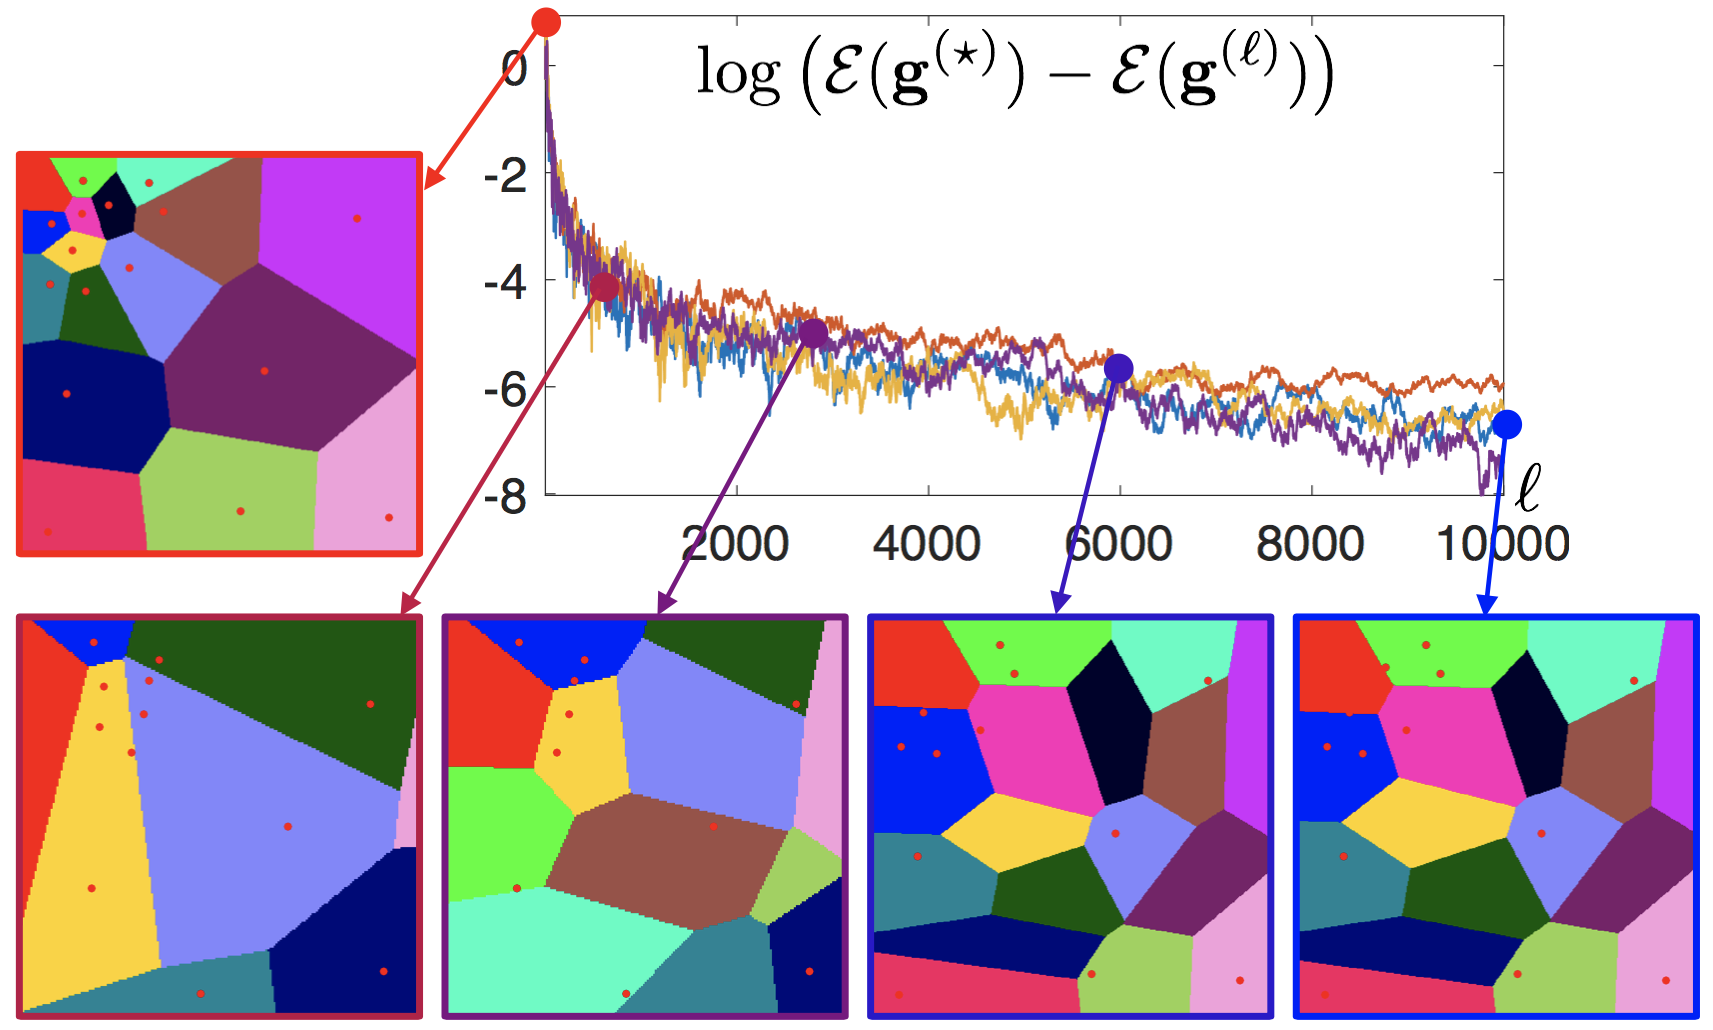
\includegraphics[width=.95\linewidth]{semi-discrete-sgd/semi-discrete-sgd}
\caption{\label{fig-semi-discrete-sgd}
SGD反復~\eqref{eq-sgd}中のエネルギー$\Ee^\epsilon(\it{\gD})$の推移（$\epsilon=0$、正則化なし）。各色付き曲線は異なるランダム化された実行を示す。
%
画像はLaguerreセル$( \Laguerre_{j}(\it{\gD}) )_j$の反復を通じた変化を表示している。
}
\end{figure}

%%%%
\paragraph{平均化を伴う確率的勾配降下法}

SGDはステップサイズ$\tau_\ell$がゼロに速く減衰するため遅い。
%
収束速度を改善するために、過去の反復の平均化が可能であり、これは補助変数$(\it{\tilde\gD})_\ell$に対して「古典的な」SGDを実行することと等価である。
\eq{
	\itt{\tilde\gD} \eqdef  \it{\tilde\gD} + \tau_\ell \nabla_{\gD} E^\epsilon(\it{\tilde\gD},x_\ell),
}
ここで$x_\ell$は$\al$に従って引かれ（すべての$(x_\ell)_\ell$は独立である）、推定される重みベクトルとして平均値を出力する。
\eq{
	\it{\gD} \eqdef \frac{1}{\ell} \sum_{k=1}^\ell  \tilde\gD^{(k)}.
}
これが平均化を伴う確率的勾配降下法（SGA）アルゴリズムを定義する。
%
すべての反復を明示的に保存することを避けるために、以下のように走行平均を更新するだけでよいことに注意されたい：
\eq{
	\itt{\gD} = \frac{1}{\ell+1}  \itt{\tilde\gD} +  \frac{\ell}{\ell+1} \it{\gD}.
}
%
この場合、典型的な減衰の選択はむしろ以下の形である。
\eq{
	\tau_\ell \eqdef \frac{\tau_0}{1 + \sqrt{\ell/\ell_0}}.
}
ステップサイズは~\eqref{eq-step-size-sgd}よりもはるかにゆっくりと、$\ell^{-1/2}$の速度で0に向かうことに注意されたい。
%
\citet{bach2014adaptivity}は、SGAがSGDよりも速い収束（関連する定数が小さい）をもたらすことを証明している。SGDとは対照的に、SGAは汎関数の局所的な強凸性（または最大化問題の場合は強凹性）に適応的であるためである。




%%%%%%%%%%
\begin{rem}[連続-連続問題]\label{rem-sgd-cont-cont}
$\al$も$\be$も離散測度でない場合、問題~\eqref{eq-semi-dual-discr}のような有限次元の双対変数を含む半離散戦略に頼ることはできない。唯一の選択肢は、\citep{genevay2016stochastic}で提案されたように、双対問題~\eqref{eq-dual-entropic}に対して確率的最適化手法を用いることである。その問題の適切な正則化が不可欠であり、例えばエントロピー正則化の強度$\epsilon>0$を設定することで、確率的降下スキームで解ける制約なし問題を得ることができる。
%
問題~\eqref{eq-dual-entropic}を再検討する一つのアプローチは、連続関数の空間上の無限次元最適化問題を、多層ニューラルネットワークで張られるようなはるかに小さな部分集合に制限することである~\citep{seguy2018large}。このアプローチは近似保証のない非凸有限次元最適化問題をもたらすが、高次元のシナリオにおいてWasserstein距離の代理を計算する効果的な方法を提供しうる。
%
もう一つの解決策は、ノンパラメトリック族を用いることであり、これは\citet{genevay2016stochastic}によって提案された再生核Hilbert空間を用いた一種の漸進的精緻化を考えることと等価である。その次元はSGDアルゴリズムの反復回数に比例する。
\end{rem}

% !TEX root = ../ComputationalOTFnT.tex

\todoK{results about embeddings, Will Leeb's work, Naor's work?}
\todoK{Indyk's embeddings for W1}

\chapter{$\Wass_1$ 最適輸送}
\label{c-w1}

本章では、基底コストが距離に等しい最適輸送問題に焦点を当てる。歴史的に、これは~\citeauthor{Monge1781}が\citeyear{Monge1781}年に提起した元来の問題に対応している。この設定は、コンピュータビジョンにおける最適輸送の初期の応用においても、「earth mover's distances」という名称のもとで選ばれたものである~\citep{RubTomGui00}。

基底コストがヒルベルト距離の\emph{二乗}である場合（特に第~\ref{c-dynamic}~章で研究される）とは異なり、コストが距離である輸送問題は理論的に解析がより困難である。
%
注意~\ref{rem-exist-mongemap}は、二乗距離を用いた場合に二つの絶対連続測度間の輸送写像またはカップリングの一意性を述べているが、コストが基底距離そのものである場合、最適カントロヴィッチカップリングは一般に一意ではない。したがって、この状況では一意に定まるモンジュ写像を復元することがしばしば不可能であり、この種の問題は測度の補間には適していない。
%
最適 $\Wass_1$ 輸送計画の存在証明とその幾何学的構造の詳細な解析については、~\citet{trudinger2001monge,caffarelli2002constructing,sudakov1979geometric,evans1999differential}の研究を参照されたい。

理論的には解析がより困難であるものの、線形基底距離を用いた最適輸送は、二次コストよりも外れ値やノイズに対して通常より頑健である。さらに、コストが距離であることにより、局所的なフロー、発散制約、または双対ポテンシャルのリプシッツ性を含む洗練された双対再定式化が可能となり、グラフ理論におけるネットワーク上の\emph{最小費用フロー}手法と整合する、より計算コストの低い数値アルゴリズムが示唆される。
%
この設定はまた、関連するOT距離が任意の分布（正でないものも含む）を比較できるノルムを定義するため、広く利用されている。この性質は、いわゆる\emph{双対ノルム}のより広いクラスに共有されている（詳細は\S\ref{sec-dual-norms}および注意~\ref{rem-unb-dualnorms}を参照）。

%%%%%%%%%%%%%%%%%%
\section{距離空間上の $\Wass_1$}
\label{sec-w1-metric}

ここでは $d$ が $\Xx=\Yy$ 上の距離であると仮定し、基底コスト $c(x,y)=d(x,y)$ を用いてOT問題を解く。以下の命題は、この設定における $c$-変換~\eqref{eq-c-transform}の重要な性質を示す。以下では、関数 $f \in \Cc(\Xx)$ のリプシッツ定数を次のように表す：
\eq{
	\Lip(f) \eqdef \sup \enscond{ \frac{|\f(x)-\f(y)|}{d(x,y)} }{ (x,y) \in \X^2, x \neq y }.
}
$\Lip(f) < +\infty$ を満たす関数 $f$ をリプシッツ関数と定義する。これらは $\Cc(\X)$ の凸部分集合をなす。

\begin{prop}$\X=\Y$ かつ $c(x,y)=d(x,y)$ と仮定する。
このとき、$\f = g^c$ となる $g$ が存在するための必要十分条件は $\Lip(f) \leq 1$ である。
さらに、$\Lip(f)\leq1$ ならば $f^c=-f$ である。
\end{prop}

\begin{proof}
まず、$f=g^c$ と仮定する。このとき、$x,y\in \X$ に対して、
\begin{align*}
|f(x)-f(y)|&=\left|\inf_{z\in\X} d(x,z)-g(z) \;\; - \;\;\inf_{z\in \X} d(y,z)-g(z) \right|\\
&\leq \sup_{z\in\X} |d(x,z)-d(y,z)|\leq d(x,y).
\end{align*}
最初の等号は $g^c$ の定義に従い、次の不等式は恒等式 $|\inf f-\inf g|\leq\sup|f-g|$ に従い、最後の不等式は三角不等式に従う。これにより $\Lip(f)\leq1$ が示される。

次に、$\Lip(f)\leq1$ と仮定し、$g\eqdef -f$ と定義する。リプシッツ性より、すべての $x,y\in\X$ に対して
$f(y)-d(x,y)\leq f(x)\leq f(y)+d(x,y)$ が成り立つ。
これらの不等式を適用すると、
\begin{align*}
g^c(y)&=\inf_{x\in\X}\left[ d(x,y) + f(x) \right]
\geq\inf_{x\in \X} \left[  d(x,y)+f(y)-d(x,y)\right]=f(y),\\
g^c(y)&=\inf_{x\in\X}\left[ d(x,y) + f(x) \right]
\leq \inf_{x\in\X}\left[ d(x,y) + f(y)+d(x,y) \right]=f(y).
\end{align*}
よって、$g=-f$ として $f=g^c$ が成り立つ。同じ不等式を用いると
\begin{align*}
f^c(y)&=\inf_{x\in\X}\left[ d(x,y) - f(x) \right]
\geq\inf_{x\in \X} \left[  d(x,y)-f(y)-d(x,y)\right]=-f(y),\\
f^c(y)&=\inf_{x\in\X}\left[ d(x,y) - f(x) \right]
\leq \inf_{x\in\X}\left[ d(x,y) - f(y)+d(x,y) \right]=-f(y).
\end{align*}
これにより $f^c=-f$ が示される。
\end{proof}

単一ポテンシャルの定式化~\eqref{eq-semi-dual-cont}から出発して、構成を反復し、組 $(\g,\g^c)$ を $(\g^c,(\g^c)^c)$ で置き換えることができる。前の命題より、$(\g^c,-\g^c)$ を用いることができ、これは $\Lip(f) \leq 1$ を満たす任意の組 $(f,-f)$ と等価である。これにより、$\Wass_1$ 距離の以下の代替的な表現が得られる：
%Plugging the relationship $f^c=-f$ into~\eqref{eq-semi-dual-cont} shows
\eql{\label{eq-w1-metric}
	\Wass_1(\al,\be) =
	\umax{f} \enscond{ \int_{\Xx} f(x) (\d\al(x)-\d\be(x)) }{ \Lip(f) \leq 1 }.
}
この表現は、$\Wass_1$ が実際にはノルム、すなわち $\Wass_1(\al,\be) = \norm{\al-\be}_{\Wass_1}$ であることを示しており、$\int_{\Xx} \al=\int_{\Xx} \be$ である限り、任意の測度（必ずしも正でなくてもよい）に対して有効である。このノルムはしばしば\citeauthor{kantorovich1958space}ノルム~\citeyearpar{kantorovich1958space}と呼ばれる。

~\eqref{eq-discr-meas}の形の離散測度に対して、$\al-\be = \sum_{k} \VectMode{m}_k \de_{z_k}$（ただし $z_k \in \Xx$、$\sum_k \VectMode{m}_k=0$）と書くと、最適化~\eqref{eq-w1-metric}は次のように書き直すことができる：
\eql{\label{eq-w1-discr}
	\Wass_1(\al,\be) =
	\umax{ (\fD_k)_k } \enscond{ \sum_k \fD_k \VectMode{m}_k }{ \foralls (k,\ell),
		\abs{\fD_k-\fD_\ell} \leq d(z_k,z_\ell), }
}
これは二次錐制約を持つ有限次元凸計画問題である。これは内点法を用いて、あるいは次に類似の問題について詳述するように、近接法を用いて解くことができる。

$\X=\RR$ 上で $d(x,y)=|x-y|$ を用いる場合、$z_k$ を $z_1 \leq z_2 \leq \ldots$ と順序づけることで制約の数を削減できる。この場合、解くべき問題は
\eq{
	\Wass_1(\al,\be) =
	\umax{ (\fD_k)_k } \enscond{ \sum_k \fD_k \VectMode{m}_k }{ \foralls k, \abs{\fD_{k+1}-\fD_k} \leq z_{k+1}-z_k },
}
となり、これは線形計画問題である。
%
さらに、この1次元の場合、累積分布関数を用いた $\Wass_1$ の閉じた形の表現が~\eqref{eq-w1-1d}で与えられていることに注意されたい。

\begin{rem}[$0<p \leq 1$ の場合の $\Wass_p$]
	$0<p \leq 1$ のとき、$\tilde d(x,y) \eqdef d(x,y)^p$ は三角不等式を満たし、したがって $\tilde d$ 自体が距離となる。このため、上述の $\Wass_1$ に対する結果とアルゴリズムを、$d$ の代わりに $\tilde d$ を用いることで $\Wass_p$ の計算に適用できる。これは、$\Wass_p$ が $p$-ヘルダー関数 $\ensconds{f}{\Lip_p(f) \leq 1}$ の双対であるという主張と等価であり、ここで
	\eq{
		\Lip_p(f) \eqdef \sup \enscond{ \frac{|\f(x)-\f(y)|}{d(x,y)^p} }{ (x,y) \in \X^2, x \neq y }.
	}
\end{rem}

%%%%%%%%%%%%%%%%%%
\section{ユークリッド空間上の $\Wass_1$}
\label{sec-w1-eucl}


ユークリッド空間 $\X=\Y=\RR^\dim$ で $\c(x,y) = \norm{x-y}$ を用いる特別な場合、~\eqref{eq-w1-metric}に現れる大域的リプシッツ制約は、$f$ の勾配に対する一様な上界として局所化できる：
\eql{\label{eq-w1-cont}
	\Wass_1(\al,\be) =
	\umax{f} \enscond{ \int_{\RR^\dim} \f(x) (\d\al(x)-\d\be(x)) }{ \norm{\nabla \f}_\infty \leq 1 }.
}
ここで制約 $\norm{\nabla \f}_\infty \leq 1$ は、任意の点 $x$ における $\f$ の勾配のノルムが $1$ で上から抑えられること、すなわちすべての $x$ に対して $\norm{\nabla \f(x)}_2 \leq 1$ であることを意味する。

~\eqref{eq-w1-cont}の双対問題を考えると、固定された発散制約の下での最適化問題が得られる：
\eql{\label{eq-w1-cont-div}
	\Wass_1(\al,\be) =
	\umin{\flow} \enscond{ \int_{\RR^\dim} \norm{\flow(x)}_2 \d x }{  \diverg(\flow)=\al-\be },
}
これはしばしばベックマンの定式化~\citep{Beckmann52}と呼ばれる。
%
ここでベクトル値関数 $\flow(x) \in \RR^2$ はフロー場として解釈でき、質量の局所的な移動を記述する。二つの入力測度の台の外側では $\diverg(\flow)=0$ であり、これは質量保存の制約である。
%
有限要素を用いて適切に離散化すると、問題~\eqref{eq-w1-cont}および~\eqref{eq-w1-cont-div}は非滑らかな凸最適化問題となる。
%
既成の内点法二次錐最適化ソルバーを使用することもできるが、\S\ref{sec-prox-solvers}で提唱されているように、大規模問題にはより単純だがより適合した一次法の使用が必要である。そこで、例えばダグラス・ラックフォード (DR) 反復~\eqref{eq-dr-iters}や関連する交互方向乗数法を使用できる。一様格子上では、発散制約への射影は高速フーリエ変換を用いて便利に処理できることに注意されたい。これらのアプローチの詳細な説明と三角形メッシュ上のOTへの応用については~\citet{SolomonEMDSurfaces2014}を参照されたい。
%
主双対分離スキームを用いた類似のアプローチについては~\citet{LiRyuOsherYinGangbo2017_parallel,Ryu2017a,Ryu2017b}も参照されたい。
%
双対ポテンシャル $\f$ に対するリプシッツ制約を緩和する近似スキームも提案されている。例えば、ウェーブレット係数に対する制約を用いて明示的な公式を導く手法~\citep{shirdhonkar2008approximate}や、「整流線形」$\max(0,\cdot)$ 活性化関数と制限された重みを持つ多層ニューラルネットワークとしてパラメータ化された関数 $\f$ のみを考える手法~\citep{WassersteinGAN}がある。

%%%%%%%%%%%%%%%%%%
% \section{$\Wass_1$ on Smooth Manifolds}
% \label{sec-w1-manifolds}


%%%%%%%%%%%%%%%%%%
\section{グラフ上の $\Wass_1$}

前述の $\Wass_1$ の定式化~\eqref{eq-w1-cont}および~\eqref{eq-w1-cont-div}は、$\X$ が測地線空間である設定、すなわち $\c(x,y)=\dist(x,y)$（ここで $\dist$ は測地線距離）である場合に一般化できる。$\X$ がリーマン多様体である場合の理論的解析については~\citet{FeldmanMacCann02}を参照されたい。
%
$\X=\range{1,n}$ が離散集合であり、重み（長さ）$\weight_{i,j}$ が付けられた無向辺 $(i,j) \in \Edges \subset \X^2$ を備えている場合、$\X$ が測地線距離（または最短路距離）を備えたグラフであるという重要な場合が得られる：
\eq{
	\distD_{i,j} \eqdef \umin{K \geq 0, (i_k)_k : i \rightarrow j }
	 \enscond{ \sum_{k=1}^{K-1} \weight_{i_k,i_{k+1}} }{ \foralls k \in \range{1,K-1}, (i_k,i_{k+1}) \in \Ee  },
}
ここで $i \rightarrow j$ は $i_1=i$ かつ $i_K=j$ を意味し、すなわちパスが $i$ から始まり $j$ で終わることを示す。

グラフ $\X$ 上の（符号付き）離散測度を定義する二つのベクトル $(\a,\b) \in (\RR^n)^2$ で $\sum_i \a_i = \sum_i \b_i$ を満たすものを考える（これらの重みは正である必要はない）。
%
ここでの目標は、基底距離がグラフの測地線距離である場合に、$p=1$ として~\eqref{eq-wass-p-disc}で導入された $\WassD_1(\a,\b)$ を計算することである。この計算は、$n \times n$ の大きさの「完全な」カップリング $\P$ を計算するまでに至ることなく、代わりにグラフの基礎となる接続性を利用した局所的な作用素に依拠すべきである。これらの作用素は勾配と発散の微分作用素の離散的な定式化である。

離散双対カントロヴィッチポテンシャル $\fD \in \RR^n$ はグラフのすべての頂点で添字づけられたベクトルである。勾配作用素 $\nabla : \RR^n \rightarrow \RR^{\Edges}$ は次のように定義される：
\eq{
	\foralls (i,j) \in \Edges, \quad (\nabla \fD)_{i,j} \eqdef \fD_i-\fD_j.
}
フロー $\flowD = (\flowD_{i,j})_{i,j}$ は辺上で定義され、発散作用素 $\diverg : \RR^{\Edges} \rightarrow \RR^n$（これは勾配 $\nabla$ の随伴作用素）はフローを頂点上で定義されたベクトルに写像し、次のように定義される：
\eq{
	\foralls i \in \range{1,n}, \quad \diverg(\flowD)_i \eqdef \sum_{j: (i,j) \in \Edges} (\flowD_{i,j} - \flowD_{j,i}) \in \RR^n.
}


問題~\eqref{eq-w1-cont}はグラフの設定では次のようになる：
\eql{\label{eq-w1-graph-potential}
	\WassD_1(\a,\b) =
	\umax{\fD \in \RR^n} \enscond{ \sum_{i=1}^n \fD_i (\a_i-\b_i)   }{  \forall (i,j) \in \Edges, \, |(\nabla \fD)_{i,j}| \leq \weight_{i,j}  }.
}
関連する双対問題は、公式~\eqref{eq-w1-cont-div}に対応するものであり、次の通りである：
\eql{\label{eq-w1-graph-div}
	\WassD_1(\a,\b) =
	\umin{\flowD \in \RR_+^\Edges} \enscond{ \sum_{(i,j) \in \Ee} \weight_{i,j} \flowD_{i,j}  }{  \diverg(\flowD)=\a-\b }.
}
これは線形計画問題であり、より正確には最小費用フロー問題のインスタンスである。これを解くために高度に効率的な専用単体法ソルバーが開発されている。例えば~\citep{TreeEMD2007}を参照されたい。% \todoK{detail this}
%
図~\ref{fig-planar-graph}に主問題と双対問題の解の例を示す。
%
定式化~\eqref{eq-w1-graph-div}はいわゆるベックマンの定式化~\citep{Beckmann52}であり、交通渋滞モデルの定義と研究に使用され拡張されてきた。例えば~\citep{CarlierSantambrogioOTCongestion2008}を参照されたい。




\begin{figure}[h!]
\centering
\begin{tabular}{@{}c@{\hspace{10mm}}c@{}}

\includegraphics[width=.45\linewidth]{w1-graph/potential}&

\includegraphics[width=.45\linewidth]{w1-graph/flow}\\
$\fD$ & $({\color{red}\a},{\color{blue}\b})$ および $\flowD$
\end{tabular}
\caption{\label{fig-planar-graph}
一様な重み $\weight_{i,j}=1$ を持つ平面グラフ上での $\WassD_1(\a,\b)$ の計算例。
%
左：~\eqref{eq-w1-graph-potential}の解であるポテンシャル $\fD$（赤から青へ値が増加）。辺の緑色は $|(\nabla \fD)_{i,j}|$ に比例する。
%
右：~\eqref{eq-w1-graph-div}の解であるフロー $\flowD$。太い黒線の辺は非零の $\flowD_{i,j}$ を示し、$\weight_{i,j}=1$ に飽和する。
%
右側のこれらの飽和フロー辺は、左側の $|(\nabla \fD)_{i,j}|=1$ となる薄い緑の辺に対応する。
}
\end{figure}





% !TEX root = ../ComputationalOTFnT.tex

\chapter{動的定式化}
\label{c-dynamic}

この章では、コストが測地距離の二乗である場合の最適輸送の測地線的（動的とも呼ばれる）視点を提示する。これは、二つの測度間の最適輸送を、測度の空間における全長を最小化する曲線として記述するものである。動的な視点は最適輸送の直感的な代替解釈を提供し、流体力学との関連を引き出すだけでなく、二つの密度間の補間を行う際に低次元での OT 計算のための効率的な数値ツールをもたらす。この手法の欠点は、大規模な疎な測度には適用できず、測地距離の二乗コストを用いた正則な領域上の低次元（空間を格子化する必要があるため）でのみ機能することである。

この章では、時刻 $t=0$ の一つの測度から出発して時刻 $t=1$ で別の測度に到達するという考え方に基づき、$(\al,\be)$ の代わりに $(\al_0,\al_1)$ という表記を用いる。

%%%%%%%%%%%%%%%%%%%%%%%%%%%%%%%%%%%%%%%%%
\section{連続定式化}

$\X=\Y=\RR^d$ かつ $c(x,y)=\norm{x-y}^2$ の場合、\eqref{eq-mk-generic}で定義される最適輸送距離 $\Wass_2^2(\al,\be) = \MK_\c(\al,\be)$ は、二つの測度間の最短経路 $(\al_t)_{t=0}^1$ を探索することによって計算できる。
%
この経路は、各時刻で定義されるベクトル場 $\speed_t$ を用いて測度を移流させることで記述される。ベクトル場 $\speed_t$ と経路 $\alpha_t$ は質量保存の公式を満たさなければならず、その結果として
\eql{\label{eq-cons-bb-ncvx}
	\pd{\al_t}{t} + \diverg(\al_t \speed_t) = 0
	\qandq
	\al_{t=0}=\al_0,
	\al_{t=1}=\al_1,
}
が得られる。ここで上式は $\RR^d$ 上の超関数の意味で理解されるべきである。このようなベクトル場の微小長さは、測度 $\al_t$ に付随する $L^2$ ノルムを用いて測定され、次のように定義される。
\eq{\norm{\speed_t}_{L^2(\al_t)} = \left( \int_{\RR^\dim} \norm{\speed_t(x)}^2 \d\al_t(x) \right)^{1/2}.}
この定義は、\citet{benamou2000computational}によって最初に導入された $\Wass_2$ の以下の最短経路再定式化をもたらす：
\eql{\label{eq-bb-non-cvx}
	\Wass_2^2(\al_0,\al_1) = \umin{ (\al_t,\speed_t)_t \text{ sat. \eqref{eq-cons-bb-ncvx}} }
		\int_0^1 \int_{\RR^d}   \norm{\speed_t(x)}^2 \d\al_t(x) \d t,
}
ここで $\al_t$ はスカラー値測度、$\speed_t$ はベクトル値測度である。図~\ref{fig-displacement}にこのような測度の経路の二つの例を示す。


\newcommand{\MyFigDispl}[1]{\includegraphics[width=.19\linewidth]{displacement/#1}}
\begin{figure}[h!]
\centering
\begin{tabular}{@{}c@{\hspace{1mm}}c@{\hspace{1mm}}c@{\hspace{1mm}}c@{\hspace{1mm}}c@{}}
\MyFigDispl{interp-dens-1} &
\MyFigDispl{interp-dens-2} &
\MyFigDispl{interp-dens-3} &
\MyFigDispl{interp-dens-4} &
\MyFigDispl{interp-dens-5} \\
\MyFigDispl{interp-points-1} &
\MyFigDispl{interp-points-2} &
\MyFigDispl{interp-points-3} &
\MyFigDispl{interp-points-4} &
\MyFigDispl{interp-points-5} \\
$\al_0$ & $\al_{1/4}$ & $\al_{1/2}$ & $\al_{3/4}$ & $\al_{1}$
\end{tabular}
\caption{\label{fig-displacement}
\eqref{eq-bb-non-cvx}を満たす変位補間 $\al_t$。
上段：Lebesgue測度に関する密度を持つ二つの測度 $(\al_0,\al_1)$ に対する場合。
下段：同数の点を持つ二つの離散経験測度に対する場合。
}
\end{figure}


定式化~\eqref{eq-bb-non-cvx}は、制約~\eqref{eq-cons-bb-ncvx}が積 $\al_t \speed_t$ を含むため、変数 $(\al_t,\speed_t)_t$ に関して非凸な定式化である。ベクトル値測度（しばしば「運動量」と呼ばれる）
\eq{
	\Moment_t \eqdef \al_t \speed_t,
}
を導入すると、\citeauthor{benamou2000computational}は画期的な論文~\citeyearpar{benamou2000computational}において、次のように書くことで変数 $(\al_t,\Moment_t)_t$ に関して凸になることを示した：
\eql{\label{eq-bb-convex}
	\Wass_2^2(\al_0,\al_1) = \umin{ (\al_t,\Moment_t)_t  \in \BBConstr(\al_0,\al_1)  }
		\int_0^1 \int_{\RR^d} \theta(\al_t(x),\Moment_t(x)) \d x \d t,
}
ここで制約集合を次のように定義する：
\eql{\label{eq-mass-conservation}
	\BBConstr(\al_0,\al_1) \eqdef
	\enscond{ (\al_t,\Moment_t) }{
		\pd{\al_t}{t} + \diverg(\Moment_t) = 0,
		\al_{t=0}=\al_0,
		\al_{t=1}=\al_1
	},
}
また $\theta :  \rightarrow \RR^+ \cup \{+\infty\}$ は以下の下半連続凸関数である：
\eql{\label{eq-theta-dynamic}
	\foralls (a,b) \in \RR_+ \times \RR^\dim, \quad
	\th(a,b) = \choice{
		\frac{\norm{b}^2}{a} \qifq a>0, \\
		0 \qifq (a,b) = 0, \\
		+\infty \quad \text{otherwise}.
	}
}
この定義は一見複雑に見えるかもしれないが、$\al_t(x)=0$ のとき運動量 $\Moment_t(x)$ が消滅すべきことを課すために不可欠である。
%
また、\eqref{eq-bb-convex}は測度 $(\al_t,\Moment_t)$ が密度関数であるかのように非形式的に書かれているが、$\th$ は1次斉次関数であるため（したがって測度がLebesgue測度に関する密度を持たない場合でも定義される）、密度から関数への一意的な拡張が可能であり、これは許容される。

%%%%%%%%%%%%%%%%%%%
%\begin{rem11}{Links with McCann's interpolation}\label{rem-displacement}
\begin{rem11}{McCannの補間との関連}{rem-displacement}
（式~\eqref{eq-brenier-map}の場合のように）$\T_\sharp \al_0=\al_1$ を満たす最適Monge写像 $\T : \RR^\dim \rightarrow \RR^\dim$ が存在する場合、$\al_t$ はMcCannの補間
\eql{\label{eq-mc-cann-interp}
	\al_t = ((1-t) \Id + t \T)_{\sharp} \al_0
}
に等しくなる。
1次元の場合、注意~\ref{rem-1d-ot-generic}を用いると、この補間は次の関係式を用いて計算できる：
\eql{\label{eq-displacement-1d-cumul}
	\cumul{\al_t}^{-1} = (1-t)\cumul{\al_0}^{-1} + t \cumul{\al_1}^{-1};
}
図~\ref{fig-1d-ot}を参照されたい。Wasserstein空間のRiemann幾何学の詳細なレビューについては~\citet{gangbo1996geometry}を参照されたい。
%
最適カップリング $\pi$ がMonge写像の台上にあるとは限らず「単に」最適カップリングが存在する場合には、この補間を次のように計算できる：
\eql{\label{eq-displ-discr}
	\al_t = P_{t\sharp} \pi
	\qwhereq
	P_t : (x,y) \in \RR^\dim \times \RR^\dim \mapsto (1-t) x + t y.
}
例えば、離散的な設定~\eqref{eq-pair-discr}において、$\P$ を~\eqref{eq-mk-discr}の解とすると、補間は次のように定義される：
\eql{\label{eq-mccann-discrete}
	\al_t = \sum_{i,j} \P_{i,j} \de_{ (1-t) x_i + t y_j }.
}
このような補間は通常 $n+m-1$ 個の点上に台を持ち、これは $\P$ の非零要素の最大数である。
%
図~\ref{fig-displacement-emp-weight}に離散測度の変位補間の二つの例を示す。
%
この構成は、$P_t$ を測地線経路に沿った補間に置き換えることで、測地空間 $\Xx$ に一般化できる。
%
McCannの補間は、例えばコンピュータグラフィクスにおける色、形状、照明の補間など、多くの応用がある~\citep{Bonneel-displacement}。
%\end{rem1}
\end{rem11}
%%%%%%%%%%%%%%%%%%%



\newcommand{\MyFigDisplEmp}[1]{\includegraphics[width=.16\linewidth]{interpolation-discrete/empirical/interp-#1}}
\newcommand{\MyFigDisplWei}[1]{\includegraphics[width=.16\linewidth]{interpolation-discrete/weighted/interp-#1}}
\begin{figure}[h!]
\centering
\begin{tabular}{@{}c@{}c@{}c@{}c@{}c@{}c@{}}
\MyFigDisplEmp{1}&
\MyFigDisplEmp{2}&
\MyFigDisplEmp{3}&
\MyFigDisplEmp{4}&
\MyFigDisplEmp{5}&
\MyFigDisplEmp{6}\\
\MyFigDisplWei{1}&
\MyFigDisplWei{2}&
\MyFigDisplWei{3}&
\MyFigDisplWei{4}&
\MyFigDisplWei{5}&
\MyFigDisplWei{6}\\
$\al_0$ & $\al_{1/5}$ & $\al_{2/5}$ & $\al_{3/5}$ & $\al_{4/5}$ & $\al_{1}$
\end{tabular}
\caption{\label{fig-displacement-emp-weight}
離散測度の変位補間~\eqref{eq-displ-discr}の比較。
上段：点群（同数の点を持つ経験測度 $(\al_0,\al_1)$）。
下段：同様であるが重みが変化する場合。$0<t<1$ において、上段の例は $N$ 個の点を持つ経験測度の補間 $\mu_t$ に対応し、下段は $2N-1$ 個の点上に台を持つ測度を定義する。
}
\end{figure}

%%%%%%%%%%%%%%%%%%%%%%%%%%%%%%%%%%%%%%%%%
\section{一様スタガード格子上の離散化}

簡単のため、$\dim=2$ 次元の場合に数値スキームを記述する。より高次元への拡張は直接的である。ここでは~\citet{FPapPeyOud13}によって導入された離散化手法に従い、流体力学で一般的に用いられるスタガード格子技法に触発されたものである。
%
時間を $t_k = k/T \in [0,1]$ と離散化し、空間は点 $x_i = (i_1/n_1,i_2/n_2) \in X = [0,1]^2$ で一様に離散化されるものとする。
%
スタガード格子表現を用いるため、$\al_t$ は時間方向の半格子点に対応する $\a \in \RR^{(T+1) \times n_1 \times n_2}$ で表現され、一方 $\Moment$ は $\MomentD=(\MomentD_1,\MomentD_2)$ で表現される。ここで $\MomentD_1 \in \RR^{T \times (n_1+1) \times n_2}$ と $\MomentD_1 \in \RR^{T \times n_1 \times (n_2+1)}$ は各空間方向の半格子点に格納される。
%
この表現を用いると、$(k,i_1,i_2) \in \range{1,T} \times \range{1,n_1} \times \range{1,n_2}$ に対して、時間微分は
\eq{
	(\partial_t \a)_{k,i} \eqdef \a_{k+1,i}-\a_{k,i}
}
と計算され、空間発散は
\eql{\label{eq-space-diverg-disc}
	\diverg(\MomentD)_{k,i} \eqdef
			\MomentD_{k,i_1+1,i_2}^1-\MomentD_{k,i_1,i_2}^1
			+
			\MomentD_{k,i_1,i_2+1}^2-\MomentD_{k,i_1,i_2}^2,
}
%(assuming $0$ whenever these quantities fall out of the grid)
と計算される。これらはいずれも格子点上で定義され、$\RR^{T \times n_1 \times n_2}$ の配列を形成する。

最適化される汎関数を評価するためには、半格子点から格子点への補間演算子が必要であり、すべての $(k,i_1,i_2) \in \range{1,T} \times \range{1,n_1} \times \range{1,n_2}$ に対して、
\eq{
	\InterpBB_a( \a )_{k,i} \eqdef \InterpBB(\a_{k+1,i},\a_{k,i}),
}
\eq{
	\InterpBB_\Moment( \MomentD )_{k,i} \eqdef (
		\InterpBB(\MomentD_{k,i_1+1,i_2}^1,\MomentD_{k,i_1,i_2}^1),
		\InterpBB(\MomentD_{k,i_1,i_2+1}^2,\MomentD_{k,i_1,i_2}^2)
	 ).
}
最も単純な選択は線形演算子 $\InterpBB(r,s)=\frac{r+s}{2}$ を用いることであり、以下ではこれを考える。\eqref{eq-bb-convex}の離散的な対応物は次のようになる：
\eql{\label{eq-bb-discrete}
	\umin{(\a,\MomentD) \in \BBConstrD(\a_0,\a_1)}
		\Theta(\InterpBB_a(\a),\InterpBB_\Moment( \MomentD )),
}
\eq{
		\qwhereq
		\Theta(\tilde\a,\tilde\MomentD)
		\eqdef \sum_{k=1}^{T} \sum_{i_1=1}^{n_1} \sum_{i_2=1}^{n_2}
		\th( \tilde\a_{k,i}, \tilde\MomentD_{k,i} ),
}
ここで制約は
\eq{
	\BBConstrD(\a_0,\a_1) \eqdef
	\enscond{ (\a, \MomentD)
	}{
		\partial_t \a + \diverg(\MomentD) = 0,
		(\a_{0,\cdot},\a_{T,\cdot}) = (\a_0,\a_1)
	},
}
と表される。ここで $\a \in \RR^{(T+1) \times n_1 \times n_2}$、$\MomentD=(\MomentD_1,\MomentD_2)$ で $\MomentD_1 \in \RR^{T \times (n_1+1) \times n_2}$、$\MomentD_2 \in \RR^{T \times n_1 \times (n_2+1)}$ である。
%
図~\ref{fig-dynamic-maze}にこの離散化スキームを用いて近似された発展 $(\al_t)_t$ の例を示す。

%%%%
\begin{rem}[グラフ上の動的定式化]
$\X$ がグラフで $c(x,y)=d_\X(x,y)^2$ が測地距離の二乗である場合、一様格子離散化~\eqref{eq-space-diverg-disc}の代わりにグラフ構造に対応する離散発散を用いた忠実な離散化手法を導出することが可能である。対応する動的Wasserstein距離に対して熱方程式が勾配流構造を持つことを保証するために（勾配流の詳細については~\S\ref{sec-grad-flows}を参照）、\citet{Maas2011}、その後~\citet{MielkeCVPDE}は対数平均 $\InterpBB(r,s)$ の使用を提案した（\citep{solomon2016continuous,ChowHuangLiZhou2012,chow2017entropy,chow2017discrete}も参照）。
\end{rem}
%%%%

%%%%%%%%%%%%%%%%%%%%%%%%%%%%%%%%%%%%%%%%%
\section{近接作用素ソルバー}
\label{sec-prox-solvers}

離散化された動的OT問題~\eqref{eq-bb-discrete}は、アフィン制約の下での非平滑最適化問題の最小化を要求するため、解くことが困難である。実際、関数 $\th$ は凸であるが、質量が消滅する測度 $\a_{k,i}$ に対しては非平滑である。コンパクトな台を持つ二つの入力測度 $(\a_0,\a_1)$ 間の補間を行う場合、補間された測度 $(\a_{k})_{k=1}^T$ の質量も消滅することが一般に期待され、最適化過程の困難な部分はまさにこの台の発展を追跡することにある。特に、標準的な滑らかな最適化技法を用いることはできない。

\eqref{eq-bb-discrete}を二次錐計画として再定式化する方法はいくつかあり、双対問題を考えるか、あるいは単に汎関数 $\th( \a_{k,i}, \MomentD_{k,i} )$ を制約下の線形関数に置き換えることで実現される：
\eq{
	\Theta(\tilde\a,\tilde\MomentD) = \umin{\tilde \zD} \enscond{
		\sum_{k,i} \tilde \zD_{k,i}
	}{
		\foralls (k,i), (\zD_{k,i},\tilde\a_{k,i},\tilde\MomentD_{i,j}) \in \Ll
	},
}
これには追加変数 $\tilde \zD$ の導入が必要となる。
%
ここで $\Ll \eqdef \ensconds{ (z,a,J) \in \RR \times \RR^+ \times \RR^\dim }{ \norm{J}^2 \leq z a }$ は回転ローレンツ二次錐である。
%
この追加変数により、二次錐計画の標準的な内点法ソルバー~\citep{nesterov1994interior}を用いて離散化問題を解くことが可能となる。これらのソルバーは高速な収束率を持ち、高精度の解を計算できる。しかし、各反復は計算コストが高く、離散化点の数に比例する次元の線形系の求解を必要とする。そのため、画像処理応用で遭遇する大規模多次元問題には適用できない。

これらの高精度ソルバーの代替手段として、低精度の一次手法がある。これらは~\eqref{eq-bb-discrete}のような非平滑だが高度に構造化された問題に適している。この種のソルバーは新しいものではないが、数値精度が主要な目標ではないこれらの応用に最適であるため、画像処理や機械学習の分野で最近再び注目を集めている。
%
これらのソルバーとその大規模応用への使用に関する詳細な説明については、例えばモノグラフ~\citep{BauschkeCombettes11}を参照されたい。
%
ここでは特定のソルバーに集中するが、もちろん他の多くのソルバーも使用可能であり、動的OTに対するいくつかのアプローチの研究については~\citep{FPapPeyOud13}を参照されたい。動的OTに一次スキームを用いるというアイデアは、最初に~\citet{benamou2000computational}によって提案されたことに注意されたい。

DRアルゴリズム~\citep{Lions-Mercier-DR}は、次の形式の非平滑構造化問題を解くために特別に設計されている：
\eql{\label{eq-splitting-opt}
	\umin{x \in \Hh} F(x) + G(x),
}
ここで $\Hh$ はEuclid空間であり、$F, G : \Hh \rightarrow \RR \cup \{+\infty\}$ は二つの閉凸関数で、いわゆる近接作用素
\eql{\label{eq-prox-eucl}
	\foralls x \in \Hh, \quad
	\Prox_{\tau F}(x) \eqdef \uargmin{x' \in \Hh} \frac{1}{2}\norm{x-x'}^2 + \tau F(x)
}
がパラメータ $\tau>0$ に対して「容易に」（閉形式で、または高速に収束するスキームを用いて）計算できるものである。これはEuclid計量に対する近接写像に対応し、$\norm{x-x'}^2$ の代わりにより一般的なBregmanダイバージェンスを用いた定義に拡張できることに注意されたい。$\KLD$ ダイバージェンスを用いた例については~\eqref{eq-prox-kl}を参照されたい。
%
DRアルゴリズムの反復は、初期化 $(x^{(0)}, w^{(0)})\in \Hh^2$ を用いて列 $(\it{x}, \it{w}) \in \Hh^2$ を次のように定義する：
\begin{equation}\label{eq-dr-iters}
\begin{aligned}
	\itt{w} &\eqdef  \it{w} + \al (\Prox_{\ga F} (2\it{x}-\it{w})-\it{x}),\\
	\itt{x} &\eqdef  \Prox_{\ga G}(\itt{w}).
\end{aligned}
\end{equation}
$0 < \al < 2$ かつ $\ga > 0$ ならば、$\it{x} \rightarrow z^\star$ が示され、ここで $z^\star$ は~\eqref{eq-splitting-opt}の解である。詳細は~\citep{Combettes2007}を参照されたい。
%
このアルゴリズムは、もう一つのよく知られた手法である交互方向乗数法~\citep{GabayMercier,GlowinskiMarroco}（レビューについては~\citep{BoydADMM}も参照）と密接に関連しており、これは双対問題にDRを適用することで得られる。二つの手法の等価性（最初に~\citep{Eckstein1992}によって示された）の詳細については~\citep{FPapPeyOud13}を参照されたい。

問題~\eqref{eq-bb-discrete}を形式~\eqref{eq-splitting-opt}に再定式化する方法は多数あり、これらのアプローチの詳細な説明については~\citep{FPapPeyOud13}を参照されたい。簡単な方法として、$x=(\a,\MomentD,\tilde\a,\tilde\MomentD)$ と設定し、
\eq{
	F(x) \eqdef \Theta(\tilde\a,\tilde\MomentD) + \iota_{\BBConstrD(\a_0,\a_1)}(\a,\MomentD)
	\qandq
	G(x) = \iota_{\Dd}(\a,\MomentD,\tilde\a,\tilde\MomentD),
}
\eq{
	\qwhereq \Dd \eqdef \enscond{(\a,\MomentD,\tilde\a,\tilde\MomentD)}{
		\tilde\a=\InterpBB_a(\a), \tilde\MomentD=\InterpBB_\Moment( \MomentD )
	}
}
とする。
%
これら二つの関数の近接作用素は効率的に計算できる。
%
実際、
\eq{
	\Prox_{\tau F}(x) = ( \Prox_{\tau\Theta}(\tilde\a,\tilde\MomentD), \Proj_{\BBConstrD(\a_0,\a_1)}(\a,\MomentD) )
}
が成り立つ。近接作用素 $\Prox_{\tau\Theta}$ は各格子点で三次多項式方程式を解くことで計算される。アフィン制約 $\BBConstrD(\a_0,\a_1)$ への直交射影はPoisson方程式の求解を含み、高速Fourier変換を用いて $O(N\log(N))$ 演算で達成できる。ここで $N=Tn_1 n_2$ は格子点の数である。
%
最後に、近接作用素 $\Prox_{\tau G}$ は線形射影であり、小さな線形系の逆行列計算を必要とする。
%
これらの計算の詳細については~\citet{FPapPeyOud13}を参照されたい。
%
図~\ref{fig-dynamic-maze}に、複雑な平面領域内の動的補間を計算するためにこの手法を用いた例を示す。
%
動的OTに対するこの種の近接法は、平均場ゲーム~\citep{benamou2015augmented}などの関連する問題を解くためにも使用されている。

\begin{figure}[h!]
\centering
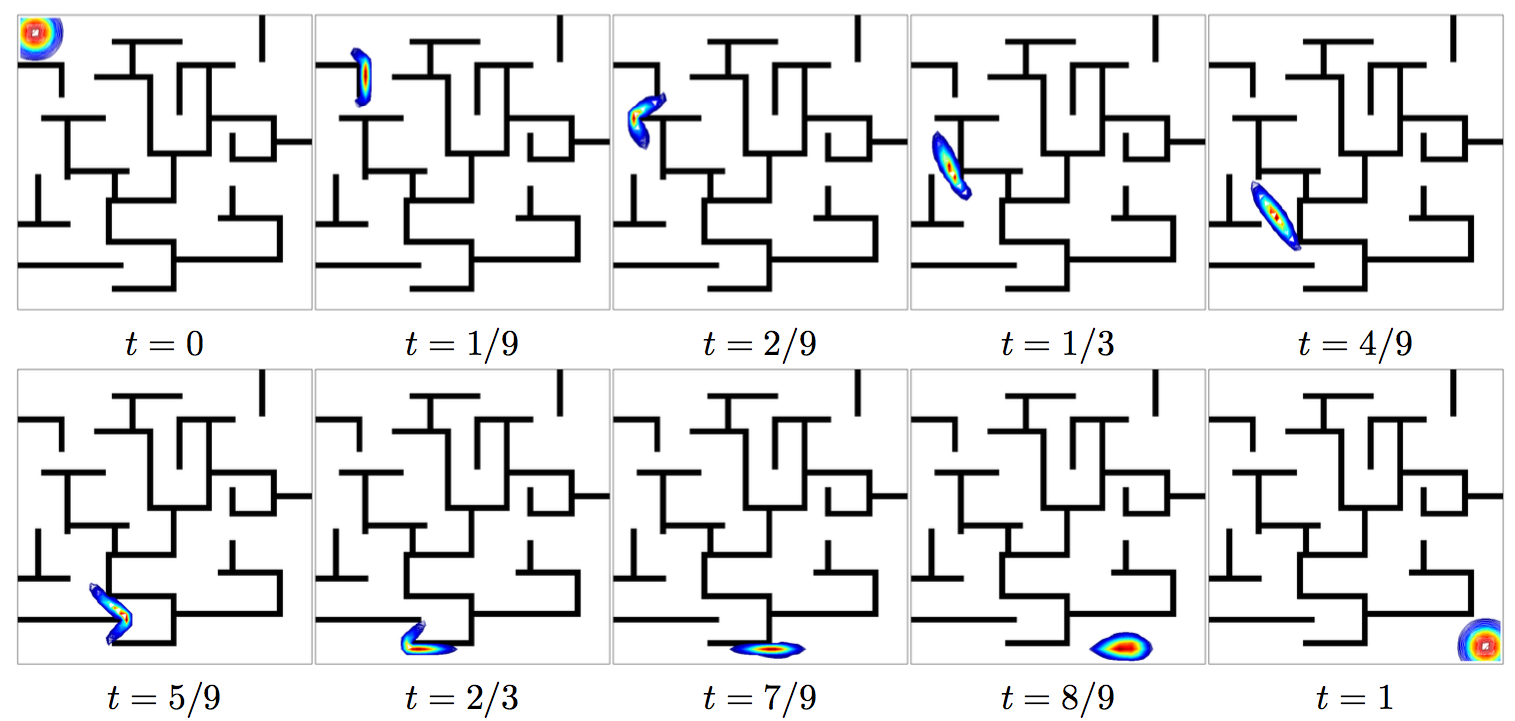
\includegraphics[width=\linewidth]{dynamic/dynamic-maze}
\caption{\label{fig-dynamic-maze}
近接分離スキームを用いて計算された動的OTの解 $\al_t$。
}
\end{figure}



%%%%%%%%%%%%%%%%%%%%%%%%%%%%%%%%%%%%%%%%%
\section{動的非平衡OT}
\label{dynamic-unbalanced}

異なる質量 $\al_0(\Xx) \neq \al_1(\Xx)$ を持つ入力測度を対応付けるため（いわゆる「非平衡」設定、\citet{benamou2003numerical}によって導入された用語）、また局所的な質量変動に対処するため、
%
いくつかの正規化や緩和が提案されている。特に固定周辺分布制約を緩和する方法がある。\S\ref{sec-unbalanced}を参照されたい。
一般的な方法論は、連続の方程式~\eqref{eq-mass-conservation}にソース項 $s_t(x)$ を導入することからなる。したがって次を考える：
\eq{
	\bar\BBConstr(\al_0,\al_1) \eqdef
	\enscond{ (\al_t,\Moment_t,s_t) }{
		\pd{\al_t}{t} + \diverg(\Moment_t) = s_t,
		\al_{t=0}=\al_0,
		\al_{t=1}=\al_1
	}.
}
重要な問題は、このソース項に関連するコストをどのように測定し、元の動的定式化~\eqref{eq-bb-convex}に導入するかである。文献にはいくつかの提案があり、例えば $L^2$ コストを用いるもの~\citet{piccoli2014generalized}がある。
%
質量を「テレポート」すること（無限速度で移動し、それまで質量がなかった領域に突然質量が現れること）を避けるためには、関連するコストは無限大であるべきである。これは、$s_t$ も任意の測度であることを許容し（例えば1次斉次コストを用いて）、$s_t$ を運動量 $\Moment_t$ と同様にペナルティ化することで、単純な凸的方法で達成できることがわかる：
\eql{\label{eq-wfr-dynamic}
	\WFR^2(\al_0,\al_1) = \umin{ (\al_t,\Moment_t,s_t)_t  \in \bar\BBConstr(\al_0,\al_1)  }
		\Theta(\al,\Moment,s),
}
\eq{
	\qwhereq \Theta(\al,\Moment,s) \eqdef
		\int_0^1 \int_{\RR^d} \pa{
			\theta(\al_t(x),\Moment_t(x)) + \tau \theta(\al_t(x),s_t(x))
		}\d x \d t,
}
ここで $\th$ は~\eqref{eq-theta-dynamic}で導入された凸1次斉次関数であり、$\tau$ は質量の輸送と質量の生成/消滅間のトレードオフを制御する重みである。この定式化は複数の著者によって独立に提案された~\citep{LieroMielkeSavareShort,2017-chizat-focm,kondratyev2015}。この「動的」定式化には「静的」な対応物がある。注意~\ref{rem-wfr-static}を参照されたい。
%
凸最適化問題~\eqref{eq-wfr-dynamic}は、\S\ref{sec-prox-solvers}で詳述した方法と類似の手法を用いて解くことができる。
%
図~\ref{fig-unbalanced-dynamic}にいくつかの非平衡OT動的補間の比較を示す。
%
この動的定式化は形状レジストレーションの「メタモルフォーシス」モデル~\citep{Metamorphosis2005}に類似しており、より正確な関連は~\citep{maas2015generalized,maas2016generalized}に詳述されている。

$\tau \rightarrow 0$ かつ $\al_0(\Xx) = \al_1(\Xx)$ の場合、古典的なOT問題が回復され、$\WFR(\al_0,\al_1) \rightarrow \Wass(\al_0,\al_1)$ となる。一方、$\tau \rightarrow +\infty$ の場合、この距離は密度上のヘリンガー計量に近づく：
\begin{align*}
	\frac{1}{\tau}\WFR(\al_0,\al_1)^2\; \overset{\tau \rightarrow +\infty} \longrightarrow
	&\int_{\Xx} | \sqrt{\density{\al_0}(x)} - \sqrt{\density{\al_1}(x)} |^2 \d x \\
	=& \int_{\Xx} | 1 - \sqrt{ \frac{\d\al_1}{\d\al_0}(x) } |^2 \d \al_0(x).
\end{align*}

\begin{figure}[h!]
\centering
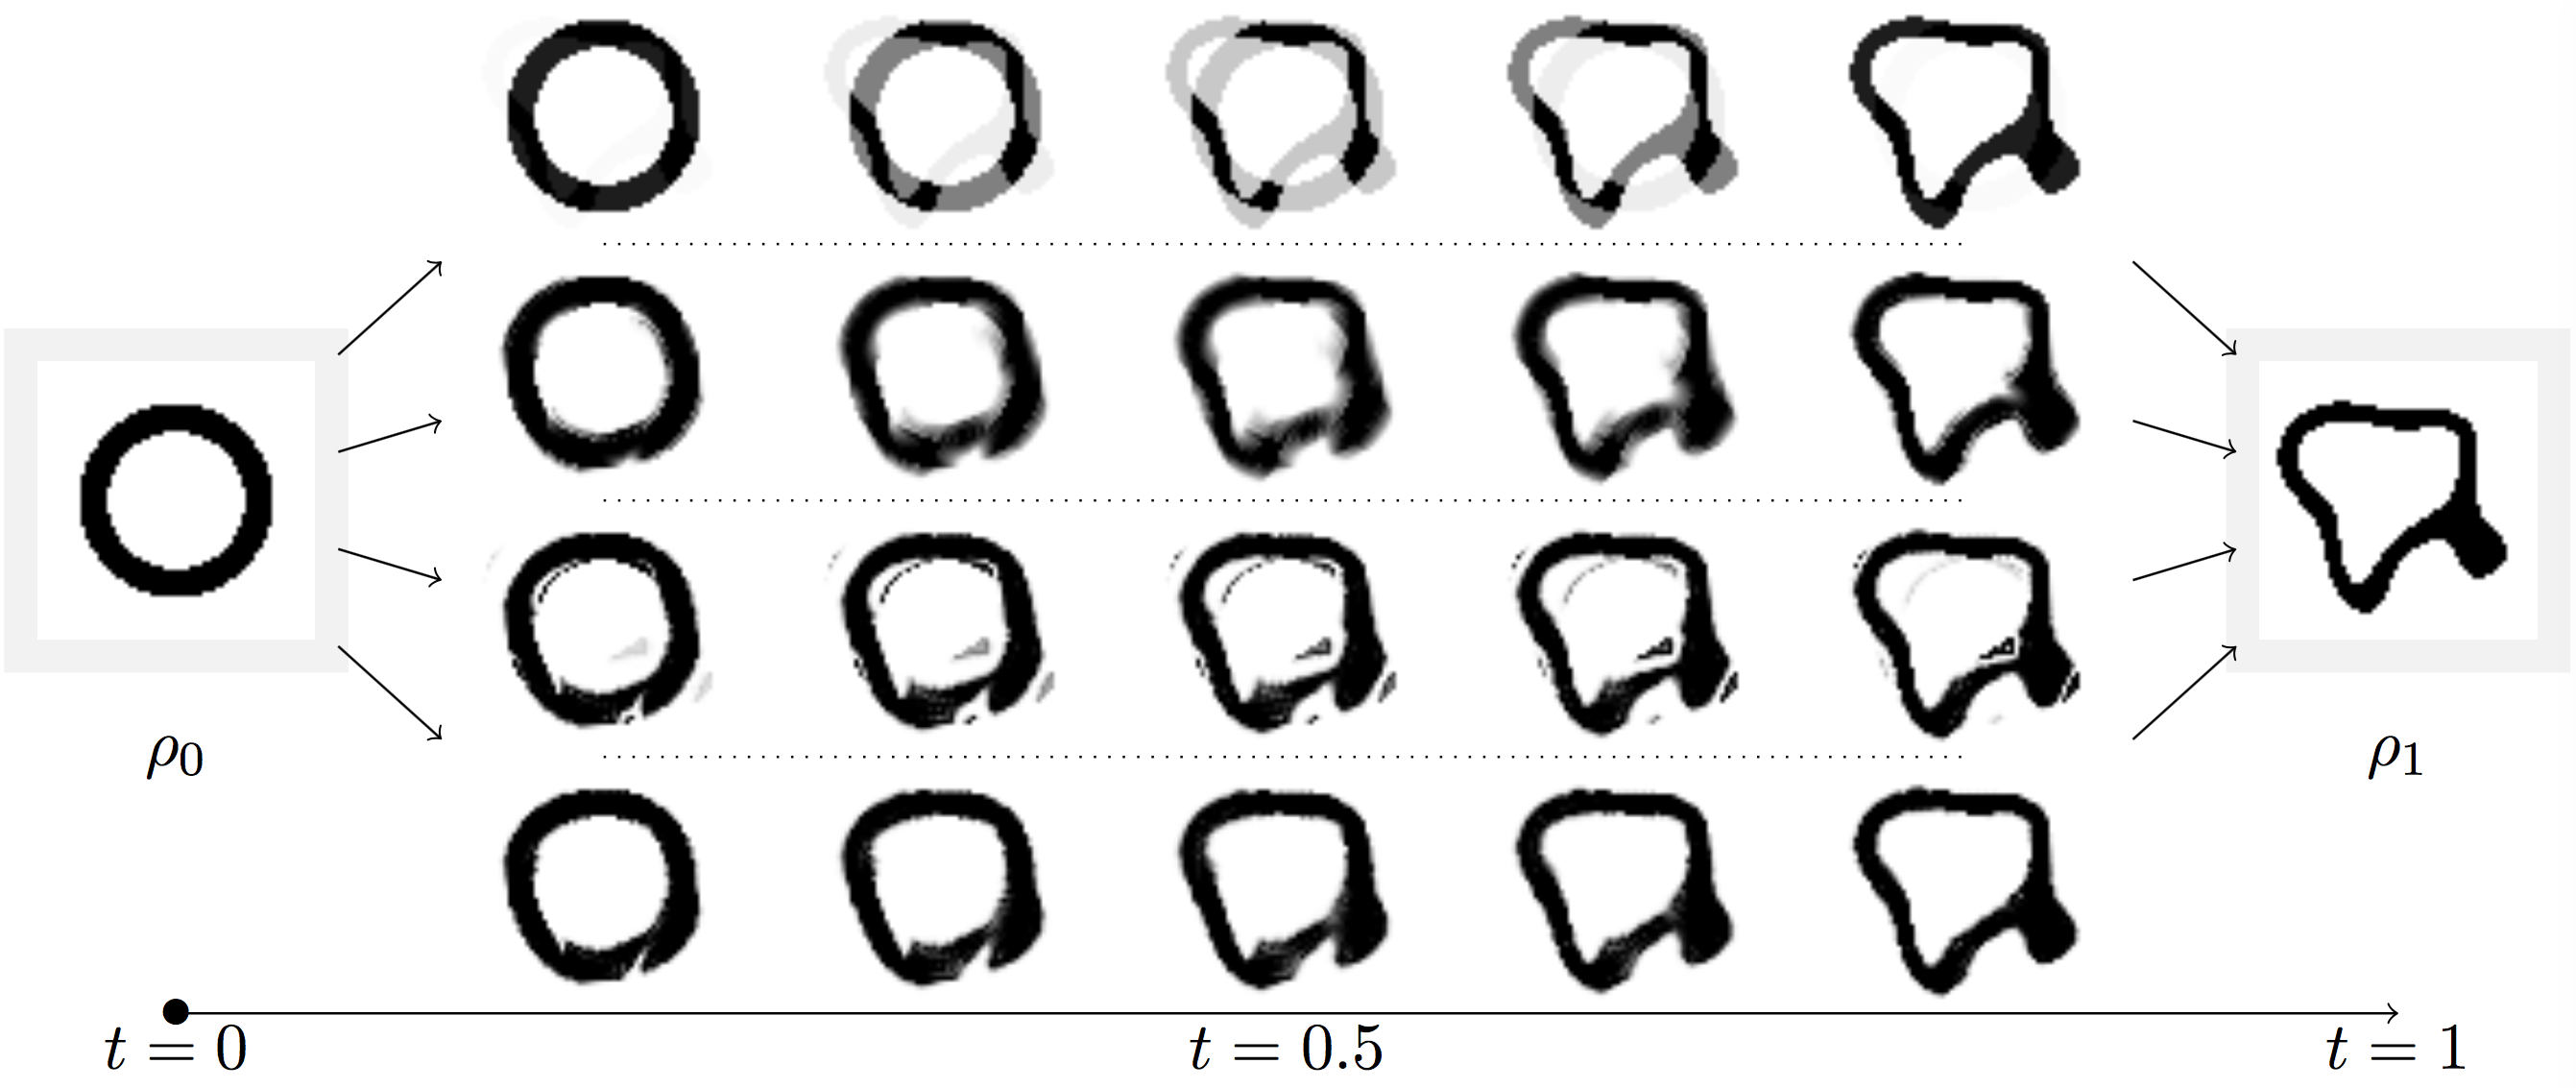
\includegraphics[width=\linewidth]{unbalanced/unbalanced-dynamic}
\caption{\label{fig-unbalanced-dynamic}
ヘリンガー（第1行）、Wasserstein（第2行）、部分最適輸送（第3行）、Wasserstein--Fisher--ラオ（第4行）の動的補間の比較。
}
\end{figure}




%%%%%%%%%%%%%%%%%%%%%%%%%%%%%%%%%%%%%%%%%
\section{より一般的な移動度汎関数}
\label{eq-generic-modibility}

動的定式化~\eqref{eq-bb-convex}を、\eqref{eq-theta-dynamic}で定義されたものの代わりに他の「移動度関数」$\th$ を考えることで一般化することが可能である。この移動度汎関数の可能な選択肢は~\citet{dolbeault2009new}によって提案されている：
\eql{\label{eq?generic-mobility}
	\foralls (a,b) \in \RR_+ \times \RR^\dim, \quad
	\th(a,b) = a^{s-p} \norm{b}^{p},
}
ここでパラメータは $\th$ が凸となるために $p \geq 1$ かつ $s \in [1,p]$ を満たす必要がある。
%
$1<s\leq p$ の場合、$\th$ は無限大で線形増大しないため、\eqref{eq-bb-convex}の解はLebesgue測度に関する密度を持つように制約される必要があり、この定義は注意して扱う必要があることに留意されたい。

$s=1$ の場合は古典的なOT問題に対応し、\eqref{eq-bb-convex}の最適値は $\Wass_p(\al,\be)$ を定義する。この場合、$\th$ は1次斉次であり、\eqref{eq-bb-convex}の解は任意の測度であり得る。$(s=1,p=2)$ の場合は $\Wass_2$ を定義するために~\eqref{eq-bb-convex}で考慮された初期設定である。

極限的な場合 $s=p$ も興味深い。これは双対Sobolevノルム $W^{-1,p}$ に対応し、\eqref{eq-bb-convex}の値は
\eq{
	\norm{\al-\be}_{W^{-1,p}(\RR^\dim)}^p =
	\umin{\f} \enscond{ \int_{\RR^\dim} \f  \d(\al-\be)}{  \int_{\RR^\dim} \norm{ \nabla f(x) }^q \d x \leq 1 }
}
に等しくなる。ここで $1/q+1/p=1$ である。
%
極限 $(p=s,q) \rightarrow (1,\infty)$ では、$\Wass_1$ ノルムが回復される。
%
$s=p=2$ の場合は~\eqref{eq-dual-sobolev-div}で定義されたSobolev $H^{-1}(\RR^\dim)$ Hilbertノルムに対応する。


\todoK{Speak of the connexion with geodesic in shape space~\citet{beg2005computing}. }

\todoK{``Here many computation techniques related to optimal control and Hamilton-Jacobi equations have not mentioned. The connections between optimal transport and Mean field games may be the other interesting direction. Many techniques developed in numerical optimal transport can be applied to general control problems in the set of probability space. For example, a new Hopf-Lax formula is introduced for dynamical optimal transport problem. See related discussions in~\citet{gangbo2008hamilton}.''}



%%%%%%%%%%%%%%%%%%%%%%%%%%%%%%%%%%%%%%%%%
\section{経路空間上の動的定式化}
\label{sec-entropic-dynamic}

古典的OTおよびエントロピー正則化された（\S\ref{c-entropic}を参照）OTの定式化には、空間 $\Xx$ 上のすべての可能な経路 $\ga : [0,1] \rightarrow \Xx$（すなわち曲線）の空間 $\bar\Xx$ 上の抽象的な最適化問題を研究することに基づく、自然な動的定式化が存在する。
%
簡単のため $\Xx=\RR^\dim$ と仮定するが、これは測地空間やグラフなどのより一般的な空間に拡張される。
%
非形式的には、時刻 $t=0,1$ における二つの入力測度 $\al_0,\al_1$ 間の「粒子」の動的挙動は、確率分布 $\bar\pi \in \Mm_+^1(\bar\Xx)$ によって記述される。このような分布は、始点と終点の分布が $(\al_0,\al_1)$ と一致しなければならないという条件を満たすべきであり、これは押し出しを用いて形式的に次のように書かれる：
\eq{
	\bar\Couplings(\al_0,\al_1) \eqdef \enscond{ \bar\pi \in \Mm_+^1(\bar\Xx) }{ \bar P_{0\sharp} \bar\pi = \al_0, \bar P_{1\sharp} \bar\pi = \al_1  },
}
ここで任意の経路 $\ga \in \bar\Xx$ に対して $P_0(\ga) = \ga(0), P_1(\ga) = \ga(1)$ である。

%%%%
\paragraph{経路空間上のOT}

経路空間上で定式化された古典的OT~\eqref{eq-mk-generic}の動的版は次のようになる：
\eql{\label{eq-ot-pathsspace}
	\Wass_2(\al_0,\al_1)^2 =
	\umin{ \bar\pi \in \bar\Couplings(\al_0,\al_1) } \int_{\bar\Xx} \Ll(\ga)^2 \d\bar\pi(\ga),
}
ここで $\Ll(\ga) = \int_0^1 |\ga'(s)|^2 \d s$ は経路 $s \in [0,1] \mapsto \ga(s) \in \Xx$ の運動エネルギーである。それぞれ~\eqref{eq-ot-pathsspace}と~\eqref{eq-mk-generic}を解く最適カップリング $\pi^\star$ と $\bar\pi^\star$ の関連は、$\bar\pi^\star$ が $\pi^\star$ によって規定された割合で点の対を結ぶ測地線にのみ質量を与えることである。離散測度の特別な場合、これは
\eq{
	\pi^\star = \sum_{i,j} \P_{i,j} \de_{(x_i,y_j)}
	\qandq
	\bar\pi^\star = \sum_{i,j} \P_{i,j} \de_{\ga_{x_i,y_j}},
}
を意味する。ここで $\ga_{x_i,y_j}$ は $x_i$ と $y_j$ 間の測地線である。さらに、$\ga$ が $\bar\pi^\star$ に従って抽出されるとき、時刻 $t$ における曲線点 $\ga(t)$ の分布によって定義される測度、すなわち
\eql{\label{eq-interpolation-spacepaths}
	 t \in [0,1] \mapsto \al_t \eqdef P_{t\sharp} \bar\pi^\star
	 \qwhereq
	 P_t(\ga) = \ga(t) \in \Xx,
}
は動的定式化~\eqref{eq-bb-convex}の解、すなわち変位補間である。
%
離散的な場合には、\eqref{eq-mccann-discrete}が回復される。

%%%%
\paragraph{経路空間上のエントロピーOT}

次に、第~\ref{c-entropic}章で定義されたエントロピーOTの、経路空間を用いた再解釈に移る。
%
\eqref{eq-entropic-generic-proj}と同様に、これはKullback--Leiblerダイバージェンスの射影を用いて定義されるが、今回は経路空間上の参照測度 $\bar\Kk$（可逆Brown運動（Wiener過程）の分布であり、初期時刻と最終時刻で一様分布を持つ）に対するものである：
\eql{\label{eq-shrodinger-paths}
	\umin{ \bar\pi \in \bar\Couplings(\al_0,\al_1) } \KL(\bar\pi|\bar\Kk).
}
この問題の概観と~\citet{Schroedinger31}の仕事に関する歴史的説明については、\citet{LeonardSchroedinger}のレビュー論文を参照されたい。
%
\eqref{eq-shrodinger-paths}の（一意的な）解 $\bar\pi_\varepsilon^\star$ は $\varepsilon \rightarrow 0$ のとき~\eqref{eq-ot-pathsspace}の解に収束することが示される。さらに、この解はBrown橋 $\bar\ga_{x,y}^\varepsilon \in \bar\Xx$（ファジーな測地線に類似し、$\varepsilon \rightarrow 0$ で $\de_{\ga_{x,y}}$ に収束する）を用いて、静的エントロピーOT問題~\eqref{eq-entropic-generic}の解と結びつけられる。離散的な設定では、これは
\eql{\label{eq-brownian-bridge-interp}
	\pi_\varepsilon^\star = \sum_{i,j} \P_{\varepsilon,i,j}^\star \de_{(x_i,y_j)}
	\qandq
	\bar\pi_\varepsilon^\star = \sum_{i,j} \P_{\varepsilon,i,j}^\star \bar\ga_{x_i,y_j}^\varepsilon,
}
を意味する。ここで $\P_{\varepsilon,i,j}^\star$ はSinkhornアルゴリズムを用いて計算できる。
%
\eqref{eq-interpolation-spacepaths}と同様に、エントロピー補間を次のように定義できる：
\eq{
	\al_{\varepsilon,t} \eqdef \P_{t\sharp} \bar\pi_\varepsilon^\star.
}
Brown橋に沿った時刻 $t$ における位置の分布 $\P_{t\sharp} \bar\ga_{x,y}^\varepsilon$ は、$\ga_{x,y}(t)$ を中心とする分散 $t(1-t)\varepsilon^2$ のGauss分布 $\Gg_{t(1-t)\varepsilon^2}(\cdot-\ga_{x,y}(t))$ であるから、$\al_{\varepsilon,t}$ は移動するDirac測度の集合のGaussぼかしであることが導かれる：
\eq{
	\al_{\varepsilon,t} =
	\sum_{i,j} \P_{\varepsilon,i,j}^\star \Gg_{t(1-t)\varepsilon^2}( \cdot - \ga_{x_i,y_j}(t) ).
}
得られたBrown橋の混合は図~\ref{fig-schrodinger-dynamic}に表示されている。


% G B D H
\newcommand{\MyFigSchrDyn}[1]{\includegraphics[width=.245\linewidth,trim=50 45 38 35,clip]{schrodinger-dynamic/schrodinger-dynamic-eps#1}}
%%% FIG %%%
\begin{figure}[h!]\centering
\centering
\begin{tabular}{@{}c@{}c@{}c@{}c@{}}
\MyFigSchrDyn{5}&
\MyFigSchrDyn{50}&
\MyFigSchrDyn{200}&
\MyFigSchrDyn{1000}\\
$\varepsilon=0$ & $\varepsilon=.05$ & $\varepsilon=0.2$ & $\varepsilon=1$
\end{tabular}
%%%
\caption{%%%
Schrödingerのエントロピー補間~\eqref{eq-brownian-bridge-interp}に付随する経路空間上のBrown橋経路のサンプル。青は $t=0$ に、赤は $t=1$ に対応する。
} \label{fig-schrodinger-dynamic}
\end{figure}
%%% FIG %%%

このエントロピー補間 $(\al_t)_t$ を記述するもう一つの方法は、Benamou--Brenierの動的定式化~\eqref{eq-bb-non-cvx}の正則化を用いるものであり、すなわち \todoK{check how $\varepsilon$ enters the picture}
\eql{\label{eq-bb-non-cvx-entropy}
	\umin{ (\al_t,\speed_t)_t \text{ sat. \eqref{eq-cons-bb-ncvx}} }
		\int_0^1 \int_{\RR^d}  \pa{
			 \norm{\speed_t(x)}^2  + \frac{\varepsilon}{4} \norm{ \nabla \log(\al_t)(x) }^2
			 }
			 \d\al_t(x) \d t;
}
\citep{gentil2015analogy,chen2016relation}を参照されたい。



% !TEX root = ../ComputationalOTFnT.tex
\newcommand{\myFigRKHS}[1]{\includegraphics[width=.195\linewidth]{rkhs/#1}}
\chapter{統計的ダイバージェンス}
\label{c-statistical}

本章では、Wasserstein距離の統計的性質を考察する。より具体的には、データサイエンスで日常的に用いられる他の主要な距離やダイバージェンスとの比較を行う。二つの確率分布間の距離を、それらの分布からのサンプルのみを用いてどのように近似できるかを定量化する。これらの話題を導入するために、\S\ref{sec-phi-div}と\S\ref{sec-dual-norms}では、それぞれ確率分布間のダイバージェンスと積分確率計量について概説する。ダイバージェンス$D$は典型的には$D(\al,\be) \geq 0$かつ$D(\al,\be)=0$であることと$\al=\be$であることが同値であるが、対称性や三角不等式を満たす必要はない。測度に対する積分確率計量は、所定のテスト関数族を用いて定義される双対ノルムである。これらの量はWasserstein距離に対する健全な代替であり、\S\ref{c-variational}で扱う推論問題に取り組むための損失関数として日常的に用いられている。まず\S\ref{sec-non-embeddability}において、最適輸送距離がHilbert的でないこと、すなわち確率測度の適切な特徴表現上のHilbert計量を用いて効率的に近似することができないことを示す。\S\ref{sec-empirical-wass}では、$\al$と$\be$からそれぞれ抽出された離散サンプル$(x_i)_i$と$(y_j)_j$から$D(\al,\be)$をどのように近似するかを示す。この問題に対する十分な統計的理解は、機械学習においてWasserstein距離を用いる際に不可欠である。なお、本節では主に\emph{連続}集合上に台を持つ分布間の最適輸送の統計的近似を扱う。台空間が有限である場合の同じ問題は、~\citet{sommerfeld2018inference}の研究に続き文献で注目を集めており、~\citet{bigot2017central}によってエントロピー正則化量に拡張されている。


%%%%%%%%%%%%%%%%%%%%%%%%%%%%%%%%%%%%%%%%%%%%%%%%%%%%%%%%%%%%%%%%%%%%%%%%%%%%%%%%%%%%%%%%%%%%%%%%%%%%
%%%%%%%%%%%%%%%%%%%%%%%%%%%%%%%%%%%%%%%%%%%%%%%%%%%%%%%%%%%%%%%%%%%%%%%%%%%%%%%%%%%%%%%%%%%%%%%%%%%%
%%%%%%%%%%%%%%%%%%%%%%%%%%%%%%%%%%%%%%%%%%%%%%%%%%%%%%%%%%%%%%%%%%%%%%%%%%%%%%%%%%%%%%%%%%%%%%%%%%%%
\section{$\phi$-ダイバージェンス}
\label{sec-phi-div}

次節で$\Wass_1$と類似した構成を持つ「弱い」ノルムを詳述する前に、いわゆるダイバージェンスの一般的な構成について説明する。これは確率分布を推定する際の損失関数として利用できる。このようなダイバージェンスは、質量の移動の概念を導入することなく、二つの入力測度をそれらの質量の\emph{各点}比較によって比較する。ダイバージェンスは、二つの測度間の各点の比率を見ることで、それらがどれほど近いかの感覚を与える汎関数である。これらは良好な解析的・計算的性質を持ち、\emph{エントロピー関数}に基づいている。

\begin{defn}[エントロピー関数]
\label{def_entropy}
関数$\phi : \RR \to \RR \cup \{\infty\}$がエントロピー関数であるとは、下半連続かつ凸で、$\dom \phi\subset [0,\infty[$であり、以下の実行可能性条件$\dom \phi \; \cap\;  ]0, \infty[\; \neq \emptyset$を満たすことをいう。$\phi$の無限遠での増大の速度は以下で記述される。%its recession (or horizon) function
\eq{
\phi'_\infty = \lim_{x\rightarrow +\infty} \varphi(x)/x \in \RR \cup \{\infty\} \, .
}
\end{defn}

$\phi'_\infty = \infty$のとき、$\phi$は任意の線形関数より速く増大し、$\phi$は\emph{超線形}であるという。任意のエントロピー関数$\phi$は、以下のように$\phi$-ダイバージェンス（Cisz\'arダイバージェンス~\citep{ciszar1967information,ali1966general}または$f$-ダイバージェンスとも呼ばれる）を誘導する。



\begin{defn}[$\phi$-ダイバージェンス]
\label{def_divergence}
$\phi$をエントロピー関数とする。
$\al,\be \in \Mm(\X)$に対し、$\frac{\d \al}{\d \be} \be + \al^{\perp}$を$\be$に関する$\al$のLebesgue分解\footnote{Lebesgueの分解定理は、$\be$が与えられたとき、$\al$は二つの測度$\al^s + \al^\perp$の和として一意に分解され、$\al^s$は$\be$に関して絶対連続であり、$\al^\perp$と$\be$は互いに特異であることを主張する。}とする。ダイバージェンス$\Divergm_\phi$は以下で定義される。
\eql{\label{eq-phi-div}
	\Divergm_\phi (\al|\be) \eqdef \int_\X \phi\left(\frac{\d \al}{\d \be} \right) \d \be
+ \phi'_\infty \al^{\perp}(\X)
}
ただし$\al,\be$が非負の場合であり、そうでなければ$\infty$とする。
\end{defn}%

~\eqref{eq-phi-div}における追加項$\phi'_\infty \al^{\perp}(\X)$は、$\phi$が無限遠で線形増大を持つ場合でも（例えば、TVノルムを定義する絶対値~\eqref{eq-tv-entropy}の場合のように）、$\Divergm_\phi$が（測度の弱位相に関する）連続汎関数を定義することを保証するために重要である。$\phi$が超線形増大を持つ場合、例えば通常のエントロピー~\eqref{eq-shannon-entropy}では、$\phi'_\infty=+\infty$となるため、$\al$が$\be$に関して密度を持たなければ$\Divergm_\phi (\al|\be) = +\infty$となる。

離散的な設定では、
\eql{\label{eq-div-disc-meas}
	\al=\sum_i \a_i \de_{x_i}
	\qandq \be=\sum_i \b_i \de_{x_i}
}
が$n$個の点$(x_i)_{i=1}^n \subset \X$の同一集合上に台を持つと仮定すると、~\eqref{eq-phi-div}は$\simplex_n$上のダイバージェンスを定義する。
\eql{\label{eq-discr-diverg}
	\DivergmD_\phi(\a|\b) = \sum_{i \in \Supp(\b)} \phi\pa{ \frac{\a_i}{\b_i} } \b_i + \phi'_\infty \sum_{i \notin \Supp(\b)} \a_i,
}
ここで$\Supp(\b) \eqdef \enscond{i \in \range{n}}{ b_i \neq 0 }$である。

以下の命題の証明は~\cite[Thm 2.7]{LieroMielkeSavareLong}に見ることができる。

\begin{proposition}
$\phi$がエントロピー関数であるならば、$\Divergm_\phi$は$(\al,\be)$について同次1次、凸、かつ弱*下半連続である。
\end{proposition}


\begin{figure}[h!]
\centering

\includegraphics[width=.6\linewidth]{divergences/divergences}
\caption{\label{fig-divergences}
エントロピー汎関数の例。
}
\end{figure}


\begin{rem}[双対表現]
	$\phi$-ダイバージェンスは、$\phi$のLegendre変換
	\eq{
		\phi^*(s) \eqdef \usup{t \in \RR} st - \phi(t)
	}
	（~\eqref{eq-legendre}も参照）を用いて以下のように表現できる。
	\eq{
		\Divergm_\phi (\al|\be) = \usup{f: \X \rightarrow \RR} \int_\X f(x) \d\al(x) - \int_\X \phi^*(f(x)) \d\be(x);
	}
	詳細は~\citet{LieroMielkeSavareLong}を参照されたい。
\end{rem}


ここで、この枠組みのいくつかの代表的な例を概観する。図~\ref{fig-divergences}は対応するエントロピー汎関数を示し、図~\ref{fig-divergences-relations}はそれらの関係を概観する。





\begin{figure}[h!]
\centering

\includegraphics[width=.6\linewidth]{divergences/divergences-comparison}
\caption{\label{fig-divergences-relations}
ダイバージェンス間の関係図（~\citet{gibbs2002choosing}に着想を得たもの）。
$\X$を基底距離$d$を持つ距離空間とし、$d_{\max} = \sup_{(x,x')} d(x,x')$を$\X$の直径とする。$\X$が離散的な場合、$d_{\min} \eqdef \min_{x \neq x'} d(x,x')$とする。\todoK{Tripple check these bounds since they might use different definition/normalization. }\todoK{Change the notation for the Hellinger distance one the symbol is decided $\Hellinger$. }
}
\end{figure}


\begin{example}[Kullback--Leiblerダイバージェンス]
\label{ex_KLdiv}
Kullback--Leiblerダイバージェンス$\KL \eqdef \Divergm_{\phi_{\KL}}$は、相対エントロピーとも呼ばれ、既に~\eqref{eq-defn-rel-entropy}と~\eqref{eq-kl-defn}で導入された。これはShannon--Boltzmannエントロピー関数$\phi_{\KL}$に対応するダイバージェンスであり、以下で与えられる。
\eql{\label{eq-shannon-entropy}
	\phi_{\KL}(s)= \begin{cases}
		s\log(s)-s+1 & \textnormal{for } s>0 , \\
		1 & \textnormal{for } s=0 , \\
		+\infty & \textnormal{otherwise.}
		\end{cases}
}
\end{example}

\begin{remark}[Bregmanダイバージェンス]\label{rem-bregman}
離散KLダイバージェンス$\KLD \eqdef \DivergmD_{\phi_{\KL}}$は、$\phi$-ダイバージェンスでありかつBregmanダイバージェンスでもあるという一意的な性質を持つ。
%
$\RR^n$上の離散ベクトルに対して、滑らかな狭義凸関数$\psi : \RR^n \rightarrow \RR$に対応するBregmanダイバージェンス~\citep{bregman1967relaxation}は以下で定義される。
\eql{\label{eq-bregman-discr}
	\VectMode{B}_\psi(\a|\b) \eqdef \psi(\a) - \psi(\b) - \dotp{\nabla \psi(\b)}{\a-\b},
}
ここで$\dotp{\cdot}{\cdot}$は$\RR^n$上の標準内積である。$\VectMode{B}_\psi(\a|\b)$は$\a$の凸関数であり、$\psi$の線形関数であることに注意されたい。
%
$\phi$-ダイバージェンスと同様に、Bregmanダイバージェンスは$\VectMode{B}_\psi(\a|\b) \geq 0$を満たし、$\VectMode{B}_\psi(\a|\b)=0$であることと$\a=\b$であることは同値である。
%
KLダイバージェンスは、~\eqref{eq-discr-entropy}で定義された負のエントロピー$\psi = -\HD$に対するBregmanダイバージェンスであり、すなわち$\KLD = \VectMode{B}_{-\HD}$である。
%
Bregmanダイバージェンスは局所的にはEuclid距離の二乗であり、
\eq{
	\VectMode{B}_\psi(\a + \varepsilon|\a + \eta) = \dotp{ \partial^2 \psi(\a)(\varepsilon-\eta) }{\varepsilon-\eta}
	+ o(\norm{\varepsilon-\eta}^2)
}
が成り立ち、分離点の集合$\enscond{\a}{\VectMode{B}_\psi(\a|\b) = \VectMode{B}_\psi(\a|\b')}$は$\b$と$\b'$の間の超平面である。
%
これらの性質により、Bregmanダイバージェンスは一次最適化法においてEuclid距離の代替として適している。最も有名な例はミラー勾配降下法~\citep{beck2003mirror}であり、これは~\eqref{eq-explicit-metricflow}の形式の陽的降下ステップである。
%
Bregmanダイバージェンスは凸最適化においても重要であり、例えばSinkhorn反復の導出や有限次元での収束の研究に用いることができる。注釈~\ref{rem-iterative-projection}を参照されたい。
%%%% Should be re-written in infinite dimension
%While KL is both a $\phi$ and a Bregman divergence, these are radically different concepts. In particular, to generalize formula~\eqref{eq-bregman-discr} to nondiscrete measures on some space $\Xx$, one needs to fix a reference measure $\xi$ and consider only measures $\al,\be$ with square integrable densities $\frac{\d\al}{\d\xi},\frac{\d\be}{\d\xi} \in L^2(\d\xi)$. For some strictly convex $\psi : L^2(\d\xi) \rightarrow \RR$, one then defines the Bregman divergence as
%\eq{
%	\Bb_{\psi,\xi}(\al|\be) \eqdef \psi\pa{\frac{\d\al}{\d\xi}} -
%		\psi\pa{\frac{\d\be}{\d\xi}} -
%		\int_{\X} \eta(x) \pa{
%			\frac{\d\al}{\d\xi}(x)-\frac{\d\be}{\d\xi}(x)
%		} \d \xi(x),
%}
%where $\eta = \nabla \psi\pa{\frac{\d\be}{\d\xi}}  \in L^2(\d\xi)$ is the gradient~\citep{rao1985cross,jones1990general}.
%%%
%The simplest case is if $\psi(\rho) = \int_\X \tilde\psi(\rho(x)) \d\xi(x)$ in which case
%\eq{
%	\Bb_{\psi,\xi}(\al|\be) \eqdef
%		\int_\X \pa{
%		\tilde\psi\pa{\frac{\d\al}{\d\xi}} -
%		\tilde\psi\pa{\frac{\d\be}{\d\xi}} -
%		\tilde\psi'\pa{\frac{\d\be}{\d\xi}}
%		\pa{
%			\frac{\d\al}{\d\xi}-\frac{\d\be}{\d\xi}
%		}
%		} \d \xi.
%}
\end{remark}

\begin{remark}[KLの双曲幾何]
	Kullback--Leiblerダイバージェンスの幾何学を、Gauss分布の比較における二次最適輸送が定義する幾何学と対比することは興味深い。例えば~\citet{costa2015fisher}が詳述しているように、Kullback--LeiblerダイバージェンスはGauss密度に対して閉じた形を持つ。一変量の場合$\dim=1$において、$\al = \Nn(m_\al,\si_\al^2)$かつ$\be = \Nn(m_\be,\si_\be^2)$とすると、
	\eql{\label{eq-kl-gaussian}
		\KL(\al|\be) = \frac{1}{2}\pa{
			\frac{\si_\al^2}{\si_\be^2}  +
			\log\pa{\frac{\si_\be^2}{\si_\al^2}}
			+ \frac{|m_\al-m_\be|}{\si_\be^2}
			 - 1
		}.
	}
	この表現は、$\si_\be$が$0$に減少し$\be$がDirac質量になるにつれて$\al$と$\be$の間のダイバージェンスが無限大に発散することを示している。この意味で、特異Gauss分布はKL幾何において他のすべてのGauss分布から無限に遠いと言える。したがって、この幾何学は特異共分散を扱うことを避けたい場合に有用である。分析を簡略化するために、KLの無限小幾何学を見ることができ、これは2次のテイラー展開によって得られる。
	\eq{
		\KL( \Nn(m+\de_m,(\si+\de_\si)^2) | \Nn(m,\si^2) ) = \frac{1}{\si^2}\pa{
			\frac{1}{2}\de_m^2 + \de_\si^2
		} +
		o( \de_m^2,\de_\si^2 ).
	}
	この局所Riemann計量、いわゆるFisher計量は、$(m/\sqrt{2},\si) \in \RR \times \RR_{+,*}$上で表現すると、双曲Poincaré半平面の計量と正確に一致する。
	%
	この空間上の測地線は$\si=0$の直線を中心とする半円であり、指数的な速度を持つ。すなわち、極限$\si=0$に到達するのは無限時間後である。
	%
	特に、$\si_\al=\si_\be$であるが$m_\al \neq m_\al$の場合、この双曲半平面上の$(\al,\be)$間の測地線は一定の標準偏差を持たないことに注意されたい。

	Gaussパラメータ$(m,\si)$の空間上のKL双曲幾何学は、注釈~\ref{rem-dist-gaussians}で記述されたOTに付随するEuclid幾何学と対比されるべきである。一変量の場合、
	\eql{\label{eq-univariate-gauss}
		\Wass_2^2( \al,\be ) = |m_\al - m_\be |^2 + |\si_\al-\si_\be|^2.
	}
	図~\ref{fig-kl-gaussians}は、これら二つの幾何学とそれぞれの測地線の視覚的比較を示している。
	%
	この興味深い比較はJean Feydyによって示唆されたものである。
\end{remark}



\begin{figure}[h!]
\centering
\begin{tabular}{@{}c@{\hspace{3mm}}c@{}}

\includegraphics[width=.45\linewidth]{kl-gaussian/interp-kl}&

\includegraphics[width=.46\linewidth]{kl-gaussian/interp-ot}\\
KL & OT
\end{tabular}
\caption{\label{fig-kl-gaussians}
KL（双曲）幾何とOT（Euclid）幾何を用いたGauss分布間の補間の比較。
}
\end{figure}


\begin{example}[全変動]\label{exmp-tv}
全変動距離$\TV \eqdef \Divergm_{\phi_{\TV}}$は、以下に対応するダイバージェンスである。
\eql{\label{eq-tv-entropy}
	\phi_{\TV}(s)= \begin{cases}
		|s-1| & \textnormal{for } s\geq0 , \\
		+\infty & \textnormal{otherwise.}
		\end{cases}
}
これは実際には測度の全空間$\Mm(\X)$上のノルムを定義し、
\eql{\label{eq-defn-tv}
	\TV(\al|\be) = \norm{\al-\be}_{\TV},
	\qwhereq
	\norm{\al}_{\TV} = |\al|(\X) = \int_\X \d|\al|(x).
}
となる。$\al$が$\X=\RR^\dim$上で密度$\density{\al}$を持つ場合、TVノルムは関数の$L^1$ノルムであり、$\norm{\al}_{\TV} = \int_\X |\density{\al}(x)| \d x = \norm{\density{\al}}_{L^1}$となる。
%
$\al$が~\eqref{eq-div-disc-meas}のように離散的である場合、TVノルムは$\RR^n$のベクトルの$\ell^1$ノルムであり、$\norm{\al}_{\TV}=\sum_i |\a_i| = \norm{\a}_{\ell^1}$となる。
\end{example}

\begin{rem}[強位相と弱位相]
	全変動ノルム~\eqref{eq-defn-tv}は測度の空間上のいわゆる「強」位相を定義する。
	%
	半径$R$のコンパクト領域$\X$上では、
	\eq{
		\Wass_1(\al,\be) \leq R \norm{\al-\be}_{\TV}
	}
	が成り立つので、この強い収束の概念はWasserstein距離によって距離化される弱収束を含意する。
	%
	しかし逆は成り立たない。$x \rightarrow y$のとき$\de_x$は$\de_y$に強収束しないからである（$x \neq y$のとき$\norm{\de_x-\de_y}_{\TV}=2$であることに注意）。
	%
	主要な利点は、$\Mm_+^1(\Xx)$が（再びコンパクトな台空間$\X$上で）弱位相に関してコンパクトであることであり、したがって確率測度の任意の列$(\al_k)_k$から常に収束する部分列を取り出すことができる。これにより、第~\ref{c-variational}章で考察するような最適化問題に適した空間となる。
\end{rem}


\begin{example}[Hellinger]\label{exmp-hellinger}
	Hellinger距離$\Hellinger \eqdef \Divergm_{\phi_{H}}^{1/2}$は、以下に対応するダイバージェンスの平方根である。
	\eq{
		\phi_{H}(s)= \begin{cases}
			|\sqrt{s}-1|^2 & \textnormal{for } s\geq0 , \\
			+\infty & \textnormal{otherwise.}
			\end{cases}
	}
	名前が示す通り、$\Hellinger$は$\Mm_+(\X)$上の距離であり、$\norm{\cdot}_{\TV}$と同様に強位相を距離化する。
	%
	$(\al,\be)$が$\X=\RR^\dim$上で密度$(\density{\al},\density{\be})$を持つ場合、$\Hellinger(\al,\be) = \norms{\sqrt{\density{\al}}-\sqrt{\density{\be}}}_{L^2}$となる。
	%
	$(\al,\be)$が~\eqref{eq-div-disc-meas}のように離散的である場合、$\Hellinger(\al,\be) = \norms{\sqrt{\a}-\sqrt{\b}}$となる。
	%
	$\phi_{L^p}(s)=|s^{1/p}-1|^p$を考えるとHellinger（$p=2$）および全変動（$p=1$）距離が一般化され、$\Divergm_{\phi_{L^p}}^{1/p}$は$0<p<+\infty$に対して強収束を距離化する距離となる。
\end{example}


\begin{example}[Jensen--Shannon距離]
	KLダイバージェンスは対称ではなく、Bregmanダイバージェンス（局所的に二次ノルム）ではあるが、距離の二乗ではない。一方、Jensen--Shannon距離$\text{JS}(\al,\be)$は以下で定義され、
	\eq{
		\text{JS}(\al,\be)^2 \eqdef \frac{1}{2}\pa{
			\KL(\al|\xi) + \KL(\be|\xi)
		}
		\qwhereq
		\xi = \frac{\al+\be}{2},
	}
	距離である~\citep{endres2003new,osterreicher2003new}。
	%
	$\text{JS}^2$は$\phi(s) = t\log(t)-(t+1)\log(t+1)$に対する$\phi$-ダイバージェンスであることが示せる。
	%
	$\KL$とは鋭く対照的に、$\text{JS}(\al,\be)$は常に有界である。より正確には、$0 \leq \text{JS}(\al,\be)^2 \leq \ln(2)$を満たす。
	%
	TVノルムやHellinger距離と同様に、強収束を距離化する。
\end{example}



\begin{example}[$\chi^2$]\label{exmp-chisquare}
	$\chi^2$-ダイバージェンス$\chi^2 \eqdef \Divergm_{\phi_{\chi^2}}$は、以下に対応するダイバージェンスである。
	\eq{
		\phi_{\chi^2}(s)= \begin{cases}
			|s-1|^2 & \textnormal{for } s\geq0 , \\
			+\infty & \textnormal{otherwise.}
			\end{cases}
	}
	$(\al,\be)$が~\eqref{eq-div-disc-meas}のように離散的で同一の台を持つ場合、
	\eq{
		\chi^2(\al|\be) = \sum_i \frac{(\a_i-\b_i)^2}{\b_i}.
	}
\end{example}


%%%%%%%%%%%%%%%%%%%%%%%%%%%%%%%%%%%%%%%%%%%%%%%%%%%%%%%%%%%%%%%%%%%%%%%%%%%%%%%%%%%%%%%%%%%%%%%%%%%%
%%%%%%%%%%%%%%%%%%%%%%%%%%%%%%%%%%%%%%%%%%%%%%%%%%%%%%%%%%%%%%%%%%%%%%%%%%%%%%%%%%%%%%%%%%%%%%%%%%%%
%%%%%%%%%%%%%%%%%%%%%%%%%%%%%%%%%%%%%%%%%%%%%%%%%%%%%%%%%%%%%%%%%%%%%%%%%%%%%%%%%%%%%%%%%%%%%%%%%%%%
\section{積分確率計量}
\label{sec-dual-norms}


定式化~\eqref{eq-w1-cont}は双対ノルムの特殊な場合である。双対ノルムは、任意の測度を扱うことのできる「弱い」ノルムを設計するための便利な方法である。可測関数の対称凸集合$B$に対して、以下を定義する。
\eql{\label{eq-dual-norm-cont}
	\norm{\al}_B \eqdef
	\umax{\f} \enscond{ \int_{\X} \f(x) \d\al(x) }{ \f \in B}.
}
これらの双対ノルムは「積分確率計量」と呼ばれることが多い。~\citep{sriperumbudur2012empirical}を参照されたい。


% Cf. ``Integral probability metrics and their generating classes of functions".

\begin{example}[全変動]
全変動ノルム（例~\ref{exmp-tv}）は、連続関数の全空間に対応する双対ノルムである。
\eq{
	B = \enscond{f \in \Cc(\X)}{\norm{f}_\infty \leq 1}.
}
全変動距離は、双対ノルムでもある唯一の非自明なダイバージェンスである。~\citep{sriperumbudur2009integral}を参照されたい。
\end{example}

\begin{rem}[弱収束の距離化]\label{rem-ipm-weak}
より小さな「球」$B$を用いることで、典型的には連続（ときに正則な）関数のみを含む、より弱い双対ノルムが定義される。
%
$\norm{\cdot}_B$が弱収束（定義~\ref{dfn-weak-conv}を参照）を距離化するためには、$B$で張られる空間がsupノルム$\norm{\cdot}_\infty$（すなわち一様収束の位相）に関して連続関数の集合の中で稠密であれば十分である。~\citep[para. 5.1]{ambrosio2006gradient}を参照されたい。
\end{rem}

図~\ref{fig-dual-norms}はいくつかのこのような双対ノルムの比較を示しており、以下で詳述する。


\begin{figure}[h!]
\centering
\begin{tabular}{@{}c@{\hspace{3mm}}c@{}}

\includegraphics[width=.45\linewidth]{dual-norms/1dirac-1dirac} &

\includegraphics[width=.45\linewidth]{dual-norms/1dirac-2dirac} \\
$(\al,\be)=(\de_0,\de_t)$ &
$(\al,\be)=(\de_0,\frac{1}{2}(\de_{-t/2}+\de_{t/2}))$
\end{tabular}
\caption{\label{fig-dual-norms}
双対ノルムの比較。
}
\end{figure}



%%%%
\subsection{$\Wass_1$とフラットノルム}

集合$B$が有界であれば、$\norm{\cdot}_B$は測度の全空間$\Mm(\Xx)$上のノルムとなる。
%
$\Wass_1$の場合はそうではなく、$\int_\X \d\al=0$を満たす$\al$に対してのみ定義される（そうでなければ$\norm{\al}_B=+\infty$となる）。
%
これはポテンシャル$\f$の値に上界を課すことで緩和でき、例えばフラットノルムを定義する。

\begin{example}[$\Wass_1$ノルム]
~\eqref{eq-w1-cont}で定義される$\Wass_1$は、以下を用いる双対ノルム~\eqref{eq-dual-norm-cont}の特殊な場合である。
\eq{
	B = \enscond{f}{\Lip(f) \leq 1}
}
すなわち1-Lipschitz関数の集合である。
\end{example}

\begin{example}[フラットノルムとDudley計量]
フラットノルムは以下を用いて定義される。
\eql{\label{eq-set-flatnorm}
	B=\enscond{f}{\norm{\nabla \f}_\infty \leq 1 \qandq \norm{\f}_\infty \leq 1}.
}
これは測度の全空間$\Mm(\X)$上で弱収束を距離化する。
%
式~\eqref{eq-w1-discr}は、制約$\abs{\fD_k} \leq 1$を追加することでフラットノルムの計算に拡張される。
%
フラットノルムは「Kantorovich--Rubinstein」ノルム~\citep{hanin1992kantorovich}と呼ばれることもあり、画像処理における逆問題の忠実度項として用いられてきた~\citep{lellmann2014imaging}。
%
フラットノルムはDudley計量と類似しており、こちらは以下を用いる。
\eq{\label{eq-set-dudley}
	B=\enscond{f}{\norm{\nabla \f}_\infty + \norm{\f}_\infty \leq 1}.
}
\end{example}


%%%%
\subsection{双対RKHSノルムと最大平均差異}
\label{sec-mmd}


カーネル法、より具体的には再生核Hilbert空間（RKHS; データサイエンスにおける応用の概説は~\citep{scholkopf2002learning}を参照）の機構を用いて、測度上の「Euclid的」ノルム（二次汎関数を用いて構成される）を定義することも可能である。まず基本的な定義を想起する。

\begin{defn}\label{def-negativedefinitekernel}
集合$\X \times \X$上で定義された対称関数$k$（あるいは$\varphi$）が正定値（あるいは負定値）であるとは、任意の$n\geq0$、任意の族$x_1,\dots,x_n\in\Z$、および任意のベクトル$r\in\RR^n$に対して以下の不等式が成り立つことをいう。
\eql{\label{eq-dual-kern}
	\sum_{i,j=1}^n r_i r_j k(x_i,x_j)\geq 0,
	\quad
	\left(\text{resp.}\quad\sum_{i,j=1}^n r_i r_j \varphi(x_i,x_j)\leq 0\right).
}
カーネルが条件付き正定値であるとは、~\eqref{eq-dual-kern}において正定値性が零平均ベクトル$r$（すなわち$\dotp{r}{\ones_n}=0$を満たすもの）に対してのみ成り立つ場合をいう。
\end{defn}


\if 0 %%%% REMOVED
Using a positive definite kernel $k$, one can now define a Hilbertian norm $\norm{\cdot}_\Krkhs$ on functions
\eq{
	\norm{f}_\Krkhs^2 \eqdef \int_{\X \times \X} \Krkhs(x,y) f(x) f(y) \d \rho(x) \d \rho(y)
}
where $\rho$ is some reference measure, typically Lebesgue's measure on $\X=\RR^\dim$. This norm can then be used to define a subset $B$ of functions with bounded RKHS norm,
\eql{\label{eq-dual-rkhs}
	B = \enscond{\f}{ \norm{\f}_\Krkhs \leq 1}
}
%
that is plugged into notation~\eqref{eq-dual-norm-cont}. The dual RKHS norm for measures that results from this construction is often referred to as the ``maximum mean discrepancy'' (MMD) (see~\citet{gretton2007kernel}), and can be revisited through the prism of Kernel Mean Embeddings (see~\citet{muandet2017kernel} for a review).
\fi


$k$が条件付き正定値のとき、以下のノルムが定義される。
\eql{\label{eq-kernel-dual}
	\norm{\al}^2_{\Krkhs} \eqdef \int_{\X \times \X} \Krkhs(x,y) \d \al(x) \d \al(y).
}
これらのノルムは「最大平均差異」（MMD）と呼ばれることが多く（~\citep{gretton2007kernel}を参照）、形状解析では「カーネルノルム」とも呼ばれてきた~\citep{glaunes2004diffeomorphic}。
%
この表現~\eqref{eq-kernel-dual}は、$\X$上の分布$\al$に従う二つの独立な確率ベクトル$(X,X')$を導入して以下のように言い換えることができる。
\eq{
	\norm{\al}^2_{\Krkhs} = \EE_{X,X'}( \Krkhs(X,X') ).
}
$\norm{\cdot}^2_{\Krkhs}$は、$k$に対応するRKHSの単位球$B$に対応する~\eqref{eq-dual-norm-cont}の意味での双対ノルムであることが示される。RKHS関数空間の詳細は~\citep{berlinet03reproducing,Hofmann2008,scholkopf2002learning}を参照されたい。

\begin{rem}[普遍カーネル]
注釈~\ref{rem-ipm-weak}によれば、MMDノルム$\norm{\cdot}_k$は、双対球$B$の張る空間が連続関数の空間$\Cc(\Xx)$の中で稠密であれば弱収束を距離化する。これは、有限和$\sum_{i=1}^n a_i k(x_i,\cdot)$（$n$と点$(x_i)_i$の任意の選択に対して）が一様ノルム$\norm{\cdot}_\infty$に関して$\Cc(\Xx)$の中で稠密であることを意味する。$\X=\RR^d$上の平行移動不変カーネル$\Krkhs(x,y)=\Krkhs_0(x-y)$の場合、これはFourier変換が消えないこと$\hat \Krkhs_0(\om) >0$と同値である。
\end{rem}

$\al$が~\eqref{eq-pair-discr}の形の離散測度である特殊な場合には、以下の簡単な表現が得られる。
\eq{
	\norm{\al}_{\Krkhs}^2 = \sum_{i=1}^n \sum_{i'=1}^n \a_i\a_{i'} \KrkhsD_{i,i'}  = \dotp{\KrkhsD\a}{\a}
	\qwhereq
	\KrkhsD_{i,i'} \eqdef \Krkhs(x_i,x_{i'}).
}
特に、$\al=\sum_{i=1}^n \a_i \de_{x_i}$と$\be=\sum_{i=1}^n \b_i \de_{x_i}$が同一の点集合上に台を持つとき、$\norm{\al-\be}_{\Krkhs}^2 = \dotp{\KrkhsD(\a-\b)}{\a-\b}$となるので、$\norm{\cdot}_{\Krkhs}$は単体$\simplex_n$上のEuclidノルム（$\KrkhsD$が正定値なら真のノルム、$\KrkhsD$が半正定値なら退化したノルム）である。
%
~\eqref{eq-pair-discr}の形の二つの離散測度間の差異を計算するには、以下を用いることができる。
\eql{\label{eq-mmd-discr}
	\norm{\al-\be}_{\Krkhs}^2 =
		\sum_{i,i'} \a_i \a_{i'} \Krkhs(x_i,x_{i'})	+
		\sum_{j,j'} \b_j \b_{j'} \Krkhs(y_j,y_{j'}) - 2
		\sum_{i,j} \a_i \b_j \Krkhs(x_i,y_j).
}

\begin{example}[GaussRKHS]\label{exmp-gaussian-kernel}
最もよく用いられるカーネルの一つはGaussカーネル$\Krkhs(x,y) = e^{-\frac{\norm{x-y}^2}{2 \si^2}}$であり、これは$\Xx=\RR^d$上の正定値普遍カーネルである。
%
Gaussカーネルの魅力的な特徴は、1次元カーネルの積として分離可能であることであり、これにより正則格子上での計算が容易になる（注釈~\ref{rem-separable}も参照）。
しかし、Gaussカーネルを用いる際に生じる重要な問題は、帯域幅パラメータ$\si$を選択する必要があることである。この帯域幅は、比較する測度の観測値間の「典型的なスケール」と一致する必要がある。測度がマルチスケールの特徴を持つ場合（ある領域は非常に密で、他の領域は非常に疎である場合）、Gaussカーネルは適切ではなく、次に詳述する「スケールフリー」カーネルを検討すべきである。このようなスケールフリーカーネルの問題は、大域的（遅い多項式減衰を持つ）であることであり、コンパクト台近似が不可能なため、計算コストが典型的に高くなる。
%
図~\ref{fig-rkhs}はいくつかのカーネルの比較を示している。
\end{example}

\begin{figure}[h!]
\centering
\begin{tabular}{@{}c@{\hspace{0mm}}c@{\hspace{0mm}}c@{\hspace{0mm}}c@{\hspace{0mm}}c@{}}
 &
\myFigRKHS{energy-dist-kernel}&
\myFigRKHS{gaussian-small-kernel}&
\myFigRKHS{gaussian-medium-kernel}&
\myFigRKHS{gaussian-large-kernel}\\
\myFigRKHS{input} &
\myFigRKHS{energy-dist} &
\myFigRKHS{gaussian-small}&
\myFigRKHS{gaussian-medium}&
\myFigRKHS{gaussian-large}\\
$({\color{red} \al},{\color{blue} \be})$ & $\text{ED}(\RR^2,\norm{\cdot})$ & $(G,.005)$ &  $(G,.02)$ & $(G,.05)$
\end{tabular}
\caption{\label{fig-rkhs}
上段: $\norm{\al-\be}_k = \norm{\psi \star (\al-\be)}_{L^2(\RR^2)}$なる$\psi$の表示。Fourier上では$\hat\psi(\om) = \sqrt{ \hat k_0(\om) }$として形式的に定義される。ここで$\Krkhs(x,x')=k_0(x-x')$である。
%
下段: $\psi \star (\al-\be)$の表示。
%
(G,$\si$)は分散$\si^2$のGaussカーネルを表す。$\text{ED}(\RR^2,\norm{\cdot})$のカーネルは$\psi(x)=1/\sqrt{\norm{x}}$である。
%
\todoK{check that in 2D the ED sqrt kernel is $1/\sqrt{|x|}$, I think this is the case.} \todoK{Explain that ED and large sigma are too global to match the feature size, medium sigma only capture one scale of the details ; small sigma too small}
}
\end{figure}


\begin{example}[$H^{-1}(\RR^\dim)$]\label{exp-sobolev-neg1}
もう一つの重要な双対ノルムは$H^{-1}(\RR^\dim)$であり、これは$L^2(\RR^\dim)$に導関数を持つ関数のSobolev空間$H^1(\RR^\dim)$の（超関数上の）双対である。
%
これは主RKHSノルム$\norm{\nabla \f}_{L^2(\RR^\dim)}^2$を用いて定義される。$\dim=1$でない限り、$H^1(\RR^\dim)$のSobolev空間の関数は一般に連続でないため、特異測度（例えばDirac）に対しては定義されない。
%
この$H^{-1}$ノルム（零平均で密度を持つ測度の空間上で定義される）はダイバージェンス形式でも定式化できる。
\eql{\label{eq-dual-sobolev-div}
	\norm{\al-\be}_{H^{-1}(\RR^\dim)}^2 =
	\umin{\flow} \enscond{ \int_{\RR^\dim} \norm{\flow(x)}_2^2 \d x }{  \diverg(\flow)=\al-\be },
}
これは~\eqref{eq-w1-cont-div}と対比されるべきであり、そちらではここで用いた$L^2$ノルムの代わりにベクトル場$\flow$の$L^1$ノルムが用いられていた。
%
このSobolev双対ノルムの「重み付き」版、
\eq{
	\norm{\rho}_{H^{-1}(\al)}^2 =
	\umin{\diverg(\flow)=\rho} \int_{\RR^\dim} \norm{\flow(x)}_2^2 \d \al(x),
}
はWasserstein $\Wass_2$ノルムの自然な「線形化」として解釈できる。すなわち、Benamou--Brenier動的定式化は無限小的に以下のように解釈できる。
\eql{\label{eq-wass-asymp-sob}
	\Wass_2(\al,\al+\varepsilon \rho) = \varepsilon \norm{\rho}_{H^{-1}(\al)} + o(\varepsilon).
}
汎関数$\Wass_2(\al,\be)$と$\norm{\al-\be}_{H^{-1}(\al)}$は同値であることが示される~\citep{peyre2011comparison}。
%
問題は、$\norm{\al-\be}_{H^{-1}(\al)}$がノルムではないこと（$\al$による重み付けのため）であり、$(\al,\be)$が密度を持たない限り、一般にはこれを$\norm{\al-\be}_{H^{-1}(\RR^\dim)}$で置き換えることはできない。
%
この場合、$\al$と$\be$が同一の台上で下から$a>0$、上から$b<+\infty$で有界な密度を持つならば、
\eql{\label{eq-compar-w2-sob}
	b^{-1/2} \norm{\al-\be}_{H^{-1}(\RR^\dim)} \leq W_2(\al,\be) \leq a^{-1/2} \norm{\al-\be}_{H^{-1}(\RR^\dim)};
}
が成り立つ。~\citep[Theo. 5.34]{SantambrogioBook}を参照し、最適定数については~\citep{peyre2011comparison}を参照されたい。
%
% Note however $H^{-1}(\al)$ and $\Wass_2(\al,\be)$ are related when comparing close enough distribution, they have very different behaviors.
\end{example}

\begin{example}[負Sobolev空間]\label{exp-sobolev-neg}
	この構成を一般化するには、任意の負の指数のSobolev空間$H^{-r}(\RR^\dim)$を考えればよい。これは$r$階導関数（超関数の意味で）が$L^2(\RR^\dim)$に属する関数のSobolev空間$H^{r}(\RR^\dim)$の双対である。
	%
	弱収束を距離化するためには、$H^{r}(\RR^\dim)$の関数が連続である必要があり、これは$r>\dim/2$のとき成り立つ。次元$\dim$が増加すると、より高い正則性を考える必要がある。
	%
	任意の$\al$（必ずしも整数でなくてよい）に対して、これらの空間はFourier変換を用いて定義され、Fourier変換$\hat \al(\om)$（ここではLebesgue測度$\d\om$に関する密度として記述）を持つ測度$\al$に対して、
	\eq{
		\norm{\al}_{H^{-r}(\RR^\dim)}^2 \eqdef \int_{\RR^\dim} \norm{\om}^{-2r} |\hat \al(\om)|^{2}\d\om.
	}
	これは$\hat k_0(\om) = \pm \norm{\om}^{-2r}$を持つ畳み込みカーネル$k(x,y)=k_0(x-y)$を用いた双対RKHSノルムに対応する。逆Fourier変換を取ると、（定数を除いて）以下が得られることがわかる。
	 \eql{\label{eq-sob-kern}
	 	\foralls x \in \RR^\dim, \quad
		k_0(x) =
		\choice{
			\frac{1}{\norm{x}^{d-2r}} \qifq r < d/2,  \\
			-\norm{x}^{2r-d} \qifq r>d/2.
		}
	}
\end{example}




\begin{example}[エネルギー距離]\label{exp-energy-dist}
エネルギー距離（$\dim=1$のときCramer距離）~\citep{szekely2004testing}は、距離$\dist$に対して以下で定義される。
\eql{\label{eq-defn-ed}
	\norm{\al-\be}_{\text{ED}(\X,\dist^p)} \eqdef \norm{\al-\be}_{\Krkhs_{\text{ED}}}
	\qwhereq
	\Krkhs_{\text{ED}}(x,y) = -\dist(x,y)^p
}
ただし$0 < p < 2$とする。\todoK{is it correct?}
%
$\dist$が負定値（定義~\ref{def-negativedefinitekernel}を参照）であれば、これは測度上の有効なMMDノルムであり、典型的な例はEuclid距離$\dist(x,y)=\norm{x-y}$である。
%
$\X=\RR^\dim$、$\dist(x,y)=\norm{\cdot}$の場合、~\eqref{eq-sob-kern}を用いると、エネルギー距離はSobolevノルムであることがわかる。
\eq{
	\norm{\cdot}_{\text{ED}(\RR^\dim,\norm{\cdot}^p)} = \norm{\cdot}_{H^{-\frac{d+p}{2}}(\RR^\dim)}.
}
エネルギー距離がGaussカーネル（例~\ref{exmp-gaussian-kernel}）のようなより一般的なカーネルに対して持つ主要な利点は、スケールフリーであり帯域幅パラメータ$\si$に依存しないことである。より正確には、$\X=\RR^\dim$上で因子$s>0$による膨張を$f_s(x)=sx$と記すと、以下のスケーリング挙動を持つ。
\eq{
	\norm{f_{s\sharp}(\al-\be)}_{\text{ED}(\RR^\dim,\norm{\cdot}^p)} = s^{\frac{p}{2}} \norm{\al-\be}_{\text{ED}(\RR^\dim,\norm{\cdot}^p)},
}
一方、Wasserstein距離は完全な線形スケーリングを示す。
\eq{
	\Wass_p( f_{s\sharp}\al,f_{s\sharp}\be) ) = s \Wass_p(\al,\be) ).
}
ただし、エネルギー距離ではパラメータ$p$は$0 < p < 2$を満たす必要があり、$p=2$のときは平均間の距離に退化する。
\eq{
	\norm{\al-\be}_{\text{ED}(\RR^\dim,\norm{\cdot}^2)}
	=
	\norm{\int_{\RR^\dim} x (\d\al(x)-\d\be(x))  },
}
すなわちもはやノルムではない。これは、エネルギー距離ではWasserstein距離と同じ$f_{s\sharp}$下での線形スケーリングを得ることができないことを示している。
%
\todoK{compare the sqrt kernel associated to energy and sobolev and comment its slow decay}
\end{example}





%%%%%%%%%%%%%%%%%%%%%%%%%%%%%%%%%%%%%%%%%%%%%%%%%%%%%%%%%%%%%%%%%%%%%%%%%%%%%%%%%%%%%%%%%%%%%%%%%%%%
%%%%%%%%%%%%%%%%%%%%%%%%%%%%%%%%%%%%%%%%%%%%%%%%%%%%%%%%%%%%%%%%%%%%%%%%%%%%%%%%%%%%%%%%%%%%%%%%%%%%
%%%%%%%%%%%%%%%%%%%%%%%%%%%%%%%%%%%%%%%%%%%%%%%%%%%%%%%%%%%%%%%%%%%%%%%%%%%%%%%%%%%%%%%%%%%%%%%%%%%%
\section{Wasserstein空間はHilbert的ではない}\label{sec-non-embeddability}

\S\ref{sec:specialcases}で先に概説したWasserstein幾何の特殊な場合のいくつかは、最適輸送距離がときに閉じた形で計算できるという事実を明らかにした。またそのような場合に最適輸送距離が確率測度間の\emph{Hilbert的}計量であること、すなわち以下に定義するように、入力測度の空間からHilbert空間への写像$\tphi$が存在することも示した。

\begin{defn}\label{def-Hilbertmetric}
集合$\Z\times \Z$上で定義された距離$d$がHilbert的であるとは、Hilbert空間$\RKHS$と写像$\tphi:\Z\rightarrow \RKHS$が存在して、$\Z$の任意の対$z,z'$に対して$d(z,z')=\|\tphi(z)-\tphi(z')\|_\RKHS$が成り立つことをいう。
\end{defn}

例えば、注釈~\ref{rem-1d-ot-generic}は、Wasserstein計量が一変量分布間のHilbertノルムであることを示している。これは単に$\tphi$を測度にその一般化分位関数を対応させる写像として定義することによる。注釈~\ref{rem-dist-gaussians}は、本章の~\eqref{eq-univariate-gauss}に記されているように、一変量Gauss分布に対して二つの一変量Gauss分布間のWasserstein距離がそれらの平均と標準偏差の間のEuclid距離に過ぎないことを示している。

Hilbert的距離はデータ解析の文脈で用いる際に多くの好ましい性質を持つ~\citep{dattorro2010convex}。第一に、それらは容易に動径基底関数カーネルに変換できる。任意のHilbert的距離$\dist$に対して、$e^{-\dist^p/t}$は任意の$0\leq p\leq 2$と任意の正スカラー$t$に対して正定値カーネルであることが~\citep[Cor. 3.3.3, Prop. 3.2.7]{berg84harmonic}で示されている。Gaussカーネル（$p=2$）とラプラスカーネル（$p=1$）は、通常のEuclid距離を用いたこの結果の単純な応用である。カーネル法の全分野~\citep{Hofmann2008}は、正定値カーネル行列上で動作する凸学習アルゴリズムを定義するために、カーネル関数の正定値性に基づいている。Hilbert空間の点は、多次元尺度構成法~\citep{borg2005modern}のような単純な方法を用いて、低い歪み率で効率的に低次元に埋め込むこともできる~\citep{Johnson84}, \citep[\S V.6.2]{barvinok2002course}。

Hilbert的距離がこのような性質を持つため、Wasserstein距離が上で概説した以上のより一般的な設定、特に$\X$の次元が2以上の場合にもHilbert的であることが期待されるかもしれない。これは以下の同値性を用いて反証できる。

\begin{prop}\label{prop-negative-definite} 距離$d$がHilbert的であることと$d^2$が負定値であることは同値である。
\end{prop}
\begin{proof} 距離がHilbert的であれば、$d^2$が負定値であることは自明である。実際、$\Z$の$n$個の点が与えられると、和$\sum r_i r_j d^2(z_i,z_j)$は$\sum r_i r_j \|\tphi(z_i)-\tphi(z_j)\|_\RKHS^2$と書き直すことができ、$\sum r_i=0$であることを利用して展開すると$-2\sum r_i r_j \dotp{\tphi(z_i)}{\tphi(z_j)}_\RKHS$となり、Hilbert内積の定義により負となる。逆に$d^2$が負定値であれば、$d$がHilbert的であることは\citet{schoenberg38}による重要な結果（\cite[p. 82, Prop. 3.2]{berg84harmonic}に概説）から得られる。
\end{proof}

したがって、以下の命題で述べるように、Wasserstein距離の二乗が負定値でないことを示せば、それがHilbert的でないことを示すのに十分である。

\begin{prop}\label{prop-negative-definite-negative} $\X=\RR^\dim$で$\dim\geq 2$とし、基底コストを$\dist(x,y)=\norm{x-y}_2$とするとき、$p$-Wasserstein距離は$p=1,2$に対してHilbert的でない。
\end{prop}

\begin{proof} $\dim=2$に対して結果を証明すれば十分である。なぜなら、その次元での反例は任意のより高い次元での反例を得るのに十分だからである。$\RR^{2}$の4つのベクトル$x^1, x^2,x^3,x^4$上に台を持つ測度を用いた非確率的な反例を以下のように提示する。$x^{1}=[0,0], x^{2}=[1,0], x^{3}=[0,1], x^{4}=[1,1]$と定義する。次に、4次元の単体上の正則格子のすべての点を$1/4$刻みで考える。単体上にはそのような点が$35=\bigl(\!\bigl(\substack{4\\4}\bigl)\!\bigl)=\binom{4+4-1}{4}$個ある。格子上の各確率ベクトル$\a^i$は、$j\leq 4$に対して$\a^i_j$が集合$\{0,\tfrac{1}{4},\tfrac{1}{2},\tfrac{3}{4},1\}$に属し、$\sum_{j=1}^4\a^i_j=1$を満たす。与えられた$p$に対して、これらのヒストグラム間の$35\times 35$対Wasserstein距離行列$\D_p$が計算できる。$\D_p$が負定値でないことは、その要素ごとの二乗$\D_p^2$について$\J \D_p^2 \J$が正の固有値を持つことと同値であり、ここで$\J$は中心化行列$\J=\Identity_n-\tfrac{1}{n}\ones_{n,n}$である。これは図~\ref{fig-counterexample}に示されている通りである。
\end{proof}

\begin{figure}[h!]
\centering

\includegraphics[width=.6\linewidth]{counterexample_nsdness/maxeig_vs_p}
\caption{\label{fig-counterexample}
距離がHilbert的で\emph{ない}ことは、点集合の対二乗距離行列$\D_p^2$に対応する中心化行列$\J \D_p^2 \J$のスペクトルを見ることで示せる。距離がHilbert的であれば、そのような行列のスペクトルは必然的に非正である。ここでは命題~\ref{prop-negative-definite-negative}の証明で選ばれた点に対して、その行列の最大固有値の値を$p$の種々の値に対してプロットしている。得られた最大固有値を示す。これらの固有値はすべて正であり、これはこれらの$p$のすべての値に対して$p$-Wasserstein距離がHilbert的でないことを示している。
}
\end{figure}



%%%%%%%%%%%%%%%%%%%%%%%%%%%%%%%%%%%%%%%%%%%%%%%%%%%%%%%%%%%%%%%%%%%%%%%%%%%%%%%%%%%%%%%%%%%%%%%%%%%%
\subsection{埋め込みと歪み}

重要な研究の蓄積が、Hilbert的埋め込みを用いたWasserstein距離の近似の困難さを定量化している。
%
$\X=\RR^\dim$で$\dim\geq 2$の場合、測度を$\ell_2$空間に埋め込むと必然的に重要な\todoK{need to be more precise here}歪みが生じることが示されている~(\citet{naor-2005,andoni2015snowflake})。

$0 < p \leq 1$に対して$p$-Wasserstein空間を$\ell_1$に準等長的に埋め込むことは可能であるが（~\citep{indyk,andoni2008earth,do2011sublinear}を参照）、距離間の同値定数は次元$\dim$とともに急速に増大する。なお、$p=1$の場合、埋め込みは離散測度に対してのみ成り立つ（すなわち、埋め込み定数はスパイク間の最小距離に依存する）。\todoK{need to be more precise here}
%
密接に関連する埋め込み手法として、$\Wass_1$のLipschitz関数$f$の双対としての特徴付け（\S\ref{sec-w1-eucl}を参照）を用いて、Lipschitz制約$\norm{\nabla f}_1 \leq 1$をウェーブレット係数上の重み付き$\ell_1$球で近似する方法がある。~\citep{shirdhonkar2008approximate}を参照されたい。
%
このウェーブレット係数の重み付き$\ell_1$球は、いわゆる負の指数のベソフ空間を定義する~\citep{leeb2016holder}。
%
これらの埋め込み結果は、ダイアディック分割を用いたWasserstein距離の上界とも類似している。~\citep[Prop. 1]{weed2017sharp}および~\citep{fournier2015rate}も参照されたい。
%
これは$\ell_1$への準等長的な埋め込みも提供し（この埋め込みはスケーリングされたウェーブレット係数によって与えられる）、入力測度が一様格子上で離散化されている場合にこの埋め込みを線形時間で近似的に計算できるという利点がある。ウェーブレットの詳細は~\citep{mallat2008wavelet}を参照されたい。なお、Wasserstein的距離を計算するためにマルチスケール埋め込みを用いるアイデアは、コンピュータビジョンで広く用いられてきた。例えば~\citep{ling2006diffusion,grauman2005pyramid,CuturiNIPS2006,lazebnik2006beyond}を参照されたい。

%%%%%%%%%%%%%%%%%%%%%%%%%%%%%%%%%%%%%%%%%%%%%%%%%%%%%%%%%%%%%%%%%%%%%%%%%%%%%%%%%%%%%%%%%%%%%%%%%%%%
\subsection{最適輸送の負定値/正定値変種}

後に\S\ref{sec-sliced}で示すように、Wasserstein距離の\emph{スライス}近似、すなわち直線上に射影された測度のランダムな押し出しに対して計算される1次元方向輸送距離の和は、負定値関数の和として負定値である~\citep[\S 3.1.11]{berg84harmonic}。この結果は正定値カーネルを定義するために用いることができる~\citep{kolouri2016sliced}。正定値カーネルを回復する別の方法は、\citet{kosowsky1994invisible}がエントロピー正則化を導入するために提案したように、最適輸送問題を（可能なすべての輸送テーブル上の）最小問題ではなくソフトミン問題として定式化することである。そのソフトミンは、その負の指数関数（母関数とも呼ばれる）が正定値である項を定義する~\citep{cuturi2012positivity}。





%%%%%%%%%%%%%%%%%%%%%%%%%%%%%%%%%%%%%%%%%%%%%%%%%%%%%%%%%%%%%%%%%%%%%%%%%%%%%%%%%%%%%%%%%%%%%%%%%%%%
%%%%%%%%%%%%%%%%%%%%%%%%%%%%%%%%%%%%%%%%%%%%%%%%%%%%%%%%%%%%%%%%%%%%%%%%%%%%%%%%%%%%%%%%%%%%%%%%%%%%
%%%%%%%%%%%%%%%%%%%%%%%%%%%%%%%%%%%%%%%%%%%%%%%%%%%%%%%%%%%%%%%%%%%%%%%%%%%%%%%%%%%%%%%%%%%%%%%%%%%%
\section{OT、MMD、$\phi$-ダイバージェンスの経験的推定量}
\label{sec-empirical-wass}

応用的な設定において、二つの入力測度$(\al,\be) \in \Mm_+^1(\X)^2$が与えられたとき、重要な統計的問題は、$\al$からのサンプル$(x_i)_{i=1}^n$と$\be$からのサンプル$(y_j)_{j=1}^m$のみを用いて（通常は未知の）ダイバージェンス$D(\al,\be)$を近似することである。これらのサンプルはそれぞれの分布から独立同分布に従って抽出されたものと仮定する。

%%%%%%%%%%%%%%%%%%%%%%%%%%%%%%%%%%%%%%%%%%%%%%%%%%%%%%%%%%%%%%%%%%%%%%%%%%
\subsection{OTとMMDの経験的推定量}

Wasserstein距離$\Wass_p$（~\ref{eq-defn-wass-dist}を参照）とMMDノルム（\S\ref{sec-dual-norms}を参照）の両方に対して、分布間の未知の距離の直接的な推定量は、経験的測度間で直接計算することであり、理想的には後者から前者への収束速度を制御できることが望ましい。
\eq{
	D(\al,\be) \approx D(\hat \al_n,\hat \be_m) \qwhereq
	\choice{
		\hat \al_n \eqdef \frac{1}{n}\sum_i \de_{x_i},\\
		\hat \be_m \eqdef \frac{1}{m}\sum_j \de_{y_j}.
	}
}
ここで$\hat \al_n$と$\hat \be_m$はともに確率的測度であるため、$D(\hat \al_n,\hat \be_m)$は確率変数であることに注意されたい。
%
簡単のため、$\X$はコンパクトであると仮定する（非有界領域を扱うには入力測度のモーメントに追加の制約が必要となる）。

弱収束を距離化する（定義~\ref{dfn-weak-conv}を参照）このような双対距離に対して、弱収束$\hat\al_n \rightarrow \al$が成り立つので、$n \rightarrow +\infty$のとき$D(\hat \al_n,\hat \be_n) \rightarrow D(\al,\be)$となる。
%
しかし重要な問題は$D(\hat \al_n,\hat \be_n)$の$D(\al,\be)$への収束速度であり、この速度はしばしば$D$の「サンプル計算量」と呼ばれる。

$D(\al,\be) = \norm{\cdot}_{\TV}$の場合、TVノルムは弱収束を距離化しないため、$\norms{\hat \al_n - \hat \be_n}_{\TV}$は一致推定量ではない。すなわち、$\norm{\al-\be}_{\TV}$に収束しない。実際、確率1で$\norms{\hat \al_n - \hat \be_n}_{\TV}=2$となる。二つの離散測度の台が重ならないからである。同様の問題は他の$\phi$-ダイバージェンスでも生じ、経験的分布間のダイバージェンスを用いて推定することはできない。


%%%%
\paragraph{OTの収束速度}

$\X=\RR^\dim$で有界領域上に台を持つ測度に対して、$\dim>2$かつ$1 \leq p < +\infty$のとき、~\citep{dudley1969speed}により以下が示されている。
\eq{
	\EE( |\Wass_p(\hat \al_n,\hat \be_n)-\Wass_p(\al,\be)| ) = O(n^{-\frac{1}{\dim}}),
}
ここで期待値$\EE$は確率的サンプル$(x_i,y_i)_i$に関してとられている。この速度は、二つの測度の一方がLebesgue測度に関して密度を持つ場合、$\RR^\dim$では最適である。この結果は被覆数の概念を用いて一般の距離空間に対して証明され~\citep{dudley1969speed}、後に特に$\X=\RR^d$の場合に精緻化された~\citep{dereich2013constructive,fournier2015rate}。
% Proof on $\Wass_1$ implies on $\Wass_p$ for $1 \leq p < +\infty$ by monotonicity in $p$.
この速度は、測度が低次元部分領域上に台を持つ場合に精緻化される。~\citet{weed2017sharp}は、実際に速度が台の内在的次元に依存することを示した。\citeauthor{weed2017sharp}はまた、離散的に近似された測度（例えば小さい分散のGauss混合）のような収束の非漸近的挙動も研究した。
%
$\Wass_p(\hat \al_n,\hat \be_n)$のその平均$\Wass_p(\al,\be)$周りへの集中も証明することが可能である。~\citep{bolley2007quantitative,boissard2011simple,weed2017sharp}を参照されたい。

%%%
\paragraph{MMDの収束速度}

~\eqref{eq-kernel-dual}で定義されたRKHSノルムの双対である弱ノルム$\norm{\cdot}^2_{\Krkhs}$（MMDとも呼ばれる）に対して、Wasserstein距離とは対照的に、サンプル計算量は周囲の次元に依存しない。
\eq{
	\EE( |\norms{\hat \al_n-\hat \be_n}_{\Krkhs} - \norm{\al-\be}_{\Krkhs} | ) = O(n^{-\frac{1}{2}});
}
~\citep{sriperumbudur2012empirical}を参照されたい。
%
図~\ref{fig-sample-complexity}はWasserstein距離とMMD距離のサンプル計算量の速度の数値的比較を示している。
%
ただし、$\norms{\hat \al_n-\hat \be_n}_{\Krkhs}^2$は$\norm{\al-\be}_{\Krkhs}^2$のわずかに偏った推定量であることに注意されたい。不偏推定量を定義し、例えばこのような損失の最小化にSGDを使用できるようにするためには、以下の不偏推定量を用いるべきである。
\begin{align*}
	\text{MMD}_{\Krkhs}(\hat \al_n,\hat \be_n)^2 & \eqdef
		\frac{1}{n(n-1)} \sum_{i,i'} \Krkhs(x_i,x_{i'})	+
		\frac{1}{n(n-1)}\sum_{j,j'} \Krkhs(y_j,y_{j'}) \\
		 & \qquad - 2
		\frac{1}{n^2}\sum_{i,j} \Krkhs(x_i,y_j),
\end{align*}
これは~\eqref{eq-mmd-discr}と比較されるべきである。これは$\EE(\text{MMD}_{\Krkhs}(\hat \al_n,\hat \be_n)^2) = \norm{\al-\be}_{\Krkhs}^2$を満たす。~\citep{gretton2012kernel}を参照されたい。


\begin{figure}[h!]
\centering
\begin{tabular}{@{}c@{\hspace{1mm}}c@{}}

\includegraphics[width=.49\linewidth]{sample-complexity/energy-rates-cropped}&

\includegraphics[width=.49\linewidth]{sample-complexity/wass2-rates-cropped}\\
エネルギー距離 $\norm{\cdot}_{H^{-1}}$ & $\Wass_2$
\end{tabular}
\caption{\label{fig-sample-complexity}
$D$が例~\ref{exp-energy-dist}で定義されたエネルギー距離$D=\norm{\cdot}_{H^{-1}}$（すなわち$H^{-1}$ノルム）（左）およびWasserstein距離$D=\Wass_2$（右）の場合の$\log_{10}(n)$の関数としての$\log_{10}(D(\hat\al_n,\hat\al_n'))$の減衰。
%
ここで$(\hat\al_n,\hat\al_n')$は$\al$の二つの独立な経験的分布であり、$\al$は単位立方体$[0,1]^\dim$上の一様分布であり、$\dim \in \{2,3,5\}$のいくつかの値に対して検証されている。
%
網掛け部分は$\log(D(\hat\al_n,\al))$の標準偏差$\pm$での信頼区間を示している。
}
\end{figure}



%%%%%%%%%%%%%%%%%%%%%%%%%%%%%%%%%%%%%%%%%%%%%%%%%%%%%%%%%%%%%%%%%%%%%%%%%%
\subsection{$\phi$-ダイバージェンスの経験的推定量}

離散サンプルから~\eqref{def_divergence}で定義された$\Divergm_\phi(\al|\be)$を$\Divergm_\phi(\hat \al_n|\hat \be_n)$を用いて近似することはできない。実際、この量は$+\infty$であるか（例えば$\KL$ダイバージェンスの場合）、あるいは$n \rightarrow +\infty$のとき$\Divergm_\phi(\al|\be)$に収束しない（例えば$\TV$ノルムの場合）。
%
代わりに、離散的な経験的測度を何らかの方法で平滑化して密度に置き換えるために、密度推定量を用いる必要がある。~\citep{silverman1986density}を参照されたい。
%
Euclid空間$\Xx=\RR^\dim$において、滑らかな窓関数と帯域幅$\si>0$を用いて$h_\si=h(\cdot/\si)$を導入すると、$\al$に対する密度推定量はこのカーネルとの畳み込みによって定義される。
\eql{\label{eq-kernel-density-estimate}
	\hat \mu_n \star h_\si = \frac{1}{n}\sum_i h_\si(\cdot-x_i).
}
%
すると$\phi$ダイバージェンスを以下で近似できる。
\eq{
	\Divergm_\phi^\si(\hat \al_n |\hat \be_n)
	\eqdef
	\frac{1}{n} \sum_{j=1}^n
	\phi\pa{
		\frac{
			\sum_i h_\si(y_j-x_i)
		}{
			\sum_{j'} h_\si(y_j-y_{j'}),
		}
	}
}
ここで$\si$はサンプル数$n$と次元$\dim$に適合させる必要がある。
%
固定帯域幅$\si$の選択を回避し、代わりに最近傍数$k$を選択するノンパラメトリック推定量を考案することも可能である。これらの手法は典型的に最近傍間の距離を利用し~\citep{loftsgaarden1965nonparametric}、これは帯域幅$\si$を局所サンプリング密度に局所的に適応させることに類似する。$\De_k(x)$を$x \in \RR^\dim$と$(x_i)_{i=1}^n$の中のその第$k$最近傍との距離とすると、密度推定量は以下で定義される。
\eql{\label{eq-knn-density-estimate}
	\rho_{\hat \al_n}^k(x) \eqdef \frac{k/n}{ |B_\dim| \De_k(x)^r },
}
ここで$|B_\dim|$は$\RR^\dim$における単位球の体積である。
%
~\eqref{eq-kernel-density-estimate}において幅$\si$の領域内に落ちるサンプル数を何らかの方法で「数える」代わりに、この式~\eqref{eq-knn-density-estimate}は$k$個のサンプルを包含するのに必要な半径を推定する。図~\ref{fig-density-estimation}は推定量~\eqref{eq-kernel-density-estimate}と~\eqref{eq-knn-density-estimate}を比較している。
%
典型的な応用例は~\eqref{eq-discr-entropy}でエントロピー汎関数（Lebesgue測度に関するKLダイバージェンス）について詳述されている。詳細は~\citep{BerishaHero}を参照されたい。


\newcommand{\myFigDE}[1]{\includegraphics[width=.32\linewidth]{density-estimation/#1}}

\begin{figure}[h!]
\centering
\begin{tabular}{@{}c@{\hspace{1mm}}c@{\hspace{1mm}}c@{}}
\myFigDE{kernel-1} & \myFigDE{kernel-3} & \myFigDE{kernel-5} \\
$\si=2.5 \cdot 10^{-3}$ & $\si=15 \cdot 10^{-3}$ & $\si=25 \cdot 10^{-3}$ \\
\myFigDE{nn-1} & \myFigDE{nn-3} & \myFigDE{nn-5} \\
$k=1$ & $k=50$ & $k=100$
\end{tabular}
\caption{\label{fig-density-estimation}
二つのGauss分布の混合からの$n=200$サンプルに対する、カーネル密度推定$\hat \mu_n \star h_\si$（上段、Gaussカーネル$h$を使用）と$k$-最近傍推定$\rho_{\hat \al_n}^k$（下段）の比較。
}
\end{figure}



%%%%%%%%%%%%%%%%%%%%%%%%%%%%%%%%%%%%%%%%%%%%%%%%%%%%%%%%%%%%%%%%%%%%%%%%%%%%%%%%
%%%%%%%%%%%%%%%%%%%%%%%%%%%%%%%%%%%%%%%%%%%%%%%%%%%%%%%%%%%%%%%%%%%%%%%%%%%%%%%%
%%%%%%%%%%%%%%%%%%%%%%%%%%%%%%%%%%%%%%%%%%%%%%%%%%%%%%%%%%%%%%%%%%%%%%%%%%%%%%%%
\section{エントロピー正則化：OTとMMDの間}
\label{sec-entropy-ot-mmd}

命題~\ref{prop-sinkhorn-div}に従い、Sinkhornダイバージェンスは以下で定義されることを想起する。
\eq{
	\SINKHORNP_\C^\varepsilon(\a,\b) \eqdef
	\dotp{\P^\star}{\C} =
	\dotp{e^{\frac{\fD^\star}{\varepsilon}}}{(\K\odot \C)e^{\frac{\gD^\star}{\varepsilon}}},
}
ここで$\P^\star$は~\eqref{eq-regularized-discr}の解であり、$(\fD^\star,\gD^\star)$は~\eqref{eq-dual-formulation}の解である。
%
ある距離$\dist$に対して$\C_{i,j}=\dist(x_i,x_j)^p$と仮定すると、~\eqref{eq-pair-discr}の形の二つの離散確率分布に対して、これは正則化されたWassersteinコストを定義する。
\eq{
	\Wass_{p,\varepsilon}(\al,\be)^p \eqdef \SINKHORNP_\C^\varepsilon(\a,\b).
}
この定義は任意の入力分布（必ずしも離散的でなくてよい）に以下のように一般化される。
\eq{
	\Wass_{p,\varepsilon}(\al,\be)^p \eqdef \int_{\X \times \X} \dist(x,y)^p \d\pi^\star(x,y),
}
ここで$\pi^\star$は~\eqref{eq-entropic-generic}の解である。

正則化によって導入されるバイアス（特に$\Wass_{p,\varepsilon}(\al,\al) \neq 0$）を打ち消すために、補正された正則化ダイバージェンスを導入する。
\eq{
	\tilde\Wass_{p,\varepsilon}(\al,\be)^p \eqdef
	2 \Wass_{p,\varepsilon}(\al,\be)^p
	-
	\Wass_{p,\varepsilon}(\al,\al)^p
	-
	\Wass_{p,\varepsilon}(\be,\be)^p.
}
$e^{-c/\epsilon}$が正定値カーネルであれば、関連する補正されたダイバージェンス（$\SINKHORNP_\C^\varepsilon$の代わりに$\MKD_\C^\varepsilon$を用いて得られるもの）は正であることが~\citep{feydy2018interpolating}で証明されている。
%
例えば~\citet{amari2017information}が提案しているように、正則化最適輸送を用いた他の再正規化スキームを定義することも可能であることに注意されたい。

\begin{figure}[h!]
\centering
\begin{tabular}{@{}c@{\hspace{1mm}}c@{}}

\includegraphics[width=.49\linewidth]{sample-complexity-regul/influ-epsilon-d2-cropped}&

\includegraphics[width=.49\linewidth]{sample-complexity-regul/influ-epsilon-d5-cropped}\\
$\dim=2$ & $\dim=5$
\end{tabular}
\caption{\label{fig-sample-complexity-regul}
種々の$\varepsilon$に対する$p=3/2$での$\EE(\log_{10}(\tilde\Wass_{p,\varepsilon}(\hat\al_n,\hat\al_n')))$の$\log_{10}(n)$の関数としての減衰。ここで$\al$は図~\ref{fig-sample-complexity}と同じものである。\todoK{redo the plot with higher precision}
}
\end{figure}


以下の命題は~\citep{ramdas2017wasserstein}に証明があり、この正則化ダイバージェンスが例~\ref{exp-energy-dist}で定義されたWasserstein距離とエネルギー距離の間を補間することを示している。

\begin{prop}
	以下が成り立つ。
	\eq{
		\tilde\Wass_{p,\varepsilon}(\al,\be)  \overset{\varepsilon \rightarrow 0}{\longrightarrow} 2 \Wass_{p}(\al,\be)
		\qandq
		\tilde\Wass_{p,\varepsilon}(\al,\be)^p \overset{\varepsilon \rightarrow +\infty}{\longrightarrow} \norm{\al-\be}_{\text{ED}(\X,\dist)}^2,
	}
	ここで$\norm{\cdot}_{\text{ED}(\X,\dist)}$は~\eqref{eq-defn-ed}で定義されている。
\end{prop}

図~\ref{fig-sample-complexity-regul}は$\epsilon$のサンプル計算量の速度への影響を数値的に示している。$\Xx=\RR^d$上で$c(x,y)=\norm{x-y}^2$の場合、これらの速度がOTとMMDの速度の間を補間することが~\cite{genevay2018sample}で証明されている。





% !TEX root = ../ComputationalOTFnT.tex

\chapter{変分ワッサーシュタイン問題}
\label{c-variational} % a label for the chapter, to refer to it later

データ解析において、確率測度間の一般的なダイバージェンス（\emph{例：}ユークリッド、全変動、ヘリンガー、カルバック・ライブラー）は、パラメータ推定問題におけるフィッティング誤差や損失の測定によく用いられる。本章に至るまで、我々は最適輸送幾何学が他の情報ダイバージェンスにはない固有の能力、すなわち物理的な概念（質量の移動）と幾何学（観測値やビン間のグラウンドコスト）を活用して測度を比較する能力を持つことを論じてきた。これら二つの事実を組み合わせると、ワッサーシュタイン距離を損失関数として使用することは非常に魅力的となる。このアイデアは近年、様々な応用問題に対して探究されてきた。しかし、このアイデアに伴う主な技術的課題は、ワッサーシュタイン距離を効率的に近似し微分することにある。本章ではいくつかの動機付けとなる例から始め、本書の前半の章で提示した様々な数値スキームが変分ワッサーシュタイン問題を解くためにどのように利用できるかを示す。

画像処理において、ワッサーシュタイン距離はテクスチャ合成の損失として使用でき~\citep{2016-tartavel-siims}、合成されたサンプルと入力サンプルの統計量間の不一致を考慮する。また、画像領域の統計的均質性を考慮した画像セグメンテーションにも使用される~\citep{SchnorSegmentation,RabinPapadakisSSVM,peyre2012wasserstein,ni2009local,schmitzer2013object,liimage}。
%
ワッサーシュタイン距離はまた、測定値が確率測度である逆問題に対する非常に自然な適合度項でもある。例えば、画像復元~\citep{lellmann2014imaging}、トモグラフィック反転~\citep{AbrahamRadon}、密度正則化~\citep{Burger-JKO}、粒子画像流速計測~\citep{saumier2015optimal}、スパース回復と圧縮センシング~\citep{indyk2011k}、および地震波インバージョン~\citep{metivier2016optimal}がある。
%
測度間の距離（主に\S\ref{sec-mmd}で示されるカーネルベースのもの）は、計算解剖学~\citep{vaillant2005surface}における形状マッチング（リフトされた空間上の測度として表現され、しばしばカレントと呼ばれる）に日常的に使用されるが、最適輸送距離は興味深い代替手段を提供する~\citep{2017-feydy-miccai}。
%
ヒストグラムのデータセットの次元を削減するために、\citeauthor{lee1999learning}は非負行列分解問題が再構成損失を定量化するためにカルバック・ライブラーダイバージェンスを用いて定式化できることを示した~\citep{lee1999learning}。これらのヒストグラムのビンの幾何学に関する事前情報が利用可能な場合、ワッサーシュタイン距離を代わりに使用でき、著しく異なる結果が得られる~\citep{Sandler09,ZenICPR14,pmlr-v51-rolet16}。

これらの問題はすべて、ワッサーシュタイン距離の勾配、またはその近似へのアクセスを必要とするという共通点がある。本節ではまずそのような勾配を近似する方法を提示し、次に変分ワッサーシュタイン問題として定式化できる三つの重要な応用を紹介する。

%%%%%%%%%%%%%%%%%%%%%%%%%%%%%%%%%%%%%
\section{ワッサーシュタイン損失の微分}

統計学、テキスト処理、または画像処理において、通常、測定から得られる確率分布$\be$を、パラメータ化された分布の族$\{\al_\th,\th\in\Theta\}$と比較する必要がある。ここで$\Theta$はユークリッド空間の部分集合である。このような比較は「損失」または「適合度」項を通じて行われ、本節ではそれがワッサーシュタイン距離である。
%
最も単純なシナリオでは、適切なパラメータ$\th$の計算は直接的な最小化により得られる
\eql{\label{eq-wloss-generic}
	\umin{\th \in \Theta} \Ee(\th) \eqdef \MK_\c(\al_\th,\be).
}
もちろん、より複雑な問題も考えられる。例えば、\S\ref{sec-bary}で述べる重心問題はこのような項の和からなる。しかし、これらのより高度な問題のほとんどは、連鎖律を使用して陽に微分を計算するか、\S\ref{rem-auto-diff}で提唱される自動微分を使用することで、上記の基本的な場合に定義されたツールを適用して解くことができる。

\paragraph{凸性。} 二つのヒストグラムまたは二つの密度間のワッサーシュタイン距離は、~\eqref{eq-dual}および~\eqref{eq-dual-generic}で示されるように、その二つの入力に関して凸である。したがって、パラメータ$\theta$自体がヒストグラムである場合、すなわち$\Theta=\simplex_n$かつ$\al_\theta=\theta$である場合、またはより一般に$\theta$がシンプレックス内の$K$個の重みを記述する場合、$\Theta=\simplex_K$とし$\alpha_\theta=\sum_{i=1}^K \theta_i \alpha_i$が$\simplex_N$内の既知のアトム$\alpha_1,\dots,\alpha_K$の凸結合である場合、問題~\eqref{eq-wloss-generic}は凸のままである（前者は重心問題に対応し、後者はワッサーシュタイン損失を用いた辞書学習問題の一反復に対応する~\citep{pmlr-v51-rolet16}）。しかし、より一般的なパラメータ化$\th\mapsto \al_\th$に対しては、問題~\eqref{eq-wloss-generic}は一般に凸ではない。


\paragraph{単純な場合。} ワッサーシュタイン距離が閉じた形で得られる単純な場合、例えば一変量（\S\ref{rem-1d-ot-generic}参照）または楕円等高分布（\S\ref{rem-dist-gaussians}参照）の場合には、簡単な回避策が存在する。それらは主に、ワッサーシュタイン距離をこれらの分布の適切な表現間のより単純な距離（一変量測度に対する分位関数上のユークリッド距離、同じ族の楕円等高分布に対する共分散行列上のビュール計量）として表現し、問題~\eqref{eq-wloss-generic}をそのような表現上で直接解くことからなる。

しかしほとんどの場合、問題~\eqref{eq-wloss-generic}の局所最小解を計算するためには、$\al_\th$の慎重な離散化に頼る必要がある。二つのアプローチが考えられる：オイラー的またはラグランジュ的である。図~\ref{fig-eulerian-lagrangian}はこれら二つの基本的な離散化スキームの違いを示している。議論を過度に単純化する危険を冒して言えば、オイラー離散化は測度が低次元空間上に台を持つ場合（形状や色空間を扱う場合など）、または本質的に離散的な問題（文字列やテキスト解析から生じるものなど）に最も適している。観測値が高次元空間で連続値をとるフィッティング問題に適用する場合、ラグランジュ的な視点が通常唯一の適切な選択である。
%were already discussed in~\S\ref{sec-grad-flows} above in the context of gradient flows discretization, and we use the same strategies here.
%


\begin{figure}[h!]
\centering

\includegraphics[width=\linewidth]{eulerian-lagrangian/eulerian-lagrangian.pdf}
\caption{\label{fig-eulerian-lagrangian}
密度を持つ連続分布（紫、左）の、ラグランジュ表現$\frac{1}{n}\sum_i \de_{x_i}$（青、上）と、サイズが増加するグリッド上のセルを表す$x_i$を用いたオイラー表現$\sum_i \a_i \de_{x_i}$（赤、下）による次第に細かくなる離散化。オイラー的な視点ではピクセル化された画像から始まり、解像度が十分に細かくなるとほぼ元の密度と一致するようになる。重み$\a_i$は各ピクセルセルの強度に直接比例する。
}
\end{figure}


%%%%%%%%%%%%%%%%%%%%%%%%%%%%%%%%%%%%%
\subsection{オイラー離散化}

問題を離散化する第一の方法は、両方の分布$\be=\sum_{j=1}^m \b_j \de_{y_j}$と$\al_\th=\sum_{i=1}^n \a(\th)_i \de_{x_i}$が固定された位置$(x_i)_i$と$(y_j)_j$上に定義された離散分布であると仮定することである。このような位置は、観測空間全体を分割するグリッドのセル、または連続空間内の有限個の関心点の部分集合（例えば、与えられた辞書内のすべての単語に対するベクトル埋め込みの族~\citep{kusner2015word,pmlr-v51-rolet16}）を表す場合がある。この場合、パラメータ化された測度$\al_\th$は重みベクトル$\a : \th \mapsto \a(\th) \in \Si_n$を通じて完全に表現され、グリッドが大きい場合には実際には非常にスパースになりうる。この設定はいわゆるオイラー離散化法のクラスに対応する。元の形では、問題~\eqref{eq-wloss-generic}の目的関数は微分可能ではない。滑らかな最小化問題を得るために、エントロピー正則化された最適輸送を使用し、~\eqref{eq-wloss-generic}を以下で近似する
\eq{
	\umin{\th \in \Theta} \Ee_E(\th) \eqdef \MKD_\C^\epsilon(\a(\th),\b)
	\qwhereq
	\C_{i,j} \eqdef c(x_i,y_j).
}
命題~\ref{prop-convexity-dual}により、エントロピー損失関数は入力ヒストグラムに関して微分可能かつ凸であり、その勾配を持つことを想起する。

%%%%%%%%%%
\begin{proposition}[ヒストグラムに関する微分]
$\epsilon>0$に対して、
$(\a,\b) \mapsto \MKD_\C^\epsilon(\a,\b)$は凸かつ微分可能である。その勾配は
\eql{\label{eq-diff-marginals}
		\nabla \MKD_\C^\epsilon(\a,\b) = (\fD,\gD),
}
と書ける。ここで$(\fD,\gD)$は~\eqref{eq-dual-formulation}の一意な解であり、$\sum_i \fD_i=\sum_j \gD_j=0$となるように中心化されたものである。$\epsilon=0$の場合、この公式は$\MKD_\C^\epsilon$の劣微分の要素を定義し、それらが一意であれば関数は微分可能である。
\end{proposition}

$(\fD,\gD)$のゼロ平均条件は、質量保存を保証するために勾配降下法を使用する際に重要である。
%
% \todoK{
% \begin{proof}
% 	Use the dual formulation~\eqref{eq-dual-formulation}. \todoK{write me}
% \end{proof}
% }
% %%%%%%%%%%
連鎖律を用いると、$\Ee_E$は滑らかであり、その勾配は
\eql{\label{eq-diff-loss-eul}
	\nabla \Ee_E(\th) = [ \partial \a(\th) ]^\top( \fD\, ),
}
と得られる。ここで$\partial \a(\th) \in \RR^{n \times \text{dim}(\Theta)}$は写像$\a(\th)$のヤコビアン（微分）であり、$\fD \in \RR^n$はコスト行列$\C$（オイラー的設定では固定されており、特に$\th$に依存しない）に対する$\a(\th)$と$\b$の間の双対エントロピー最適輸送~\eqref{eq-dual-formulation}に付随する双対ポテンシャルベクトルである。
%
この結果を用いて、勾配降下法により$\Ee_E$を局所的に最小化できる。

%%%%%%%%%%%%%%%%%%%%%%%%%%%%%%%%%%%%%
\subsection{ラグランジュ離散化}

別のアプローチは、代わりに固定された（通常は一様な）重みを使用し、入力測度$\alpha$を点群のパラメータ化写像$x : \th \mapsto x(\th) = (x(\th)_i)_{i=1}^n \in \Xx^n$を用いた経験測度$\al_\th = \frac{1}{n}\sum_i \de_{x(\th)_i}$で近似することである。ここで$\X$はユークリッド空間であると仮定する。問題~\eqref{eq-wloss-generic}は以下のように近似される
\eql{\label{eq-lagr-sinkloss}
	\umin{\th} \Ee_L(\th) \eqdef \MKD_{\C(x(\th))}^\epsilon(\ones_n/n,\b)
	\qwhereq
	\C(x)_{i,j} \eqdef c(x(\theta)_i,y_j).
}
ここで、$\al_\th$の台が$\theta$とともに変化するため、コスト行列$\C(x(\th))$は$\th$に依存することに注意する。
%
以下の命題は、エントロピー最適輸送損失がコスト行列の滑らかな関数であることを示し、その勾配の表現を与える。

%%%%%%%%%%
\begin{proposition}[コストに関する微分]
入力ヒストグラム$(\a,\b)$を固定した場合、$\epsilon>0$に対して、写像$\C \mapsto \Rr(\C) \eqdef \MKD_\C^\epsilon(\a,\b)$は凹かつ滑らかであり、
\eql{\label{eq-diff-cost}
	\nabla \Rr(\C) = \P,
}
が成り立つ。ここで$\P$は~\eqref{eq-regularized-discr}の一意な最適解である。
%
$\epsilon=0$の場合、この公式は上勾配の集合を定義する。
\end{proposition}
%%%%%%%%%%


\todoK{
\begin{proof}
	Use the primal formulation~\eqref{eq-regularized-discr}. \todoK{write me}
	Formula~\eqref{eq-diff-positions} follows using the chain rule.
\end{proof}
}

$(\X,\Y)$が$\RR^\dim$の凸部分集合であると仮定し、~\eqref{eq-pair-discr}の形の離散測度$(\al,\be)$に対して、連鎖律を用いると$x = (x_i)_{i=1}^n  \in \X^n \mapsto \Ff(x) \eqdef  \MKD_{\C(x)}(\ones_n/n,\b)$は滑らかであり、
\eql{\label{eq-diff-positions}
	\nabla \Ff(x) = \pa{ \sum_{j=1}^m \P_{i,j} \nabla_1 \c(x_i,y_j) }_{i=1}^n \in \X^n,
}
が得られる。ここで$\nabla_1 \c$は第一変数に関する勾配である。
%
例えば、$\X=\Y=\RR^d$上で$\c(s,t) = \norm{s-t}^2$の場合、
\eql{\label{eq-diff-positions-eucl}
	\nabla \Ff(x) = 2 \pa{ \a_i x_i - \sum_{j=1}^m \P_{i,j} y_j }_{i=1}^n,
}
となる。ここで$\a_i=1/n$である。
%
定数を除けば、この勾配は$\Id-\T$であることに注意する。ここで$\T$は~\eqref{eq-baryproj}で定義された重心射影である。
%
連鎖律を用いると、ラグランジュ離散化問題~\eqref{eq-lagr-sinkloss}は滑らかであり、その勾配は
\eql{\label{eq-diff-loss-lagr}
	\nabla \Ee_L(\th) = [ \partial x(\th) ]^\top( \nabla \Ff( x(\th) ) ),
}
と得られる。ここで$\partial x(\th) \in \RR^{\text{dim}(\Theta) \times (n\dim)}$は写像$x(\th)$のヤコビアンであり、$\nabla \Ff$は$\al_\th$と$\be$の間の最適結合行列を$\P$として~\eqref{eq-diff-positions}または~\eqref{eq-diff-positions-eucl}により実装される。
%
したがって、例えば~\citep{CuturiBarycenter}で使用されているように、$\Ee_L$の局所最小解を計算するための勾配降下法を実装できる。

%%%%%%%%%%%%%%%%%%%%%%%%%%%%%%%%%%%%%
\subsection{自動微分}
\label{rem-auto-diff}

公式~\eqref{eq-diff-loss-eul}および~\eqref{eq-diff-loss-lagr}を適用する際の困難は、これらの公式が有効であるためには厳密な最適解$\fD$または$\P$を計算する必要があり、それは非常に多数のシンクホーン反復を用いてのみ許容可能な精度で達成できることである。
%
比較するヒストグラムのサイズと数が大きいような困難な状況では、単一のワッサーシュタイン距離を計算するための計算予算は通常限られており、少数のシンクホーン反復しか許容されない。そのような場合、与えられた反復で得られた値を用いて勾配~\eqref{eq-dual-formulation}を近似するよりも、逆方向自動微分を用いてシンクホーンアルゴリズムの出力を直接微分する方が通常は良い。これは~\eqref{eq-algorithmic-loss}で導入された「アルゴリズム的」シンクホーンダイバージェンスを、正則化最適輸送のエントロピーを含む~\eqref{eq-regularized-discr}の量$\MKD_\C^\varepsilon$ではなく使用し、入力（オイラーの場合はヒストグラム、ラグランジュの場合はコスト行列）を用いた単純な写像の合成として直接微分することに対応する。\S\ref{sec-regularized-cost}で導入された定義を用いると、これはそれぞれオイラーおよびラグランジュの場合において、十分大きな$L$に対して
$$\itL{\SINKHORND_{\C}}(\a(\theta),\b) \quad\text{ or }\quad \itL{\SINKHORND_{\C(x(\theta))}}(\a,\b)$$
を$\theta$に関して微分することと等価である。

シンクホーンダイバージェンスを含む汎関数の勾配を計算するコストは、汎関数自体の計算コストと同じである。このアプローチの応用については、例えば~\citep{2016-bonneel-barycoord,2017-Genevay-AutoDiff}を参照されたい。また、コスト行列に関するシンクホーン反復の微分（ラグランジュの枠組みで行われるように）に関する初期の研究として、ランキング学習への応用を含む~\citep{adams2011ranking}も参照されたい。
%
自動微分に関するさらなる詳細は~\citep{griewank2008evaluating,rall1981automatic,Neidinger10}に見出すことができ、特に勾配を計算する最も速い方法である「逆方向モード」について述べられている。
%
実装の観点から、最近のすべての深層学習Pythonフレームワークは最先端の逆方向モード微分とGPU/TPU計算のサポートを備えており~\citep{theano2016,abadi2016tensorflow,pytorch}、シンクホーン損失の大規模応用にはこれらを採用すべきである。
%
このような自動微分技術の使用を強く推奨する。なぜなら、それらは~\eqref{eq-diff-loss-eul}および~\eqref{eq-diff-loss-lagr}の計算と同じ計算量を持ち、これらの公式は主に自動微分が何を計算しているかの理論的理解を得るために有用だからである。唯一の欠点は、逆方向モード自動微分がメモリ集約的であること（メモリが反復回数に比例して増加する）である。しかし、この問題を軽減するサブサンプリング戦略が存在する~\citep{griewank1992achieving}。





%%%%%%%%%%%%%%%%%%%%%%%%%%%%%%%%%%%%%
\section{ワッサーシュタイン重心、クラスタリングおよび辞書学習}
\label{sec-bary}

教師なし学習における基本的な問題は、複数のデータ点の「平均」または「重心」を計算することである。距離空間$(\X,d)$（$d$は距離またはより一般にダイバージェンス）に属する点$(x_s)_{s=1}^S \in \X^S$の重み付き平均を定義する古典的な方法は、変分問題を解くことである
\eql{\label{eq-frechet-means}
	\umin{x \in \X} \sum_{s=1}^S \la_s d(x,x_s)^p
}
ここで$(\la_s)_s \in \simplex_S$は与えられた重みの族であり、$p$はしばしば$p=2$に設定される。
%
$\X=\RR^d$かつ$d(x,y)=\norm{x-y}_2$のとき、$p=2$では通常の線形平均$x=\sum_s \la_s x_s$の定義に、$p=1$ではより精緻なメディアン点の定義に帰着する。この形式を用いて様々な平均の概念（\emph{例：}$\X=\RR_+$上の調和平均や幾何平均）を導出できる。
%
この過程はしばしば「フレシェ」平均または「カルヒャー」平均と呼ばれる（歴史的経緯については~\citet{karcher2014riemannian}を参照）。一般的な距離$d$に対して、問題~\eqref{eq-frechet-means}は通常困難な非凸最適化問題である。幸いなことに、最適輸送距離の場合、問題は凸計画として定式化でき、存在性が証明でき、効率的な数値スキームが存在する。


%%%%%%%%%%%%
\paragraph{ワッサーシュタイン空間上のフレシェ平均。}

入力ヒストグラム$\{\b_s\}_{s=1}^S$（$b_s \in \simplex_{n_s}$）と重み$\la \in \simplex_S$が与えられたとき、ワッサーシュタイン重心は以下を最小化することで計算される
\eql{\label{eq-wass-discr}
	\umin{\a \in \simplex_n} \sum_{s=1}^S \la_s \MKD_{\C_s}(\a,\b_s),
}
ここでコスト行列$\C_s \in \RR^{n \times n_s}$を指定する必要がある。
%
典型的な設定は「オイラー的」であり、すべての重心が同じグリッド上に定義され、$n_s=n$、$\C_s=\C=\distD^p$を距離行列として設定し、以下を解く
\eq{
	\umin{\a \in \simplex_n} \sum_{s=1}^S \la_s \WassD_p^p(\a,\b_s).
}

重心問題~\eqref{eq-wass-discr}は、\citet{carlierekelandmatching}の先行するアイデアに基づき、\citet{Carlier_wasserstein_barycenter}によって任意の測度を含むより一般的な形で導入された。その提示は注~\ref{rem-bary-carlier}に委ねる。% They proved in particular uniqueness of the barycenter for $c(x,y)=\norm{x-y}^2$ over $\X=\RR^d$, if one of the input measure has a density with respect to the Lebesgue measure (and more generally under the same hypothesis as the one guaranteeing the existence of a Monge map, see Remark~\ref{rem-exist-mongemap}). ---> THIS SHOULD APPEAR IN THE GREY BOX
ヒストグラムの重心問題~\eqref{eq-wass-discr}は実際には線形計画問題である。なぜなら、各入力と重心自体との間の$S$個の結合$(\P_s)_s$を求めることができ、それらは構成上同じ行周辺を共有するよう制約されるからである。
\eq{
	\umin{\a \in \simplex_n, (\P_s \in \RR^{n \times n_s})_s } \enscond{
		\sum_{s=1}^S \la_s \dotp{\P_s}{\C_s}
	}{
		\foralls s, \P_s^\top \ones_{n_s}=\a, \P_s^\top \ones_{n} = \b_s
	}.
}
この問題は線形計画問題であるが、そのスケールにより中規模問題に対しても汎用ソルバーの使用は禁止される。双対に対する劣勾配降下法のような一次法を使用することもできる~\citep{Carlier-NumericsBarycenters}。

%%%%%%%%%%%%%%%%%%%%
\begin{rem2}{任意の測度の重心}\label{rem-bary-carlier}
	ある空間$\X$上に定義された入力測度の集合$(\be_s)_s$が与えられたとき、重心問題は以下のようになる
	\eql{\label{eq-barycenter-generic}
		\umin{\al \in \Mm_+^1(\X)} \sum_{s=1}^S \la_s \MK_{\c}(\al,\be_s).
	}
	$\X=\RR^d$かつ$c(x,y)=\norm{x-y}^2$の場合、\citet{Carlier_wasserstein_barycenter}は、入力測度の一つが密度を持てば、この重心は一意であることを示した。
	%
	問題~\eqref{eq-barycenter-generic}は、点$(x_s)_{s=1}^S \in \X^S$の重心を計算する問題を任意の測度に一般化したものと見なせる。実際、$\be_s=\de_{x_s}$が単一のディラック質量であれば、~\eqref{eq-barycenter-generic}の解は$\de_{x^\star}$であり、ここで$x^\star$は~\eqref{eq-frechet-means}を解くフレシェ平均である。
	%
	$c(x,y)=\norm{x-y}^2$の場合、重心$\al^\star$の平均は必然的に平均の重心であることに注意する。すなわち
	\eq{
		\int_\Xx x \d\al^\star(x) =  \sum_s \la_s \int_\Xx x \d\al_s(x),
	}
	であり、$\al^\star$の台は$(\al_s)_s$の台の凸包内に位置する。
	%
	入力分布を離散的なもので近似した場合（したがって~\eqref{eq-wass-discr}を代わりに解く場合）の無限次元最適化~\eqref{eq-barycenter-generic}の近似の整合性は~\citet{Carlier-NumericsBarycenters}で研究されている。
	%
	また、~\eqref{eq-barycenter-generic}を多周辺最適輸送問題として再定式化できることにも注意する。注~\ref{eq-multimarg-bary}を参照されたい。
\end{rem2}
%%%%%%%%%%%%%%%%%%%%

\begin{rem2}{ワッサーシュタイン変分問題としての$k$平均法}\label{rem-bary-kmeans}
入力測度の族$(\be_s)_s$が一つの測度$\be$のみに限られ、この測度が$\X=\RR^{\dim}$の離散有限部分集合上に台を持ち、コストが二乗ユークリッド距離である場合、重心問題
	\eql{\label{eq-barycenter-kmeans}
		\umin{\al \in \Mm_{k}^1(\X)} \MK_{\c}(\al,\be),
	}
ここで$\al$は台のサイズが高々$k$の離散測度に制約されるが、これは$\be$に対する通常の$k$平均法問題と等価であることが示せる。実際、$k$平均法問題が出力するセントロイドは解$\al$の台に対応し、その重みは各セントロイドに割り当てられた$\be$内の点の割合に対応することが容易に示せる。$\MK_{\c}$をエントロピー正則化で近似すると、混合ガウス分布のような$k$平均法のソフトクラスタリング変種に現れる平滑化された割り当てが得られることが示せる~\citep{dessein2017parameter}。
\end{rem2}

%%%%%%%%%%%%%%%%%%%%
\begin{rem2}{分布の分布と整合性}
	~\eqref{eq-barycenter-generic}を測度の（場合によっては無限の）集まりに一般化することが可能である。この問題は、確率分布の空間$\Mm_+^1(\X)$上の確率分布$M$、すなわち$M \in \Mm_+^1(\Mm_+^1(\X))$を考えることで記述される。重心は以下の解である
	\eql{\label{eq-bary-infinite}
		\umin{\al \in \Mm_+^1(\X)} \EE_M( \MK_{\c}(\al,\be) ) = \int_{\Mm_+^1(\X)} \MK_{\c}(\al,\be) \d M(\be),
	}
	ここで$\be$は$M$に従って分布する確率測度である。$M$に従って有限個$S$の入力測度$(\be_s)_{s=1}^S$を一様にランダムに抽出し、一様な重み$\la_s=1/S$に対する~\eqref{eq-barycenter-generic}の解として$\hat \be_S$を定義できる（ここで$\hat \be_S$自体がランダム測度であることに注意する）。
	%
	問題~\eqref{eq-barycenter-generic}は「離散的」な測度$M=\sum_s \la_s \de_{\be_s}$の特殊な場合に対応する。
	%
	$\MK_{\c}(\hat\be_S,\al)$のゼロへの収束（期待値でまたは高い確率で、$\al$は~\eqref{eq-bary-infinite}の一意な解）は重心の整合性に対応し、~\citep{BigotBarycenter,leGouic2016existence,bigot2012characterization}で証明されている。
	%
	これはワッサーシュタイン空間上の大数の法則として解釈できる。この結果の中心極限定理への拡張は重要な問題である。この問題の最近の定式化と特殊な場合（一次元分布とガウス測度）における解については~\citep{panaretos2016amplitude}および~\citep{agueh2017vers}を参照されたい。
\end{rem2}
%%%%%%%%%%%%%%%%%%%%


%%%%%%%%%%%%%%%%%%%%
\begin{rem2}{不動点写像}
ユークリッド空間$\X=\RR^\dim$でグラウンドコスト$\c(x,y)=\norm{x-y}^2$を扱う場合、輸送写像を用いて重心問題を研究することが可能である。実際、$\al$が密度を持つならば、注~\ref{rem-exist-mongemap}に従い、$\al$と$\al_s$の間の最適輸送写像$\T_s$を定義でき、特に$\T_{s,\sharp}\al = \al_s$が成り立つ。平均写像
\eq{
	\T^{(\al)} \eqdef \sum_{s=1}^S \la_s \T_s
}
（上記の記法は$\al$へのこの写像の依存性を明示している）は、それ自体が$\al$と$\T^{(\al)}_\sharp \al$の間の最適写像である（最適写像の正の結合はブレニエの定理（注~\ref{rem-exist-mongemap}）により凸関数の勾配の和に等しく、凸関数の和の勾配に等しいため、再びブレニエの定理により最適である）。
~\citep{Carlier_wasserstein_barycenter}で示されるように、重心問題~\eqref{eq-bary-infinite}の一次最適性条件は実際には最適測度$\al^\star$（重心）において$\T^{(\al^\star)}=\Identity_{\RR^\dim}$（恒等写像）と読め、~\citep{alvarez2016fixed}において重心$\al^\star$が不動点方程式
\eql{\label{eq-fixed-point-bary}
	G(\al) = \al
	\qwhereq
	G(\al) \eqdef \T^{(\al)}_\sharp \al,
}
の一意な解（~\citep[Theo. 2]{zemel2017fr}で明確化された正則性条件のもとで）であることが示されている。入力測度に関する穏やかな条件のもとで、\citet{alvarez2016fixed}と\citet{zemel2017fr}は$\al \mapsto G(\al)$が$\al$が重心でないとき~\eqref{eq-bary-infinite}の目的関数を厳密に減少させること、および不動点反復$\itt{\al} \eqdef G( \it{\al} )$が重心$\al^\star$に収束することを示した。
%
この不動点アルゴリズムは、最適輸送写像が閉じた形で知られている場合（\emph{例：}ガウス分布の場合）に使用できる。同じサイズの経験測度に対してこのアルゴリズムを適用すると、モンジュ写像の代わりに最適割り当ての計算が行われる。任意のサイズのより一般的な離散測度に対しても、重心射影~\eqref{eq-baryproj}を用いてスキームを適応させることができる~\citep{CuturiBarycenter}。
\end{rem2}
%%%%%%%%%%%%%%%%%%%%



%%%%%%%%%%%%
\paragraph{特殊な場合。}

一般に、~\eqref{eq-wass-discr}または~\eqref{eq-barycenter-generic}を解くことは直截的ではないが、解が陽に得られるか簡単である特殊な場合が存在する。


%%%%%%%%%%%%%%%%%%%%
\begin{rem1}{ガウス分布の重心}
	~\citep{Carlier_wasserstein_barycenter}において、二乗ユークリッドコスト$c(x,y)=\norm{x-y}^2$に対するガウス分布$\al_s = \Nn(\mean_s,\cov_s)$の重心は、それ自体がガウス分布$\Nn(\mean^\star,\cov^\star)$であることが示されている。
	%
	~\eqref{eq-dist-gauss}を用いると、重心の平均は入力の平均であることがわかる
	\eq{
		\mean^\star = \sum_s \la_s \mean_s
	}
	一方、共分散は以下を最小化する
	\eq{
		\umin{ \cov } \sum_s \la_s \Bb(\cov,\cov_s)^2,
	}
	ここで$\Bb$はビュール計量~\eqref{eq-bure-defn}である。~\citep{Carlier_wasserstein_barycenter}で研究されているように、この凸問題の一次最適性条件により$\cov^\star$は写像の一意な正定値不動点であることが示される
	\eq{
		\cov^\star = \Psi(\cov^\star)
		\qwhereq
		\Psi(\cov) \eqdef \sum_s \la_s ( \cov^{\frac{1}{2}} \cov_s \cov^{\frac{1}{2}}  )^{\frac{1}{2}},
	}
	ここで$\cov^{\frac{1}{2}}$は半正定値行列の平方根である。
	%
	この結果は~\citep{KnottSmith,RuschendorfUckelmann}から知られており、~\citep{Carlier_wasserstein_barycenter}で証明されている。
	%
	$\Psi$は厳密には縮小写像ではないが、この不動点写像を反復すること、すなわち$\itt{\cov} \eqdef \Psi( \it{\cov} )$と定義すると、実際には解$\cov^\star$に収束する。
	% has been shown by~\citet{SuvritSra} to converge to the solution $\cov^\star$.
		%
	この方法はテクスチャ合成に~\citep{2014-xia-siims}で適用されている。\citet{alvarez2016fixed}はまた、代替の写像
	\eq{
		\bar\Psi(\cov) \eqdef
		\cov^{-\frac{1}{2}}
		\Big( \sum_s \la_s ( \cov^{\frac{1}{2}} \cov_s \cov^{\frac{1}{2}}  )^{\frac{1}{2}} \Big)^2
		\cov^{-\frac{1}{2}}
	}
	の使用を提案しており、反復$\itt{\cov} \eqdef \bar\Psi( \it{\cov} )$は収束する。
	%
	これは~\eqref{eq-fixed-point-bary}で定義された不動点写像$G$がガウス分布を保存するためであり、実際に
	\eq{
		G( \Nn(\mean,\cov) ) = \Nn(\mean^\star,\bar\Psi(\cov)).
	}
	%
	図~\ref{fig-bary-gaussian}は四つの二次元ガウス分布間の重心の計算例を二つ示している。
\end{rem1}
%%%%%%%%%%%%%%%%%%%%



\begin{figure}[h!]
\centering
\begin{tabular}{@{}c@{\hspace{20mm}}c@{}}
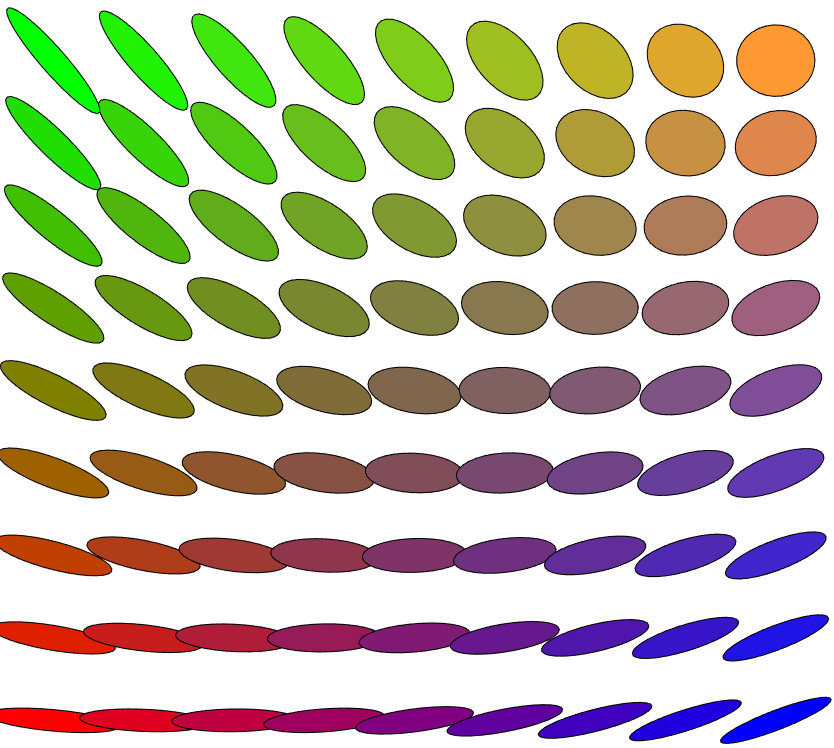
\includegraphics[width=.3\linewidth]{barycenters-gaussians/tensor-interp-70} &
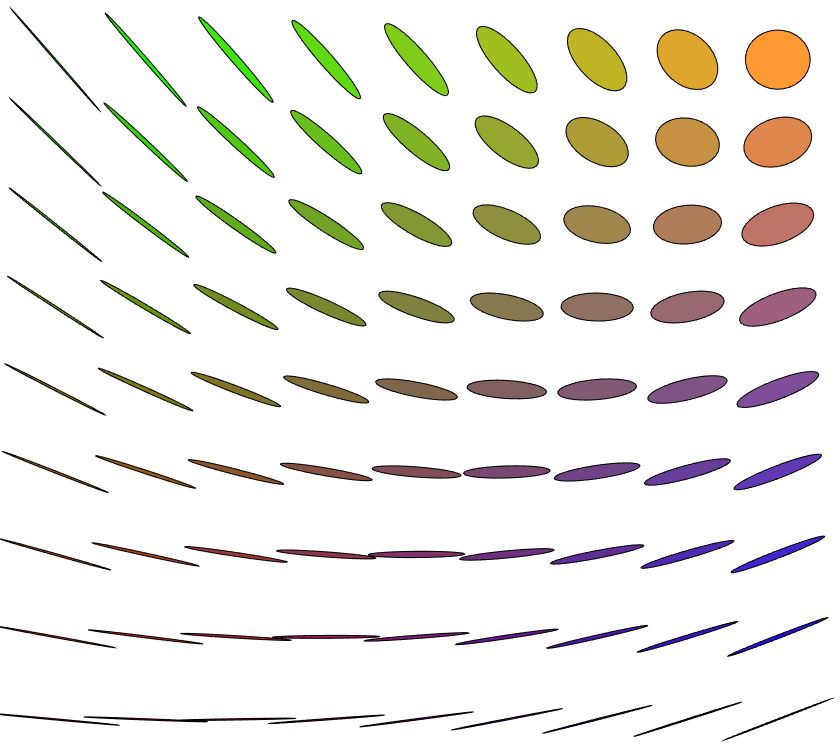
\includegraphics[width=.3\linewidth]{barycenters-gaussians/tensor-interp-98}
\end{tabular}
\caption{\label{fig-bary-gaussian}
四つの二次元ガウス分布間の重心。各ガウス分布は共分散の主軸に沿った楕円として表示され、対応する固有値に比例した伸長を持つ。
}
\end{figure}


%%%%%%%%%%%%%%%%%%%%
\begin{rem1}{一次元の場合}\label{rem-bary-1d}
	一次元分布に対して、$\Wass_p$重心は注~\ref{rem-1d-ot-generic}で詳述されているように、輸送が単調再配置であるという事実を用いてほぼ閉じた形で計算できる。
	%
	最も単純な場合は$n$点の経験測度、すなわち$\be_s = \frac{1}{n}\sum_{i=1}^n \de_{y_{s,i}}$であり、点はソート済み$y_{s,1} \leq y_{s,2} \leq \ldots$と仮定する。~\eqref{eq-1d-empirical}を用いると重心$\al_\la$も$n$点上の経験測度となる
	\eq{
		\al_\la = \frac{1}{n}\sum_{i=1}^n \de_{x_{\la,i}}
		\qwhereq
		x_{\la,i} = A_\la(x_{s,i})_s,
	}
	ここで$A_\la$は重心写像
	\eq{
	 	A_\la(x_s)_s \eqdef \uargmin{x \in \RR} \sum_{s=1}^S \la_s |x-x_{s}|^p.
	}
	である。例えば$p=2$では$x_{\la,i} = \sum_{s=1}^S \la_s x_{s,i}$となる。
	%
	一般の場合、~\eqref{eq-cumul-defn}で定義された累積関数を用いる必要があり、~\eqref{eq-wass-cumul}を用いると
	\eq{
		\foralls r \in [0,1], \quad
		\cumul{\al_\la}^{-1}(r) = A_\la( \cumul{\al_s}^{-1}(r) )_{s=1}^S,
	}
	が得られる。これは例えば、単純なソート手続きを用いて$O(n\log(n))$回の演算で$n$点未満に台を持つ離散測度間の重心を計算するために使用できる。
\end{rem1}
%%%%%%%%%%%%%%%%%%%%



%%%%%%%%%%%%%%%%%%%%
\begin{rem1}{単純な場合}
	$\T_{r,u} : x \mapsto rx+u$をスケーリングと平行移動とし、$\al_{s} = T_{r_s,u_s,\sharp} \al_0$が初期テンプレート測度をスケーリングおよび平行移動することで得られると仮定すると、重心$\al_\la$もスケーリングと平行移動により得られる\todoK{to check}
	\eq{
		\al_\la = T_{r^\star,u^\star,\sharp} \al_0
		\qwhereq
		\choice{
			r^\star = (\sum_s \la_s/r_s)^{-1},  \\
			u^\star = \sum_s \la_s u_s.
		}
	}
\end{rem1}
%%%%%%%%%%%%%%%%%%%%


%%%%%%%%%%%%%%%%%%%%
\begin{rem1}{$S=2$の場合}
	$\X=\RR^d$かつ$c(x,y)=\norm{x-y}^2$の場合（これはより一般に測地空間に拡張できる）、$S=2$つの測度$(\al_0,\al_1)$の間の重心は既に~\eqref{eq-mc-cann-interp}で導入されたマキャン補間である。$\T_\sharp \al_0=\al_1$をモンジュ写像とすると、重心$\al_\la$は$\al_\la = (\la_1 \Id + \la_2 \T)_{\sharp} \al_0$と書ける。
	%
	式~\eqref{eq-mccann-discrete}は離散の場合の計算方法を説明している。
\end{rem1}
%%%%%%%%%%%%%%%%%%%%



%%%%%%%%%%%%
\paragraph{重心のエントロピー近似。}

エントロピー平滑化を用い、ある$\epsilon>0$に対して~\eqref{eq-wass-discr}の解を以下で近似できる
\eql{\label{eq-entropic-bary}
	\umin{\a \in \simplex_n} \sum_{s=1}^S \la_s \MKD_{\C_s}^\epsilon(\a,\b_s)
}
%
これは滑らかな凸最小化問題であり、勾配降下法で解くことができる~\citep{CuturiBarycenter,GramfortPC15}。代替手段として、半双対に対する降下法（典型的には準ニュートン法）を使用することもでき~\citep{2016-Cuturi-siims}、これは重心に追加の正則化を組み込む場合、例えば与えられたノルムに関するある種の滑らかさを課す場合に有用である。
%
\citet{2015-benamou-cisc}が指摘したように、より単純かつ非常に効果的なアプローチは~\eqref{eq-entropic-bary}を（重み付き）KL射影問題として書き直すことである
\eql{\label{eq-bary-entropy-couplings}
	\umin{ (\P_s)_s } \enscond{ \sum_{s} \la_s \epsilon \KLD( \P_s|\K_s ) }{
		\foralls s, \transp{\P_s}\ones_m = \b_s, \:
		\P_1\ones_1 =  \cdots = \P_S\ones_S,
	}
}
ここで$\K_s \eqdef e^{-\C_s/\epsilon}$と表記した。ここで重心$\a$はすべての結合$\P_s \in \RR^{n \times n_s}$の行周辺に暗黙的に符号化されており、$\a = \P_1\ones_1 =  \cdots = \P_S\ones_S$である。
%
\citet{2015-benamou-cisc}で詳述されているように、シンクホーン法をこの問題に一般化でき、これは反復射影にも対応する。これは\S\ref{sec-generalized}で詳述される一般化シンクホーン法の特殊な場合とも見なせる。
%
~\eqref{eq-bary-entropy-couplings}を解く最適結合$(\P_s)_s$はスケーリング形式で以下のように計算される
\eql{\label{eq-bary-opt}
	\P_s=\diag(\uD_s)\K\diag(\vD_s),
}
そしてスケーリングは以下のように逐次的に更新される
\begin{align}\label{eq-sinkhorn-bary}
	\foralls s \in \range{1,S}, \quad \itt{\vD}_s &\eqdef \frac{\b_s}{\transp{\K}_s \it{\uD}_s}, \\
	\foralls s \in \range{1,S}, \quad  \itt{\uD}_s &\eqdef \frac{\itt{\a}}{\K_s \itt{\vD}_s}, \label{eq-sinkhorn-bary-2}\\
		\qwhereq
		\itt{\a} &\eqdef \prod_s (  \K_s \itt{\vD}_s )^{\la_s}. \label{eq-sinkhorn-bary-3}
\end{align}
これらの反復を導出する別の方法は、双対問題の変数に対して交互最小化を行うことであり、以下の命題で詳述される。

\begin{prop}
	~\eqref{eq-bary-opt}に現れる最適な$(\uD_s,\vD_s)$は$(\uD_s,\vD_s) = ( e^{\fD_s/\epsilon},e^{\gD_s/\epsilon} )$と書ける。ここで$( \fD_s,\gD_s )_s$は以下の計画の解である（その値は\eqref{eq-entropic-bary}の値と一致する）：
	\eql{\label{eq-dual-bary-entropy}
		\umax{ ( \fD_s,\gD_s )_s } \enscond{
		\sum_s \la_s \pa{
			\dotp{\gD_s}{\b_s} - \epsilon \dotp{\K_s e^{\gD_s/\epsilon}}{e^{\fD_s/\epsilon}}
		}
		}{
			\sum_s \la_s \fD_s = 0
		}.
	}
\end{prop}

\begin{proof}	~\eqref{eq-bary-entropy-couplings}にラグランジュ乗数を導入すると
	\begin{align*}
		\umin{ (\P_s)_s, \a }
		\umax{ ( \fD_s,\gD_s )_s }
		\sum_{s} \la_s \Big(
			\epsilon \KLD( \P_s|\K_s )
			+
			\dotp{\a - \P_s\ones_m}{ \fD_s } \\
		\qquad\qquad	+
			\dotp{\b_s - \transp{\P_s}\ones_m}{ \gD_s }
		\Big).
	\end{align*}
	が得られる。強双対性が成り立つため、最小と最大を交換でき、以下が得られる
		\begin{align*}
		&\umax{ ( \fD_s,\gD_s )_s }
			\sum_s \la_s \pa{
				 \dotp{\gD_s}{\b_s}
		+
		\umin{\P_s} \epsilon \KLD( \P_s|\K_s ) - \dotp{\P_s}{\fD_s \oplus \gD_s }
		} \\
	&\qquad\qquad	+ \umin{\a}
			\dotp{ \sum_{s} \la_s \fD_s }{\a}.
	\end{align*}
	$\a$に関する陽な最小化により制約$\sum_{s} \la_s \fD_s=0$が得られ、
	\begin{align*}
		\umax{ ( \fD_s,\gD_s )_s }
			\sum_s \la_s
				 \dotp{\gD_s}{\b_s}
		-
		\epsilon \KLD^*\pa{ \frac{\fD_s \oplus \gD_s}{\epsilon}|\K_s },
	\end{align*}
	となる。ここで$\KLD^*(\cdot|\K_s)$は関数$\KLD^*(\cdot|\K_s)$のルジャンドル変換~\eqref{eq-legendre}である。
	%
	このルジャンドル変換は以下のように書ける
	\eql{\label{eq-legendre-kl}
		\KLD^*(\VectMode{U}|\K) = \sum_{i,j} \K_{i,j} (e^{\VectMode{U}_{i,j}}-1),
	}
	これにより所望の公式が示される。
	%
	~\eqref{eq-legendre-kl}を示すために、この関数は分離可能であるから、以下を計算する必要がある
	\eq{
		\foralls (u,k) \in \RR_+^2, \quad
		\KLD^*(u|k) \eqdef \umax{r} ur -   \pa{ r \log(r/k) - r + k  }
	}
	その最適性条件は$u=\log(r/k)$、すなわち$r = k e^{u}$と読め、結果が得られる。
\end{proof}

すべての他の変数を固定して各$\gD_s$に関して~\eqref{eq-dual-bary-entropy}を最小化することは、~\eqref{eq-sinkhorn-bary}により閉じた形で得られる。
%
すべての$(\fD_s)_s$に関して~\eqref{eq-dual-bary-entropy}を最小化するには、~\eqref{eq-sinkhorn-bary-3}を用いて$\a$を解く必要があり、式~\eqref{eq-sinkhorn-bary-2}が導かれる。



図~\ref{fig-barycenters-images}および図~\ref{fig-barycenters-shapes}は二次元および三次元形状の補間への応用を示している。図~\ref{fig-barycenters-surfaces}は曲面上での重心の計算を示しており、グラウンドコストは測地距離の二乗である。この図では、注~\ref{rem-geod-heat}で詳述される熱の測地線近似を用いて計算が行われている。コンピュータグラフィックスおよび画像科学へのさらなる詳細と他の応用については~\citep{2015-solomon-siggraph}を参照されたい。

%
\newcommand{\FigBaryImA}[2]{\includegraphics[width=.088\linewidth]{barycenters-2d/annulus-cross-heart-2disk/shape-#1-#2}}
\newcommand{\FigBaryImLineA}[1]{\FigBaryImA{#1}{1} & \FigBaryImA{#1}{2} & \FigBaryImA{#1}{3} & \FigBaryImA{#1}{4} & \FigBaryImA{#1}{5}}
\newcommand{\FigBaryImB}[2]{\includegraphics[width=.088\linewidth]{barycenters-2d/cat-star8-thinspiral-trefle/shape-#1-#2}}
\newcommand{\FigBaryImLineB}[1]{\FigBaryImB{#1}{1} & \FigBaryImB{#1}{2} & \FigBaryImB{#1}{3} & \FigBaryImB{#1}{4} & \FigBaryImB{#1}{5}}


\begin{figure}[h!]
\centering
\fbox{
\begin{tabular}{@{}c@{}c@{}c@{}c@{}c@{}}
\FigBaryImLineA{1} \\
\FigBaryImLineA{2} \\
\FigBaryImLineA{3} \\
\FigBaryImLineA{4} \\
\FigBaryImLineA{5}
\end{tabular}
}
\fbox{
\begin{tabular}{@{}c@{}c@{}c@{}c@{}c@{}}
\FigBaryImLineB{1} \\
\FigBaryImLineB{2} \\
\FigBaryImLineB{3} \\
\FigBaryImLineB{4} \\
\FigBaryImLineB{5}
\end{tabular}
}
\caption{\label{fig-barycenters-images}
エントロピー正則化~\eqref{eq-entropic-bary}を用いた四つの入力二次元形状間の重心。バイナリ形状を表示するために、表示される画像は閾値処理された密度を示す。
%
重み$(\la_s)_s$は正方形の四隅に関して双線形である。
}
\end{figure}



% trim=left bottom right height
\newcommand{\FigBaryShapeA}[2]{\includegraphics[width=.09\linewidth,trim=130 78 110 60,clip]{barycenters-shapes/duck-spiky-moomoo_s0-double-torus/barycenter-#1-#2}}
\newcommand{\FigBaryShapeLineA}[1]{\FigBaryShapeA{#1}{0} & \FigBaryShapeA{#1}{1} & \FigBaryShapeA{#1}{2} & \FigBaryShapeA{#1}{3} & \FigBaryShapeA{#1}{4}}
%
\newcommand{\FigBaryShapeB}[2]{\includegraphics[width=.087\linewidth,trim=160 65 150 55,clip]{barycenters-shapes/mushroom-torus-hand1-trim-star/barycenter-#1-#2}}
\newcommand{\FigBaryShapeLineB}[1]{\FigBaryShapeB{#1}{0} & \FigBaryShapeB{#1}{1} & \FigBaryShapeB{#1}{2} & \FigBaryShapeB{#1}{3} & \FigBaryShapeB{#1}{4}}

\begin{figure}[h!]
\centering
%%% VOLUMETRIC SHAPES %%%
\fbox{
\begin{tabular}{@{}c@{}c@{}c@{}c@{}c@{}}
\FigBaryShapeLineA{0} \\
\FigBaryShapeLineA{1} \\
\FigBaryShapeLineA{2} \\
\FigBaryShapeLineA{3} \\
\FigBaryShapeLineA{4}
\end{tabular}
}
\fbox{
\begin{tabular}{@{}c@{}c@{}c@{}c@{}c@{}}
\FigBaryShapeLineB{0} \\
\FigBaryShapeLineB{1} \\
\FigBaryShapeLineB{2} \\
\FigBaryShapeLineB{3} \\
\FigBaryShapeLineB{4}
\end{tabular}
}
\caption{\label{fig-barycenters-shapes}
エントロピー正則化~\eqref{eq-entropic-bary}を用いた四つの入力三次元形状間の重心。重み$(\la_s)_s$は正方形の四隅に関して双線形である。
%
形状は、形状の境界内では一様で外では零であるような測度として表現される。
}
\end{figure}
ワッサーシュタイン重心の効率的な計算は、現時点でなお活発な研究テーマである~\citep{NIPS2017_6858,NIPS2018_8274}。方法論的な関心を超えて、ワッサーシュタイン重心は形状解析の分野以外でも多くの応用が見出されている。画像処理~\citep{rabin-ssvm-11}、特に色変換~\citep{2015-solomon-siggraph}（図~\ref{fig-colors}参照）；測度を要約するためのベイズ計算~\citep{srivastava2015scalable,srivastava2015wasp}；および非線形次元削減、すなわち入力測度を他の既知の測度のワッサーシュタイン重心として表現するもの~\citep{2016-bonneel-barycoord}に使用されている。これらの問題はすべて、自動微分（注~\ref{rem-auto-diff}参照）を用いて正確に最適化できる複雑な非凸目的関数をもたらす。
%
重心の計算に密接に関連する問題には、ワッサーシュタイン空間上の主成分分析の計算（例えば~\citep{SeguyCuturi,bigot2017geodesic}を参照）およびテンプレートモデルの統計的推定~\citep{boissard2015distribution}がある。重心を計算する能力は、確率測度の空間上の$k$平均法~\citep{del2016robust,ho2017multilevel}のようなより高度なクラスタリング手法を可能にする。




\begin{figure}[h!]
\centering
\begin{tabular}{@{}c@{}c@{}c@{}c@{}c@{}}
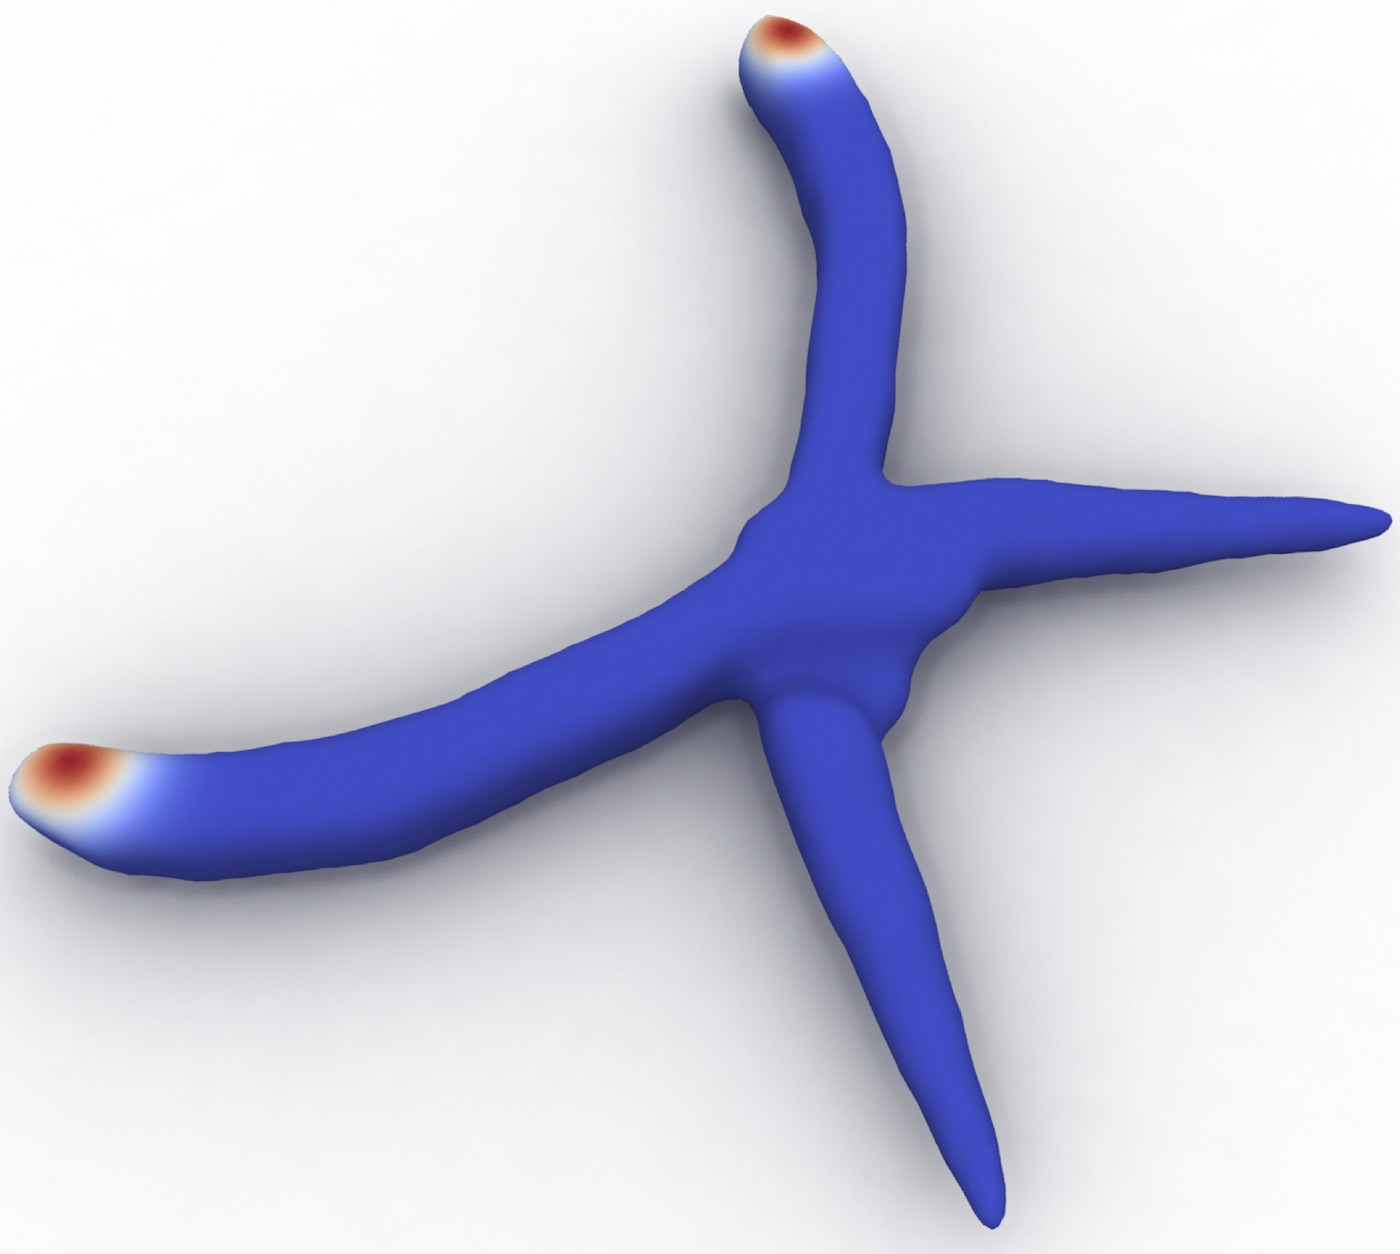
\includegraphics[width=.195\linewidth]{barycenters-surfaces/scisor-1}&
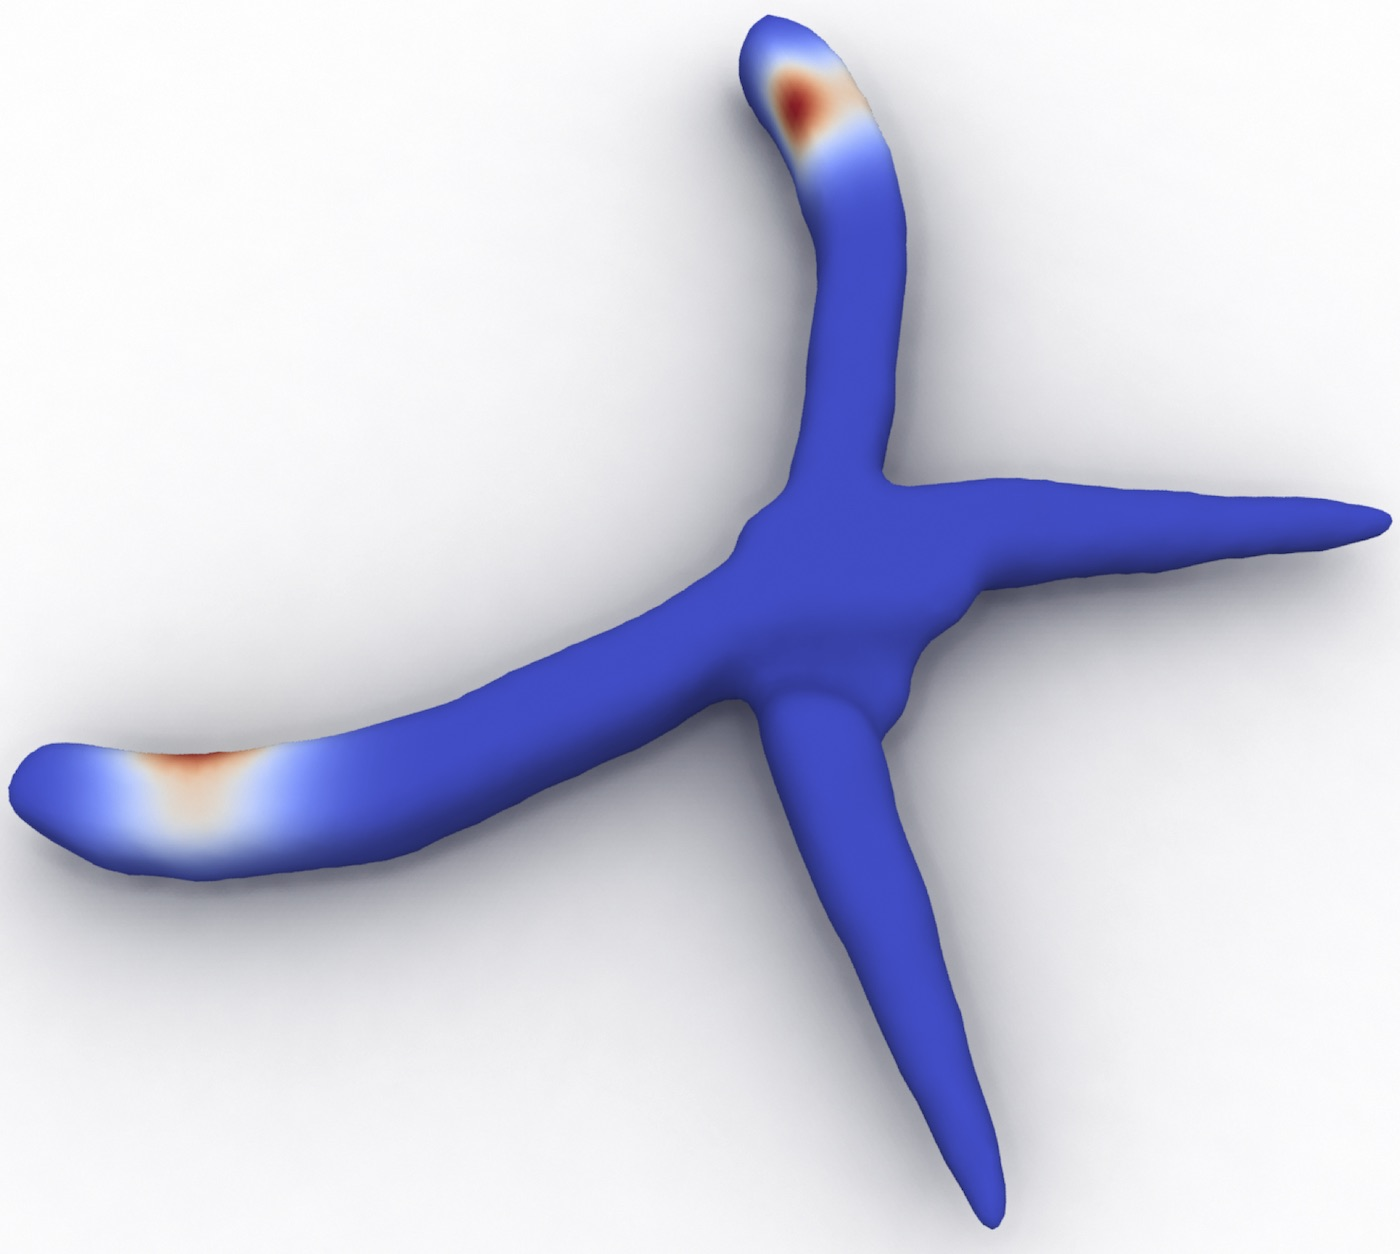
\includegraphics[width=.195\linewidth]{barycenters-surfaces/scisor-2}&
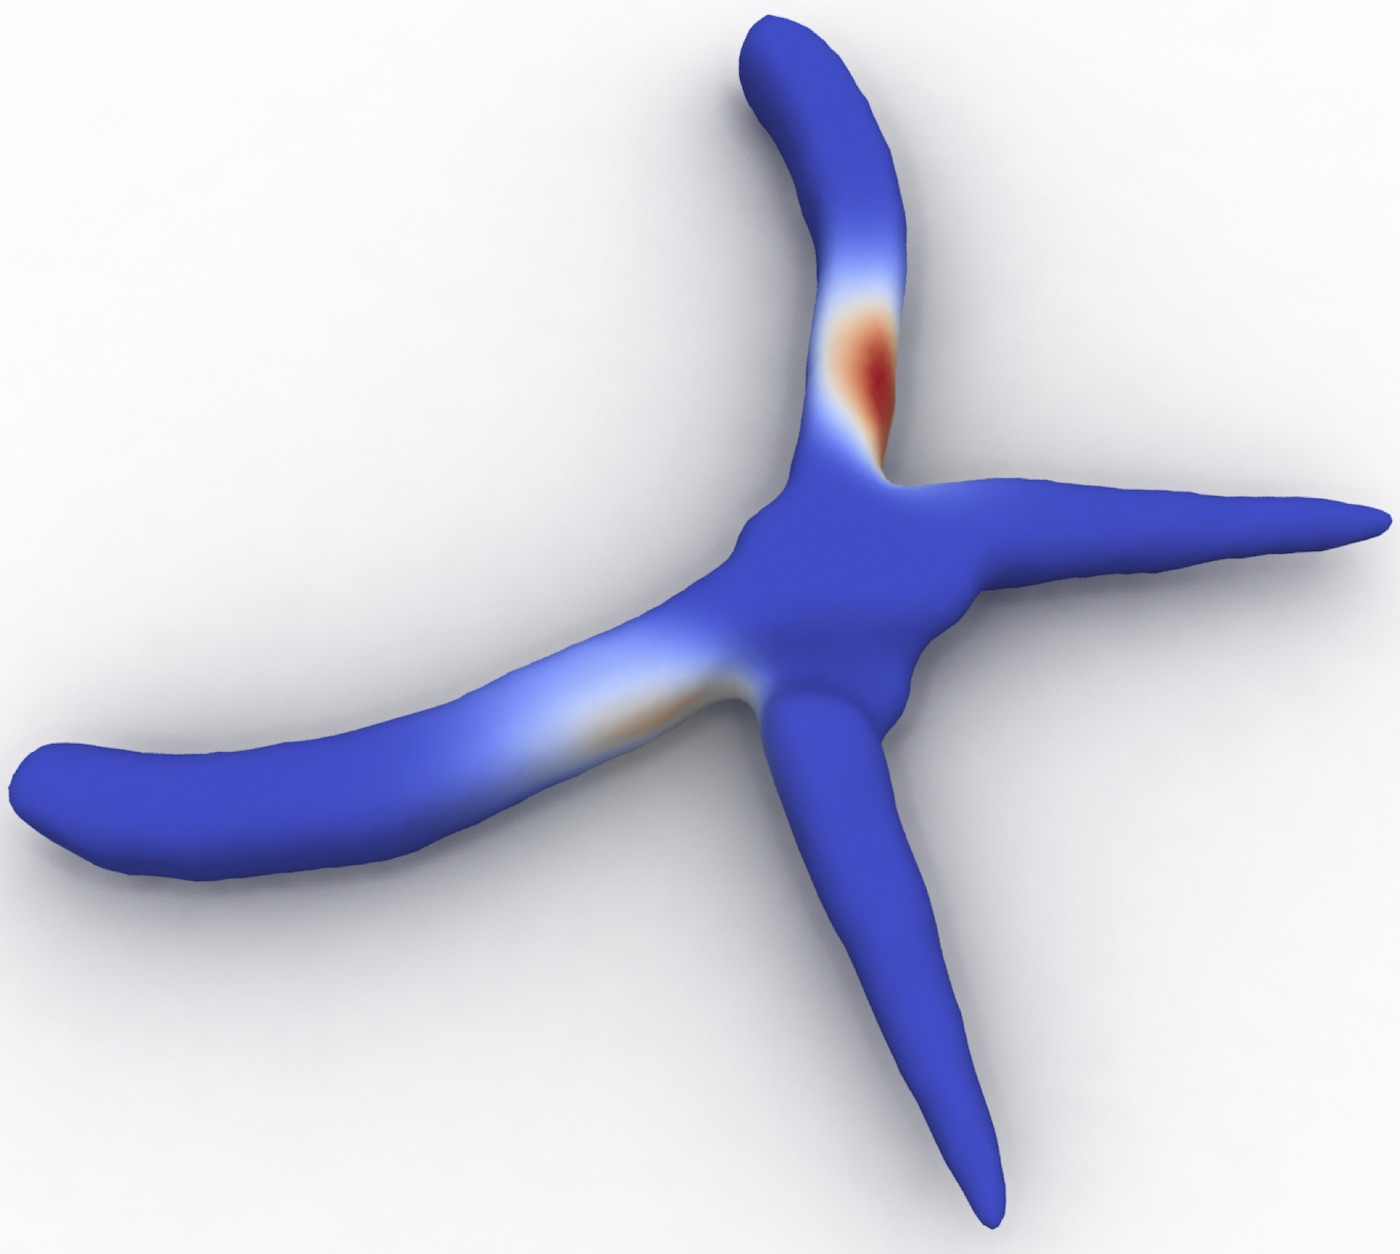
\includegraphics[width=.195\linewidth]{barycenters-surfaces/scisor-3}&
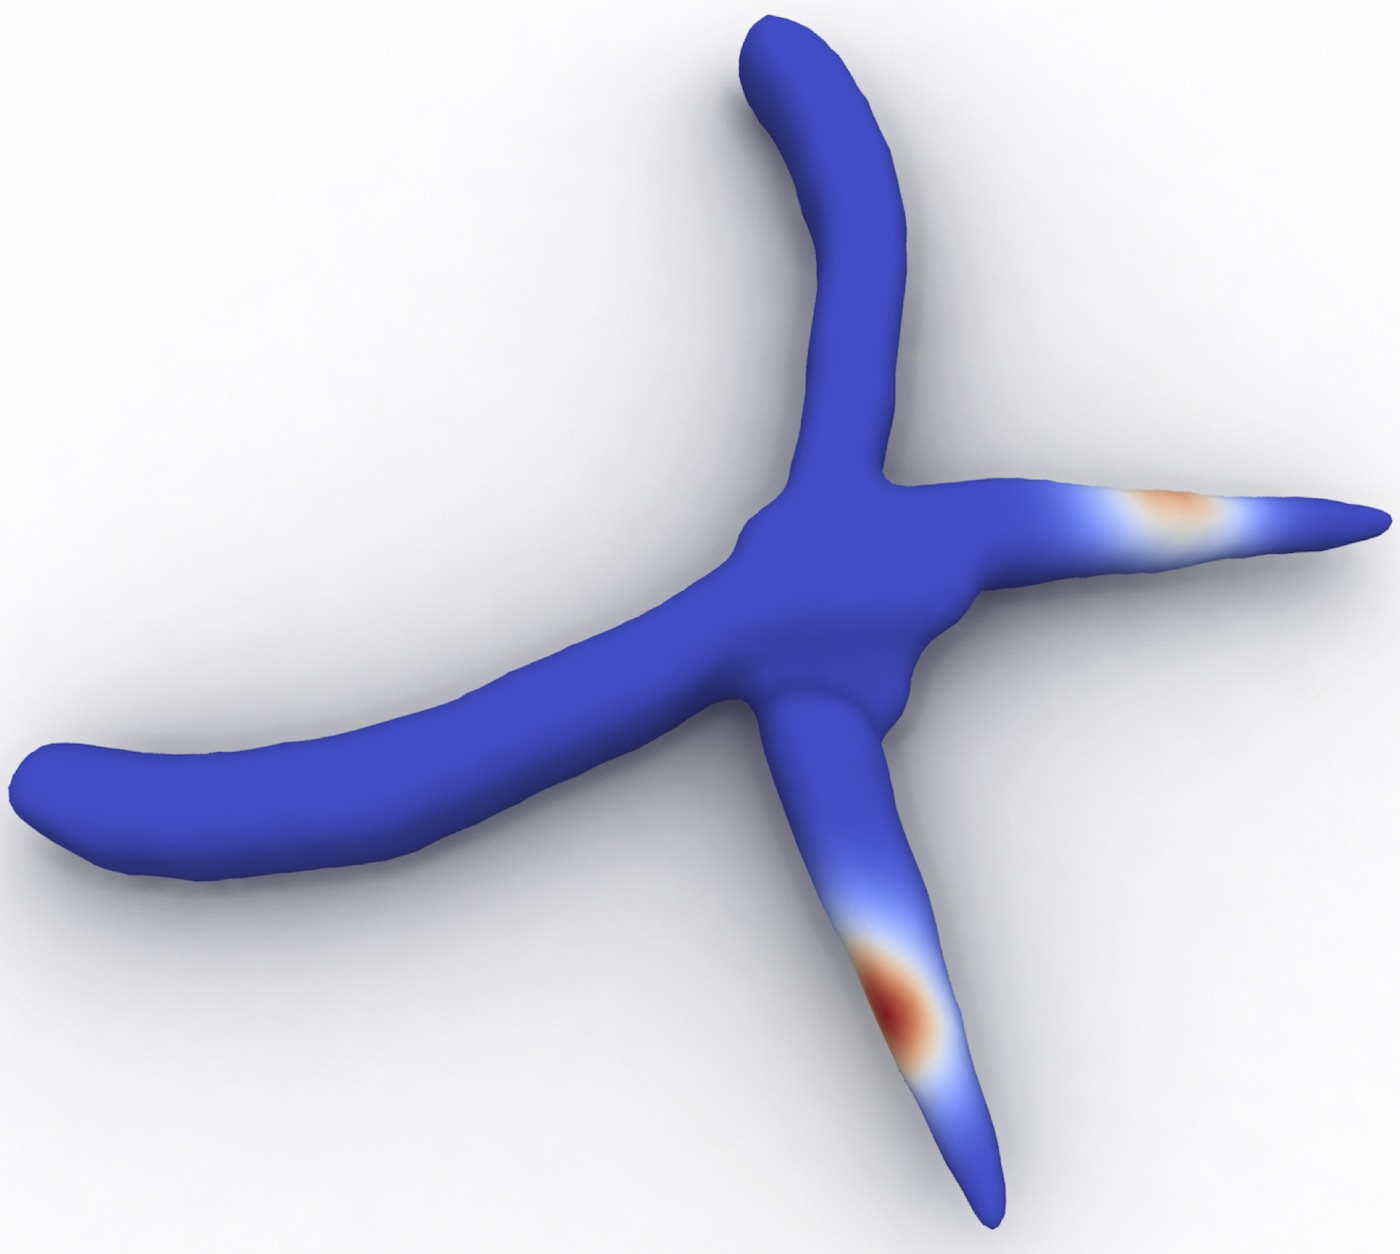
\includegraphics[width=.195\linewidth]{barycenters-surfaces/scisor-4}&
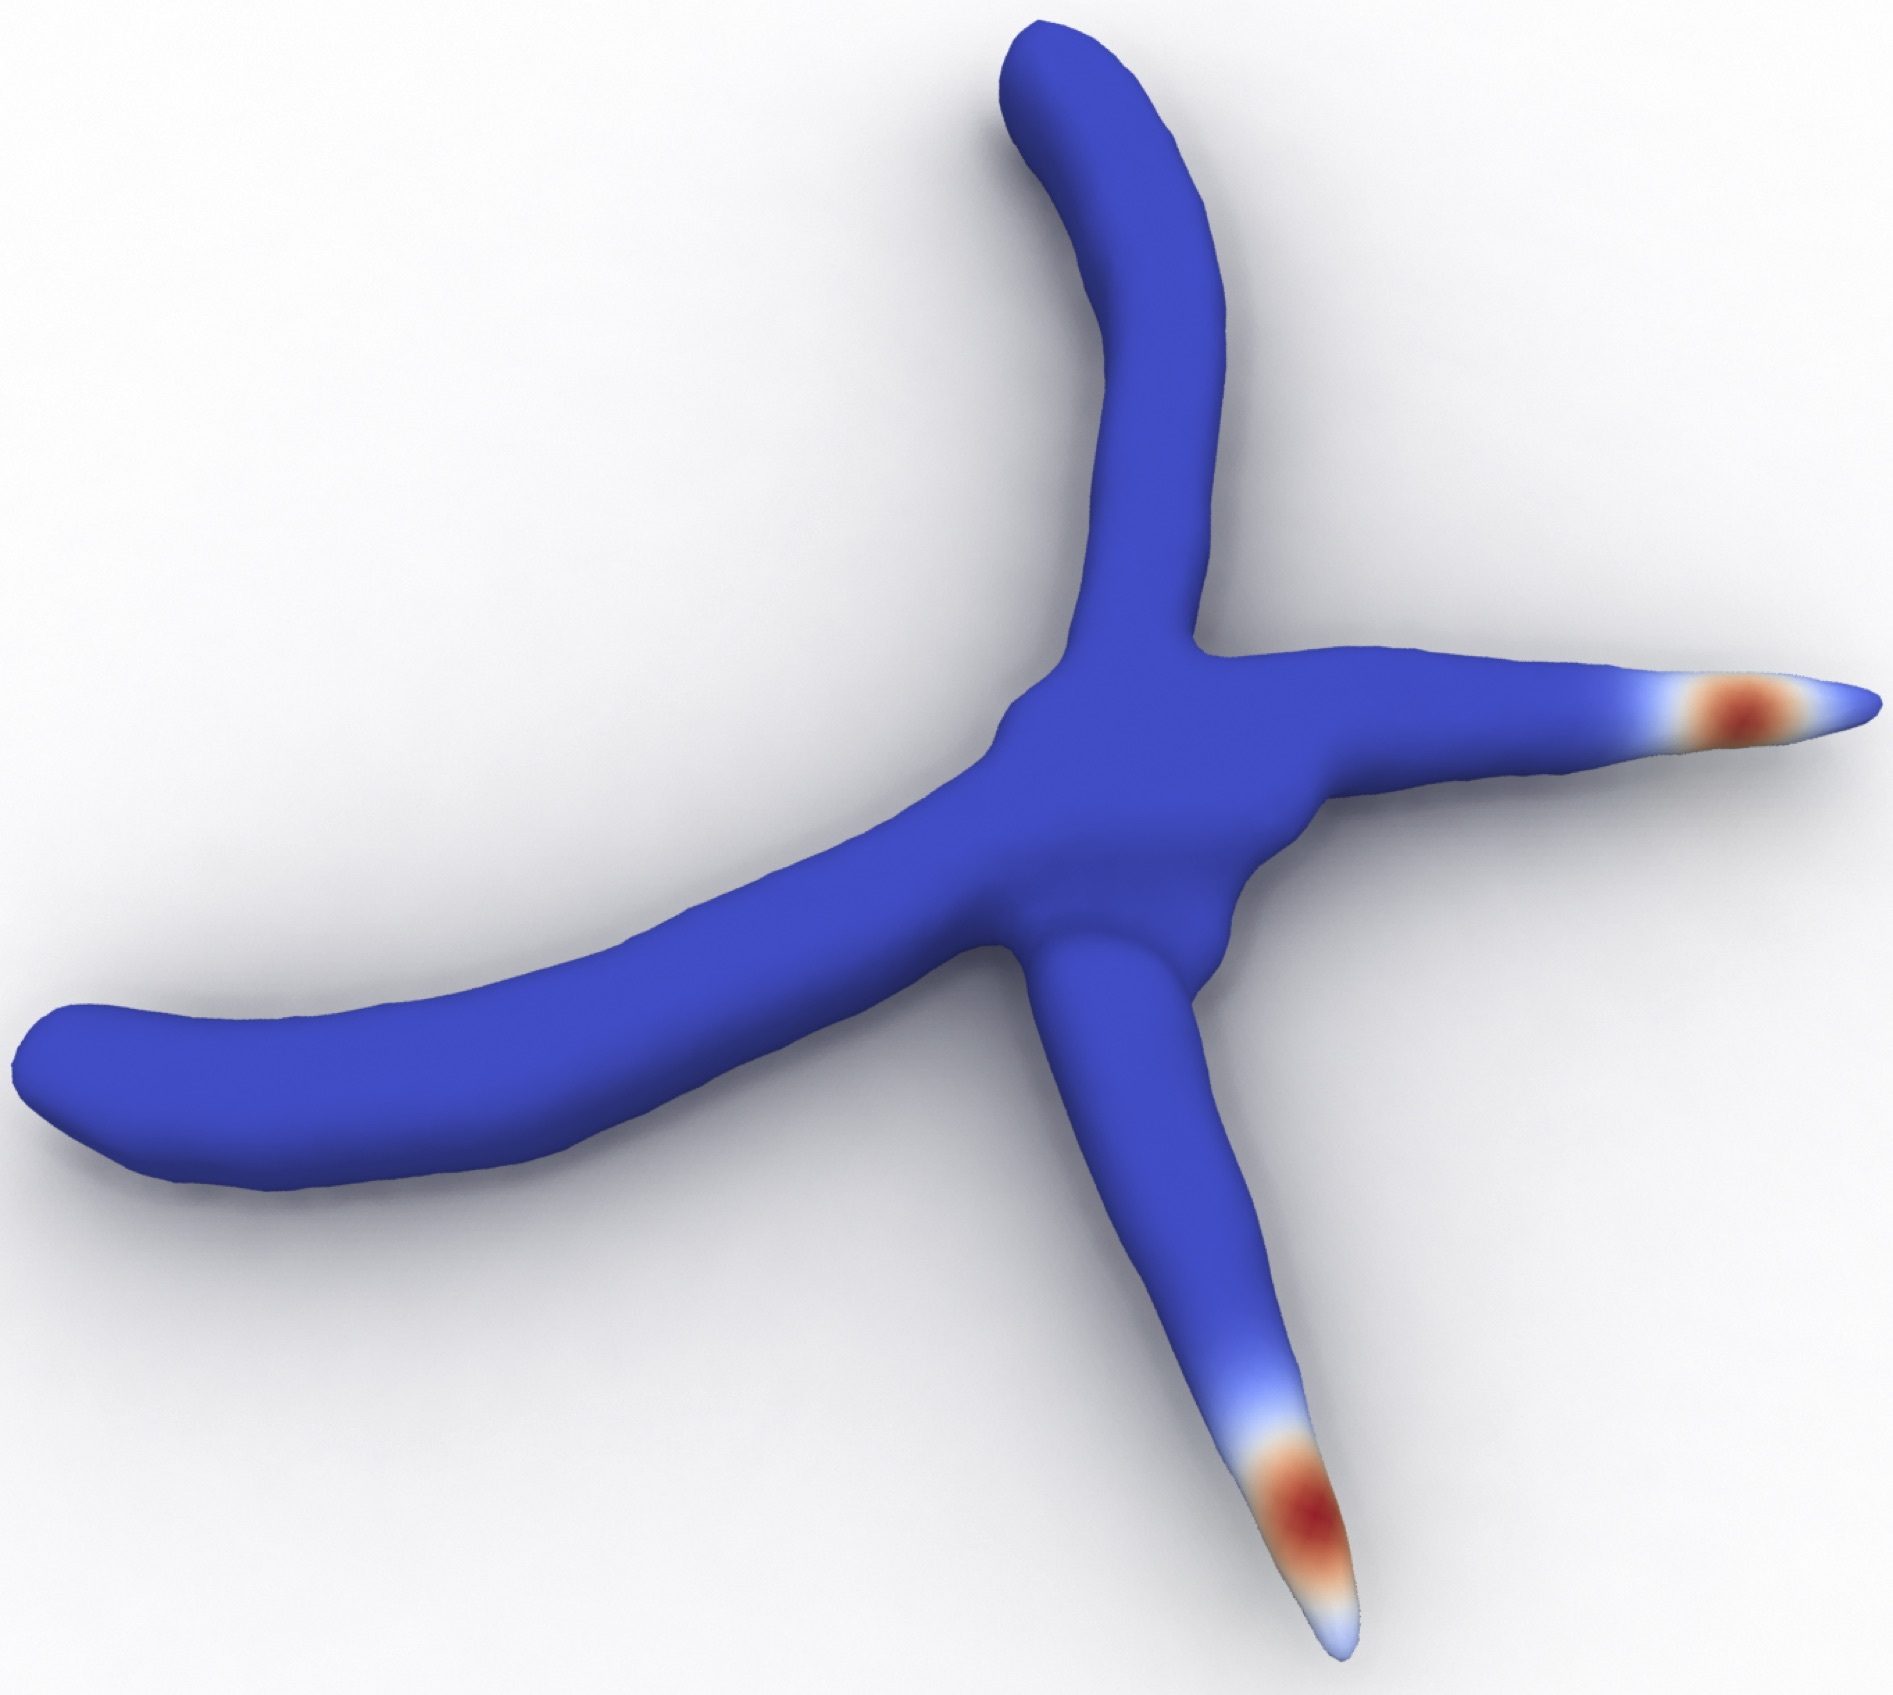
\includegraphics[width=.195\linewidth]{barycenters-surfaces/scisor-5}
\end{tabular}
\caption{\label{fig-barycenters-surfaces}
熱の測地線高速カーネル近似（注~\ref{rem-geod-heat}参照）を用いて計算された、曲面上の二つの入力測度間の重心補間。~\citep{2015-solomon-siggraph}より抜粋。
}
\end{figure}



\begin{figure}[h!]
\centering
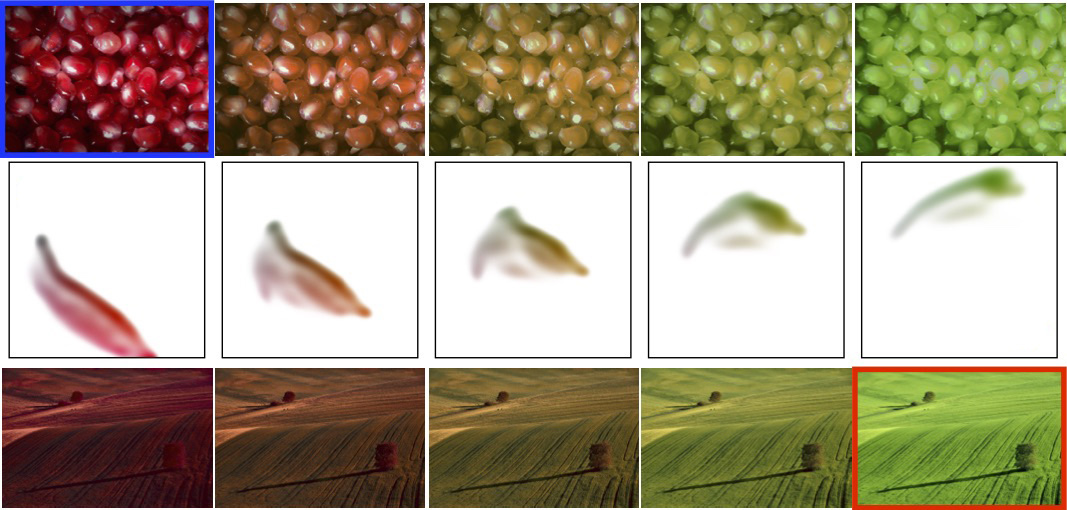
\includegraphics[width=1\linewidth]{colors/colors-bary}
\caption{\label{fig-colors}
二つの入力画像の二つの三次元色経験ヒストグラム間の補間（ここでは簡単のため二次元色度射影のみが可視化されている）。変更されたヒストグラムは注~\ref{rem-barycenric-proj}で詳述される重心射影を用いて入力画像に適用される。~\citep{2015-solomon-siggraph}より抜粋。
}
\end{figure}



%%%%%%%%%%%%%%%%%%%%
\begin{rem1}{ワッサーシュタイン伝播}
	\citet{Solomon-ICML}で研究されているように、重心問題~\eqref{eq-wass-discr}を一般化することが可能である。ここではグラフ$\Gg$内の与えられたノード集合$U$上の分布$(\b_u)_{u \in U}$を、ノードの補集合$V$上の固定された入力分布$(\b_v)_{v \in V}$が与えられたもとで求める。未知量は、グラフのエッジを形成するすべてのノード対$(r,s) \in \Gg$間の総輸送距離を最小化することにより決定される
	\eql{\label{eq-w-propag}
		\umin{(\b_u  \in \simplex_{n_u})_{u \in U}}
			\sum_{(r,s) \in \Gg}  \MKD_{\C_{r,s}}(\b_r,\b_s),
	}
	ここでコスト行列$\C_{r,s} \in \RR^{n_r \times n_s}$はユーザーが指定する必要がある。
	%
	重心問題~\eqref{eq-wass-discr}はこの問題の特殊な場合であり、考慮されるグラフ$\Gg$は「星型」であり、$U$は他のすべての頂点$V$に接続された単一の頂点である（$\b_s$に付随する重み$\la_s$はコスト行列に吸収できる）。
	%
	各エッジ$(r,s) \in \Gg$に対して結合$\P_{r,s} \in \CouplingsD( \b_r,\b_s )$を陽に導入し、エントロピー正則化を用いると、~\eqref{eq-bary-entropy-couplings}と同様にこの問題を書き直すことができ、シンクホーン反復~\eqref{eq-sinkhorn-bary}をこの問題に拡張できる（これは\S\ref{sec-generalized}で詳述される一般化シンクホーンアルゴリズムの形にこの問題を再定式化することでも導出できる）。
	%
	\todoK{show a graphical illustration}
	%
	グラフ上のこの離散変分問題~\eqref{eq-w-propag}は、グラフを連続領域に置き換えた場合にディリクレエネルギーを定義するように一般化できる~\citep{solomon2013dirichlet}。これにより測度値調和関数の定義が導かれ、画像および曲面処理への応用が見出される。理論的解析については~\citet{Lavenant2017}、非二次的（全変動）汎関数への拡張と画像処理への応用については~\citet{vogt2017measure}も参照されたい。
\end{rem1}
%%%%%%%%%%%%%%%%%%%%



%%%%%%%%%%%%%%%%%%%%%%%%%%%%%%%%%%%%%%%%%%%%%%%%%%%%%%%%%%%%%%%%%%%%%%%%%%
%%%%%%%%%%%%%%%%%%%%%%%%%%%%%%%%%%%%%%%%%%%%%%%%%%%%%%%%%%%%%%%%%%%%%%%%%%
%%%%%%%%%%%%%%%%%%%%%%%%%%%%%%%%%%%%%%%%%%%%%%%%%%%%%%%%%%%%%%%%%%%%%%%%%%
\section{勾配流}
\label{sec-grad-flows}

滑らかな関数$\a \mapsto F(\a)$が与えられたとき、標準的な勾配降下法
\eql{\label{eq-explicit-euclidean}
	\itt{\a} \eqdef \it{\a} - \tau \nabla F(\it{\a}),
}
を使用できる。ここで$\tau$は十分小さなステップサイズである。これはいわゆる「陽的」最小化スキームに対応し、滑らかな関数$F$にのみ適用される。非滑らかな関数に対しては、代わりに「陰的」スキームを使用でき、これは近接点アルゴリズムとも呼ばれる（例えば~\citet{BauschkeCombettes11}参照）
\eql{\label{eq-implicit-euclidean}
	\itt{\a} \eqdef \Prox_{\tau F}^{\norm{\cdot}}(\it{\a}) \eqdef \uargmin{\a} \frac{1}{2}\norm{\a-\it{\a}}^2 + \tau F(\a).
}
これは~\eqref{eq-prox-eucl}で既に遭遇したユークリッド近接作用素に対応することに注意する。
%
更新~\eqref{eq-explicit-euclidean}は陽的作用素$\Id-\tau\nabla F$の反復と理解でき、一方~\eqref{eq-implicit-euclidean}は陰的作用素$(\Id+\tau\nabla F)^{-1}$を使用する。凸な$F$に対しては、反復~\eqref{eq-implicit-euclidean}は$\tau>0$のいかなる値に対しても常に収束する。

関数$F$がヒストグラムのシンプレックス$\simplex_n$上で定義されている場合、~\eqref{eq-implicit-euclidean}の$\ell^2$ノルム$\norm{\cdot}$の代わりに最適輸送距離を使用することが理にかなっており、以下を解くことになる
\eql{\label{eq-grad-flow-discr}
	\itt{\a} \eqdef \uargmin{\a} \WassD_p(\a,\it{\a})^p + \tau F(\a).
}

%%%%%%%%%%%%%%%%%%
\begin{rem2}{ワッサーシュタイン勾配流}
式~\eqref{eq-grad-flow-discr}は、反復
\eql{\label{eq-grad-flow-stepping-cont}
	\itt{\al} \eqdef \uargmin{\al} \Wass_p(\al,\it{\al})^p + \tau F(\al)
}
を定義することで任意の測度に一般化でき、ここで$F$は$\Mm_+^1(\X)$上で定義されたある関数である。この陰的時間ステッピングは連続流を構成するための有用なツールであり、形式的に極限$\tau \rightarrow 0$をとり時間$t=\tau \ell$を導入することで、$\it{\al}$は連続流$t \in \RR_+ \mapsto \al_t$を近似することを意図している。$p=2$かつ$\X=\RR^d$の特殊な場合には、形式的な計算により$\al_t$は以下の形のPDEを解くことが期待される
\eql{\label{eq-grad-flow-cont}
	\pd{\al_t}{t} = \diverg( \al_t \nabla( F'(\al_t) ) ),
}
ここで$F'(\al)$は連続関数$F'(\al) \in \Cc(\X)$であるという意味での関数$F$の微分であり、
\eq{
	F(\al+\epsilon\xi) = F(\al) + \epsilon \int_\X F'(\al) \d\xi(x) + o(\epsilon).
}
を満たす。典型的な例は$F=-\H$を用いる場合であり、ここで$\H(\al)=\KL(\al|\Ll_{\RR^d})$は$\X=\RR^\dim$上のルベーグ測度$\Ll_{\RR^d}$に関する相対エントロピーである
\eql{\label{eq-entropy-cont}
	\H(\al) = - \int_{\RR^\dim} \density{\al}(x) (\log(\density{\al}(x)) - 1) \d x
}
（$\al$が密度を持たないとき$\H(\al)=-\infty$と設定する）。このとき~\eqref{eq-grad-flow-cont}により、この負エントロピーの勾配流は線形熱拡散
\eql{\label{eq-heat}
	\pd{\al_t}{t} = \Delta \al_t,
}
であることが示される。ここで$\Delta$は空間ラプラシアンである。
%
したがって、熱拡散はディリクレエネルギー$\int_{\RR^\dim} \|\nabla \density{\al}(x)\|^2 \d x$の「古典的な」ユークリッド流（ある意味で質量振幅に関する「垂直的」移動を行う）として、あるいは代替的に最適輸送流に対するエントロピー（ある意味で質量位置に関する「水平的」移動）として解釈できる。
%
ワッサーシュタイン勾配流への関心は、Jordan、KinderlehrerおよびOttoの画期的な論文~\citep{jordan1998variational}により喚起され、これらの発展はしばしば彼らの研究にちなんで「JKO流」と呼ばれる。\citet{ambrosio2006gradient}による専門書で詳述されているように、JKO流は距離空間における勾配流の特殊な場合である。最近のサーベイ論文~\citep{santambrogio2017euclidean}も参照されたい。
%
JKO流は特に多孔質媒体方程式~\citep{otto2001geometry}、全変動流~\citep{carlier2017total}、量子ドリフト~\citep{GianazzaARMA}、または多様体上の熱発展~\citep{ErbarHeatManifold}などの非線形発展方程式の研究に使用できる。その柔軟な形式は解に対する制約を許容し、例えば密度の上限である混雑制約を\citeauthor{maury2010macroscopic}が群衆運動のモデル化に使用した~\citep{maury2010macroscopic}（レビュー論文~\citep{SantambrogioCrowdReview}も参照）。
\end{rem2}
%%%%%%%%%%%%%%%%%%%


%%%%%%%%%%%%%%%%%%
\begin{rem2}{距離空間における勾配流}
陰的ステッピング~\eqref{eq-grad-flow-stepping-cont}は、~\citep{ambrosio2006gradient}で詳述されているように、距離空間$(\Xx,\dist)$（$\dist$は距離）上で勾配流を定義するためのより一般的な形式の特殊な場合である。
%
$x \in \Xx$に対して定義されたある関数$F(x)$に対して、陰的離散最小化ステップは以下のように定義される
\eql{\label{eq-implicit-metricflow}
	\itt{x} \in \uargmin{x \in \Xx} \dist(\it{x},x)^2 + \tau F(x).
}
JKOステップ~\eqref{eq-grad-flow-stepping-cont}は確率分布の空間上でワッサーシュタイン距離を使用する場合に対応する。場合によっては、~\eqref{eq-implicit-metricflow}は$\tau \rightarrow 0$かつ$k\tau=t$のとき連続流の極限$x_t$を持つことが示せる。
%
$\Xx$がユークリッド構造も持つ場合、$F$を線形化することで陽的ステッピングが定義される
\eql{\label{eq-explicit-metricflow}
	\itt{x} = \uargmin{x \in \Xx} \dist(\it{x},x)^2 + \tau \dotp{ \nabla F(\it{x}) }{ x }.
}
陰的公式~\eqref{eq-implicit-metricflow}とは対照的に、これは通常計算が直截的であるが不安定になりうる。陰的ステップは常に安定であり、非滑らかな$F$に対しても定義されるが、通常閉じた形では得られない。
%
図~\ref{fig-gradflow-metric}は関数$F(x) = \norm{x}^2$を$\Xx=\RR^2$上で、距離$d(x,y)=\norm{x-y}_p=(|x_1-y_1|^p+|x_2-y_2|^p)^{\frac{1}{p}}$に対して$p$のいくつかの値で示したこの概念を図解している。
%
陽的スキーム~\eqref{eq-explicit-metricflow}は$p=1$と$p=+\infty$で不安定であり、$p=1$では軸に沿ったステップ（座標ごとの降下）を与える。
%
対照的に、陰的スキーム~\eqref{eq-implicit-metricflow}は安定である。特に$p=1$の場合、二つの座標が等しいとき、次のステップが対角方向に作用することに注意されたい。
\end{rem2}
%%%%%%%%%%%%%%%%%%


\begin{figure}[h!]
\centering
\begin{tabular}{cc}

\includegraphics[width=.45\linewidth]{gradflow-metric/explicit}&

\includegraphics[width=.45\linewidth]{gradflow-metric/implicit}\\
Explicit & Implicit
\end{tabular}
\caption{\label{fig-gradflow-metric}
距離$d(x,y)=\norm{x-y}_p$に対する$p$のいくつかの値での、$\Xx=\RR^2$上の関数$f(x) = \norm{x}^2$を最小化するための陽的および陰的勾配流の比較。
}
\end{figure}


%%
\begin{rem1}{粒子系を用いたラグランジュ離散化}\label{rem-lagr-discretization}
~\eqref{eq-grad-flow-discr}の有限次元問題は、測度の空間上の流れ~\eqref{eq-grad-flow-stepping-cont}のオイラー離散化と解釈できる。
%
問題を離散化する別の方法として、いわゆる粒子系を用いたラグランジュ法では、解を代わりに時間とともに移動する（離散的な）経験測度としてパラメータ化し、その測度の位置（重みではなく）が関心のある変数となる。実際には、時間でインデックスされた粒子の動的な点群$\al_t = \frac{1}{n}\sum_{i=1}^n \de_{x_i(t)}$を考えることができる。
%
元の問題~\eqref{eq-grad-flow-discr}は、点の動力学を規定する$n$個の連立常微分方程式$X(t)=(x_i(t))_i \in \X^n$に置き換えられる。
%
エネルギー$F$が離散測度に対して有限であれば、単に$\Ff(X)=F( \frac{1}{n}\sum_{i=1}^n \de_{x_i} )$と定義できる。典型的な例は線形関数$F(\al) = \int_\X V(x) \d\al(x)$と二次相互作用$F(\al) = \int_{\X^2} W(x,y) \d\al(x)\d\al(y)$であり、この場合それぞれ
\eq{
	\Ff(X) = \frac{1}{n} \sum_i V(x_i) \qandq \Ff(X) = \frac{1}{n^2} \sum_{i,j} W(x_i,x_j).
}
を使用できる。
%
密度を持つ測度に対してのみ有限である一般化エントロピーのような関数に対しては、点群を密度に変換するための密度推定量を適用する必要があり、これにより$n \rightarrow +\infty$のとき$F$と整合的な関数$\Ff(x)$も定義できる。典型的な例は~\eqref{eq-entropy-cont}で定義されたエントロピー$F(\mu) = \H(\al)$であり、整合的な推定量（定数項を除いて）は最近傍までの距離の対数の和として得られる
\eql{\label{eq-entropy-discretized}
	\Ff(X) = \frac{1}{n}\sum_{i} \log( d_X(x_i) )
	\qwhereq d_X(x) = \umin{x' \in X, x' \neq x} \norm{x-x'};
}
ノンパラメトリックエントロピー推定量のレビューについては~\citet{beirlant1997nonparametric}を参照されたい。
%
十分小さなステップサイズ$\tau$に対して、$\X=\RR^\dim$と仮定すると、ワッサーシュタイン距離$\Wass_2$は点上のユークリッド距離と一致する。すなわち$|t-t'|$が十分小さければ$\Ww_2(\al_t,\al_{t'})=\norm{X(t)-X(t')}$である。したがって勾配流は位置に関するユークリッド流$X'(t) = -\nabla \Ff(X(t))$と等価であり、これは時刻$t_k=\tau k$に対して~\eqref{eq-explicit-euclidean}と同様に陽的オイラーステップで離散化される
\eq{
	\itt{X} \eqdef \it{X} - \tau \nabla \Ff(\it{X}).
}
%
図~\ref{fig-flow-lagr}は線形関数とエントロピー汎関数の和に対するこのような離散化された陽的発展の例を示しており、フォッカー・プランク方程式の離散化版が得られる。
%
この特殊な線形フォッカー・プランク方程式の場合、確率的PDEの方法に頼ることも可能であり、ガウスドリフトを持つ単一のランダム粒子を発展させることで数値的に近似できることに注意する。これらのスキーム（いわゆるランジュバン・モンテカルロ法）の定常分布への収束は、ワッサーシュタイン距離の観点から定量化できる。例えば~\citep{dalalyan2017user}を参照されたい。\todoK{Detailed this much more.}
%
関数$\Ff$が滑らかでない場合、~\eqref{eq-implicit-euclidean}と同様に陰的オイラーステップを用いて離散化すべきである。すなわち
\eq{
	\itt{X} \eqdef \Prox_{\tau \Ff}^{\norm{\cdot}}(\it{X}) \eqdef \uargmin{Z \in \X^n} \frac{1}{2}\norm{Z-\it{X}}^2 + \tau \Ff(Z).
}
を考える。
%
線形関数$F(\al) = \int_X V(x) \d\al(x)$の最も単純な場合、流れは各粒子$x_i(t)$に対して独立に作用し、関数$V$に対する通常のユークリッド流$x_i'(t)=-\nabla V(x_i(t))$に対応する（そして流れの積分曲線に沿った密度の移流PDEである）。
\end{rem1}

\newcommand{\FigLagrFlow}[1]{\includegraphics[width=.19\linewidth]{lagrangian-flows/lagrange-flow-#1}}


\begin{figure}[h!]
\centering
\begin{tabular}{@{}c@{}c@{}c@{}c@{}c@{}}
\FigLagrFlow{1} &
\FigLagrFlow{3} &
\FigLagrFlow{5} &
\FigLagrFlow{7} &
\FigLagrFlow{10} \\
$t=0$ & $t=0.2$  & $t=0.4$ & $t=0.6$ & $t=0.8$
\end{tabular}
\caption{\label{fig-flow-lagr}
関数$F(\al) = \int V \d\al - H(\al)$（$V(x)=\norm{x}^2$）に対するラグランジュ離散化を用いた勾配流発展の例。
%
エントロピーは~\eqref{eq-entropy-discretized}を用いて離散化されている。
%
極限定常分布はガウス分布である。
}
\end{figure}


%%%%%%%%%%%%%%%%%%
\begin{rem2}{測地的凸性}
勾配流に関連する重要な概念は、ワッサーシュタイン-2幾何学に関する汎関数$F$の凸性、すなわちワッサーシュタイン測地線（注~\ref{rem-displacement}で示される変位補間）に沿った$F$の凸性である。そのような関数に対するワッサーシュタイン勾配流（連続時間）は存在し、一意であり、$\tau \rightarrow 0$のときの離散ステッピング~\eqref{eq-grad-flow-stepping-cont}の極限である。これは$t \rightarrow +\infty$のとき固定された定常分布に収束する。
%
エントロピーは測地的凸関数の典型的な例であり、線形関数$F(\al) = \int_\X V(x) \d\al(x)$および凸関数$V : \X \rightarrow \RR$、$W : \X \times \X \rightarrow \RR$に対する二次相互作用関数$F(\al) = \int_{\X \times \X} W(x,y) \d\al(x) \d\al(y)$もそうである。
%
線形関数は古典的な意味で凸であるが、二次相互作用関数はそうでない場合があることに注意する。
%
典型的な例は$W(x,y)=\norm{x-y}^2$であり、これは負半正定核（定義~\ref{def-negativedefinitekernel}参照）であるため、$F(\al)$は通常の意味で凹な関数に対応する（一方で測地的には凸である）。
%
\citet{mccann1997convexity}の重要な結果として、$\X=\RR^\dim$上の形式$F(\al) = \int_{\RR^\dim} \phi(\density{\al}(x)) \d x$の一般化「エントロピー」関数は、$\phi$が凸であり、$\phi(0)=0$、$t \rightarrow +\infty$のとき$\phi(t)/t \rightarrow +\infty$、かつ$s \mapsto s^{\dim} \phi(s^{-\dim})$が凸減少であるならば、測地的に凸である。
\end{rem2}
%%%%%%%%%%%%%%%%%%%

結果として得られる離散化された流れの数値解法に関する重要な文献があり、ここではいくつかの代表的な出版物のみを挙げる。一次元問題に対しては、最適輸送が逆累積関数において二次汎関数であるため（注~\ref{rem-1d-ot-generic}参照）、非常に精密なソルバーが開発されている：\citet{kinderlehrer1999approximation,blanchet2008convergence,agueh2013one,Matthes1D,blanchet2012optimal}。高次元では、有限要素法および有限体積法を用いて取り組むことができる：\citet{CarrilloFiniteVolume,burger2010mixed}。代替的なソルバーはラグランジュスキーム（すなわち粒子系）を用いて得られる：\citet{carrillo2009numerical,JDB-JKO,Westdickenberg2010}。
%
もう一つの方向は、連続的な対応物の一部の性質を維持する離散流（典型的には離散グリッドまたはグラフ上）を探すことである。~\citet{MielkeCVPDE,ErbarDCDS,ChowHuangLiZhou2012,Maas2011}を参照されたい。


エントロピー正則化に基づくオイラー離散化問題~\eqref{eq-explicit-euclidean}を解くための近似的アプローチは~\citet{2015-Peyre-siims}で最初に提案され、~\citet{2016-chizat-sinkhorn}で改良され、~\citet{2017-carlier-SIMA}で理論的に解析された。
%
エントロピー正則化を用いると、問題~\eqref{eq-grad-flow-discr}は$G = \iota_{\it{\a}}$と設定し$F$を$\tau F$に置き換えたとき~\eqref{eq-generalized-ot-regul}の形になる。したがって、~\citet{2015-Peyre-siims}で最初に提案されたように、反復~\eqref{eq-gen-sinkh}を用いて$\itt{\a}$を近似できる。$\epsilon \rightarrow 0$のときのこのスキームの収束は~\citet{2017-carlier-SIMA}で証明されている。
%
図~\ref{fig-jko}はこの方法で計算された発展の例を示している。
%
勾配流の機械学習への興味深い応用は、密度のある動力学モデルを最もよくモデル化する基礎関数$F$を学習することである。この学習はエントロピー正則化された輸送と自動微分（注~\ref{rem-auto-diff}参照）を用いた滑らかな非凸最適化を解くことで達成できる。~\citet{hashimoto2016learning}を参照されたい。

時間と空間の両方で離散化された勾配流の収束を解析することは一般に困難である。距離を定義する線形計画問題の多面体的性質により、ステップサイズを小さくしすぎると「ロッキング」現象（分布が動かなくなり発展しなくなるため、ステップサイズは小さすぎてはならない、~\citep{maury201713}で議論されている）が生じる。一次元における勾配流の離散化法の収束解析については~\citep{Matthes1D,matthes2017convergent}を参照されたい。


\begin{figure}[h!]
\centering
\begin{tabular}{@{}c@{\hspace{1mm}}c@{\hspace{1mm}}c@{\hspace{1mm}}c@{\hspace{1mm}}c@{}}

\includegraphics[width=.19\linewidth]{jko/congestion/holes-potential}&
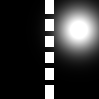
\includegraphics[width=.19\linewidth]{jko/congestion/holes-kappa10-1}&
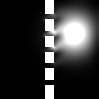
\includegraphics[width=.19\linewidth]{jko/congestion/holes-kappa10-2}&
% 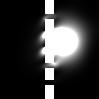
\includegraphics[width=.19\linewidth]{jko/congestion/holes-kappa10-5}&
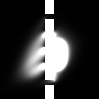
\includegraphics[width=.19\linewidth]{jko/congestion/holes-kappa10-10}&
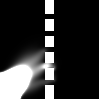
\includegraphics[width=.19\linewidth]{jko/congestion/holes-kappa10-20}\\
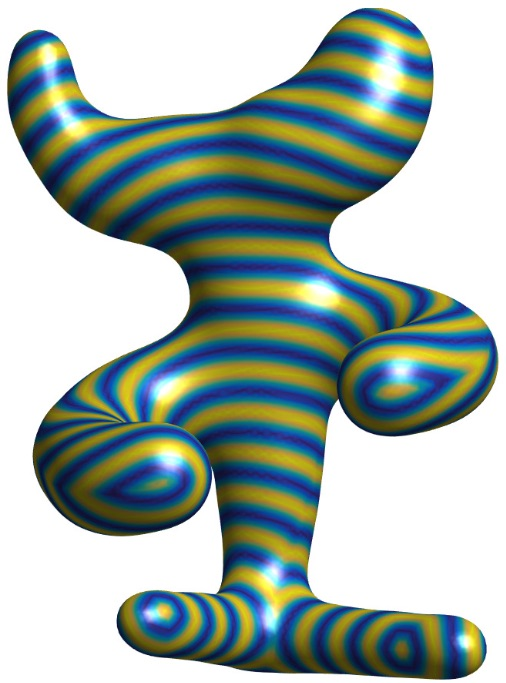
\includegraphics[width=.19\linewidth]{jko/surfaces/cosw}&
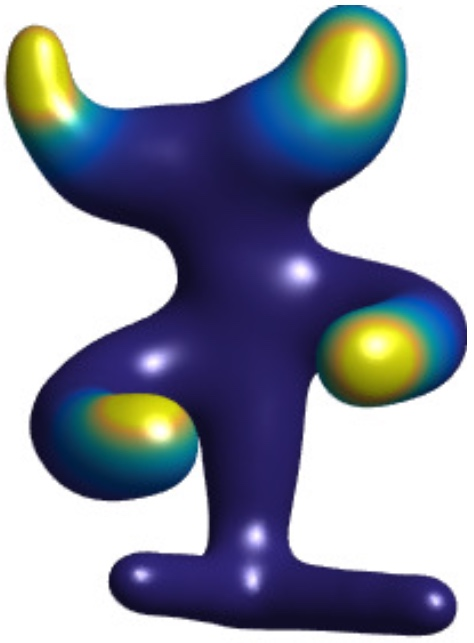
\includegraphics[width=.19\linewidth]{jko/surfaces/evol-1}&
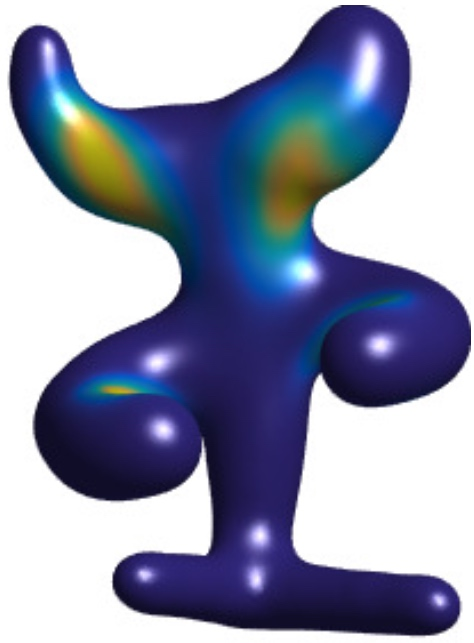
\includegraphics[width=.19\linewidth]{jko/surfaces/evol-2}&
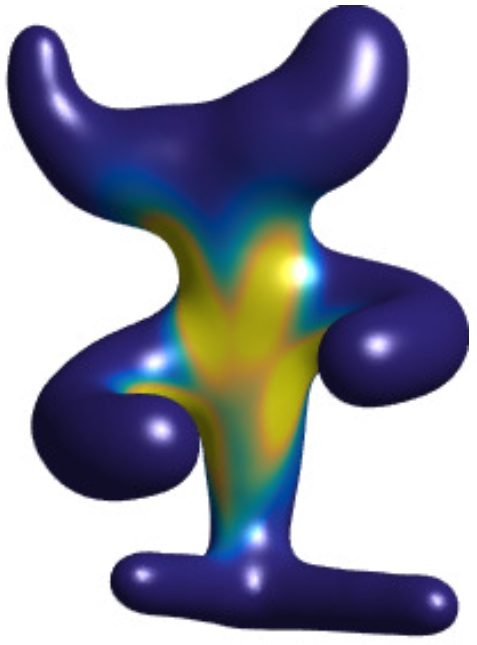
\includegraphics[width=.19\linewidth]{jko/surfaces/evol-3}&
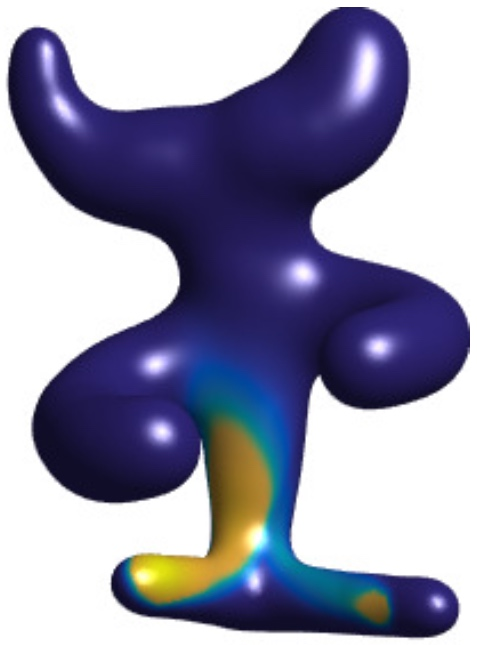
\includegraphics[width=.19\linewidth]{jko/surfaces/evol-4}\\
$\cos(w)$ & $t=0$ & $t=5$ & $t=10$ & $t=20$
\end{tabular}
\caption{\label{fig-jko}
ドリフト$V$と混雑項を伴う勾配流発展の例（~\citet{2015-Peyre-siims}より）。$F(\al) = \int_\X V(x) \d \al(x) + \iota_{\leq \kappa}(\density{\al})$である。
}
\end{figure}



\S\ref{sec-unbalanced}で詳述される非均衡最適輸送距離に対しても勾配流を計算することが可能である。これにより質量の生成または消滅を許容する発展が得られ、多くの物理的、生物学的、または化学的現象をモデル化する上で不可欠である。% Figure~\ref{fig-ot-grad-flows} shows
非均衡勾配流の例は、細胞成長のためのヘレ・ショー模型~\citep{PerthameTumor}であり、~\citep{gallouet2017jko,marino2017tumor}で理論的に研究されている。このような非均衡勾配流も一般化シンクホーンアルゴリズム~\citep{2016-chizat-sinkhorn}を用いて近似できる。


%\begin{figure}[h!]
%\centering
%
\includegraphics[width=.8\linewidth]{jko/heleshaw_profile}
%\caption{\label{fig-ot-grad-flows}
%Unbalanced OT gradient flow to solve the Hele-Shaw equation (from~\citep{2016-chizat-sinkhorn}). \todoK{detail the functional involved}
%}
%\end{figure}


%%%%%%%%%%%%%%%%%%%%%%%%%%%%%%%%%%%%%
%%%%%%%%%%%%%%%%%%%%%%%%%%%%%%%%%%%%%
%%%%%%%%%%%%%%%%%%%%%%%%%%%%%%%%%%%%%
%%%%%%%%%%%%%%%%%%%%%%%%%%%%%%%%%%%%%
\section{最小カントロヴィッチ推定量}
\label{sec-mke}

ある未知の分布からの離散サンプル$(x_i)_{i=1}^n \subset \Xx$が与えられたとき、目的はパラメトリックモデル$\th \mapsto \al_\th \in \Mm(\Xx)$を観測された経験入力測度$\be$にフィッティングすることである
\eql{\label{eq-density-fitting}
	\umin{\th \in \Theta} \Ll(\al_\th,\be)
	\qwhereq
	\be = \frac{1}{n} \sum_i \de_{x_i},
}
ここで$\Ll$は離散分布と「連続」（任意の）分布の間のある「損失」関数である（図~\ref{fig-density-fitting}参照）。

$\al_\th$がルベーグ測度（または他の固定された参照測度）に関する密度$\density{\th} \eqdef \density{\al_\th}$を持つ場合、最尤推定量（MLE）は以下を解くことで得られる
\eq{
	\umin{\th} \Ll_{\text{MLE}}(\al_\th,\be) \eqdef -\sum_i \log(\density{\th}(x_i)).
}
これは、$x_i$がある$\bar\be$のi.i.d.サンプルであると仮定すると、カルバック・ライブラー損失の経験的対応物を使用することに対応する。なぜなら
\eq{
	\Ll_{\text{MLE}}(\al,\be) \overset{n \rightarrow +\infty}{\longrightarrow} \KL(\al|\bar\be).
}
であるからである。

\begin{figure}[h!]
\centering

\includegraphics[width=.4\linewidth]{density-fitting/schematic-fitting}
\caption{\label{fig-density-fitting}
密度フィッティング問題~\ref{eq-density-fitting}の模式図。
}
\end{figure}


\newcommand{\fPF}{h}

このMLEアプローチは多くの場合に最適な推定手続きをもたらすことが知られている（例えば~\citet{owen2001empirical}参照）。しかし、特異な分布を推定する場合、典型的には$\al_\th$が密度を持たない場合（$\Ll_{\text{MLE}}(\al_\th,\be) = +\infty$となる）、または$(x_i)_i$がある特異な$\bar\be$からのサンプルである場合（$\KL(\al_\th|\bar\be)$が有限であるためには$\al_\th$が$\be$と同じ台を共有すべきであるが、この台は通常未知である）にはうまく機能しない。もう一つの問題は、実用上の関心が高い場合のいくつかにおいて、密度$\density{\th}$が計算できない（または計算が困難すぎる）ことである。

両方の問題（特異性と未知の密度）が生じる典型的な設定は、いわゆる生成モデルであり、パラメトリック測度は固定された参照測度$\zeta \in \Mm(\Zz)$の押し出しとして書かれる
\eq{
	\al_\th = \fPF_{\th,\sharp} \zeta \qwhereq \fPF_\th : \Zz \rightarrow \Xx,
}
ここで押し出し作用素は定義~\ref{defn-pushfwd}で導入されている。空間$\Zz$は通常低次元であるため、$\al_\th$の台は低次元の「多様体」に沿って局在化し、結果として得られる密度は高度に特異的である（ルベーグ測度に関する密度を持たない）。
%
さらに、この密度の計算は通常計算困難であるが、$\al_\th$からのi.i.d.サンプルの生成は$x_i=\fPF_\th(z_i)$を計算することで達成される。ここで$(z_i)_i$は$\zeta$からのi.i.d.サンプルである。

このような困難なシナリオに対処するためには、MLE汎関数$\Ll_{\text{MLE}}$の代わりに弱い距離を使用する必要があり、それは双対形式として
\eql{\label{eq-dual-loss}
	\Ll(\al,\be) \eqdef
	\umax{(\f,\g) \in \Cc(\X)^2}
	\enscond{ \int_{\X} \f(x) \d\al(x) + \int_{\X} \g(x) \d\be(x) }{ (\f,\g) \in \Potentials}.
}
と書く必要がある。\S\ref{sec-dual-norms}で示される双対ノルムは
\eq{
	\Potentials = \enscond{(\f,-\f)}{\f \in B},
}
を課すことに対応し、最適輸送~\eqref{eq-dual-generic}は$\Potentials = \Potentials(\c)$を~\eqref{eq-dfn-pot-dual}で定義されたように設定する。

固定された$\th$に対して、このような損失関数を用いて~\eqref{eq-density-fitting}で最小化すべきエネルギーを評価することは、半離散最適輸送を解くことに対応し、これは第~\ref{c-algo-semidiscr}章の焦点である。$\th$に関してエネルギーを最小化することははるかに複雑であり、典型的には高度に非凸である。

$\Ee(\th) = \Ll(\al_\th,\be)$を評価する際の~\eqref{eq-dual-loss}の解を$\f_\th$と表記すると、劣勾配は公式
\eql{\label{eq-grad-wass-loss-dual}
	\nabla \Ee(\th) = \int_\Xx [\partial \fPF_\th(x)]^\top \nabla \f_\th(x) \d\al_\th(x),
}
を用いて得られる。ここで$\partial \fPF_\th(x) \in \RR^{\text{dim}(\Theta) \times \dim}$は$\th \in \RR^{\text{dim}(\Theta)} \mapsto \fPF_\th(x)$の（$\th$に関する）微分であり、$\nabla \f_\th(x)$は$\f_\th$の（$x$に関する）勾配である。
%
この公式は数値的に使用するのが困難である。まず、半離散問題の解である連続関数$\f_\th$を計算する必要があるからである。\S\ref{sec-entropy-ot-mmd}で示されるように、最適輸送損失に対しては確率的最適化を用いて達成できるが、高次元では困難である。もう一つの選択肢は、このポテンシャルに対してパラメトリックな形式、例えばRKHSにおける展開（\citet{genevay2016stochastic}）や深層ネットワーク近似（\citep{WassersteinGAN}）を課すことである。しかし、これは理論的にはまだ解析されていない重要な近似誤差をもたらす。
%
最後の問題は、双対ポテンシャル$\f_\th$の勾配$\nabla \f_\th$の計算を必要とするため、数値的に不安定であることである。

最適輸送損失に対しては、以下の等価な問題に対する主最適結合を計算する方が、代替的な勾配公式が得られる：
\eql{\label{eq-ot-couplings-fitting}
	\MK_\c(\al_\th,\be) = \umin{\ga \in \Mm(\Zz \times \Xx)}
		\enscond{
			\int_{\Zz \times \Xx} c(\fPF_\th(z),x) \d\ga(z,x)
		}{
			\gamma \in \Couplings(\zeta,\be)
		}.
}
ここで考えている半離散の場合、最小化すべき目的関数は実際には以下のように分解できることに注意する
\eql{\label{eq-ot-couplings-fitting-bis}
	\umin{(\ga_i)_{i=1}^n} \sum_{i=1}^n \int_\Zz c(\fPF_\th(z),x_i) \d \ga_i(z)
	\qwhereq
	\sum_{i=1}^n \ga_i = \zeta, \quad
	\int_\Zz \d\ga_i(z)  = \frac{1}{n},
}
ここで各$\ga_i \in \Mm_+^1(\Zz)$である。
%
~\eqref{eq-ot-couplings-fitting-bis}を解く最適な$(\gamma_{\th,i})_i$が得られれば、$\Ee(\th)$の勾配は以下のように計算される
\eq{
	\nabla \Ee(\th) = \sum_{i=1}^n \int_\Zz [\partial \fPF_\th(z)]^\top \nabla_1 c(\fPF_\th(z),x_i) \d \ga_i(z),
}
ここで$\nabla_1 c(x,y) \in \RR^\dim$は$x \mapsto c(x,y)$の勾配である。~\eqref{eq-grad-wass-loss-dual}とは対照的に、この公式は双対最適輸送問題の解であるポテンシャルの勾配の計算を含まないことに注意する。

$\Ll=\MK_\c$を用いて得られるこの推定量のクラスは、しばしば「最小カントロヴィッチ推定量」と呼ばれ、~\citep{bassetti2006minimum}で最初に導入された。~\citep{CanasRosasco}も参照されたい。これは制限ボルツマンマシンの訓練のために~\citep{CuturiBoltzman}で生成モデルの文脈で使用され、近似ベイズ計算と組み合わせて~\citep{bernton2017inference}で使用されている。深層ネットワークを用いたこれらの計算の近似は、GAN~\citep{WassersteinGAN}とVAE~\citep{Bousquet2017}の両方の深層生成モデルの訓練に使用されている。~\citep{2017-Genevay-AutoDiff,2017-Genevay-gan-vae,salimans2018improving}も参照されたい。パラメトリックモデルフィッティングに対するシンクホーンダイバージェンスの使用は、形状マッチングおよびレジストレーションに日常的に使用されている。~\citep{gold1998new,chui2000new,myronenko2010point,2017-feydy-miccai}を参照されたい。


\begin{rem1}{距離学習と転移学習}
	機械学習への応用において、最適輸送関連手法の成功はデータの幾何学を捉えた適切なコスト$c(x,y)$の選択に大きく依存することを強調しておく。
	%
	多くの種類のデータをユークリッド空間に埋め込むことが可能であるが（例えば単語埋め込みについては~\citep{mikolov2013efficient}参照）、多くの場合、距離の何らかの適応または最適化が必要である。
	%
	教師あり課題に対する距離学習は古典的な問題であり（例えば~\citep{MAL-019,weinberger2009distance}参照）、学習パイプラインで最適輸送距離が使用される場合のグラウンド距離$c(x,y)$の学習に拡張されている~\citep{CuturiGroundMetric2014}（~\citealt{ZenICPR14,WangECCV12OLD,huang2016supervised}も参照されたい）。
	%
	また、最適結合$\P$の観測からコスト行列を学習するという関連する逆問題も挙げておく。これは低ランク事前分布を用いて正則化できる~\citep{dupuy2016estimating}。
	%
	関連する問題には転移学習~\citep{pan2010survey}とドメイン適応~\citep{glorot2011domain}があり、ここでは訓練済みの機械学習パイプラインを新しいデータセットに適応させたい。この問題は最適輸送技術を用いてモデル化および解くことができる。~\citep{courty2017optimal,courty2017joint}を参照されたい。
\end{rem1}

% !TEX root = ../ComputationalOTFnT.tex

\chapter{最適輸送の拡張}
\label{c-extensions}

この章では、最適輸送のKantorovich定式化に関連する（そして同じ構造を共有する）いくつかの変分問題を詳述する。目標は、最適輸送をより一般的な設定に拡張することである：複数の入力ヒストグラムおよび測度、正規化されていないもの、より一般的な測度のクラス、そして総輸送コストではなく局所的な正則性（ソース測度の近くの点がターゲット測度の近くの点に写像されるべき）に着目した測度間の最適輸送を含み、これら二つの測度が異なる距離空間に存在する場合も扱う。

%%%%%%%%%%%%%%%%%%%%%%%%%%%%%%%%%%%%%%%%%%%%%%%%%%%%%%%%%%%%%%%%%%%%%%%%%%
%%%%%%%%%%%%%%%%%%%%%%%%%%%%%%%%%%%%%%%%%%%%%%%%%%%%%%%%%%%%%%%%%%%%%%%%%%
%%%%%%%%%%%%%%%%%%%%%%%%%%%%%%%%%%%%%%%%%%%%%%%%%%%%%%%%%%%%%%%%%%%%%%%%%%
\section{多重周辺問題}
\label{sec-multimarginal}

Kantorovich定式化~\eqref{eq-mk-discr}を用いて二つの入力ヒストグラムを結合する代わりに、$S$個のヒストグラム$(\a_s)_{s=1}^S$（ただし$\a_s \in \simplex_{n_s}$）を以下の多重周辺問題を解くことにより結合することができる：
\eql{\label{eq-multimarginal-discr}
	\umin{\P \in \CouplingsD(\a_s)_s}
		\dotp{\C}{\P} \eqdef \sum_s \sum_{i_s=1}^{n_s} \C_{i_1,\ldots,i_S} \P_{i_1,\ldots,i_S},
}
ここで有効なカップリングの集合は
\eq{
	\CouplingsD(\a_s)_s = \enscond{\P \in \RR^{n_1 \times \ldots \times n_S}}{
		\foralls s, \foralls i_s, \sum_{\ell \neq s} \sum_{i_\ell=1}^{n_\ell}  \P_{i_1,\ldots,i_S} = \a_{s,i_s}
	}.
}
エントロピー正則化スキーム~\eqref{eq-regularized-discr}はこの設定に自然に拡張され
\eq{
	\umin{\P \in \CouplingsD(\a_s)_s}
		\dotp{\P}{\C} - \varepsilon \HD(\P),
}
Sinkhornアルゴリズムを適用して最適な$\P$をスケーリング形式で計算できる。ここで各エントリはマルチインデックスベクトル$i=(i_1,\ldots,i_S)$によりインデックスされる
\eq{
		\P_i = \K_i \prod_{s=1}^S \uD_{s,i_s}
		\qwhereq
		\K \eqdef e^{-\frac{\C}{\varepsilon}},
}
ここで$\uD_s \in \RR_+^{n_s}$は（未知の）スケーリングベクトルであり、$s=1,\ldots,S$を繰り返し巡回することにより反復的に更新される、
\eql{\label{eq-sinkh-multimarg}
	\uD_{s,i_s} \leftarrow
	\frac{ \a_{s,i_s} }{
		\sum_{\ell \neq s} \sum_{i_\ell=1}^{n_\ell}  \K_i \prod_{r \neq s} \uD_{\ell,i_r}
	}
}.

%%%%%%%%%%%%%%%%%%%%%
\begin{rem2}{一般の測度}
離散多重周辺問題~\eqref{eq-multimarginal-discr}は、空間$(\X_1,\ldots,\X_S)$上の測度$(\al_s)_s$に対してカップリング測度を計算することにより一般化される
\eql{\label{eq-multi-marginal-generic}
	\umin{\pi \in \Couplings(\al_s)_s} \int_{\X_1 \times \ldots \times \X_S} c(x_1,\ldots,x_S) \d\pi(x_1,\ldots,x_S),
}
ここでカップリングの集合は
\eq{
	\Couplings(\al_s)_s \eqdef \enscond{ \pi \in \Mm_+^1(\X_1 \times \ldots \times \X_S) }{
		\foralls s=1,\ldots,S, P_{s,\sharp} \pi = \al_s,
	}
}
ただし$P_s : \X_1 \times \ldots \times \X_S \rightarrow \X_s$は第$s$成分への射影であり、$P_s(x_1,\ldots,x_S)=x_s$である；例えば~\citep{GangboSciech}を参照。
%
多重周辺OT問題の主要な性質のレビューについては~\citep{PassMultiReview,PassMultiMarginalStructure}を参照されたい。
%
多重周辺OTの典型的な応用は、量子化学問題の解の近似計算であり、特に密度汎関数理論~\citep{CotarDFT,GorSeiVig,BuDePGor}における応用がある。この問題は特異なCoulomb相互作用コスト
\eq{
	c(x_1,\ldots,x_S) = \sum_{i \neq j} \frac{1}{\norm{x_i-x_j}}.
}
を考える場合に得られる。
\end{rem2}
%%%%%%%%%%%%%%%%%%%%%



%%%%%%%%%%%%%%%%%%%%%
\begin{rem2}{重心の多重周辺定式化}\label{eq-multimarg-bary}
	線形計画最適化~\eqref{eq-barycenter-generic}を、$\X^{S+1}$上の単一のカップリングに関する最適化として再定式化することが可能である。ここで最後の周辺分布が重心であり、他のものは入力測度$(\al_s)_{s=1}^S$である
	\eql{\label{eq-bary-multi-full}
		\umin{ \bar \pi \in \Mm_+^1(X^{S+1}) }
			\int_{\X^{S+1}} \sum_{s=1}^S \la_s c(x,x_s) \d\bar\pi(x_1,\ldots,x_s,x)
	}
	\eq{
		\text{subject to} \quad
				\foralls s=1,\ldots,S, \quad P_{s,\sharp}\bar\pi=\al_s.
	}
	これは「貼り合わせ補題」に由来する。この補題は、カップリング$(\pi_s)_{s=1}^S$（ただし$\pi_s \in \Couplings(\al_s,\al)$）が与えられたとき、周辺分布として$\pi_s$を持つ高次元カップリング$\bar \pi \in \Mm_+^1(X^{S+1})$を構成できる、すなわち$Q_{s\sharp}\bar\pi=\pi_s$（ただし$Q_s(x_1,\ldots,x_S,x) \eqdef (x_s,x) \in \X^2$）が成り立つことを述べている。
	\todoK{also relate this to celebrated result in graphical model, see book of Wainright/Jordan}
	%
	~\eqref{eq-bary-multi-full}において最後の周辺分布（$x \in \X$に対応する）に関して明示的に最小化することにより、重心問題~\eqref{eq-barycenter-generic}の解$\al$は$\al = A_{\la,\sharp} \pi$として計算できることが得られる。ここで$A_\la$は以下のように定義される「重心写像」である
	\eq{
		A_\la : (x_1,\ldots,x_S) \in \X^S \mapsto
		\uargmin{x \in \X} \sum_s \la_s c(x,x_s)
	}
	（この写像が一価であると仮定する）、ここで$\pi$はコスト
	\eql{\label{eq-cost-bary-multi}
		c(x_1,\ldots,x_S) = \sum_\ell \la_\ell c(x_\ell, A_\la(x_1,\ldots,x_S)).
	}
	を持つ多重周辺問題~\eqref{eq-multi-marginal-generic}の任意の解である。
	例えば、$c(x,y)=\norm{x-y}^2$の場合、定数の二乗項を除くと、
	\eq{
		c(x_1,\ldots,x_S) = -\sum_{r \leq s} \la_r \la_s \dotp{x_r}{x_s},
	}
	となり、これは~\citet{GangboSciech}で研究された問題である。
	%
	詳細については~\citet{Carlier_wasserstein_barycenter}を参照されたい。
	%
	この公式は、すべての入力測度が離散的$\be_s = \sum_{i_s=1}^{n_s} \a_{s,i_s} \de_{x_{s,i_s}}$である場合、
	重心$\al$もまた離散的であり、次の公式を用いて得られることを示す
	\eq{
		\al = \sum_{(i_1,\ldots,i_S)} \P_{(i_1,\ldots,i_S)}
			\de_{ A_\la(x_{i_1},\ldots,x_{i_S}) },
	}
	ここで$\P$はコスト行列$\C_{i_1,\ldots,i_S} = c(x_{i_1},\ldots,x_{i_S})$
	（~\eqref{eq-cost-bary-multi}で定義される）を持つ~\eqref{eq-multimarginal-discr}の最適解である。$\P$は$\sum_s n_s-S+1$個の等式制約を持つ線形計画問題の解として得られる$\prod_s n_s$次元の非負テンソルであるから、最大$\sum_s n_s-S+1$個の非零値を持つ最適解$\P$を得ることができる。したがって、最大$\sum_s n_s-S+1$個の点からなる台を持つ重心$\al$を得ることができる。この結果と離散の場合に関する他の考察は~\citet{anderes2016discrete}に見出すことができる。
\end{rem2}
%%%%%%%%%%%%%%%%%%%%%

%%%%%%%%%%%%
\begin{rem2}{Euler方程式の緩和}
非圧縮流体力学のEuler方程式の凸緩和が~\citeauthor{BrenierGeneralized}（\citeyear{BrenierEulerAMS}, \citeyear{BrenierEulerARMA}, \citeyear{BrenierEulerCPAM}, \citeyear{BrenierGeneralized}）および\citep{AmbrosioFigalliEuler}によって提案されている。
%
~\S\ref{sec-entropic-dynamic}で述べた設定と同様に、これはすべての経路$\ga : [0,1] \rightarrow \Xx$の集合$\bar\Xx$上の確率分布$\bar\pi \in \Mm_+^1(\bar\Xx)$を見出す問題に対応する。この確率分布は流体中の粒子の運動を記述する。
%
これは初期の偏微分方程式モデルの緩和版である。なぜなら、OTのKantorovich定式化と同様に、質量を分割できるからである。時間に伴う発展は、基礎空間$\X$の微分同相写像を必ずしも定義しない。
%
流体の力学は、~\eqref{eq-ot-pathsspace}と同様に各経路のエネルギー$\int_0^1 \norm{\ga'(t)}^2 \d t$を最小化することにより得られる。
%
経路空間上のOTとの違いは、流体の追加的な非圧縮性にある。
この非圧縮性は、粒子の密度が任意の時刻$t \in [0,1]$において一様であるべきことを課すことで処理される（古典的なOTのように初期時刻と最終時刻$t \in \{0,1\}$においてのみ課されるのではない）。$\X$がコンパクトであると仮定し、$\rho_{\Xx}$を$\Xx$上の一様分布とすると、これは$\bar P_{t,\sharp} \bar\pi = \rho_{\Xx}$と書ける。ここで$\bar P_t : \ga \in \bar\X \rightarrow \ga(t) \in \X$である。
%
この問題は、連続経路$(\ga(t))_{t \in [0,1]}$を格子$(x_k)_{k=1}^n \subset \X$上の$S$個の点の列$(x_{i_1}, x_{i_2},\ldots,x_{i_S})$で置き換えることにより離散化でき、$\bar\Pi$は$S$方向カップリング$\P \in \RR^{n^S} \in \Couplings(\a_s)_s$で表現される。ここで周辺分布は一様$\a_s=n^{-1} \ones_n$である。
%
対応する多重周辺問題のコストは
\eql{\label{eq-separable-euler}
	\C_{i_1,\ldots,i_S} = \sum_{s=1}^{S-1} \norm{x_{i_s}-x_{i_{s+1}}}^2 + R \norm{x_{\sigma(i_1)}-x_{i_{S}}}^2.
}
ここで$R$は十分大きなペナルティ定数であり、初期時刻と最終時刻の間の粒子の運動を強制するためのものである。この運動は置換$\sigma : \range{n} \rightarrow \range{n}$により規定される。
%
この結果として得られる多重周辺問題は、コストの特殊な構造を利用してSinkhorn反復~\eqref{eq-sinkh-multimarg}と組み合わせて効率的に実装される。これは~\citep{2015-benamou-cisc}で詳述されている。
%
実際、~\eqref{eq-sinkh-multimarg}に現れる分母の計算に必要な$O(n^S)$のコストの代わりに、$S$回の行列--ベクトル積の連鎖に分解でき、したがって低コスト$Sn^2$で計算できる。
%
他のソルバーも提案されており、例えば~\S\ref{s-semidiscrete}で示された半離散の枠組みを用いたものがある；~\citep{deGoes2015,gallouet2017lagrangian}を参照。
\end{rem2}
%%%%%%%%%%%%


%%%%%%%%%%%%%%%%%%%%%%%%%%%%%%%%%%%%%%%%%%%%%%%%%%%%%%%%%%%%%%%%%%%%%%%%%%
%%%%%%%%%%%%%%%%%%%%%%%%%%%%%%%%%%%%%%%%%%%%%%%%%%%%%%%%%%%%%%%%%%%%%%%%%%
%%%%%%%%%%%%%%%%%%%%%%%%%%%%%%%%%%%%%%%%%%%%%%%%%%%%%%%%%%%%%%%%%%%%%%%%%%
\section{非均衡最適輸送}
\label{sec-unbalanced}

通常の形の最適輸送の主要なボトルネックは、二つの入力測度$(\al,\be)$が同じ総質量を持つことを要求する点にある。多くの回避策が提案されているが（入力測度の正規化や、\S~\ref{sec-dual-norms}で詳述されたような双対ノルムの使用を含む）、満足のいく統一理論が開発されたのは最近のことである。ここでは単純だが重要な特殊ケースのみを概説する。

\citet{LieroMielkeSavareLong}に従い、任意の正のヒストグラム$(\a,\b) \in \RR_+^n \times \RR_+^m$を扱うために、元のKantorovich定式化~\eqref{eq-mk-discr}は、~\eqref{eq-discr-diverg}で定義されたダイバージェンス$\DivergmD_\phi$を用いて周辺分布の逸脱のみをペナルティすることにより「緩和」される。これは同等に、近似的な測度間のOT距離を最小化することに対応する
\begin{align}\label{eq-unbalanced-pbm}
	\MKD_{\C}^\tau(\a,\b) &= \umin{\tilde\a,\tilde\b} \MKD_{\C}(\a,\b) + \tau_1 \DivergmD_\phi(\a,\tilde \a) + \tau_2 \DivergmD_\phi(\b,\tilde\b) \\
		&= \umin{\P \in \RR_+^{n \times m}} \dotp{\C}{\P} + \tau_1\DivergmD_\phi(\P\ones_m|\a) + \tau_2\DivergmD_\phi(\P^\top\ones_m|\b),
\end{align}
ここで$(\tau_1,\tau_2)$は質量の輸送に対して質量変動をどの程度ペナルティするかを制御する。$\tau_1=\tau_2 \rightarrow +\infty$の極限において、$\sum_i \a_i=\sum_j \b_j$（「均衡」の場合）を仮定すると、ハードな周辺制約を持つ元の最適輸送定式化~\eqref{eq-mk-discr}が回復される。

この定式化は多くの先行研究を回復する。例えば$\DivergmD_\phi$として$\ell^2$ノルム~\citep{benamou2003numerical}や部分輸送~\citep{FigalliPartial,CaffarelliMcCannPartial}における$\ell^1$ノルムを導入する場合である。
%
特に重要なケースは、注意~\ref{rem-wfr-static}で詳述されるようにKullback--Leiblerダイバージェンスとして$\DivergmD_\phi=\KLD$を用いる場合である。
%
このコストに対して、$\tau=\tau_1=\tau_2 \rightarrow 0$の極限において、いわゆるHellinger距離の二乗（例~\ref{exmp-hellinger}も参照）が得られる
\eq{
	\MKD_{\C}^\tau(\a,\b) \overset{\tau \rightarrow 0}{\longrightarrow}
	\Hellinger^2(\a,\b) = \sum_i ( \sqrt{\a_i}-\sqrt{\b_i} )^2.
}

Sinkhorn反復~\eqref{eq-sinkhorn}は、~\S\ref{sec-generalized}で詳述された一般化アルゴリズムを利用することにより、この問題に適応できる。解は~\eqref{eq-scaling-form}の形を持ち、スケーリングは以下のように更新される
\eql{\label{eq-iterate-gen-sinkh}
	\uD \leftarrow \pa{ \frac{\a}{\K \vD} }^{\frac{\tau_1}{\tau_1+\varepsilon}}
	\qandq
	\vD \leftarrow \pa{ \frac{\b}{\transp{\K}\uD} }^{\frac{\tau_2}{\tau_2+\varepsilon}}.
}

%%%%%%%%%%%%%%%%%%%%%
\begin{rem2}{一般の測度}
$(\al,\be)$を二つの任意の測度とすると、~\eqref{eq-mk-generic}の非均衡版（「対数エントロピー」版とも呼ばれる）は次のようになる
\begin{align*}
	\MK_\c^\tau(\al,\be) \eqdef
	&\umin{\pi \in \Mm_+(\X \times \Y)}
		\int_{\X \times \Y} \c(x,y) \d\pi(x,y) \\
		&+ \tau \Divergm_\phi(P_{1,\sharp}\pi|\al)
		+ \tau \Divergm_\phi(P_{2,\sharp}\pi|\be),
\end{align*}
ここで測度間のダイバージェンス$\Divergm_\phi$は~\eqref{eq-phi-div}で定義される。
%
特殊ケース$c(x,y) = \norm{x-y}^2$、$\Divergm_\phi=\KL$において、$\MK_\c^\tau(\al,\be)^{1/2}$はGauss--Hellinger距離~\citep{LieroMielkeSavareLong}であり、$\Mm_+^1(\RR^d)$上の距離であることが示される。
\end{rem2}
%%%%%%%%%%%%%%%%%%%%%

%%%%%%%%%%%%%%%%%%%%%
\begin{rem2}{Wasserstein--Fisher--Rao}\label{rem-wfr-static}
特定のコストの選択
\eq{
	c(x,y) = -\log \cos(\min(\dist(x,y)/\kappa,\pi/2)),
}
ここで$\kappa$はあるカットオフ距離であり、$\Divergm_\phi=\KL$を用いると、
\eq{
	\WFR(\al,\be) \eqdef \MK_\c^\tau(\al,\be)^{\frac{1}{2}}
}
はいわゆるWasserstein--Fisher--Rao距離またはHellinger--Kantorovich距離である。
%
%
特殊ケース$\X=\RR^d$において、この静的な（Kantorovich型の）定式化は、~\citet{LieroMielkeSavareLong,2015-chizat-unbalanced}によって独立に証明されたように、その動的な対応物~\eqref{eq-wfr-dynamic}と一致する。この動的定式化は~\S\ref{dynamic-unbalanced}で詳述される。
%
%It is a distance on $\Mm_+^1(\X)$. In the special case $\X=\RR^d$, it also has a dynamic interpretation, which in some sense shows that it is the canonical extension of the $\Wass_2$ to the unbalanced case. It generalizes the initial Benamou-Brenier dynamical formulation~\eqref{eq-bb-convex} by introducing a source term $s_t(x)$ which is a scalar valued measure
%\begin{align*}
%	\WFR(\al_0,\al_1)^2 = &\umin{ (\al_t,\Moment_t,s_t)_t  \in \bar\BBConstr(\al_0,\al_1)  }
%		\int_0^1 \int_{\RR^d} \theta(\al_t(x),\Moment_t(x)) \\
%		& +  \theta(\al_t(x),s_t(x)) \d x \d t
%\end{align*}
%and the continuity equation reads
%\eq{
%	\bar\BBConstr(\al_0,\al_1) \eqdef
%	\enscond{ (\al_t,\Moment_t,s_t) }{
%		\pd{\al_t}{t} + \diverg(\Moment_t) = s_t,
%		\al_{t=0,1}=\al_{0,1}
%	}.
%}
%It can be solved using very similar methods to those detailed in Chapter~\ref{c-dynamic}.
\end{rem2}
%%%%%%%%%%%%%%%%%%%%%

重心問題~\eqref{eq-barycenter-generic}は、$\MK_{\c}$を$\MK_\c^\tau$で置き換えることにより非均衡の設定を扱えるように一般化できる。
%
図~\ref{fig-interpolation-static}は結果として得られる補間を示しており、緩和パラメータ$\tau$の有用性を良く示している。
%
入力測度は不等質量の二つのGauss分布の混合である。古典的なOTでは最も左のバンプを二つに分割する必要があり、非正則な補間を与える。対照的に、非均衡OTでは補間中に質量を変化させることができるため、バンプは分割されず、分布の局所的なモードが滑らかにマッチングされる。
%
有限の$\tau$値を用いること（OTは$\tau=\infty$に等しいことを思い出されたい）は、「ハードな」質量保存制約のために生じる質量分割による不規則な補間を防ぐために重要である。
%
結果として得られる最適化問題は、エントロピー正則化と~\S\ref{sec-generalized}で詳述された一般化Sinkhornアルゴリズムを用いて数値的に取り扱うことができる。

実際のところ、非均衡OT技法は、入力データがノイジーであるか完全には既知でない応用（画像処理や機械学習など）において古典的なOTを上回る性能を示すようである。また、総質量によって測定される測度の信号強度を考慮に入れるべき場合や、正規化が意味を持たない場合にも重要である。これは~\citet{FrognerNIPS}の元々の動機であり、彼らの目標は画像を記述するために用いられる単語ラベルの集合を比較することであった。非均衡OTと対応するSinkhorn反復は、~\citep{schiebinger2017reconstruction}における細胞のダイナミクスへの応用にも用いられている。

\begin{figure}[h!]
\centering
\begin{tabular}{@{}c@{\hspace{10mm}}c@{}}

\includegraphics[width=.4\linewidth]{unbalanced/ot-1} &

\includegraphics[width=.4\linewidth]{unbalanced/unbal-1} \\

\includegraphics[width=.4\linewidth]{unbalanced/ot-2} &

\includegraphics[width=.4\linewidth]{unbalanced/unbal-2} \\

\includegraphics[width=.4\linewidth]{unbalanced/ot-3} &

\includegraphics[width=.4\linewidth]{unbalanced/unbal-3} \\

\includegraphics[width=.4\linewidth]{unbalanced/ot-4} &

\includegraphics[width=.4\linewidth]{unbalanced/unbal-4} \\

\includegraphics[width=.4\linewidth]{unbalanced/ot-5} &

\includegraphics[width=.4\linewidth]{unbalanced/unbal-5} \\
Classical OT ($\tau=+\infty$) & Ubalanced OT ($\tau=1$)
\end{tabular}
%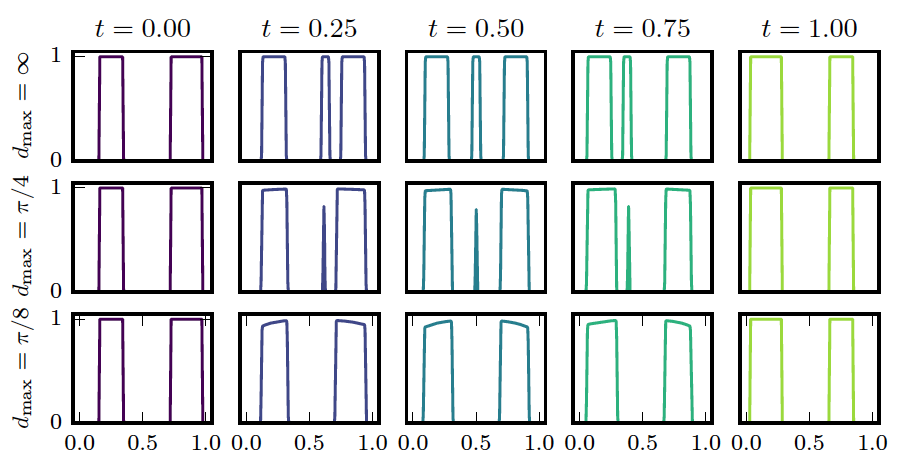
\includegraphics[width=\linewidth]{unbalanced/interpolation-static}
\caption{\label{fig-interpolation-static}
非均衡重心に対する緩和パラメータ$\tau$の影響。
上から下へ：二つの入力測度間における重心の推移。
}
\end{figure}


%%%
\begin{rem}[双対ノルムとの関連]\label{rem-unb-dualnorms}
質量変動を扱うための特に単純な設定は、~\S\ref{sec-dual-norms}で詳述されたように双対ノルムを用いることである。$\Cc(\X)$のコンパクト集合$B \subset \Cc(\X)$を選ぶことにより、$\Mm(\X)$全体の空間上で定義されるノルムが得られる（特に、測度は正である必要はない）。この設定の特殊なケースがフラットノルム~\eqref{eq-set-flatnorm}であり、これは全変動ノルム~\eqref{eq-defn-tv}として$\Divergm_\phi(\al|\al')=\norm{\al-\al'}_{\TV}$を用いた場合の非均衡輸送の特殊ケースとして回復される；例えば~\citep{hanin1992kantorovich,lellmann2014imaging}を参照。
%
Wasserstein-1非均衡輸送を定義するための一般的な枠組みについては~\citep{schmitzer2017framework}も参照されたい。
\end{rem}
%%%%

%%%%%%%%%%%%%%%%%%%%%%%%%%%%%%%%%%%%%%%%%%%%%%%%%%%%%%%%%%%%%%%%%%%%%%%%%%
%%%%%%%%%%%%%%%%%%%%%%%%%%%%%%%%%%%%%%%%%%%%%%%%%%%%%%%%%%%%%%%%%%%%%%%%%%
%%%%%%%%%%%%%%%%%%%%%%%%%%%%%%%%%%%%%%%%%%%%%%%%%%%%%%%%%%%%%%%%%%%%%%%%%%
\section{カップリングに対する追加制約を持つ問題}

他の多くのOT型の問題が文献で提案されている。これらは通常、元のOT問題~\eqref{eq-mk-generic}に現れる許容カップリングの集合に追加制約$\Cc$を加えることに対応する
\eql{\label{ot-extra-constr}
	\umin{\pi \in \Couplings(\al,\be)}
		\enscond{ \int_{\X \times \Y} \c(x,y) \d\pi(x,y) }{ \pi \in \Cc }.
}
二つの代表的な例を挙げる。
%
容量制約付き最適輸送~\citep{km1}は、密度$\density{\pi}$（例えばLebesgue測度に関する）が上に有界であることを課すものに対応する
\eql{\label{eq-capacity-constr}
	\Cc = \enscond{ \pi }{ \density{\pi} \leq \kappa }
}
ここで$\kappa>0$である。この制約はMonge写像上に局在化した特異カップリングを除外する。
%
マルチンゲール輸送問題（例えば~\citet{GalichonMartingale,dolinsky2014martingale,TanTouzi,beiglbock2013model}を参照）は、金融において多くの応用を見出すものであり、$\X=\Y=\RR^d$のとき、カップリングの条件付き平均にいわゆるマルチンゲール制約を課す：
\eql{\label{eq-martingale-constr}
	\Cc = \enscond{ \pi }{ \foralls x \in \RR^d,  \int_{\RR^d} y \frac{\d \pi(x,y)}{\d\al(x)\d\be(y)} \d\be(y) = x }.
}
この制約は、任意の許容カップリングの重心射影写像~\eqref{eq-bary-proj}が恒等写像に等しくなければならないことを課す。
%
任意の$(\al,\be)$に対して、この集合$\Cc$は通常空っぽであるが、$\Cc \neq \emptyset$を保証する（$\al$と$\be$が「凸順序」にあるべきという）必要十分条件が存在し、$(\al,\be)$がマルチンゲール制約を満たすようにする。この制約は既存の問題を離散化する際に数値的に課すことが困難な場合がある。
%
また、単一のMonge写像上に解が集中することを禁じ、複数のグラフの和集合上に集中するカップリング（「多価」Monge写像）、またはさらに複雑な台の集合につながりうる。
%
~\eqref{eq-entropic-generic}のようなエントロピーペナルティを用いることにより、~\citet{2015-benamou-cisc}で説明されたDykstraアルゴリズムを用いて~\eqref{ot-extra-constr}を近似的に解くことができる。これは~\S\ref{sec-sinkhorn}で示されたSinkhornアルゴリズムの一般化である。これには$\KL$ダイバージェンスに対する$\Cc$への射影の計算が必要であり、~\eqref{eq-capacity-constr}に対しては容易であるが~\eqref{eq-martingale-constr}に対しては閉じた形では計算できず、したがって副反復が必要となる；詳細は~\citep{guo2017computational}を参照。


%%%%%%%%%%%%%%%%%%%%%%%%%%%%%%%%%%%%%%%%%%%%%%%%%%%%%%%%%%%%%%%%%%%%%%%%%%
%%%%%%%%%%%%%%%%%%%%%%%%%%%%%%%%%%%%%%%%%%%%%%%%%%%%%%%%%%%%%%%%%%%%%%%%%%
%%%%%%%%%%%%%%%%%%%%%%%%%%%%%%%%%%%%%%%%%%%%%%%%%%%%%%%%%%%%%%%%%%%%%%%%%%
\section{スライスWasserstein距離と重心}\label{sec-sliced}

$\RR^\dim$上で定義された二つの測度$(\al,\be)$間の距離を、球面上のすべての方向への射影の1次元Wasserstein距離を集約することにより定義できる。これは以下を定義する
\eql{\label{eq-sw-def}
	\SW(\al,\be)^2 \eqdef \int_{\SS^d} \Wass_2( P_{\th,\sharp} \al, P_{\th,\sharp} \be )^2 \d\th,
}
ここで$\SS^\dim = \ensconds{\th \in \RR^\dim}{\norm{\th}=1}$は$\dim$次元球面であり、$P_\th : x \in \RR^\dim \rightarrow \RR$は射影である。このアプローチは~\citep{2013-Bonneel-barycenter}で詳述されており、Marc Bernotのアイデアに基づいている。これは測度空間上のRadon逆変換の問題~\citep{AbrahamRadon}に関連している。

%%%
\paragraph{Lagrange離散化と確率的勾配降下法}

この汎関数の利点は、1次元Wasserstein距離が~\S\ref{sec:specialcases}で詳述されているように容易に計算できることである。$m=n$かつ
\eql{\label{eq-lagrangian-sliced}
	\al=\frac{1}{n}\sum_{i=1}^n \de_{x_i}
	\qandq
	\be=\frac{1}{n}\sum_{i=1}^m \de_{y_i},
}
の特殊ケースでは、これは単に点をソートすることで達成される
\eq{
	\SW(\al,\be)^2 = \int_{\SS^d} \pa{
		 \sum_{i=1}^n | \dotp{ x_{\si_\th(i)} - y_{\kappa_\th(i)} }{\th} |^2
		}
		\d\th,
}
ここで$\si_\th,\kappa_\th \in \Perm(n)$はそれぞれ$(\dotp{x_i}{\th})_i$と$(\dotp{y_i}{\th})_i$を昇順に並べる置換である。

ベクトル$y$を固定すると、関数$\Ee_\be(x) \eqdef \SW(\al,\be)^2$は滑らかであり、この関数を用いて勾配降下法により写像を定義できる
\eql{\label{eq-grad-sliced-lagr}
	x \leftarrow x - \tau \nabla\Ee_\be(x)
	\qwhereq
}
\eq{
	\nabla\Ee_\be(x)_i =
		2 \int_{\SS^d} \pa{
		 	\dotp{ x_{i} - y_{\kappa_\th \circ \si_\th^{-1}(i)} }{\th}  \th
		}
		\d\th
}
ここで十分小さなステップサイズ$\tau>0$を用いる。
%
この方法を扱いやすくするために、確率的勾配降下法（SGD）を用いて、この積分をランダムに抽出された方向$\th \in \SS^\dim$に対する離散和で置き換えることができる（SGDの詳細については~\S\ref{sec-sgd}を参照）。
%
フロー~\eqref{eq-grad-sliced-lagr}は、関数$\al \mapsto \SW(\al,\be)^2$のWasserstein勾配流（~\S\ref{sec-grad-flows}の意味で）の（Lagrange的実装と）理解できる。数値的には、このフローは局所的最小値を持たず、したがって$\al=\be$に収束することが見出される。Lagrangeソルバーの有用性は、収束時に二つの分布間のマッチング（Monge写像に類似したもの）を定義することである。この方法は~\citep{rabin-ssvm-11}において色転写とテクスチャ合成に成功裏に用いられており、~\citep{pitie2007automated}で詳述された交互最小化アプローチに関連している。

このLagrangeスキームを拡張して、測度の近似的な「スライス」重心を計算することは容易であり、Wasserstein重心のFrechet定義~\eqref{eq-barycenter-generic}を模倣して以下を最小化する
\eql{\label{eq-barycenter-sliced}
		\umin{\al \in \Mm_+^1(\X)} \sum_{s=1}^S \la_s \SW(\al,\be_s)^2,
}
ここで$(\be_s)_{s=1}^S$は固定された入力測度の集合である。$\al$と$(\be_s)_s$の両方に対して~\eqref{eq-lagrangian-sliced}の形のLagrange離散化を用いて、位置$x=(x_i)_i$に関する非凸最小化を実行できる
\eql{\label{eq-bary-lagrangian-sliced}
	\umin{x} \Ee(x) \eqdef \sum_{s} \la_s \Ee_{\be_s}(x),
	\qandq
	\nabla \Ee(x) = \sum_{s} \la_s \nabla \Ee_{\be_s}(x),
}
ここで$\nabla \Ee_{\be_s}(x)$の計算には公式~\eqref{eq-grad-sliced-lagr}を用いた勾配降下法（方向$\th$のランダムサンプリングと組み合わせて）を使用する。




%%%
\paragraph{Euler離散化とRadon変換}

反復的な最小化スキームに頼ることなく近似的なスライス重心を計算する関連する方法は、~\eqref{eq-sw-def}がRadon変換$\Rr(\al)$と$\Rr(\be)$の間の距離を計算するという事実を利用することである。ここで
\eq{
	\Rr(\al) \eqdef ( P_{\th,\sharp} \al )_{\th \in \SS^d}.
}
重要な点は、Radon変換が可逆であり、その逆がフィルタ補正逆投影公式を用いて計算できることである。
%
測度の集合$\rho = (\rho_\th)_{\th \in \SS^d}$が与えられたとき、フィルタ補正逆投影作用素を以下のように定義する
\eql{\label{eq-filter-backproj}
	\Rr^+(\rho) = C_\dim \De^{\frac{d-1}{2}} \Bb(\rho),
}
ここで$\xi = \Bb(\rho) \in \Mm(\RR^d)$は以下の関係を通じて定義される測度である
\eql{\label{eq-backproj}
	\foralls g \in \Cc(\RR^d), \quad
	\int_{\RR^d} g(x) \d\xi(x) =
	\int_{\SS^d}  \int_{\RR^{\dim-1}}   \int_{\RR}
		g( r \th + U_\th z )
	\d \rho_\th(r) \d z \d \th,
}
ここで$U_\th$は$\th^\bot$の任意の正規直交基底であり、
$C_\dim \in \RR$は次元に依存する正規化定数である。
%
ここで$\De^{\frac{d-1}{2}}$は分数次Laplacianであり、Fourier領域上で
$\hat \De^{\frac{d-1}{2}}(\om) = \norm{\om}^{d-1}$として定義されるハイパスフィルタである。
%
逆投影~\eqref{eq-backproj}の定義は、各測度$(\rho_\th)_\th$を$\th$に直交する方向に定数として拡張することにより、すべての測度の寄与を足し合わせる。
%
すると左逆関係$\Rr^+ \circ \Rr = \Identity_{\Mm(\RR^\dim)}$が成り立ち、$\Rr^+$は有効な再構成公式となる。


\newcommand{\MyFigRadon}[1]{\includegraphics[width=.19\linewidth]{radon-bary/#1}}
\begin{figure}[h!]
\centering
\begin{tabular}{@{}c@{\hspace{1mm}}c@{\hspace{1mm}}c@{\hspace{1mm}}c@{\hspace{1mm}}c@{}}
\MyFigRadon{bary-1} &
\MyFigRadon{bary-3} &
\MyFigRadon{bary-5} &
\MyFigRadon{bary-7} &
\MyFigRadon{bary-9} \\
\MyFigRadon{radon-1} &
\MyFigRadon{radon-3} &
\MyFigRadon{radon-5} &
\MyFigRadon{radon-7} &
\MyFigRadon{radon-9} \\
$t=0$ & $t=1/4$ & $t=1/2$ & $t=3/4$ & $t=1$
\end{tabular}
\caption{\label{fig-radon-bary}
Radon変換を用いたスライス重心計算の例（~\eqref{eq-barycenter-radon-sliced}で定義される通り）。
%
上段：$S=2$の二つの入力と重み$(\la_1,\la_2)=(1-t,t)$に対する重心$\al_t$。
下段：それらのRadon変換$\Rr(\al_t)$（水平軸は方位角$\th$）。
}
\end{figure}

入力密度の重心を計算するために、公式~\eqref{eq-barycenter-generic}をRadon変換を用いた等価な式で置き換え、各$\th$に対して独立に1次元重心問題を考えることは理にかなっている
\eql{\label{eq-barycenter-radon-sliced}
		\rho_\th^\star \in \uargmin{ (\rho_\th \in \Mm_+^1(\RR)) } \sum_{s=1}^S \la_s \Wass_2( \rho_\th, P_{\th,\sharp} \be_s)^2.
}
各1次元重心問題は、注意~\ref{rem-bary-1d}で詳述された単調再配置を用いて容易に計算される。
%
~\eqref{eq-barycenter-generic}を解くスライス重心のRadon近似$\al_{R} \eqdef \Rr^+( \rho^\star )$は、逆Radon変換$\Rr^+$により得られる。一般に$\al_R$は~\eqref{eq-barycenter-generic}の解ではないことに注意されたい。なぜなら、Radon変換は全射ではないため、Radon変換$\Rr(\be_s)$の重心として得られる$\rho^\star$は$\Rr$の値域に必ずしも属さないからである。しかし数値的には、実際にはほぼそうであるようである~\citep{2013-Bonneel-barycenter}。
%
数値的には、このRadon変換の定式化は、固定格子上に離散化された入力測度と重心（例えば画像の一様格子）に対して非常に効果的であり、$\Rr$および$\Rr^+$はこの格子上で高速アルゴリズムを用いて近似的に計算される（例えば~\citep{FastSlantStack}を参照）。
%
図~\ref{fig-radon-bary}はこの重心計算を示し（Radon変換がどのように補間されるかを強調している）、図~\ref{fig-sliced-bary-compar}はRadon重心~\eqref{eq-barycenter-radon-sliced}とLagrange離散化~\eqref{eq-bary-lagrangian-sliced}により得られた重心の比較を示す。


\begin{figure}[h!]
\centering
\begin{tabular}{@{}c@{\hspace{1mm}}c@{\hspace{1mm}}c@{}}

\includegraphics[width=.32\linewidth]{sliced/triangle-radon}&

\includegraphics[width=.32\linewidth]{sliced/triangle-sliced}&

\includegraphics[width=.32\linewidth]{sliced/triangle-wass} \\
Radon & Lagrangian & Wasserstein
\end{tabular}
\caption{\label{fig-sliced-bary-compar}
Radon変換~\eqref{eq-barycenter-radon-sliced}（Euler離散化）、Lagrange離散化~\eqref{eq-bary-lagrangian-sliced}、およびWasserstein OT（Sinkhorn反復~\eqref{eq-sinkhorn-bary}を用いて計算）による重心の比較。
}
\end{figure}



%%%
\paragraph{スライスWassersteinカーネル}

計算の単純さに加えて、スライスWasserstein距離のもう一つの利点は、注意~\ref{rem-1d-ot-generic}、特に公式~\eqref{eq-wass-cumul}で詳述されているように、Euclid距離と等距であること（すなわち「Hilbert的」計量であること）である。
%
~\S\ref{sec-non-embeddability}で強調されたように、これは$\RR^\dim$上のWasserstein距離$\Wass_2$と対照的であり、$\Wass_2$は次元$\dim \geq 2$においてHilbert的ではない。
%
したがって、このスライス距離を用いて、分布の空間$\Mm_1^+(\RR^\dim)$に再生核Hilbert空間構造を与えることが可能である（~\S\ref{sec-non-embeddability}で詳述されている通り）。
%
例えば、指数カーネルとエネルギー距離カーネル
\eq{
	\Krkhs(\al,\be) = e^{-\frac{\SW(\al,\be)^p}{2\si^p}}
	\qandq
	\Krkhs(\al,\be) = -\SW(\al,\be)^p
}
を使うことができる。ここで指数カーネルに対しては$1 \leq p \leq 2$、エネルギー距離カーネルに対しては$0 < p < 2$である。
%
これは、入力測度の任意の集合$(\al_i)_i$に対して、行列$( \Krkhs(\al_i,\al_j) )_{i,j}$が対称半正定値であることを意味する。これらのカーネルを用いて、「カーネルトリック」により、回帰、分類（SVMおよびロジスティック）、クラスタリング（K-means）、次元削減（PCA）~\citep{Hofmann2008}など、様々な機械学習タスクを実行することが可能である。
%
詳細と応用については~\citet{kolouri2016sliced}を参照されたい。



%%%%%%%%%%%%%%%%%%%%%%%%%%%%%%%%%%%%%%%%%%%%%%%%%%%%%%%%%%%%%%%%%%%%%%%%%%
%%%%%%%%%%%%%%%%%%%%%%%%%%%%%%%%%%%%%%%%%%%%%%%%%%%%%%%%%%%%%%%%%%%%%%%%%%
%%%%%%%%%%%%%%%%%%%%%%%%%%%%%%%%%%%%%%%%%%%%%%%%%%%%%%%%%%%%%%%%%%%%%%%%%%
\section{ベクトルと行列の輸送}

実数値測度$\al \in \Mm(\Xx)$は、ベクトル値測度$\al \in \Mm(\Xx;\VV)$に容易に一般化される。ここで$\VV$はあるベクトル空間である。記法の簡潔さのため、$\VV$はEuclid空間であり、ある内積$\dotp{\cdot}{\cdot}$を備えていると仮定する（典型的には$\VV=\RR^\dim$であり、内積は標準的なものである）。この内積のおかげで、ベクトル値測度は連続関数$g : \Xx \rightarrow \VV$の双対と同一視される。すなわち、任意のそのような$g$に対して、測度との積分は
\eql{\label{eq-integration-vec-valued}
	\int_\Xx g(x) \d\al(x) \in \RR,
}
と定義され、これは$g$と$\al$に関する線形作用素である。離散測度は$\al = \sum_i \a_i \de_{x_i}$の形を持ち、ここで$(x_i,a_i) \in \Xx \times \VV$であり、積分公式~\eqref{eq-integration-vec-valued}は単に
\eq{
	\int_\Xx g(x) \d\al(x) = \sum_i \dotp{\a_i}{g(x_i)} \in \RR.
}
と読める。
同値的に、$\VV=\RR^\dim$ならば、そのような$\al$は$\dim$個の「古典的な」実数値測度$(\al_s)_{s=1}^\dim$の集まり（その座標）と見なすことができ、
\eq{
	\int_\Xx g(x) \d\al(x) =  \sum_{s=1}^\dim \int_\Xx g_s(x) \d\al_s(x),
}
と書ける。ここで$g(x)=(g_s(x))_{s=1}^\dim$は$g$の標準基底における座標である。

%%%
\paragraph{双対ノルム}

OT距離をこのような一般的な設定に拡張することは自明ではなく、実際一般には不可能である。正と負の両方の値を取る実数値測度を扱うことさえ困難である。唯一の単純な選択肢は、~\S\ref{sec-dual-norms}で定義された双対ノルムを考えることである。実際、公式~\eqref{eq-w1-cont}は、$B$を$\Cc(\Xx;\VV)$の部分集合として考えることにより、$\Mm(\Xx;\VV)$に容易に拡張される。したがって特に、$\Ww_1$、フラットノルム、およびMMDノルムはベクトル値測度に対して計算できる。

%%%
\paragraph{錐値測度上のOT}

$\al$が部分集合$\Mm(\Xx;\Vv) \subset \Mm(\Xx;\VV)$に制限される場合、より高度なOT距離を定義することが可能である。集合$\Vv$は$\VV$の正の1次同次凸錐でなければならない
\eq{
	\Vv \eqdef \enscond{ \la u }{ \la \in \RR^+,  u \in \Vv_0, }
}
ここで$\Vv_0$はコンパクト凸集合である。
%
典型的な例は$\Vv=\RR_+^\dim$の正の測度の集合である。このような錐上のOTの動的凸定式化が提案されている；~\citep{MatthesPositive}を参照。これは化学成分の分布のモデリングに応用されている。
%
もう一つの重要な例は正対称行列$\Vv=\Ss_+^\dim \subset \RR^{\dim \times \dim}$の集合である。もちろん、行列をベクトルとして扱うことにより、この空間上の双対ノルムを使用することが可能である；例えば~\citep{Ning2014metrics}を参照。このような錐上のOTの動的凸定式化が提供されている~\citep{Chen2016,JiangSpectral}。いくつかの静的な（Kantorovich型の）定式化も提案されている~\citep{ning2015matrix,2016-peyre-qot}が、数学的に健全な理論的枠組みはまだ欠けている。特に、これらの静的アプローチがベクトル値測度に対する距離を定義するのか、また何らかの動的定式化に関連するのかは不明である。図~\ref{fig-tensors}は、~\citep{2016-peyre-qot}で詳述された方法を用いて得られたテンソル補間の例であり、この方法はテンソル場を扱うために量子相対エントロピー~\eqref{eq-quantum-entropy}を用いたSinkhornアルゴリズムの一般化を提案している。

%%%
\paragraph{正行列上のOT}

関連するが全く異なる設定は、離散測度、すなわちヒストグラム$\a \in \Si_n$を、単位トレースの正行列$A \in \Ss_n^+$（ただし$\tr(A)=1$）で置き換えることである。$A$の固有値$\la(A) \in \Si_n$がヒストグラムの役割を果たすという理由であるが、固有ベクトルの回転も考慮に入れる必要があるため、この問題はより複雑である。

~\S\ref{sec-phi-div}で導入されたいくつかのダイバージェンスをこの設定に拡張することができる。例えば、Bures計量~\eqref{eq-bure-defn}はHellinger距離（注意~\ref{exmp-hellinger}で定義）の一般化であり、正の対角行列上では一致する。
%
Kullback--Leiblerダイバージェンス~\eqref{eq-kl-defn}（注意~\ref{ex_KLdiv}も参照）も拡張でき、正行列に対して以下のように一般化される
\eql{\label{eq-quantum-entropy}
	\KLD(A|B) \eqdef \tr\pa{ P \log(P)-P\log(Q)-P+Q, }
}
ここで$\log(\cdot)$は行列対数である。この行列$\KLD$は両方の引数に関して凸である。

このような行列間のOT距離を定義するために、凸動的定式化を解くことが可能である~\citep{Carlen2014,Chen2016,ChenGangbo17}。Sinkhornアルゴリズムの等価物も存在し、~\citet{gurvits2004classical}に由来し、~\citep{georgiou2015positive}で広く研究されている；レビュー論文~\citep{ReviewSinkhorn}も参照。これはいくつかのケースでのみ収束することが知られているが、経験的には常に機能するようである。


\newcommand{\MyFigTensorMesh}[1]{\includegraphics[width=.100\linewidth,trim=140 10 120 0,clip]{tensors/mesh/interpol-#1}}
\newcommand{\MyFigTensorImg}[1]{\includegraphics[width=.105\linewidth,trim=80 20 80 20,clip]{tensors/2d/interpol-ellipses-#1}}
%%% FIG %%%
\begin{figure}[h!]\centering
\centering
\begin{tabular}{@{\hspace{1mm}}c@{\hspace{1mm}}c@{\hspace{1mm}}c@{\hspace{1mm}}c@{\hspace{1mm}}c@{\hspace{1mm}}c@{\hspace{1mm}}c@{\hspace{1mm}}c@{\hspace{1mm}}c@{}}
\MyFigTensorImg{1}&
\MyFigTensorImg{2}&
\MyFigTensorImg{3}&
\MyFigTensorImg{4}&
\MyFigTensorImg{5}&
\MyFigTensorImg{6}&
\MyFigTensorImg{7}&
\MyFigTensorImg{8}&
\MyFigTensorImg{9}\\
\MyFigTensorMesh{1}&
\MyFigTensorMesh{2}&
\MyFigTensorMesh{3}&
\MyFigTensorMesh{4}&
\MyFigTensorMesh{5}&
\MyFigTensorMesh{6}&
\MyFigTensorMesh{7}&
\MyFigTensorMesh{8}&
\MyFigTensorMesh{9}\\
$t=0$ & $t=1/8$ & $t=1/4$ & $t=3/8$ & $t=1/2$ & $t=5/8$ & $t=3/4$ & $t=7/8$ & $t=1$
\end{tabular}
%%%
\caption{%%%
ある領域（ここでは2次元平面正方形と曲面メッシュ）上の二つの入力半正定値行列場（時刻$t \in \{0,1\}$において楕円を用いて表示）間の補間。~\citet{2016-peyre-qot}で詳述された方法を使用。
%
線形補間スキームとは異なり、このOT的手法はテンソルの「質量」（楕円の大きさ）だけでなく、それらの異方性と方向も輸送する。
} \label{fig-tensors}
\end{figure}
%%% FIG %%%



%%%%%%%%%%%%%%%%%%%%%%%%%%%%%%%%%%%%%%%%%%%%%%%%%%%%%%%%%%%%%%%%%%%%%%%%%%
%%%%%%%%%%%%%%%%%%%%%%%%%%%%%%%%%%%%%%%%%%%%%%%%%%%%%%%%%%%%%%%%%%%%%%%%%%
%%%%%%%%%%%%%%%%%%%%%%%%%%%%%%%%%%%%%%%%%%%%%%%%%%%%%%%%%%%%%%%%%%%%%%%%%%
\section{Gromov--Wasserstein距離}

形状マッチングなどの一部の応用において、最適輸送距離の重要な弱点は、リスケーリング、平行移動、回転などの重要な不変性の族に対して不変ではないという事実にある。そのようなグローバル変換を扱うためのOTの非凸変形がいくつか提案されており~\citep{cohen1999earth,pele2013tangent}、最近では言語間単語埋め込みの整合~\citep{grave2018unsupervised,alvarez2018towards,grave2018unsupervised}などの問題に適用されているが、これらの方法はまず不変性の部分集合を指定する必要があり、可能性として異なる距離空間間で関連性を持たせる必要がある。この節では、不変性の族の定義を必要とせずに、異なる空間上で定義された測度を扱うことができる、より一般的で非常に自然なOTの拡張を記述する。

%%%%%%%%%%%%%%%%%%%%%%%%%%%%%%%%%%%%%%%%%%%%%%%%%%%%%%%%%%%%%%%%%%%%%%%%%%
\subsection{Hausdorff距離}
\label{sec-hausdorff}

ある距離$\dist_\Z$に対する二つの集合$A,B \subset \Z$間のHausdorff距離は
\eq{
	\Hh_\Zz(A,B) \eqdef \max\Big(
  		\sup_{a \in A} \inf_{b \in B} d_{\Zz}(a,b),
  		\sup_{b \in B} \inf_{a \in A} d_{\Zz}(a,b)
	\Big),
}
であり、図~\ref{fig-hausdorff}を参照。
%
これは$\Z$のコンパクト集合$\Kk(\Z)$間の距離を定義し、$\Z$がコンパクトならば$(\Kk(\Z),\Hh_\Zz)$自身もコンパクトである；~\citep{burago2001course}を参照。

\begin{figure}[h!]
\centering

\includegraphics[width=.26\linewidth]{gromov-hausdorff/hausdorff-1}
\qquad

\includegraphics[width=.26\linewidth]{gromov-hausdorff/hausdorff-2}
\caption{\label{fig-hausdorff}
$\RR^2$におけるHausdorff距離の計算。
}
\end{figure}

\citet{memoli-2011}に従って、集合$(A,B)$間のこの距離は、測度間のWasserstein距離と同様に定義できることに注意する（測度はある意味で「重み付き」集合と理解されるべきものである）。測度のカップリング~\eqref{eq-coupling-generic}を集合のカップリング
\eq{
	\Rr(A,B) \eqdef \enscond{ R \in \X \times \Y }{
	\begin{array}{l}
		\foralls a \in A, \exists b \in B, (a,b) \in R \\
		\foralls b \in B, \exists a \in A, (a,b) \in R
	\end{array}
	}.
}
で置き換える。
Kantorovich問題~\eqref{eq-mk-generic}に対して、積分（測度にアクセスできないため）を最大化で置き換えると、次式が得られる
\eql{\label{eq-hausf-couplings}
	\Hh_\Zz(A,B) = \uinf{ R \in \Rr(A,B) } \sup_{(a,b) \in R} d(a,b).
}
%
測度カップリング$\pi \in \Couplings(\al,\be)$の台は台の間の集合カップリングであること、すなわち$\Supp(\pi) \in \Rr( \Supp(\al),\Supp(\be) )$であることに注意されたい。
%
Hausdorff距離はしたがって$\infty$-Wasserstein距離（注意~\ref{rem-p-inf}を参照）に関連しており、台が$(A,B)$である任意の測度$(\al,\be)$に対して$\Hh(A,B) \leq \Wass_\infty(\al,\be)$が成り立つ。


%%%%%%%%%%%%%%%%%%%%%%%%%%%%%%%%%%%%%%%%%%%%%%%%%%%%%%%%%%%%%%%%%%%%%%%%%%
\subsection{Gromov--Hausdorff距離}

Gromov--Hausdorff（GH）距離~\citep{gromov-2001}（~\citep{edwards1975structure}も参照）は、二つの距離空間$(\X,d_\X), (\Y,d_\Y)$がどの程度互いに等距であることから離れているかを定量化することにより、それらの間の距離を測る方法であり、図~\ref{fig-gh}を参照。これは、二つの空間のすべての可能な等距的埋め込みについての最小Hausdorff距離として定義される
\eq{
	\Gg\Hh(d_\Xx,d_\Yy) \eqdef
	\inf_{\Zz,f,g} \enscond{
		\Hh_\Zz(f(\Xx), g(\Yy))
	}{
		\begin{array}{l}
		f : \Xx \overset{\text{isom}}{\longrightarrow} \Zz\\
		g : \Yy \overset{\text{isom}}{\longrightarrow} \Zz
		\end{array}
	}.
}
ここで、$f$は等距的埋め込みでなければならないという制約があり、すなわち任意の$(x,x') \in \X^2$に対して$d_\Zz(f(x),f(x'))=d_\Xx(x,x')$が成り立つ（$g$についても同様）。$\Gg\Hh$は等距変換を除いたコンパクト距離空間間の距離を定義することが示せる。したがって特に、$\Gg\Hh(d_\Xx,d_\Yy)=0$であるための必要十分条件は、等距変換$h : \Xx \rightarrow \Yy$が存在すること、すなわち$h$が全単射であり、任意の$(x,x') \in \Xx^2$に対して$d_\Yy(h(x),h(x'))=d_\Xx(x,x')$が成り立つことである。

\begin{figure}[h!]
\centering

\includegraphics[width=.45\linewidth]{gromov-hausdorff/gh-concept}
\caption{\label{fig-gh}
二つの距離空間を比較するためのGHアプローチ。
}
\end{figure}

~\eqref{eq-hausf-couplings}と同様に、~\citep{memoli-2011}で説明されているように、GH距離をカップリングを用いて以下のように等価的に書き直すことが可能である：
\eq{
	\Gg\Hh(d_\Xx,d_\Yy) = \frac{1}{2} \uinf{ R \in \Rr(\X,\Y) } \sup_{ ((x,y),(x',y')) \in R^2 }
	|d_\Xx(x,x')-d_\Xx(y,y')|.
}
離散空間$\Xx = (x_i)_{i=1}^n, \Yy = (y_j)_{j=1}^m$が距離行列$\distD = ( d_{\Xx}(x_i,x_{i'}) )_{i,i'} \in \RR^{n \times n}$、$\distD' = ( d_{\Yy}(y_j,y_{j'}) )_{j,j'} \in \RR^{m \times m}$で表現される場合、この最適化を集合カップリング$R$の台を示す二値行列$\VectMode{R} \in \{0,1\}^{n \times m}$を用いて以下のように書き直すことができる：
\eql{\label{eq-gh-coupling}
	\text{GH}(\distD,\distD') = \frac{1}{2} \uinf{ \VectMode{R} \ones >0,\VectMode{R}^\top \ones>0  } \max_{ (i,i',j,j') }
	\VectMode{R}_{i,j} \VectMode{R}_{j,j'} |\distD_{i,i'}-\distD_{j,j'}'|.
}
GH距離の元々の動機は、図~\ref{fig-gh-limit}に示されるように距離空間の極限を定義し研究することであり、詳細については~\citep{burago2001course}を参照されたい。
%
GH距離に対する測地線の明示的な記述が存在し~\citep{chowdhury2016constructing}、これは注意~\ref{rem-geod-gw}で詳述されるGromov--Wasserstein空間における測地線と非常に類似している。

\begin{figure}[h!]
\centering

\includegraphics[width=1\linewidth]{gromov-hausdorff/gh-convergence}
\caption{\label{fig-gh-limit}
距離空間の列のGH極限。
}
\end{figure}

基礎にある最適化問題~\eqref{eq-gh-coupling}は高度に非凸であり、大域的最小値の計算は扱いにくい。近似スキームを用いて数値的にアプローチされており、視覚やグラフィックスにおける形状マッチングへの応用が見出されている~\citep{memoli2005theoretical,bronstein2006generalized}。

Hausdorff距離の定義を「滑らかにする」こと、すなわち最大化を積分で置き換えることがしばしば望ましい。これはひいては測度の導入を必要とし、次節のGW距離の定義の動機の一つである。

%%%%%%%%%%%%%%%%%%%%%%%%%%%%%%%%%%%%%%%%%%%%%%%%%%%%%%%%%%%%%%%%%%%%%%%%%%
\subsection{Gromov--Wasserstein距離}

最適輸送はヒストグラム$(\a,\b)$を比較するために基底コスト$\C$を必要とするため、ヒストグラムのビンが同じ基礎空間上で定義されていない場合や、第一と第二のヒストグラムのビンの任意のペア間の基底コストを定義するためにこれらの空間を事前に位置合わせできない場合には使用できない。
%
この制限に対処するために、代わりにより弱い仮定のみを置くことができる。すなわち、二つの行列$\distD \in \RR^{n \times n}$と$\distD' \in \RR^{m \times m}$がヒストグラムが定義されている点間の類似関係を定量化すると仮定する。典型的なシナリオは、これらの行列が距離行列（のべき乗）である場合である。
%
GW問題は次のように読める
\eql{\label{eq-gw-def}
	\GWD( (\a,\distD), (\b,\distD') )^2 \eqdef \umin{ \P \in \CouplingsD(\a,\b) }
		\Ee_{\distD,\distD'}(\P)
}
\eq{
	\qwhereq
	\Ee_{\distD,\distD'}(\P) \eqdef
		\sum_{i,j,i',j'} |\distD_{i,i'} - \distD'_{j,j'}|^2 \P_{i,j}\P_{i',j'},
}
図~\ref{fig-gw}を参照。
%
この問題はGH問題~\eqref{eq-gh-coupling}と類似しており、最大化を和で、集合カップリングを測度カップリングで置き換えたものである。
%
これは非凸問題であり、二次割当問題~\citep{loiola-2007}として再定式化でき、一般の入力に対してはNP困難である。
%
これは実際、特定のコストに対するグラフマッチング問題~\citep{lyzinski-2015}と等価である。\todoK{detail QAP/graph matching}



\begin{figure}[h!]
\centering

\includegraphics[width=.7\linewidth]{gw/gw-concept}
\caption{\label{fig-gw}
二つの距離測度空間を比較するためのGWアプローチ。
}
\end{figure}

$\GWD$が三角不等式を満たすことが示せる。実際、$\GWD$は確率分布を備えた距離空間間の距離を定義する。ここでは定義~\eqref{eq-gw-def}において離散的であると仮定しており、測度を保存する等距変換を除いた距離を定義する。
%
この距離は~\citet{memoli-2011}によって導入され詳細に研究された。数学的に深い解説（特にその測地線構造と勾配流）は~\citep{SturmGW}で与えられている。コンピュータビジョンにおける応用については~\citep{schmitzer2013modelling}も参照。
%
この距離はまた、距離空間間のGH距離~\citep{gromov-2001}と密接に関連しており、形状マッチング~\citep{memoli-2007,bronstein-2010}に使用されている。



%%%%%%%%%%%%%%%%%%%%%
\begin{rem2}{Gromov--Wasserstein距離}
	一般的な設定は、距離測度空間$(\X,\dist_\X,\al_\X)$
	と$(\Y,\dist_\Y,\al_\Y)$の間のカップリングを計算することに対応する。ここで$(\dist_\X,\dist_\Y)$は距離であり、$\al_\X$と$\al_\Y$はそれぞれの空間上の測度である。
	%
	以下のように定義する
	\begin{equation}
		\label{eq-gw-generic}
		\begin{split}
		&\GW( (\al_\X,\dist_\X), (\al_\Y,\dist_\Y) )^2 \eqdef \\
		&\umin{ \pi \in \Couplings(\al_\X,\al_\Y) }
		\int_{\X^2 \times \Y^2}
		| \dist_\X(x,x')-\dist_\Y(y,y') |^2
		\d\pi(x,y)\d\pi(x',y').
		\end{split}
	\end{equation}
	$\GW$は等距変換を除いた距離測度空間間の距離を定義する。ここで$(\X,\al_\X,\dist_\X)$と$(\Y,\al_\Y,\dist_\Y)$が等距であるとは、全単射$\phi : \X \rightarrow \Y$が存在して$\phi_{\sharp}\al_\X=\al_\Y$かつ$\dist_\Y(\phi(x),\phi(x'))=\dist_\X(x,x')$が成り立つことをいう。
\end{rem2}
%%%%%%%%%%%%%%%%%%%%%



%%%%%%%%%%%%%%%%%%%%%
\begin{rem2}{Gromov--Wasserstein測地線}\label{rem-geod-gw}
この$\GW$距離~\eqref{eq-gw-generic}を備えた（等距変換を除いた）距離空間の空間は測地線構造を持つ。\citet{SturmGW}は、$(\X_0,\dist_{\X_0},\al_0)$と$(\X_1,\dist_{\X_1},\al_1)$間の測地線を
$t \in [0,1] \mapsto (\X_0 \times \X_1,\dist_t,\pi^\star)$として選ぶことができることを示した。ここで$\pi^\star$は~\eqref{eq-gw-generic}の解であり、すべての$((x_0,x_1), (x_0',x_1')) \in (\X_0 \times \X_1)^2$に対して、
\eq{
	\dist_t((x_0,x_1), (x_0',x_1')) \eqdef
	(1-t)\dist_{\X_0}(x_0,x_0') + t\dist_{\X_1}(x_1,x_1').
}
この公式により、距離空間を含む汎関数を最小化する勾配流を定義し解析することができる；~\citet{SturmGW}を参照。しかし、積空間$\X_0 \times \X_1$上の計算を伴うため、数値的に扱うことは困難である。
%
ヒューリスティックなアプローチが~\citep{peyre2016gromov}で用いられており、関与する空間の濃度を固定し、以下で詳述されるエントロピー平滑化~\eqref{eq-gw-entropy}を利用しながら、距離測度空間の測地線と重心を定義している。
\end{rem2}
%%%%%%%%%%%%%%%%%%%%%


%%%%%%%%%%%%%%%%%%%%%%%%%%%%%%%%%%%%%%%%%%%%%%%%%%%%%%%%%%%%%%%%%%%%%%%%%%
\subsection{エントロピー正則化}

$\GWD$の計算を近似し、最小化スキームのより良い最小値への収束を助けるために、エントロピー正則化された変形を考えることができる
\eql{\label{eq-gw-entropy}
	\umin{ \P \in \CouplingsD(\a,\b) }
		\Ee_{\distD,\distD'}(\P) - \varepsilon \HD(\P).
}
~\citep{gold-1996,rangarajan-1999}で最初に提案され、後にグラフィックスへの応用のために~\citep{2016-solomon-gw}で再考されたように、~\eqref{eq-gw-entropy}の停留点を逐次的に計算するためにSinkhornアルゴリズムを反復的に使用することができる。
%
実際、目的関数の逐次的な線形化により、以下の更新の連鎖を考えることになる
\eql{\label{eq-gw-sinkh}
	\itt{\P} \eqdef \umin{ \P \in \CouplingsD(\a,\b) } \dotp{\P}{\it{\C}} - \varepsilon\H(\P)
		\qwhereq
}
\eq{
		\it{\C} \eqdef \nabla \Ee_{\distD,\distD'}(\it{\P}) = -\distD \it{\P} \distD',
}
これはミラー降下スキーム~\citep{2016-solomon-gw}として解釈できる。各更新はしたがって、コスト$\it{\C}$を用いたSinkhorn反復~\eqref{eq-sinkhorn}により解くことができる。
%
図~\ref{fig-gw-iter}はアルゴリズムの推移を示す。
%
図~\ref{fig-gw-sinkhorn}は、このエントロピーGWを用いて領域間のソフトマップを計算する使用例を示している。


\newcommand{\FigGW}[1]{\includegraphics[width=.21\linewidth]{gromov-wasserstein/#1}}

\begin{figure}[h!]
\centering
\begin{tabular}{@{}c@{\hspace{2mm}}c@{\hspace{2mm}}c@{\hspace{2mm}}c@{}}
\imgBox{\FigGW{coupling-1}}&
\imgBox{\FigGW{coupling-2}}&
\imgBox{\FigGW{coupling-3}}&
\imgBox{\FigGW{coupling-4}}\\
\FigGW{matching-1}&\FigGW{matching-2}&\FigGW{matching-3}&\FigGW{matching-4}\\
$\ell=1$ & $\ell=2$ & $\ell=3$ & $\ell=4$
\end{tabular}
\caption{\label{fig-gw-iter}
$\RR^2$内の二つの形状$(x_i)_i$と$(y_j)_j$間のエントロピーGWアルゴリズム~\eqref{eq-gw-sinkh}の反復。$\P^{(0)}=\a \otimes \b$で初期化。距離行列は$\distD_{i,i'} = \norm{x_i-x_{i'}}$および$\distD_{j,j'}' = \norm{y_j-y_{j'}}$である。
%
上段：2次元画像として表示されたカップリング$\it{\P}$。
%
下段：$\it{\P}$により誘導されるマッチング（各点$x_i$は$\{\it{\P}_{i,j}\}_j$のうち最大の三つの値を持つ三つの$y_j$と接続される）。形状は同じ大きさであるが、表示の都合上、内側の形状$(x_i)_i$は縮小されている。
}
\end{figure}



\begin{figure}[h!]
\centering
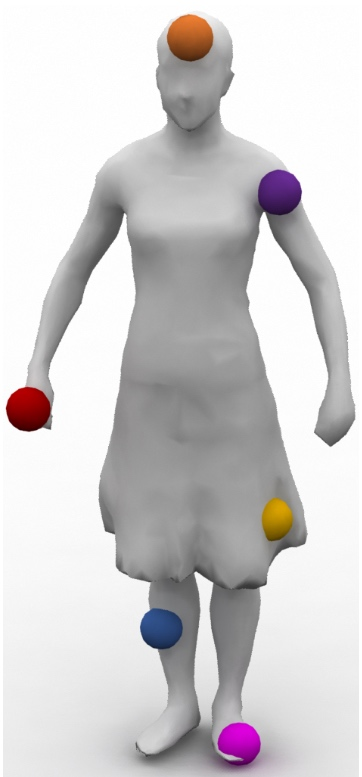
\includegraphics[height=.27\linewidth]{gw/source}
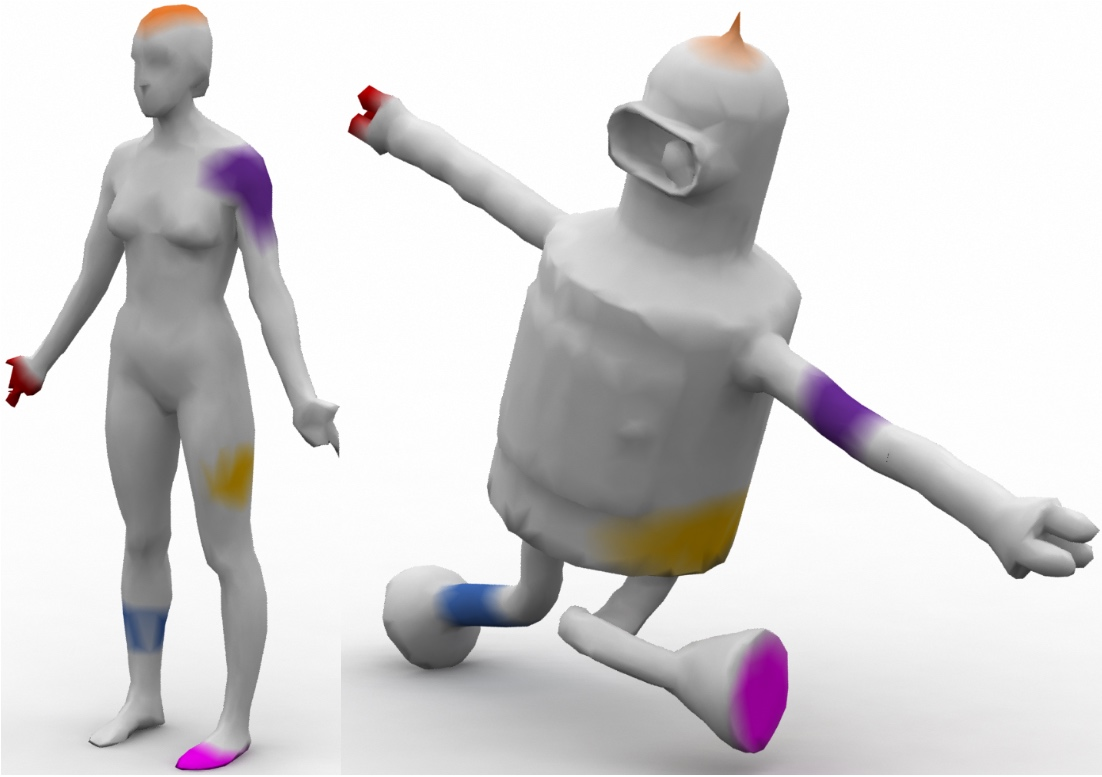
\includegraphics[height=.27\linewidth]{gw/target-surf}
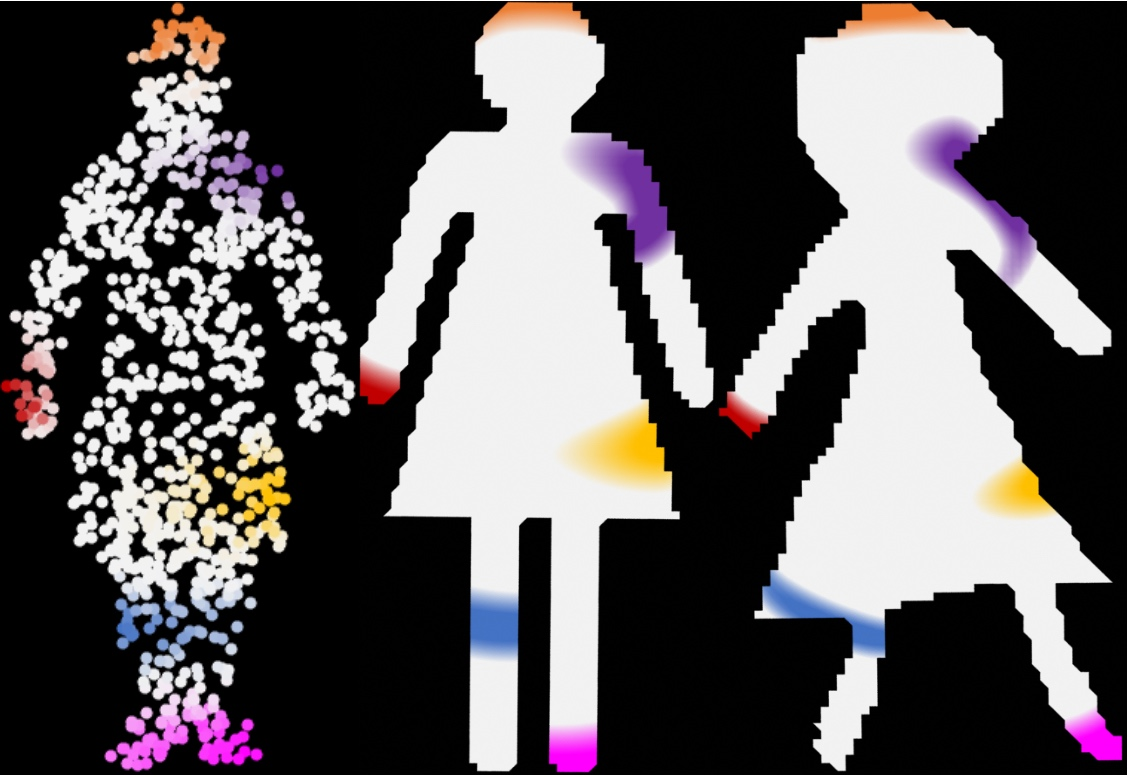
\includegraphics[height=.27\linewidth]{gw/target-2d}
\caption{\label{fig-gw-sinkhorn}
Sinkhorn反復~\eqref{eq-gw-sinkh}を用いてGW問題~\eqref{eq-gw-entropy}を解くことにより計算されたファジー対応の例。~\citep{2016-solomon-gw}より抜粋。
}
\end{figure}





\chapter*{謝辞}
本調査論文の準備の様々な段階で助力してくださった多くの同僚、共同研究者、学生の皆様に感謝申し上げたい。彼らの意見の一部は本研究を形作っており、特に以下の方々に感謝したい：Jean-David Benamou、Yann Brenier、Guillaume Carlier、Vincent Duval、およびInriaのMOKAPLANチーム全体；Francis Bach、Espen Bernton、Mathieu Blondel、Nicolas Courty、R\'emi Flamary、Alexandre Gramfort、Young-Heon Kim、Daniel Matthes、Philippe Rigollet、Filippo Santambrogio、Justin Solomon、Jonathan Weed；そしてこれらのテーマに関する現在および過去の学生からのフィードバック、特にGwendoline de Bie、L\'ena\"ic Chizat、Aude Genevay、Hicham Janati、Th\'eo Lacombe、Boris Muzellec、Fran\c ois-Pierre Paty、Vivien Seguyの各氏。


\bibliographystyle{plainnat}
\bibliography{./biblio/all}

\end{document}
